%%
%%%%*************************Document Class Declaration*******************************
%%
\documentclass{njustThesis}% thesis template of the Nanjing Univ of Sci & Tech
%% Options:
%% [draftinfo] % show draft version information
%%%%% --------------------------------------------------------------------------------
%%
%%%%**************************Command Define and Settings***************************
%%
\usepackage[njust]{sty/commons}% common settings
\usepackage{sty/custom}% user defined commands
\usepackage[textsize=scriptsize]{todonotes}
\usepackage{physics} % 这个包含了常用数学物理方程的符号
\usepackage{nicefrac}
% \usepackage{gensymb}
\usepackage{floatrow}
\usepackage{makecell}
%%%%%%%%%%%%%%%%%%%%%%%%%%%%%%%%%%%%%%%
% 设置代码列表框
\usepackage{listings}

\lstset{
    numbers=left,
    numberstyle=\small,
    numbersep=8pt,
    frame = single,
    framexleftmargin=15pt}
% 表头置于表上
%\usepackage{float}
\floatstyle{plaintop}
\restylefloat{table}
%%%%%%%%%%%%%%%%%%%%%%%%%%%%%%%%%%%%%%%%
\usepackage{tabularx}
\usepackage{tabulary}
%%%%%%%%%%%%%%%%%%%%%%%%%%%%%%%%%%%%%%%%
\newcolumntype{L}[1]{>{\hsize=#1\hsize\raggedright\arraybackslash}X}%
\newcolumntype{R}[1]{>{\hsize=#1\hsize\raggedleft\arraybackslash}X}%
%\newcolumntype{C}[2]{>{\hsize=#1\hsize\columncolor{#2}\centering\arraybackslash}X}%
\newcolumntype{C}[1]{>{\hsize=#1\hsize\centering\arraybackslash}X}%
\newcolumntype{M}[1]{>{\centering\arraybackslash}m{#1}}
%%%%%%%%%%%%%%%%%%%%%%%%%%%%%%%%%%%%%%%%
\newcommand{\todoZN}[1]{\todo[color=red!20]{ZN: #1}}
\newcommand{\todoiZN}[1]{\todo[color=red!20,inline]{ZN: #1}}

\newcommand{\todoWCJ}[1]{\todo[color=blue!20]{WCJ: #1}}
\newcommand{\todoiWCJ}[1]{\todo[color=blue!20,inline]{WCJ: #1}}
%
\sisetup{range-phrase=\textup{--}}


% Custom math
\newcommand{\tbf}{\textbf}% text bold
\newcommand{\tit}{\textit}% text italic
\newcommand{\tsl}{\textsl}% text slanted
\newcommand{\tsc}{\textsc}% text small cap
\newcommand{\ttt}{\texttt}% text typewriter
\newcommand{\trm}{\textrm}% text roman
\newcommand{\tsf}{\textsf}% text sans serif
\newcommand{\tup}{\textup}% text upright
\newcommand{\mbf}{\mathbf}% math bold
\providecommand{\mit}{\mathit}% math italic
\newcommand{\msf}{\mathsf}% math sans serif
\newcommand{\mrm}{\mathrm}% math roman
\newcommand{\mtt}{\mathtt}% math typewriter
\newcommand{\dcdot}{\mathbf{:}}

\DeclareMathAlphabet\mathbfcal{OMS}{cmsy}{b}{n}
\newcommand{\fourtens}{\mathbfcal}
%%%%% ------------------------------------------------------------------------------------------
%%%%*********************************Content**********************************************
\newlength{\jeroenlen}
\newenvironment{shizhong}
{\settowidth{\jeroenlen}{式中:}%
    \begin{description}[font=\normalfont,leftmargin=\jeroenlen,labelwidth=0pt,labelsep=0pt]
        \item[式中:]%
        \begin{itemize}[leftmargin=1.5em,labelsep=.5em, label={}]}
        {\end{itemize}
    \end{description}}
%%
\definecolor{gray}{rgb}{0.4,0.4,0.4}
\definecolor{darkblue}{rgb}{0.0,0.0,0.6}
\definecolor{cyan}{rgb}{0.0,0.6,0.6}

\lstset{
    basicstyle=\ttfamily,
    columns=fullflexible,
    showstringspaces=false,
    commentstyle=\color{gray}\upshape
}

\lstdefinelanguage{XML}
{
    morestring=[b]",
    morestring=[s]{>}{<},
    morecomment=[s]{<?}{?>},
    stringstyle=\color{black},
    identifierstyle=\color{darkblue},
    keywordstyle=\color{cyan},
    morekeywords={xmlns,version,type}% list your attributes here
}
\usepackage{threeparttable}
\begin{document}
%%
%%%%% ------------------------------------------------------------------------------------------
%%
%%%%*********************************Frontmatter******************************************
%%
%% Frontmatter of Title page, Table of contents, Preface chapter.
%%
%% >>> Cover
%%
    %%
%%% >>> Title Page
%%
%%
%%%%********************** Chinese Title Page **************************************** 
%%
\classification{}
\confidential{公开}
\UDC{}
%% 标题格式 \title[short title for headers]{Long title of thesis}
\title[南京工业大学硕士论文模板]{南京工业大学硕士论文模板}
\titleUpp{南京工业大学硕士论文模板}
\titleLow{\phantom{we don't have subtitle}}
\author{张三}
\advisor{李四}
\advisortitle{教授}
\coadvisor{王五}
\coadvisortitle{讲师}
\entcoadvisor{马六}
\entcoadvisortitle{高级工程师}
\degree{工程硕士}
\major{XX工程}
\interest{YYYYYYY}
\school{南京工业大学}
\submitdate{2023年7月}
\incoverdate{2023年7月}
%
\titleBackbone{硕\\士\\论\\文\\模\\板}
\schoolBackbone{南\\京\\工\\业\\大\\学}
%%
%%%%********************** English Title Page **************************************** 
%%
\englishtitle{Nanjing TECH University Master Thesis}
\englishauthor{Zhang san}
\englishadvisor{Li Si}
\englishcoadvisor{Wang Wu}
\englishinstitute{Nanjing TECH University}
\englishdate{December, 2023}
\englishdegree{Dissertation}
%%
%%%%********************** Generate CHN & Eng Title *********************************** 
%%% 
%%
\maketitle
%%
\makeincovertitle
%%
\makeenglishtitle
%% make statement page
\makeatletter
\cleardoublepage
\thispagestyle{empty}
\begin{center}
    \statement{
本学位论文是我在导师的指导下取得的研究成果,尽我所知,在本 学位论文中,除了加以标注和致谢的部分外,不包含其他人已经发表或 公布过的研究成果,也不包含我为获得任何教育机构的学位或学历而使 用过的材料。与我一同工作的同事对本学位论文做出的贡献均已在论文 中作了明确的说明。
}%

\accredit{
南京工业大学有权保存本学位论文的电子和纸质文档,可以借阅或 上网公布本学位论文的部分或全部内容,可以向有关部门或机构送交并 授权其保存、借阅或上网公布本学位论文的部分或全部内容。对于保密 论文,按保密的有关规定和程序处理。
}%

\end{center}
\clearpage
\if@twoside
\thispagestyle{empty}
\cleardoublepage
\fi
\makeatother
%%%%*********************************** END *******************************************

%%
%% >>> start frontmatter page No.
%%
    \frontmatter
%%
%% >>> Abstract
%%
    \begin{abstract}

本文是南京工业大学学位论文模板——njtechThesis的使用说明文档。主要内容为介绍\LaTeX{}文档类njtechThesis的用法,以及如何使用\LaTeX{}快速高效地撰写学位论文。

\LaTeX{}是一种基于\TeX{}的排版系统,主要利用命令行代码的形式对文稿进行格式化处理。相对于常用的可视化工具(如MS Word$^{\circledR}$)而言,其能够让作者更加专注于文章本身内容,而较多地将排版等重复任务交给编译系统,尤其是数学公式、参考文献或图标较多的科技文献。针对中文,\LaTeX{}提供有CTeX套装,并且国内较多院校都提供有\LaTeX{}格式的学位论文模板,中文期刊的排版系统中应用也较为广泛。

对于学位论文而言,\LaTeX{}又是体现在模块化处理、公式、图标、交叉引用等方面。模块化处理即将整个文稿切割成多个简单的子模块,然后利用主文件将文稿的子模块链接成一篇完整的文章(和编程语言中模块化、以及商业软件LsDYNA$^{\circledR}$中使用的include命令相同)。另外,排版系统中的格式定义系统也可以单独的模块化,由类文件(.cls)通过命令定义文中需要的版式等格式函数命令,通过格式文件(.sty)包含一些常用的包(package)。如此,文章中的格式信息和文稿中的内容就形成了相对独立的系统。对普通用户而言,只需要书写文稿内容,而将格式信息交由专业排版方进行(如图书馆、出版社等)。公式和图表的优势体现在,格式自动化对齐(相信使用MS的都有过公式窜行和表格窜页的感触)、交叉引用自动编号。

在模块化的基础上,本文模板将南京工业大学学位论文格式进行标准化处理,方便使用方快速查找需要添加的文稿位置。文件夹架构是标准化的基础,将格式信息、文本内容、插图、文献分别布置在sty、tex、img和bib四个文件夹下,由主模块Thesis.tex进行流程控制。

对于用户而言,使用步骤较为简单(注意:中文的文本编辑应采用UTF-8):

1. 下载模版包(https://github.com/jiec827/njtechThesis),解压;

2. 修改学位论文信息(tex/cover.tex),并将对应的内容添加至tex目录下的其他文件内(正文部分额外添加的章节需要在Thesis.tex文件中使用input命令包含);

3. 采用命令{\color{blue}xelatex Thesis.tex}进行编译;

4. 命令行{\color{blue}makeindex Thesis.nlo -s nomencl.ist -o Thesis.nls}生成图表引用和术语链接;

5. 命令行{\color{blue}bibtex Thesis.aux}更新参考文献引用;

6. {\color{blue}xelatex Thesis.tex}重新编译生成pdf文件。

为了更好的完成学位论文这种长篇幅的文稿排版,对格式文件的了解也是有必要的。首先从主文件Thesis.tex着手,把握真个流程思路与文章的对应关系。然后看格式文件/sty,可以从njtechThesis.cls开始,.cfg和.sty较为简单,只是包含一些需要使用的常量、默认值和扩展包等。

小提醒:学习的宝典当然还是google$^{\circledR}$和baidu$^{\circledR}$哦!

本文初衷是趁双旦闲暇,给以后的学位论文排版做点准备工作。有感于开源的精神,特把排版代码放到GitHub$^{\circledR}$上,在开发过程中虽然是以参考和借鉴为主,但仍按照Repository的软件工程开源流程进行操作。希望能够有人多多参与,通过这个简单的开源项目,了解、学习和推广。当然,回到根本,希望这个基于\LaTeX{}的排版项目能够给更多的同学提供一点小帮助。

\keywords{南京工业大学,学位论文,\LaTeX{},模板}
\end{abstract}


\begin{englishabstract}

1 In the beginning was the Word, and the Word was with God, and the Word was God. 2 He was with God in the beginning. 3 Through him all things were made; without him nothing was made that has been made. 4 In him was life, and that life was the light of all mankind. 5 The light shines in the darkness, and the darkness has not overcome it.

6 There was a man sent from God whose name was John. 7 He came as a witness to testify concerning that light, so that through him all might believe. 8 He himself was not the light; he came only as a witness to the light.

9 The true light that gives light to everyone was coming into the world. 10 He was in the world, and though the world was made through him, the world did not recognize him. 11 He came to that which was his own, but his own did not receive him. 12 Yet to all who did receive him, to those who believed in his name, he gave the right to become children of God. 13 children born not of natural descent, nor of human decision or a husband’s will, but born of God.

14 The Word became flesh and made his dwelling among us. We have seen his glory, the glory of the one and only Son, who came from the Father, full of grace and truth.

15 (John testified concerning him. He cried out, saying, “This is the one I spoke about when I said, ‘He who comes after me has surpassed me because he was before me.’”) 16 Out of his fullness we have all received grace in place of grace already given. 17 For the law was given through Moses; grace and truth came through Jesus Christ. 18 No one has ever seen God, but the one and only Son, who is himself God and[b] is in closest relationship with the Father, has made him known.

19 Now this was John’s testimony when the Jewish leaders[c] in Jerusalem sent priests and Levites to ask him who he was. 20 He did not fail to confess, but confessed freely, “I am not the Messiah.”

21 They asked him, “Then who are you? Are you Elijah?”

He said, “I am not.”

“Are you the Prophet?”

He answered, “No.”

22 Finally they said, “Who are you? Give us an answer to take back to those who sent us. What do you say about yourself?”

23 John replied in the words of Isaiah the prophet, “I am the voice of one calling in the wilderness, ‘Make straight the way for the Lord.’”

24 Now the Pharisees who had been sent 25 questioned him, “Why then do you baptize if you are not the Messiah, nor Elijah, nor the Prophet?”

26 “I baptize with[e] water,” John replied, “but among you stands one you do not know. 27 He is the one who comes after me, the straps of whose sandals I am not worthy to untie.”

28 This all happened at Bethany on the other side of the Jordan, where John was baptizing.

29 The next day John saw Jesus coming toward him and said, “Look, the Lamb of God, who takes away the sin of the world! 30 This is the one I meant when I said, ‘A man who comes after me has surpassed me because he was before me.’ 31 I myself did not know him, but the reason I came baptizing with water was that he might be revealed to Israel.”

32 Then John gave this testimony: “I saw the Spirit come down from heaven as a dove and remain on him. 33 And I myself did not know him, but the one who sent me to baptize with water told me, ‘The man on whom you see the Spirit come down and remain is the one who will baptize with the Holy Spirit.’ 34 I have seen and I testify that this is God’s Chosen One.”

(cited from: {\color{blue}{{\it{John: The Word Became Flesh}}}})

\englishkeywords{Nanjing University of Sciences \& Technology (NUST), Thesis, \LaTeX{}
Template}
\end{englishabstract}
%%
%%% >>> List of Content
%%
%\clearpage
    \tableofcontents% contents catalog
    %\addcontentsline{toc}{chapter}{目录}
%% list figures and tables sperately
    \listoffigures%   figures catalog
%\addcontentsline{toc}{chapter}{插图目录}
    \listoftables%    tables catalog
    %\addcontentsline{toc}{chapter}{表格目录}
%% list figures and tables together
    %\listoffiguresandtables
    %\addcontentsline{toc}{chapter}{图表目录}
%%
    % {\centering\printnomenclature}% nomenclature catalog
    % \addcontentsline{toc}{chapter}{术语表}
%%
%%%%% ------------------------------------------------------------------------------------------
%%
%%%%*********************************Mainmatter******************************************
%%
%% Main topics.
    \mainmatter
%%
%%% >>> Main Contents
%%
    
\chapter{引言}
\label{chap:introduction}

考虑到大多数用户可能并无\LaTeX{}使用经验,本模板将\LaTeX{}的复杂性尽可能地进行了封装,开放出简单的接口,以便于使用者可以轻易地使用,同时,对使用\LaTeX{}撰写论文所遇到的一些主要难题,如插入图片、文献索引等,进行了详细的说明,并提供了相应的代码样本,理解了上述问题后,对于初学者而言,使用此模板撰写其学文论文将不存在实质性的困难,所以,如果您是初学者,请不要直接放弃,因为同样作为初学者的我,十分明白让\LaTeX{}变得简单易用的重要性,而这正是本模板所体现的。

该南京工业大学学位论文模板\texttt{njtechThesis}基于中科院大学学位论文\texttt{njtechThesis}模板(https://github.com/mohuangrui/njtechThesis)发展而来,\texttt{njtechThesis}文档类的基础架构为ctexbook文档类。当前\texttt{njtechThesis}模板基本满足最新的南京工业大学学位论文撰写要求和封面设定(http://gs.njtech.edu.cn/a/xwgl/xwsq/20130508/82.html)。模板提供了pdflatex 或xelatex (默认,推荐) 编译方式,完美地支持中文书签、中文渲染、中文粗体显示、拷贝pdf中的文本到其他文本编辑器等特性,此外,对模板的文档结构进行了精心设计,撰写了编译脚本提高模板的易用性和使用效率。

宏包的目的是简化学位论文的撰写,模板文档的默认设定是十分规范的,从而论文作者可以将精力集中到论文的内容上,而不需要在版面设置上花费精力。 同时,在编写模板的\LaTeX{}文档代码过程中,作者对各结构和命令进行了十分详细的注解,并提供了整洁一致的代码结构,对文档的仔细阅读可以为初学的您提供一个学习\LaTeX{}的窗口。除此之外,整个模板的架构十分注重通用性,事实上,本模板不仅是南京工业大学学位论文模板,同时,也是使用\LaTeX{}撰写中英文article或book的通用模板,并为使用者的个性化设定提供了接口和相应的代码。

\section{系统要求}
\label{sec:sysRequire}

\texttt{njtechThesis}宏包可以在目前大多数的\TeX{}系统中使用,例如C\TeX{}、MiK\TeX{}、te\TeX{}。考虑到大多数用户将是Windows使用者,推荐安装最新的C\TeX{}套装(2.9.1及其以上版本),C\TeX{}套装中包含了本模板中出的各类宏包,用户无需额外的设置即可使用。

\texttt{njtechThesis}宏包通过\texttt{ctexbook}宏包来获得中文支持。\texttt{ctexbook}宏包提供了一个统一的中文\LaTeX{}书籍文档框架,底层支持CCT和CJK两种中文\LaTeX{}系统。

此外,\texttt{njtechThesis}宏包还使用了宏包mathtools、amsthm、amsfonts、amssymb、bm、natbib和hyperref。目前大多数的\TeX{}系统中都包含有这些宏包。

目前已经测试的系统和版本为:
%% ++++++++++++++++++++++++++++++++++++++
\begin{enumerate}
\item texlive-2023(MacTeX on Mac OSX);

\item texlive-2023(Windows OS)。

\end{enumerate}
%% ++++++++++++++++++++++++++++++++++++++

{\color{blue}{说明:1. texlive一般每年更新一次,尽量使用最新版本,以免有些新的功能不能使用;

2. 在近期的论文版本中参考文献开始使用biber进行编译。

}}

\section{下载与使用}
\label{sec:howtouse}
njtechThesis 模版包的最新版本可以从 https://github.com/zhangning737, 网站下载。既可以直接通过网站右侧命令下载包,也可以通过命令行下载(推荐,但是需要安装git)

\begin{center}
  {\color{blue}{git clone https://github.com/zhangning737/njtechThesisMaster.git}}
\end{center}


njtechThesis 宏包包含4个文件夹和主函数Thesis.tex,另外附有说明文档和示例模版。文件架构如下:

0. LICENSE: GPL证书,开源性质

1. README.md: 项目介绍信息,包含使用和其他基本信息

2. HowToUseIt.pdf: 该项目生成的一个样本PDF文件(最近一次推送版本)

3. njtechThesis.tex: 主函数

4. sty: (directory) 排版格式信息文件夹

5. tex: (directory) 论文内容文件夹,包含封面、摘要、章节、附录等

6. img: (directory) 论文中使用到的插图文件夹,包含学校logo和章节图片

7. bib: (directory) 参考文献文件夹,使用bibTeX格式

使用基本流程见READ.md文件或中文摘要中的描述。基本思路是,分别将封面、章节和附件中的内容更新到对应的*.tex文件,然后第一次编译刷新tex系统,在更新对应的引用文件系统,最后一次编译获得最终排版稿件。

值得提醒的是,宏包中提供的范例文档《HowToUseIt.pdf》,对使用过程经常需要使用到的命令行进行的例句,尤其是插入图片时会遇到的单列、多列问题,表格的三线、多线,交叉引用等问题,都通过具体实例给出。对于具体用户而言,可以直接采用替换文中引用文件名的方式快速入门使用。

由于笔者个人的时间精力有限,可能会有一些尚未想到的很多方面,往广大师生朋友多多交流互动!

\section{问题反馈}
\label{sec:FandQ}

\subsection{目前尚存在的问题}
\label{sec:remainingProblem}
截止此次编译版本,\texttt{njtechThesis}尚未满足的设计项(设计标准参见第~\ref{app:format}章)包含:

1. 术语表的页眉尚未设置完整,因此未在编译中添加术语表;

2. 一级标题(chapter)的行距问题存在疑问,段前行距略显大;

% 3. 中文参考文献在列表时,作者(4个以上)后面的“et al”需要在*.bbl文件中手动替换为“等”。


%
    \chapter{泥岩流变力学特性试验研究}
\label{chap:theory}
流变特性作为岩石最重要的力学性质之一,与岩土工程的长期稳定性和安全性密切相关。
为了深入分析山体与其内部隧道相互作用下的变形时效特性,必须对岩石进行流变
力学试验,得出岩石流变行为及破坏规律,为岩石流变本构模型的建立奠定基础。在进行流变试验之前,需要对其进行常规三轴压缩试验,根据压缩试验得到的该种岩石基本的抗压强度和变形特性,设计进行相应的三轴流变试验,得出岩石流变行为及破坏规律,为岩石流变本构模型的建立奠定基础。
本节主要介绍三轴流变试验的过程及数据分析。
为了开展。。。。。。。研究,获取参数,针对xxxx的岩石,开展了xxx的实验。本章对实验的过程和结果进行了阐述。

%\section{工程地质概况}

%流变特性作为岩石最重要的力学性质之一,与岩土工程的长期稳定性和安全性密切相关。
%为了深入分析山体与其内部隧道相互作用下的变形时效特性,必须对岩石进行流变
%力学试验,得出岩石流变行为及破坏规律,为岩石流变本构模型的建立奠定基础。在进行流变试验之前,需要对其进行常规三轴压缩试验,根据压缩试验得到的该种岩石基本的抗压强度和变形特性,设计进行相应的三轴流变试验,得出岩石流变行为及破坏规律,为岩石流变本构模型的建立奠定基础。
%

\section{试样及试验仪器简介}
本文以xxx为研究背景,选取xxx的泥岩为研究对象,试验所需试样均为现场直接钻芯所得。将岩样制作成直径\SI{50}{mm}、高度\SI{100}{mm}标准试样,试
件满足两端面不平行度误差不大于\SI{0.05}{mm}、沿高度方向直径误差不大于\SI{0.03}{mm}以及端面与试件轴线的最大偏差不大于\SI{0.25}{\degree}等要求,现场钻取的岩芯以及制作好的试样分如图~\ref{fig:2-1}所示。

\begin{figure}[ht!]
    \centering
    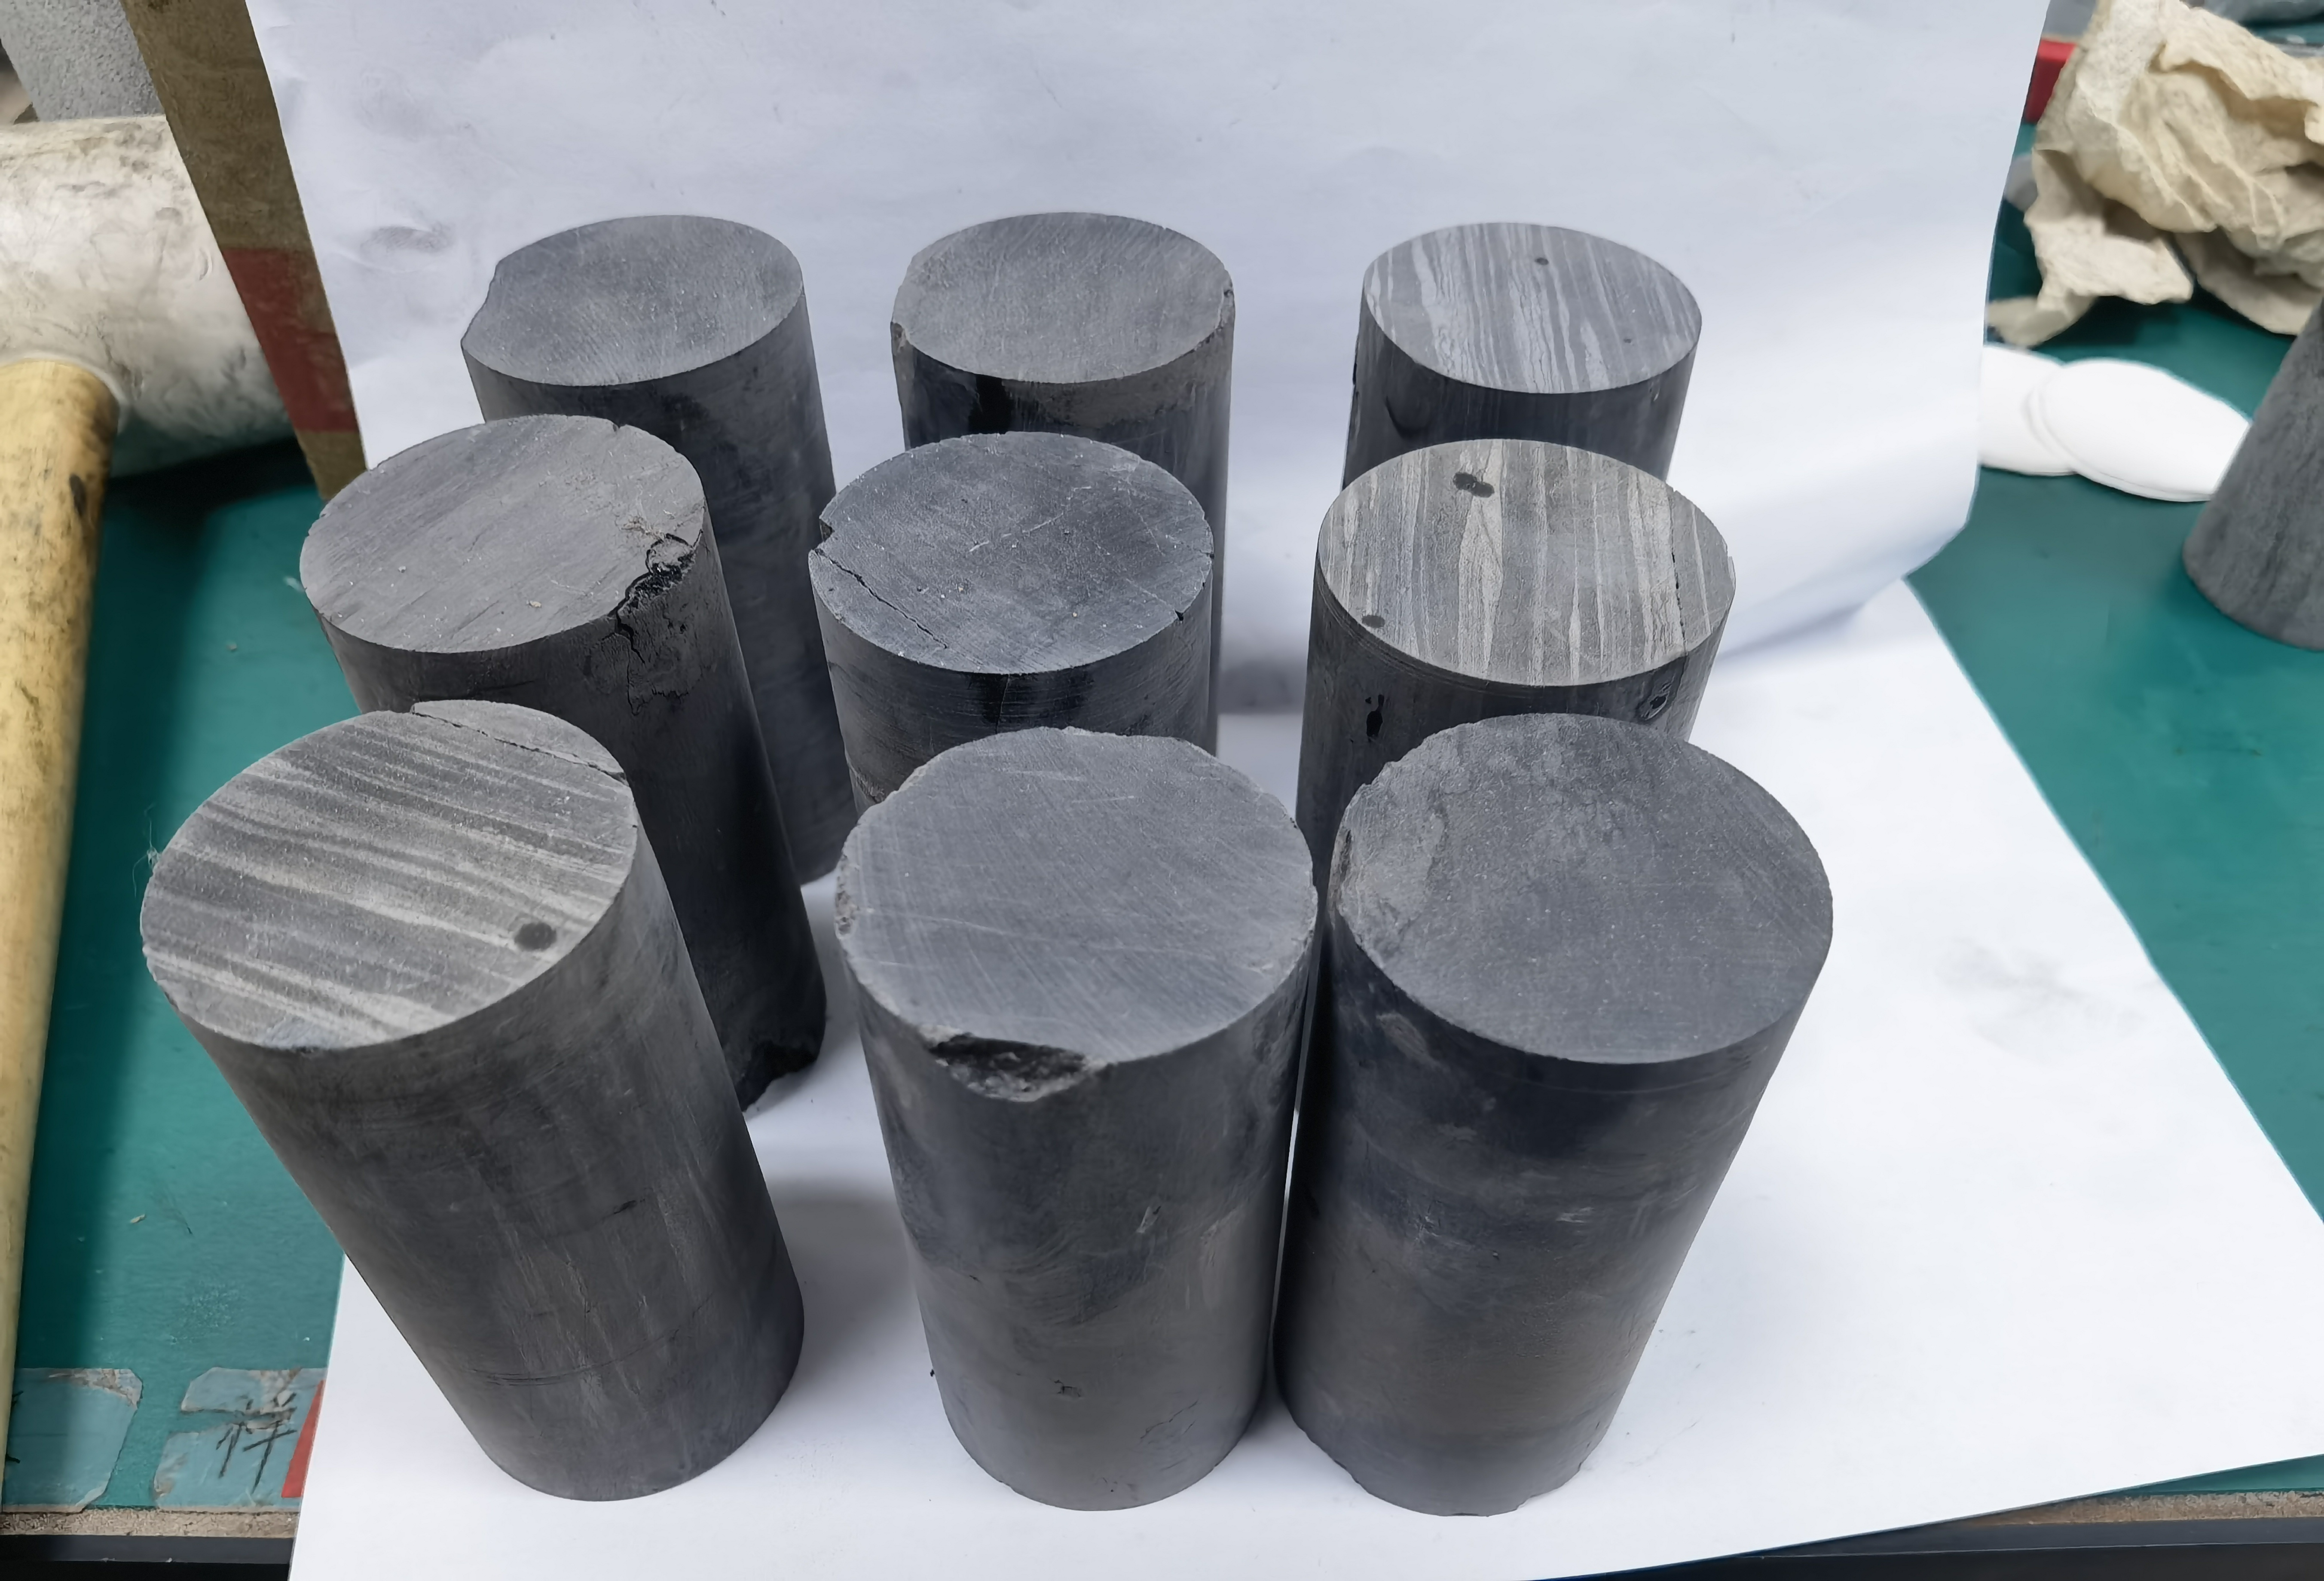
\includegraphics[width=0.5\textwidth]{img/chap2/试样制备.jpg}
    \caption{泥岩试样}
    \label{fig:2-1}
\end{figure}

本次试验在多尺度多场耦合岩石力学试验室完成,使用的设备为法国TOP Industrie公司生产三轴流变仪(如图2.2所示)和气体渗透控制面板。

三轴流变仪于2016年12月完成安装测试,设计最大压力室工作围压为\SI{150}{MPa},最大工作孔压为\SI{150}{MPa},轴向压力最大可达200吨。该设备主要由三轴压力室、轴压伺服泵、围压伺服泵、水压伺服泵、气渗系统、加热装置、超声波测试系统和计算机控制系统组成,可实现岩石常规三轴压缩试验、流变试验、渗透试验以及温度-流体-力学-化学等多场耦合试验,适用范围广,测量精度高。压力控制采用高精度电控伺服高压泵,测量精度可达\SI{0.01}{MPa};轴向位移测量使用两只高灵敏度的位移传感器,可直接输出被测试样的轴向位移值,量程20mm,测量精度达\SI{e-3}{mm};径向位移测量使用应变片式侧向应变仪,输出全桥电路压敏电阻的电压变化值,换算求得径向应变,测量精度达\SI{e-3}{mv/v}。该系统可实现多种方式加载压力,其中轴向压力可选择轴向位移控制、压力控制、流量控制、环向位移控制等加载方式。

\begin{figure}[ht!]
    \centering
    \subfigure[系统图]
    {
        \begin{minipage}{8.6cm}
            \centering
            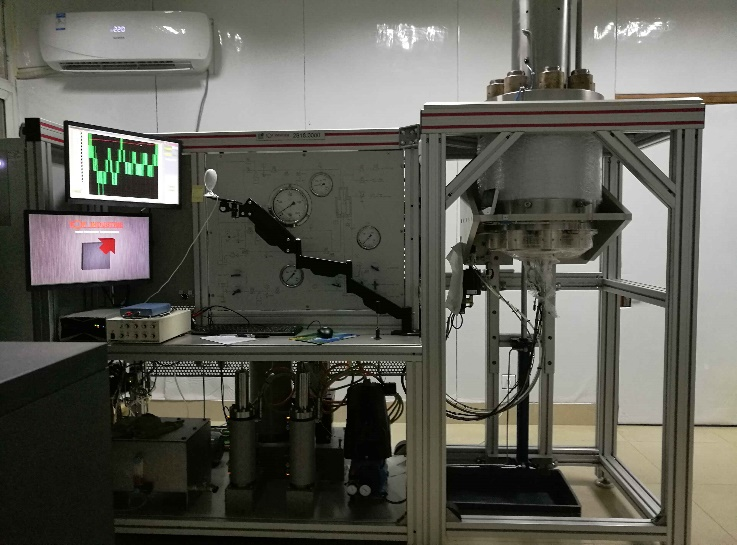
\includegraphics[width=0.9\textwidth]{img/chap2/Multi-scale and multi-field coupling triaxial tester-1.png}
        \end{minipage}
    }
    \subfigure[围岩室]
    {
        \begin{minipage}{5.3cm}
            \centering
            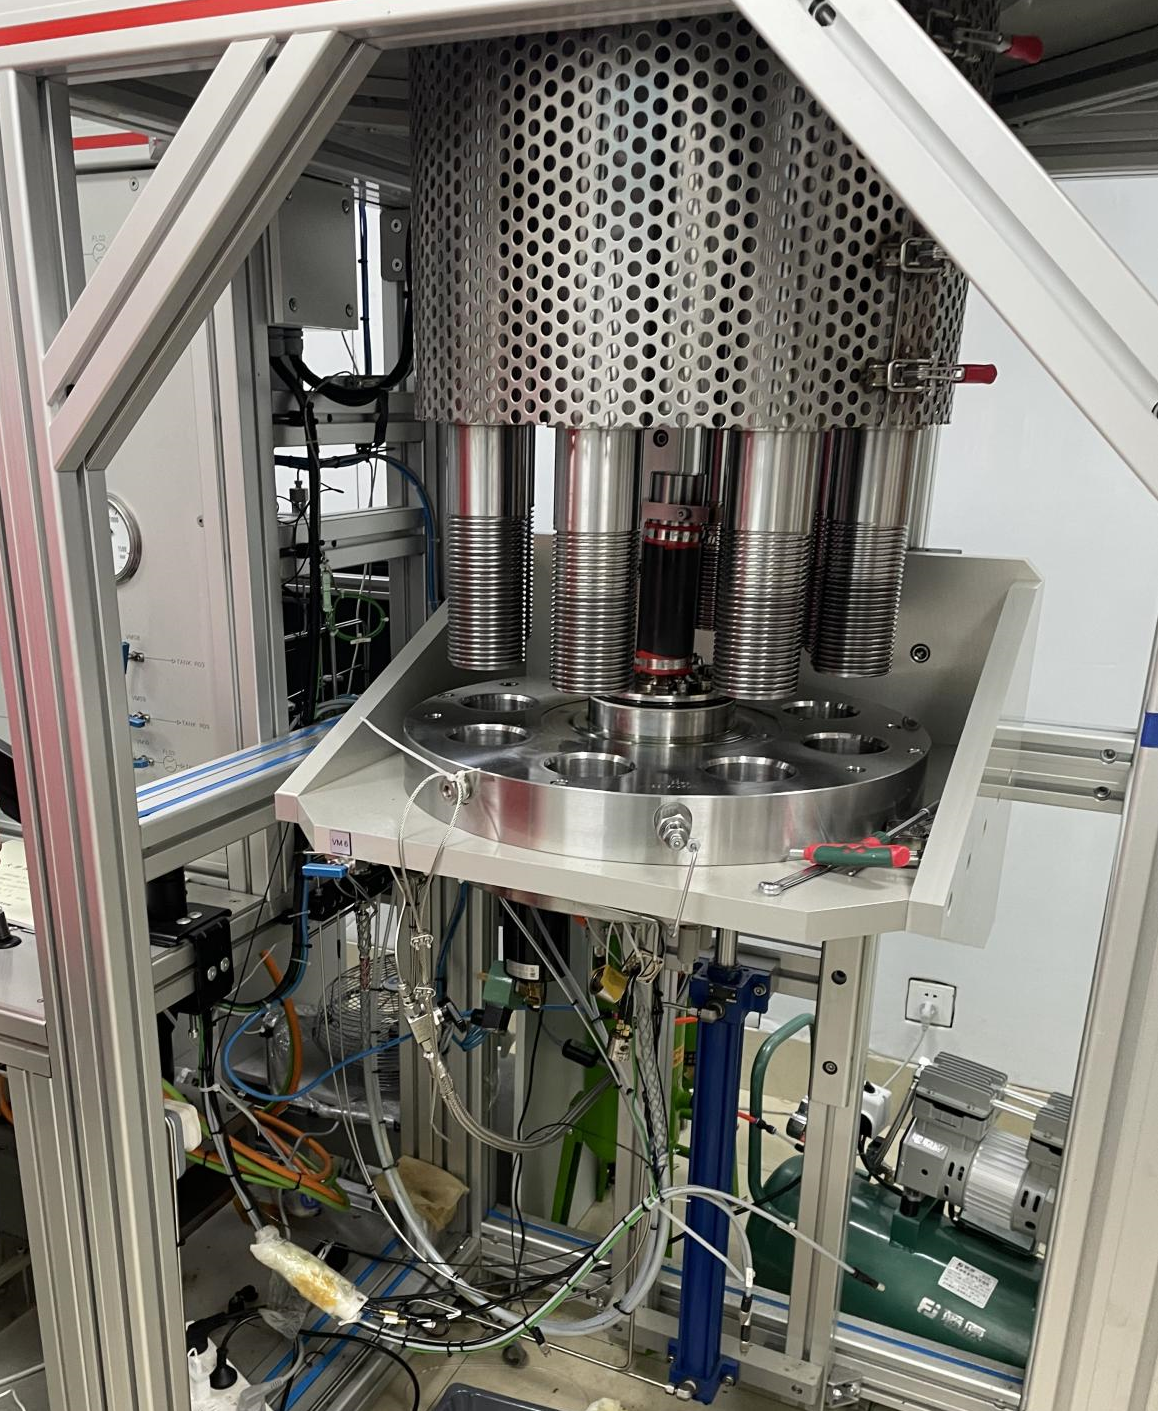
\includegraphics[width=0.9\textwidth]{img/chap2/Multi-scale and multi-field coupling triaxial tester-2.png}
        \end{minipage}
    }
    \caption{多尺度多场耦合三轴试验仪}
    \label{fig:2-2}
\end{figure}

\section{实验方案}

%为什么开展,单轴,三轴,及单三轴流变,方案列表。

\section{泥岩单/三轴压缩实验}
\subsection{试验过程}\label{section:试验过程}
试样三轴压缩试验方案和步骤如下:

(1)试样选取及测量:首先剔除外观有明显缺口、裂缝和节理的试样,选取均质性较好的试样,确定初步筛选后的试样的基本几何和物理参数,包括试样的长度、直径、质量等,通过计算得到密度。试样尺寸的测量采用\SI{0.01}{mm}精度的游标卡尺,在三个不同的位置测量然后取平均值;试样质量的测量使用\SI{0.01}{g}精度的天平,称重三次取平均值,完成后对试样进行编号(如图~\ref{fig:2-3});

(2)试样安装:将试样套入内径\SI{50}{mm}的橡皮套中后将其放置在底座上,试样两端需各放置一片滤纸用于防止试样破坏后的岩石碎屑进入底座的气体通道。之后将压头套入橡皮套放置于试样顶部,橡皮套两端用小宽度喉箍固定密封,防止围压室的液压油进入橡皮套;

(3)充油加围压:本次三轴试验的围压为\SI{5}{MPa}、\SI{10}{MPa}、\SI{15}{MPa}三个等级。首先密封压力室,用低压泵向压力室内充油,再用围压泵将围压加至试验设定的围压值,并维持恒定,围压加载速率为\SI{3}{MPa/min},加载到预定的围压等级后停止加载;

(4)接触加偏应力:围压加载完成后可进行施加偏应力,需要指出的是在施加偏应力前,必须将试样与三轴伺服仪轴压压头进行接触,可手动操作向轴压压力室加油,待轴向应变变化说明已经接触,且接触后要卸载此时的偏应力值到零,最后加满轴压泵,采用速度加载方式,设置大于岩石预估最大偏应力的轴向应力上限值,加载速率设置为\SI{0.02}{mm/min},加载至试样破坏;

(5)待试验全部完成后将气体面板和进气口阀门关闭,将偏压卸载至\SI{0}{MPa},再将围压卸至\SI{0}{MPa},排油结束后即可拆样进行下一步实验。

对于单轴压缩实验而言,试验方案与步骤与上述三轴压缩试验步骤基本一致,只是在试样安装完毕后,不需要通过油泵对试样充油施加围压,直接施加轴向应力即可。

后续试验需要确定泥岩试样的基本变形特性和抗压强度值,在明确了以上目的后,
我们对试样设计、进行了单轴和三轴压缩试验。考虑到一组试验测得的数据可能存在偶然性和较大的误差,因此单轴压缩试验共计进行了三组,我们对三组试验获得的抗压强度求平均值,以此平均值作为后续单轴流变试验的基础强度值。而三轴压缩试验因为时间和试样数量所限,只在每种围压下完成一个试样的试验,具体试验方案如下表~\ref{tab:泥岩三轴压缩试验工况表}

\begin{figure}[ht!]
    \centering
    \subfigure[试样编号]
    {
        \begin{minipage}{7cm}
            \centering
            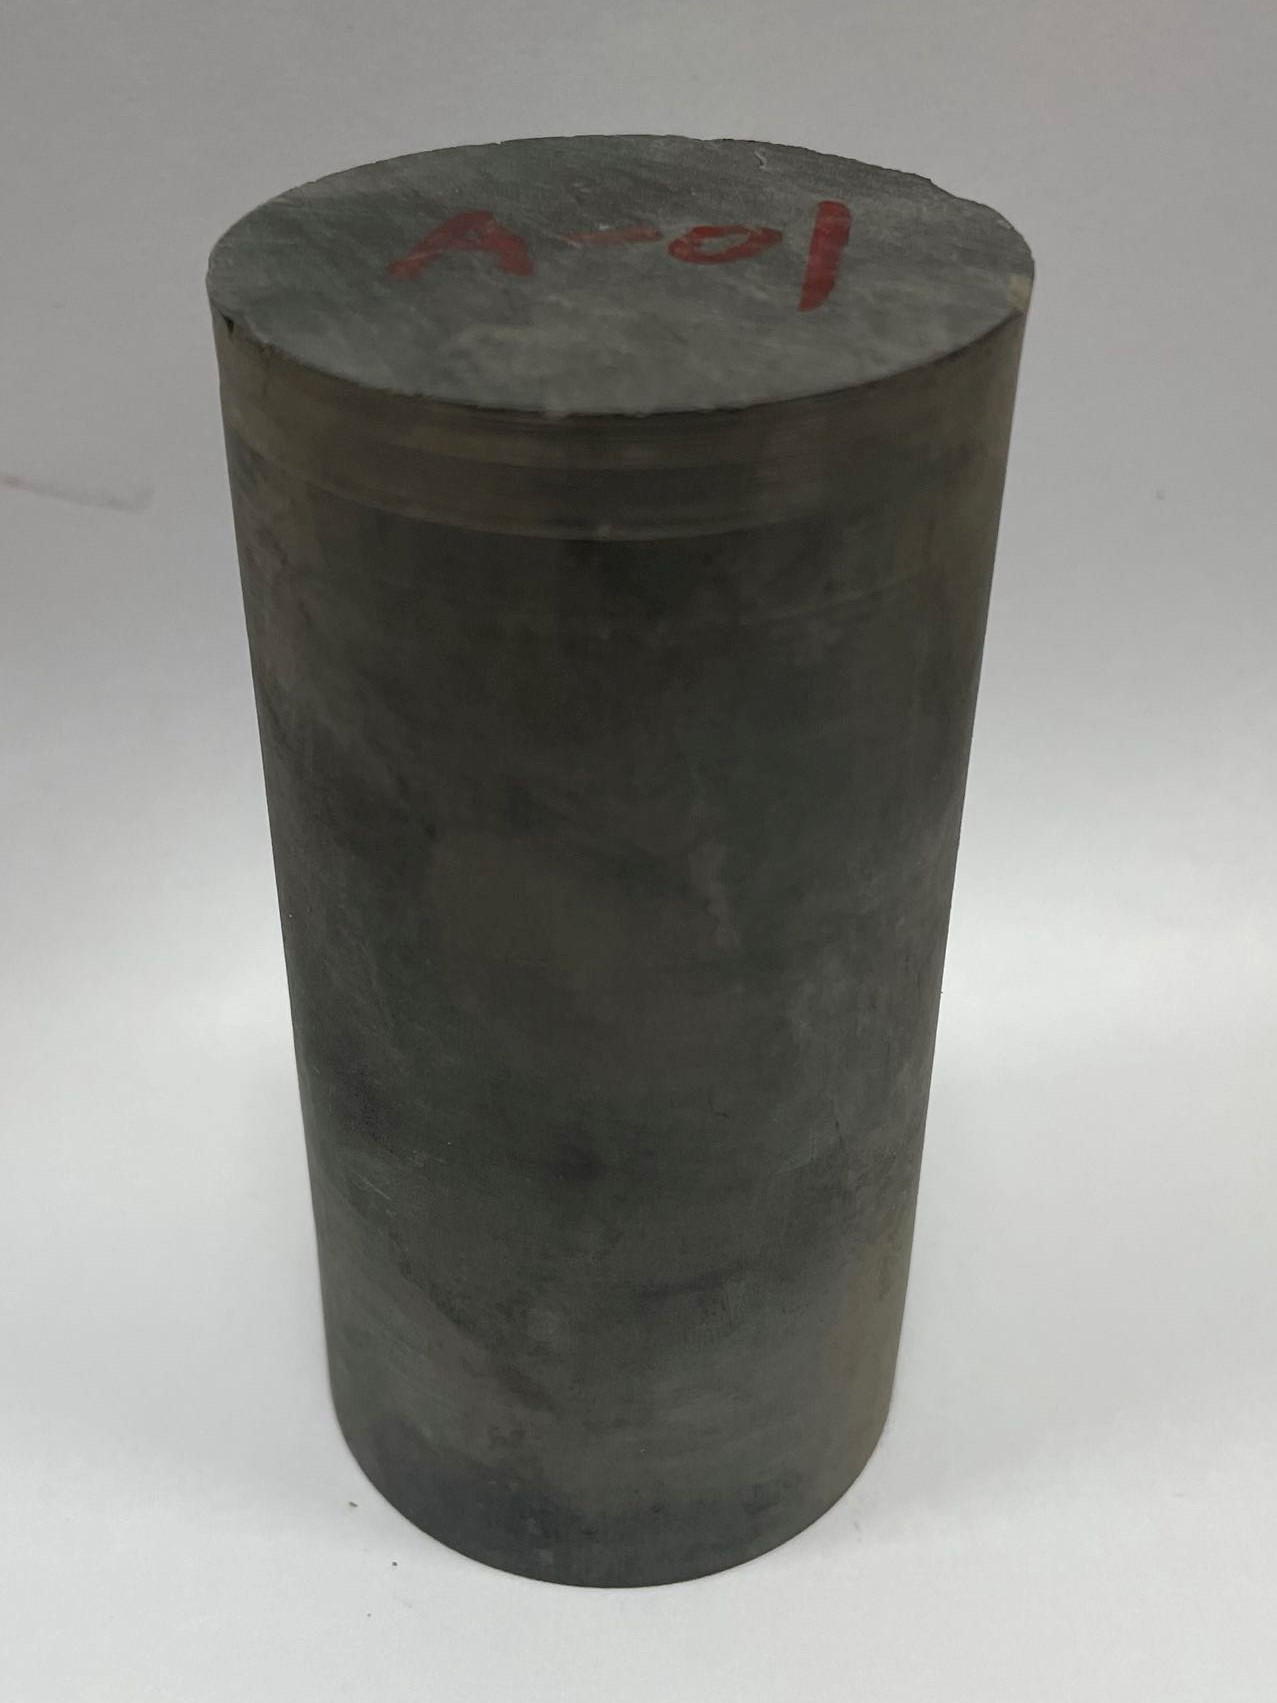
\includegraphics[width=0.9\textwidth]{img/chap2/试样编号.png}
        \end{minipage}
    }
    \subfigure[试样放置]
    {
        \begin{minipage}{7cm}
            \centering
            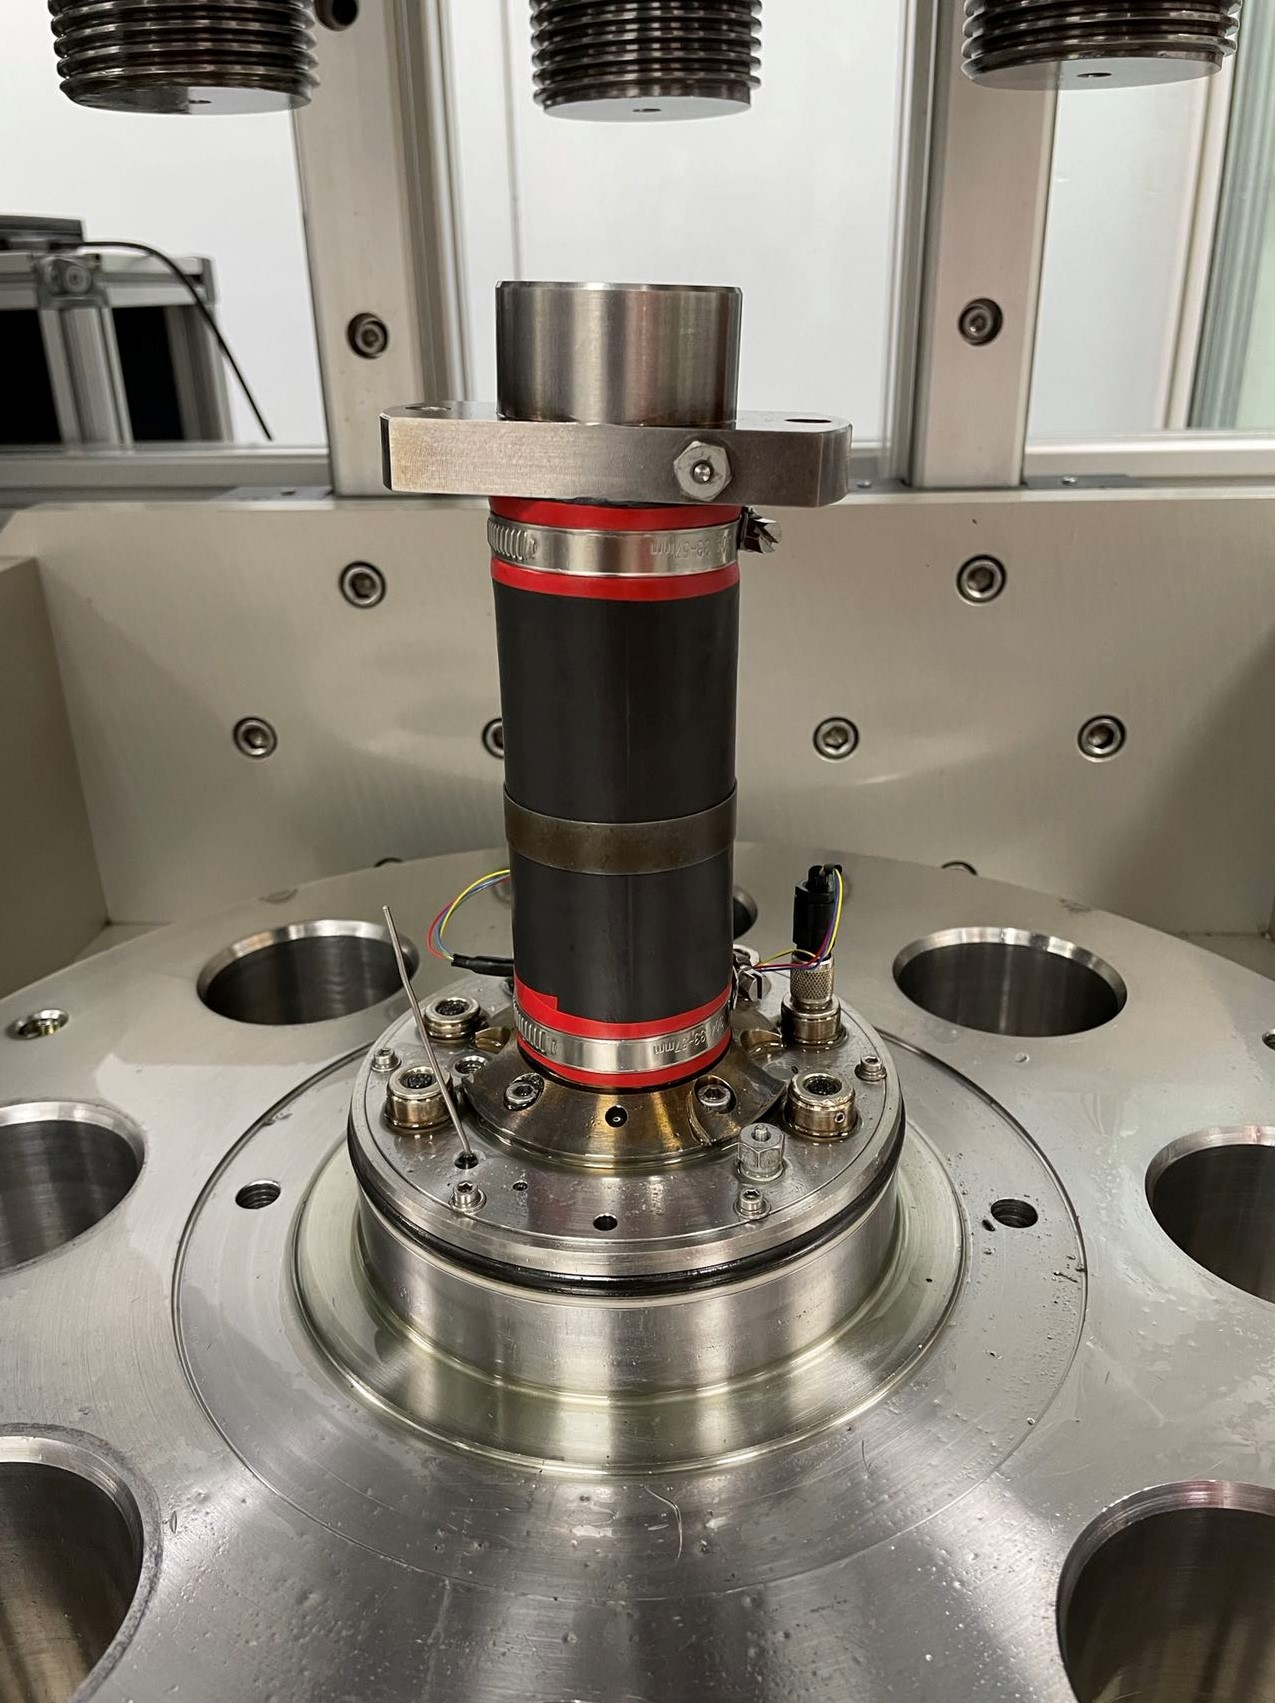
\includegraphics[width=0.9\textwidth]{img/chap2/试样放置.png}
        \end{minipage}
    }
    \caption{试验步骤}
    \label{fig:2-3}
\end{figure}


在本次试验计划中,进行泥岩的单轴压缩及三轴压缩试验,一是为了通过压缩试验获得泥岩的应力-应变曲线,并据此分析泥岩试样的基本力学参数、强度特征及变形特征;二是为了获得试样的抗压强度值,为后续的流变试验做好准备。



\begin{table}[ht!]\small
    \centering
    \begin{tabular}{p{3cm}<{\centering} p{3cm}<{\centering} p{3cm}<{\centering} p{3cm}<{\centering}}
        \toprule
        试样编号  & 围压(MPa)  &  试样高度h(mm)   &  试样直径d(mm)\\
        \midrule
        A-01        & 0  &   98.47  &  50.10   \\ 
        A-02        & 0  &   99.17  &  49.29   \\ 
        A-03        & 0  &   99.82  &  50.16  \\ 
        \midrule
        B-01        & 5  &   99.86  &  49.30    \\ 
        B-02        & 10 &   100.31 &  49.83    \\ 
        B-03        & 15 &   99.78  &  49.74 \\ 
        \bottomrule
    \end{tabular}
    \caption{泥岩三轴压缩试验工况表}
    \label{tab:泥岩三轴压缩试验工况表}
\end{table}



\subsection{试样破坏特征分析}
泥岩试样在不同的围压水平下表现出不同的破坏形态,下图展示了进行三轴压缩试验的试样破坏后的形态:
\begin{figure}[ht!]
    \centering
    \subfigure[A-01]
    {
        \begin{minipage}{7cm}
            \centering
            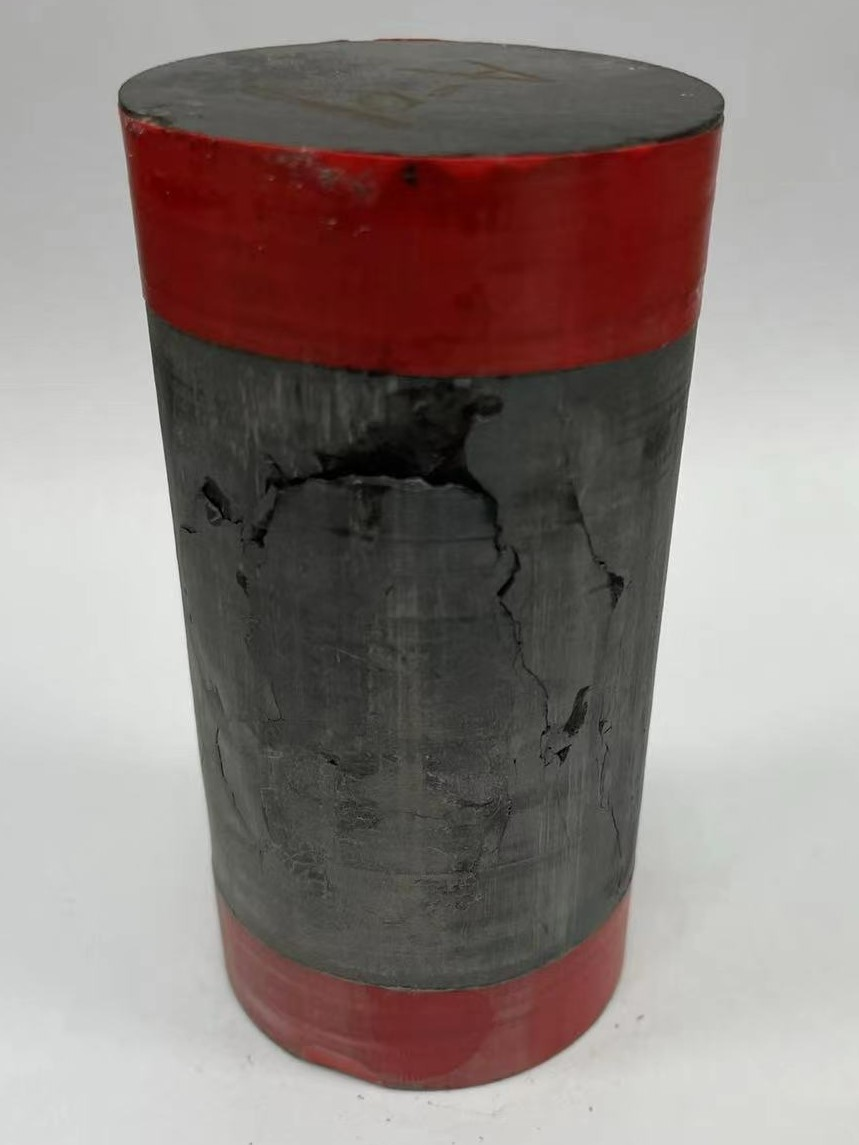
\includegraphics[width=0.9\textwidth]{img/chap2/A-01.jpg}
        \end{minipage}
    }
    \subfigure[B-02]
    {
        \begin{minipage}{7cm}
            \centering
            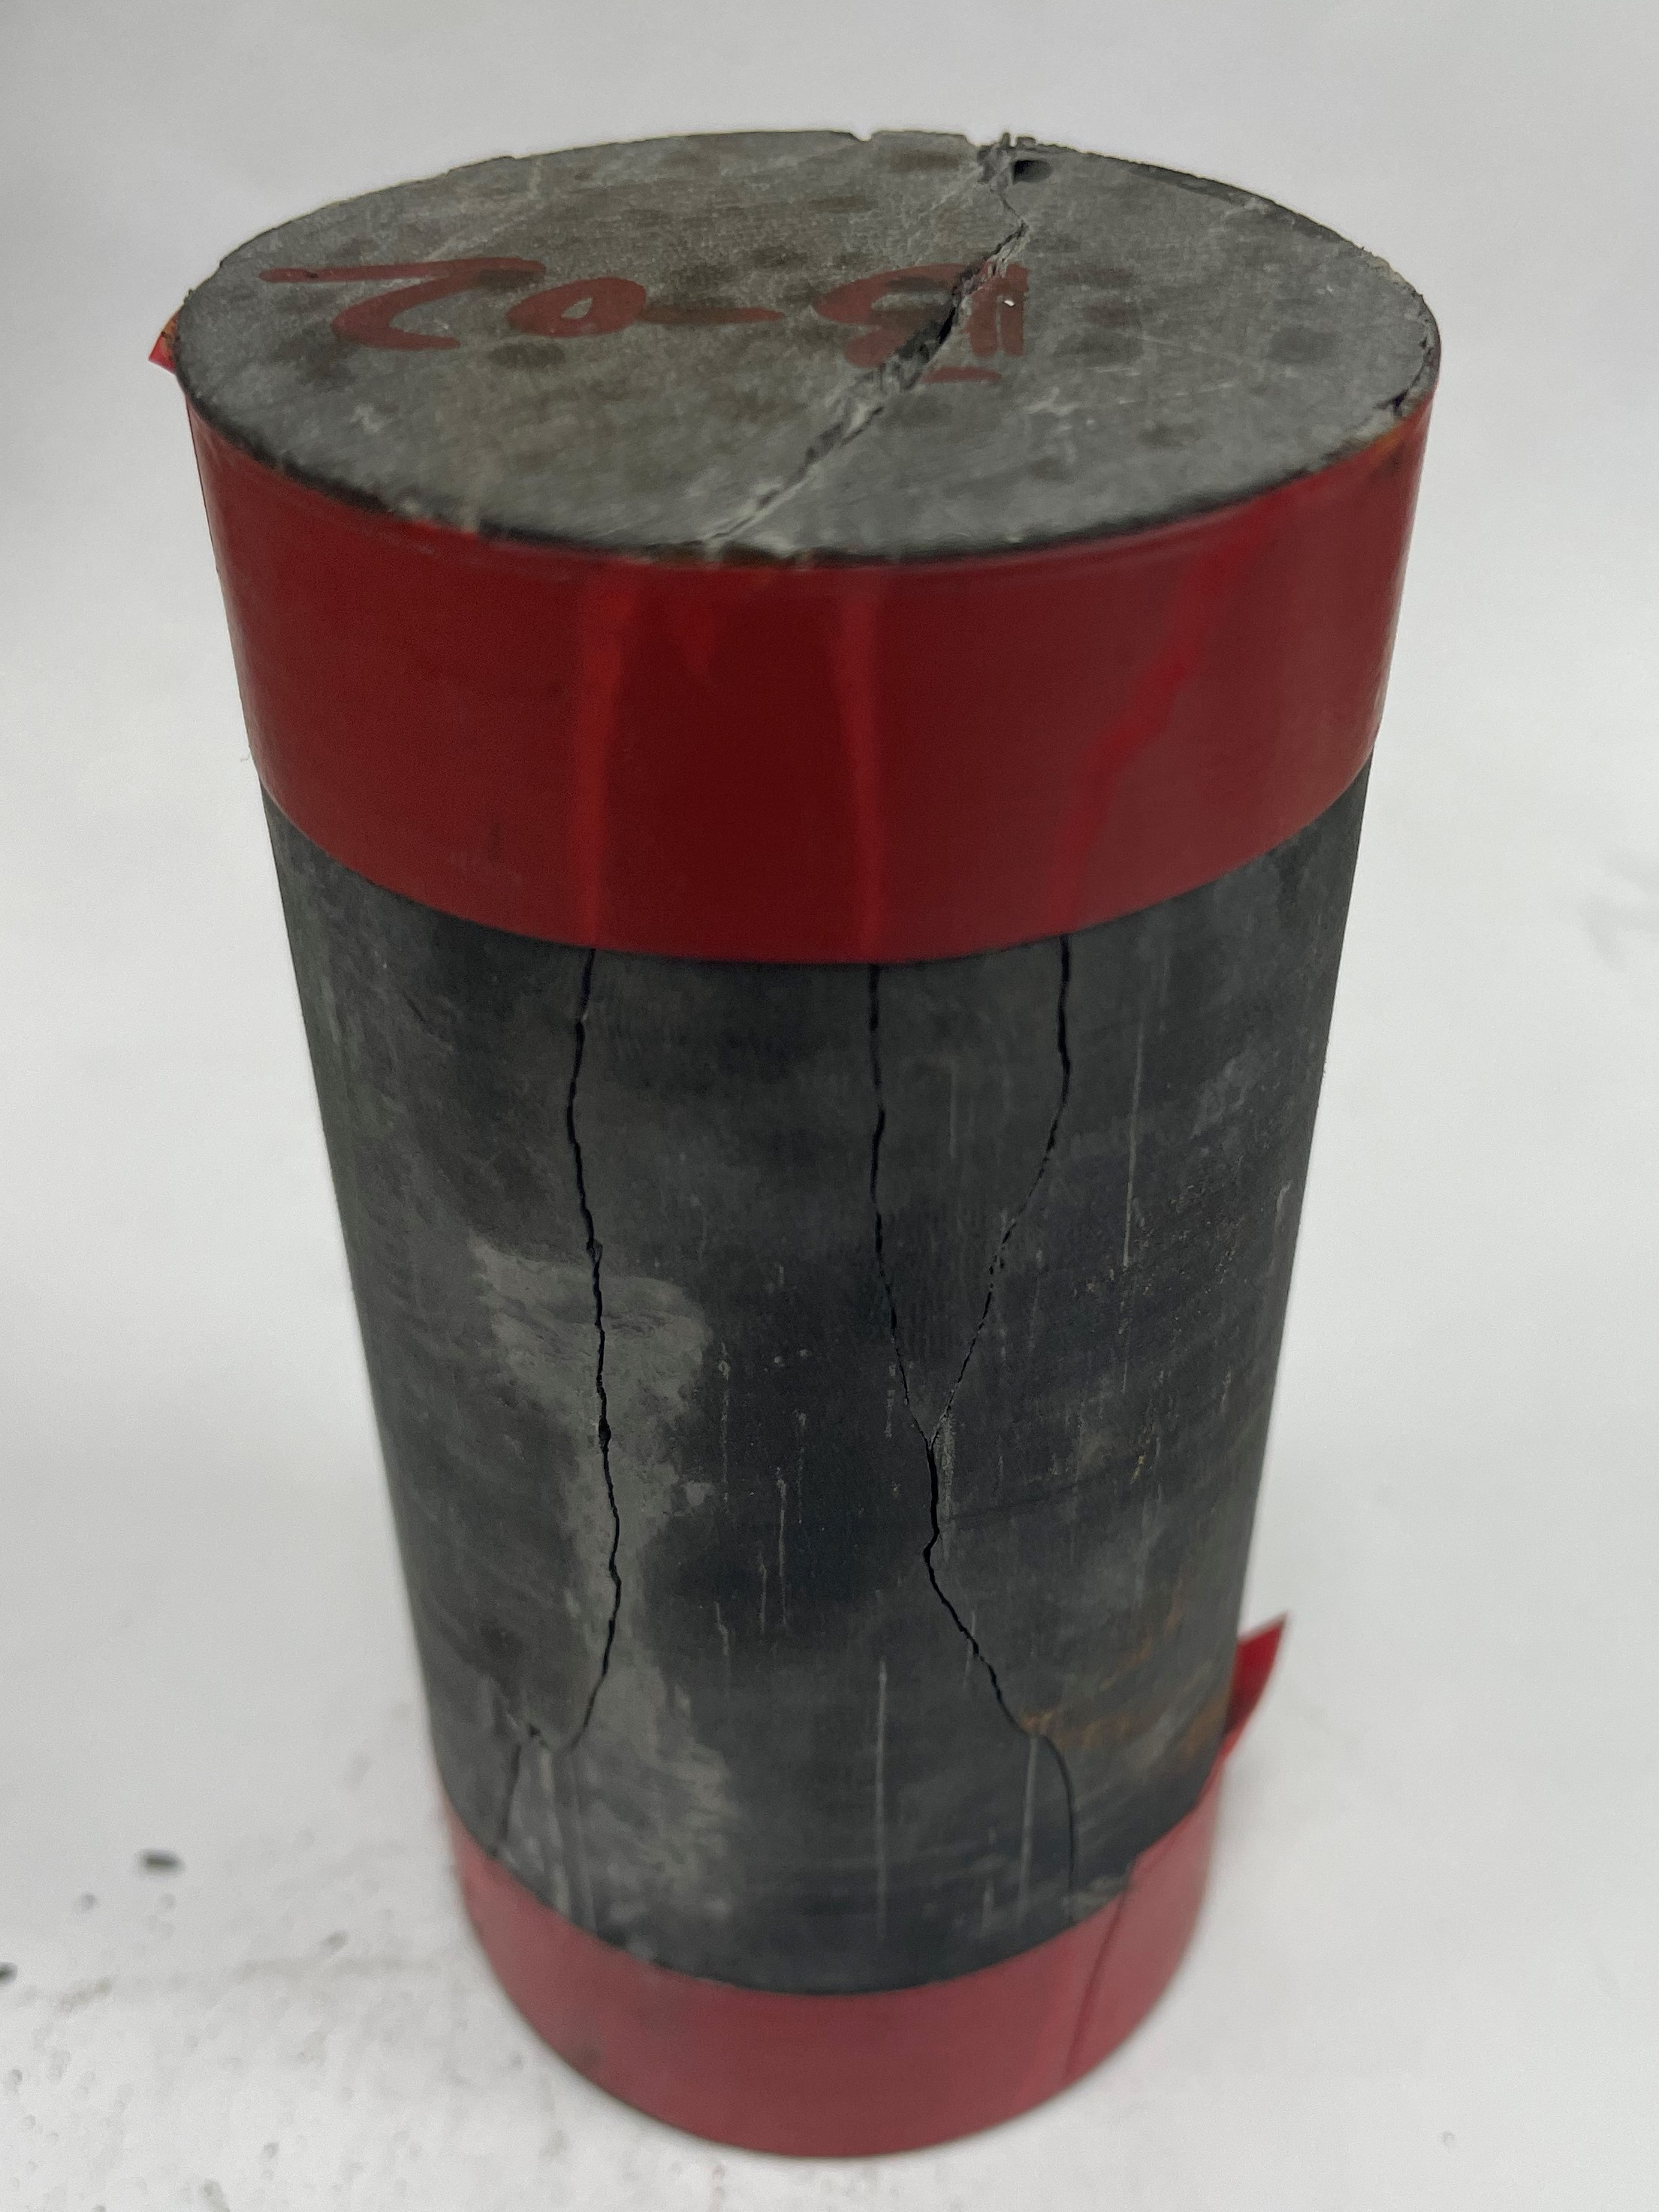
\includegraphics[width=0.9\textwidth]{img/chap2/B-02.jpg}
        \end{minipage}
    }
    \caption{试验步骤}
    \label{fig:2-4}
\end{figure}

由图中可以看出,砂质泥岩在三轴压缩破坏之后并没有表现出如硬岩般的破碎特
征,仍然保持较为完整的圆柱体形状。单轴压缩的试样,如A-01,其整体表现出的破坏形式为张拉破坏,局部出现裂缝,而三轴压缩下的B-02试样,裂缝贯穿整个试件,主要表现为剪切破坏。


\subsection{试样应力-应变曲线分析}
泥岩试样在不同围压下进行常规三轴压缩试验所得的应力-应变曲线如图~\ref{fig:2-4}所示。由图中的($\sigma_1$-$\sigma_3$)\textasciitilde $\varepsilon_1$关系曲线可以看
出,在试验初期阶段,试样在较低的轴压和围压的共同作用下已经完成了压密过程,处于弹性状态。通过图中曲线可以很明显地看出单轴压缩条件下的试样,最终的抗压强度远小于三轴压缩下的试样,单轴压缩条件下,试样在峰值强度附近已经出现了明显的屈服平台,表现出明显的脆性和应变软化特征。三轴压缩条件下,随着围压的增大,曲线弹性阶段的斜率也逐渐增大,极限承载能力和弹性模量也逐渐增大。

\begin{figure}[ht!]
    \centering
    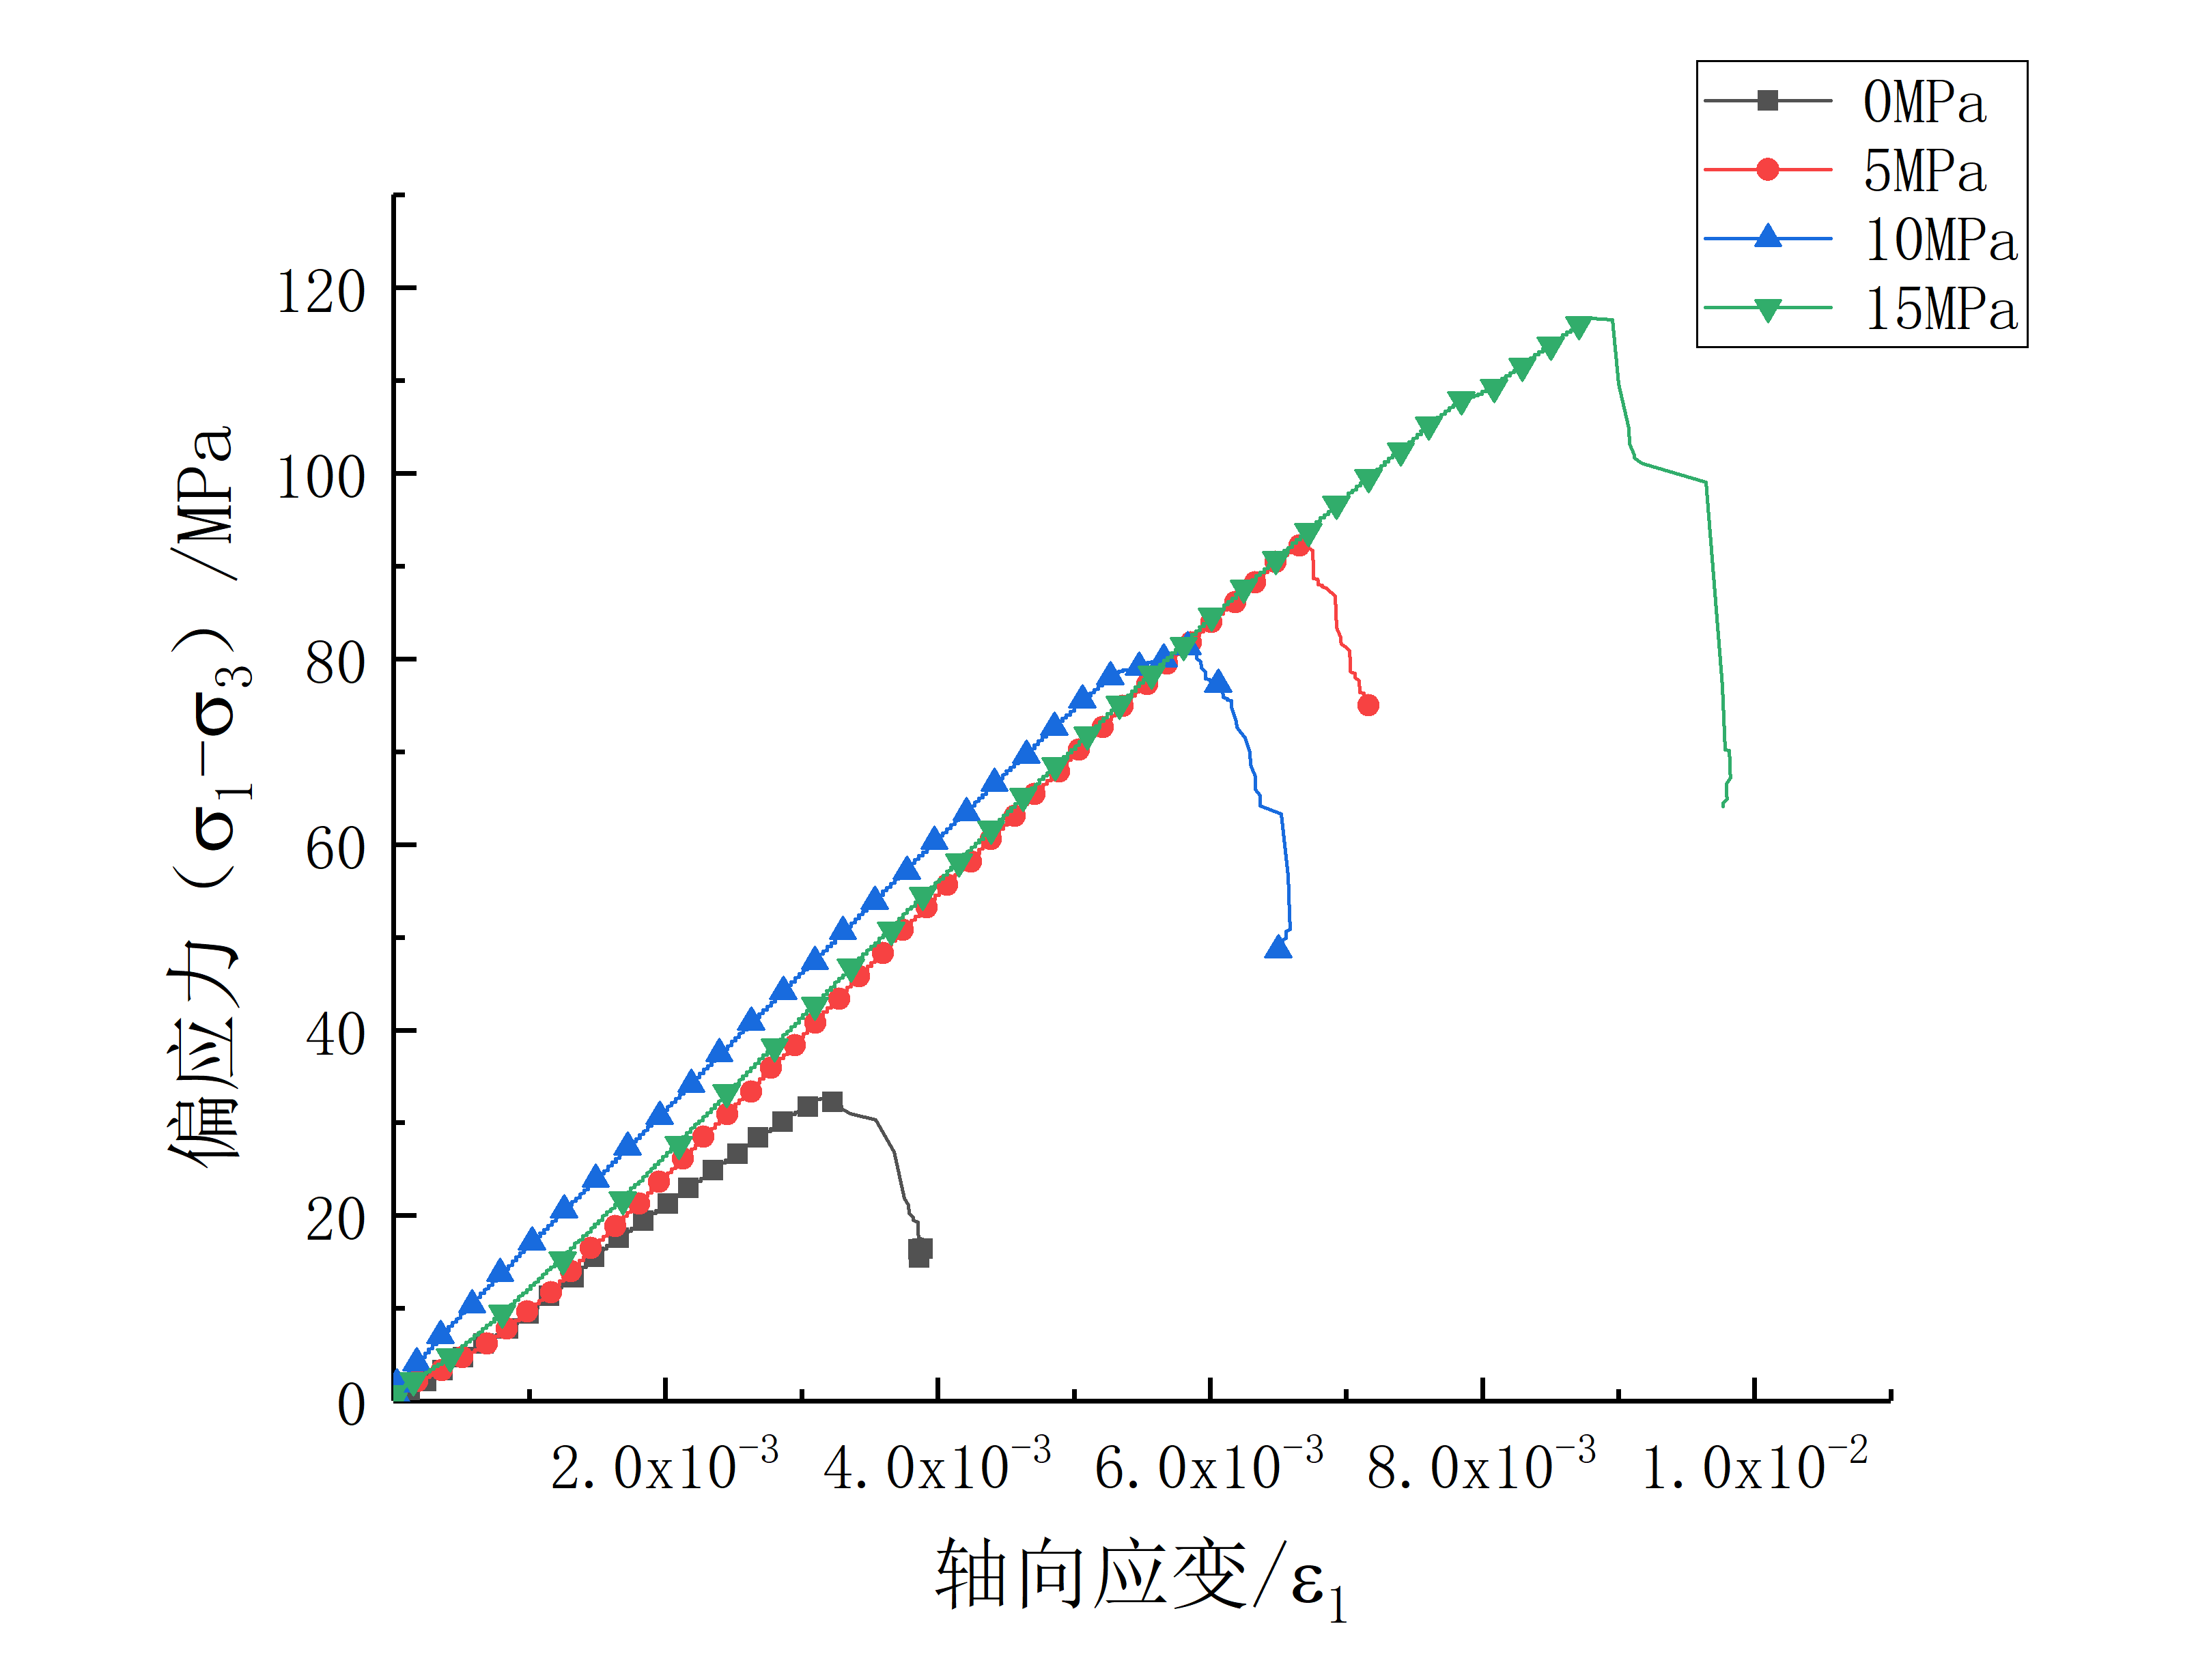
\includegraphics[width=0.7\textwidth]{img/chap2/2-4.png}
    \caption{泥岩三轴压缩应力-应变曲线}
    \label{fig:2-5}
\end{figure}

结合图2.4进行分析,整个试验过程的应力-应变曲线大致分为三个阶段:

(1)弹性变形阶段:该阶段应力一应变曲线呈直线关系,不仅意味着应变随应力成比例的增加,还表现为弹性变形的可恢复。曲线图中弹性阶段直线部分的斜率即为该岩石试样的弹性模量;

(2)微裂隙发展阶段:该阶段岩体中微裂隙开始产生、扩展、累积,新出现的裂纹随着应力的增大而不断发展,岩石产生不可逆变形,即产生相当部分的塑性变形,该阶段的上界称为屈服极限。当微裂隙稳定发展到一定程度后,会进入不稳定发展的状态,在这个过程中,试样薄弱处出现破坏,应力重分布后转嫁至次薄弱部位,次薄弱部位继续破坏直至试样完全破坏。在图~\ref{fig:2-4}中,该阶段表现不太明显,不过图中\SI{10}{MPa}和\SI{15}{MPa}的曲线在弹性阶段和曲线下降段之间可以看到一段与线性变化的直线不同的曲线段。本阶段的上界应力称为峰值强度;

(3)破裂后阶段:岩块达峰值后,内部结构破坏,但整体状态仍旧基本保持,岩样受力主要依靠裂隙面的摩擦力承担。到本阶段,裂隙快速发展,交叉且相互联合形成宏观断裂面试件承载力随变形增大迅速下降,但并不降到零,说明破裂的岩石仍有一定的承载力。

根据试验得到岩石的抗压强度,计算岩石弹性模量,计算公式如下:
\begin{equation}
    E=\frac{\sigma_b-\sigma_a}{\varepsilon_b-\varepsilon_a}
\end{equation}
\begin{shizhong}
     \item $\sigma_a$——应力—应变曲线弹性阶段应力峰值的30\%
     \item $\sigma_b$——应力—应变曲线弹性阶段应力峰值的50\%
     \item $\varepsilon_a$——应力为$\sigma_a$时的轴向应变值     
     \item $\varepsilon_b$——应力为$\sigma_b$时的轴向应变值
\end{shizhong}
 
经整理得岩石单轴压缩试验结果如表\ref{tab:泥岩单、三轴试验结果}所示。单轴压缩条件下,泥岩的峰值强度均值为\SI{28.13}{MPa},弹性模量为\SI{12.927}{GPa};而在三轴压缩的条件下,该种泥岩试样的抗压峰值强度大大提升,其均值约为\SI{96.80}{MPa},弹性模量为\SI{14.873}{GPa},由此可见围压对泥岩的强度和刚度都有较大影响。
\begin{table}[ht!]\small
    \centering
    \begin{tabular}{p{3cm}<{\centering} p{3cm}<{\centering} p{3cm}<{\centering} p{3cm}<{\centering}}
        \toprule
        试样编号  & 峰值强度/MPa  &  峰值应变   &  弹性模量/GPa\\
        \midrule
        A-01        & 32.75  &   0.0032  &  12.873   \\ 
        A-02        & 26.03 &   0.0027  &  13.906   \\ 
        A-03        & 25.61  &   0.0028  &  12.003  \\ 
        \midrule
        B-01        & 92.35  &   0.0067  &  15.330   \\ 
        B-02        & 81.32 &   0.0058 &  14.626   \\ 
        B-03        & 116.74 &   0.0088  &  14.679 \\ 
        \bottomrule
    \end{tabular}
    \caption{泥岩单、三轴试验结果}
    \label{tab:泥岩单、三轴试验结果}
\end{table}

    
在本次试验获得的曲线中,有两个阶段受试验环境的影响,在图中没有明显表示:一是在弹性阶段开始前,试样受到轴压和围压共同作用所导致的空隙压密阶段,在此阶段,岩石中原有的空隙在较低的轴压和围压共同作用下逐渐闭合,岩石被压密,形成初始非线性变形;二是在试件破坏后达到的塑性流动阶段,随着塑性变形的持续发展,最终强度不再降低,这是由于所用的刚性三轴压缩仪所设定的试样破坏即停止试验,没有继续对破坏的试件施加轴向应力,所以没有塑性流动阶段的试验记录。


\section{泥岩单轴流变试验}\label{section:泥岩单轴流变试验}
\subsection{流变试验过程}
常规室内岩石蠕变试验的加载方式一般有三种,分别是分别加载、分级加载以及分级加卸载。分别加载法是用同种岩样制成一组试样,在相同的试验条件下对每个试样施加不
同的恒定荷载,观察同一组试样在不同加载应力下的流变过程。该方法能够使试样避免受到加载状态和加载历史的影响,蠕变曲线可以不经处理直接应用,实验结果理想可靠。然而,每个试样性质很难完全一致导致试验结果离散性较大,并且所需试验设备数量较多会使得试验成本过高,一般实验室难以满足。

分级加载法是在同一试样上逐级施加荷载,在一级荷载施加后,岩样经历给定的
的蠕变趋于稳定或达到预期时,再施加下一级荷载。该方法可在同一试样上获得更多的试验资料,结果离散性较小,可以减少试验操作过程中产生的误差。其缺点是试样在各级荷载下的变形相互交叉影响,该方法所得蠕变曲线为阶梯状,直接应用较少,需对蠕变曲线经过处理后才方便应用。

分级加卸载是指在一个试样上施加一定荷载,在荷载作用下变形基本稳定后卸除荷载,当滞后弹性变形恢复稳定(不增长),再在同一试样上进行下一级荷载的循环,直至试样加载到预设的应力等级或试样破坏,它吸收了分级加载法的优点,又在理论上避免了各级荷载下的变形相互影响。但在实际过程中,频繁的加卸载会导致岩石的性质发生改变。

通过对规格为直径\SI{50}{mm},高为\SI{100}{mm}的标准圆柱体的5个泥岩试样进行单轴流变试验,观察在常温下,岩石流变破坏所需的时间。
将试样标号为$C-01$、$C-02$、$C-03$、$C-04$、$C-05$,根据岩石单轴压缩试验确定岩石变形破坏最基本的力学特
性及参数,合理地选取加载应力水平进行流变试验,具体工况如表~\ref{tab:泥岩单轴流变试验工况表}所示:

\begin{table}[ht!]\small
    \centering
    \begin{tabular}{p{3cm}<{\centering} p{3cm}<{\centering} p{3cm}<{\centering} p{3cm}<{\centering}}
        \toprule
        试样编号  & 围压(MPa)  &  加载强度(MPa)   &  加载时间(h)\\
        \midrule
        C-01        & 0  &   26.3  &     \\ 
        C-02        & 0  &   24.8  &     \\ 
        C-03        & 0  &   23.4  &     加载至试样破坏\\
        C-04        & 0  &   22.0  &     \\
        C-05        & 0  &   20.5  &     \\
        \bottomrule
    \end{tabular}
    \caption{泥岩单轴流变试验工况表}
    \label{tab:泥岩单轴流变试验工况表}
\end{table}




由单轴压缩试验得岩石的强度,并以此为依据确定岩石单轴蠕变试验的加载等级。
在蠕变试验中我们所采用的仪器与上一小节三轴压缩试验使用的仪器为同一台,因此不再多做介绍。试验步骤依据~\ref{section:试验过程}节的基本方案对进行,具体实验过程如下所述:

(1)从试样选取与编号、试样安装到充油施加围压(单轴蠕变试验无须施加围压)这三步与2.2.1节中进行常规三轴压缩试验的前三步操作相同。

(2)在围压施加完成后,将试样与三轴伺服仪轴压压头进行接触,可手动操作向轴压压力室加油,待轴向应变变化说明已经接触,且接触后要卸载此时的偏应力值到零,最后加满轴压泵。

(3)而与三轴压缩试验不同的是,在蠕变实验中,我们采用应力加载方式,加载速度为\SI{3}{MPa/min}。由于采用的时分级加载的方式,根据试验前算得每一级偏应力,当轴压施加到预计值时,需要保持此时的偏应力一段时间,具体时间根据工况表中的预计加载时间以及试样实验时的实际情况确定,待达到预定加载时间后,再施加下一级应力。若试样在某一级加载中损坏,便结束试验并取出损坏的试样。


\subsection{流变特征分析}
研究表明,岩石除了在加载瞬间产生的瞬时变形,随后会发生缓慢且持续的蠕变变形,基于岩石的流变特性,岩石的流变曲线大致上如图~\ref{fig:2-8}所示。岩石蠕变过程一般分为三个阶段,分别是初始变阶段、稳定蠕变阶段和加速蠕变阶段的应变。在初始蠕变阶段,应变随时间增大,但应变增长的速率逐渐减小,因此该阶段也叫减速蠕变阶段;第二阶段是稳定蠕变阶段,岩石的蠕变速率在第一阶段末逐渐减小到一定值后保持不变,在这个阶段蠕变曲线近似直线,应变随时间的增长近似线性增加,蠕变变形最终趋于稳定;第三阶段为加速蠕变阶段,此时蠕变速率随时间迅速增大,岩石变形快速发展直至破坏。

\begin{figure}[ht!]
    \centering
        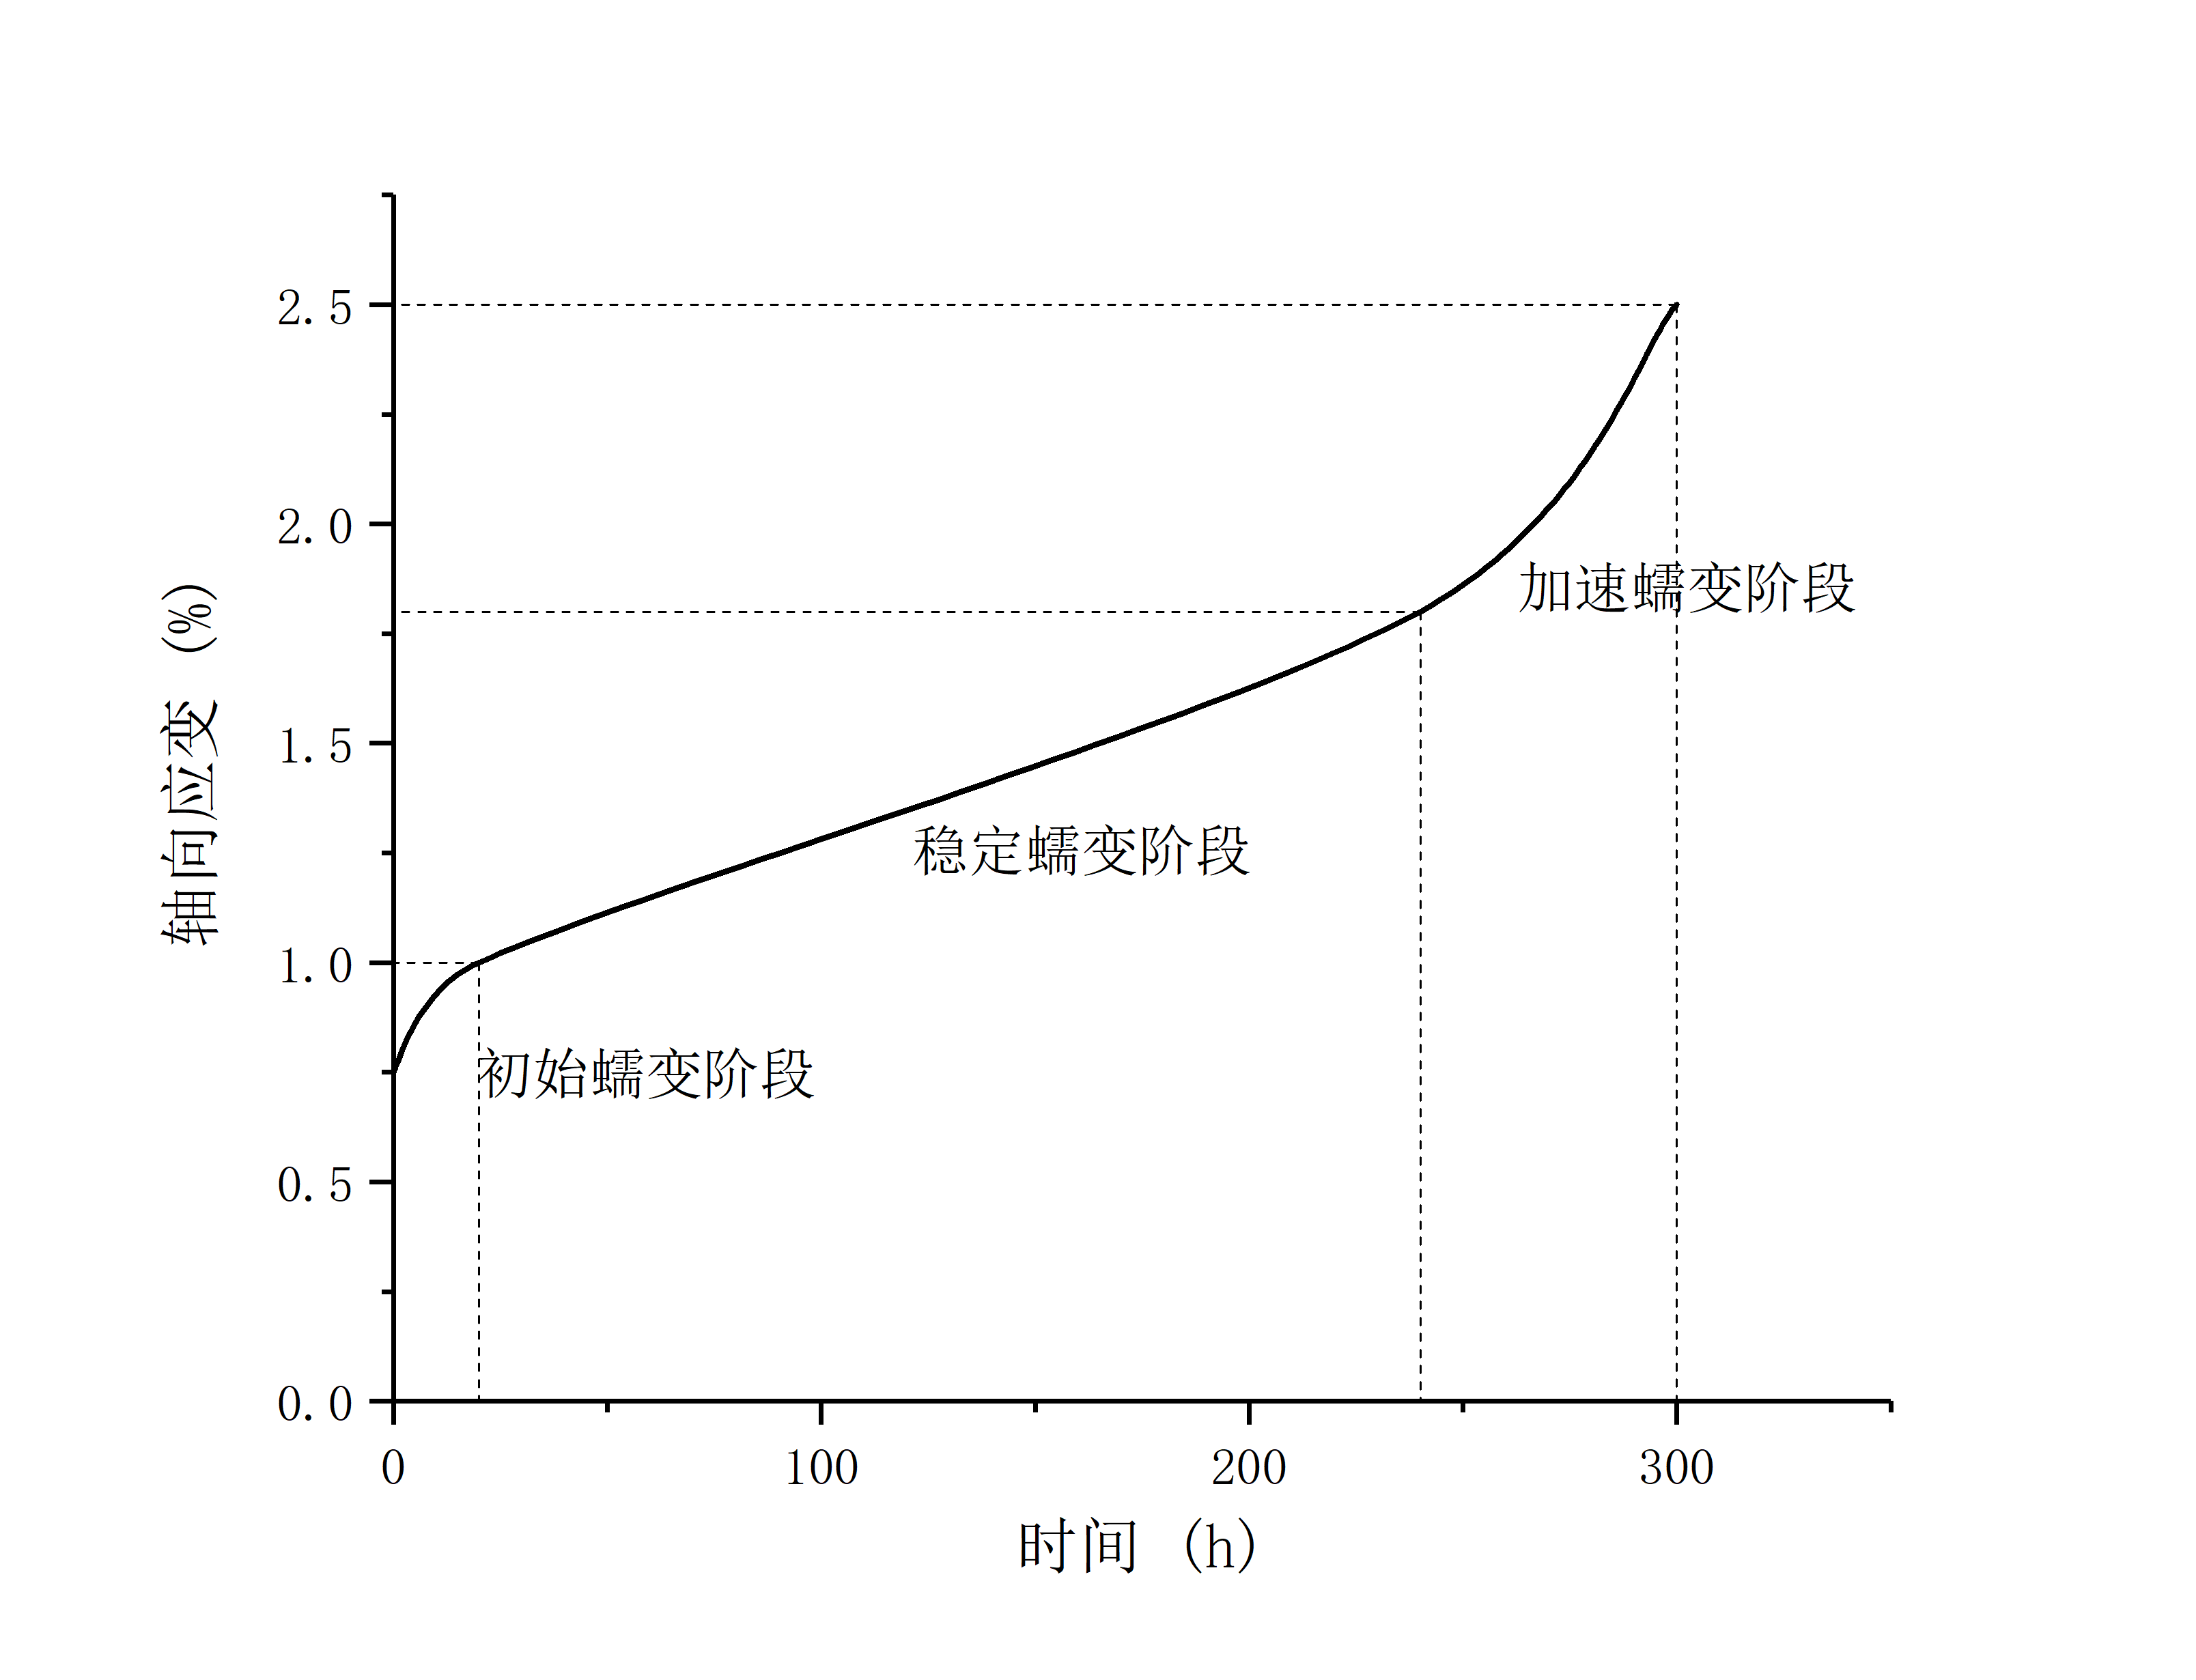
\includegraphics[width=0.7\textwidth]{img/chap2/Creep curve.png}
    \caption{蠕变曲线}
    \label{fig:2-8}
\end{figure}

\subsection{单轴流变曲线分析}

流变试验结束后,我们对收集到的实验数据进行集中处理,由此可以得到各个试样的流变数据曲线,进行分别加载的单轴压缩流变试验所得到曲线如图~\ref{fig:2-9}所示,我们可以发现:

(1)在我们所完成的5个单轴压缩流变试验中,试样在加载的瞬间都会产生瞬时压缩变形。并且根据试验工况表中的加载强度,结合试验数据来看,试样发生的瞬时轴向应变会随着加载强度的增大而增大。例如,在C-01试样中,加载到预定的强度等级后,瞬时应变达到了0.21\%,C-02的瞬时应变则为0.19\%。

(2)除 C-03 外,其余四组试验在产生瞬时变形后,其轴向应变仍会随时间的增长缓慢增加,说明试样进入了蠕变过程,进入蠕变阶段后,变形会随着时间增加,蠕变变形趋于稳定,故在图中看起来近似一条直线。而 C-03 试样在加载到预定应力等级的过程中也产生了瞬时轴向应变,不过从实验数据上看,在达到蠕变阶段不久,施加的偏应力迅速减小,轴向应变突然增大,试样进入加速蠕变阶段,此时试样已经破坏,可以认为在加载过程中岩样已经积累大量损伤,故不作为流变破坏讨论。

(3)从图(a)中可以看出,相比C-02、C-04、C-05,C-01在达到蠕变阶段后,轴向应变依旧有明显的上升。因此,在应力水平较高时,试样蠕变达到稳定后,轴向应变依旧会产生,在经历一定时间后流变变形量呈线性增长,流变变形速率趋于某一不为零的定值。而在较低的应力水平下,试样在达到蠕变后,蠕变速率会减小到接近于0,蠕变应变基本不再产生,这种情况下,整个试验的变形过程就是以试样的瞬时轴向应变和一小段的初始蠕变过程为主。

(4)在流变曲线中,试样在达到稳定流变阶段后,在某些时间节点上,轴向应变会突然上下波动,这是因为试样中存在着初始损伤,试样中的微小裂隙在偏应力作用下不断发展,造成局部破裂形成的,对流变过程产生了一定的影响,不过这种影响并不显著。

\begin{figure}[ht!]
    \centering
    \subfigure[C-01]
    {
        \begin{minipage}{7cm}
            \centering
            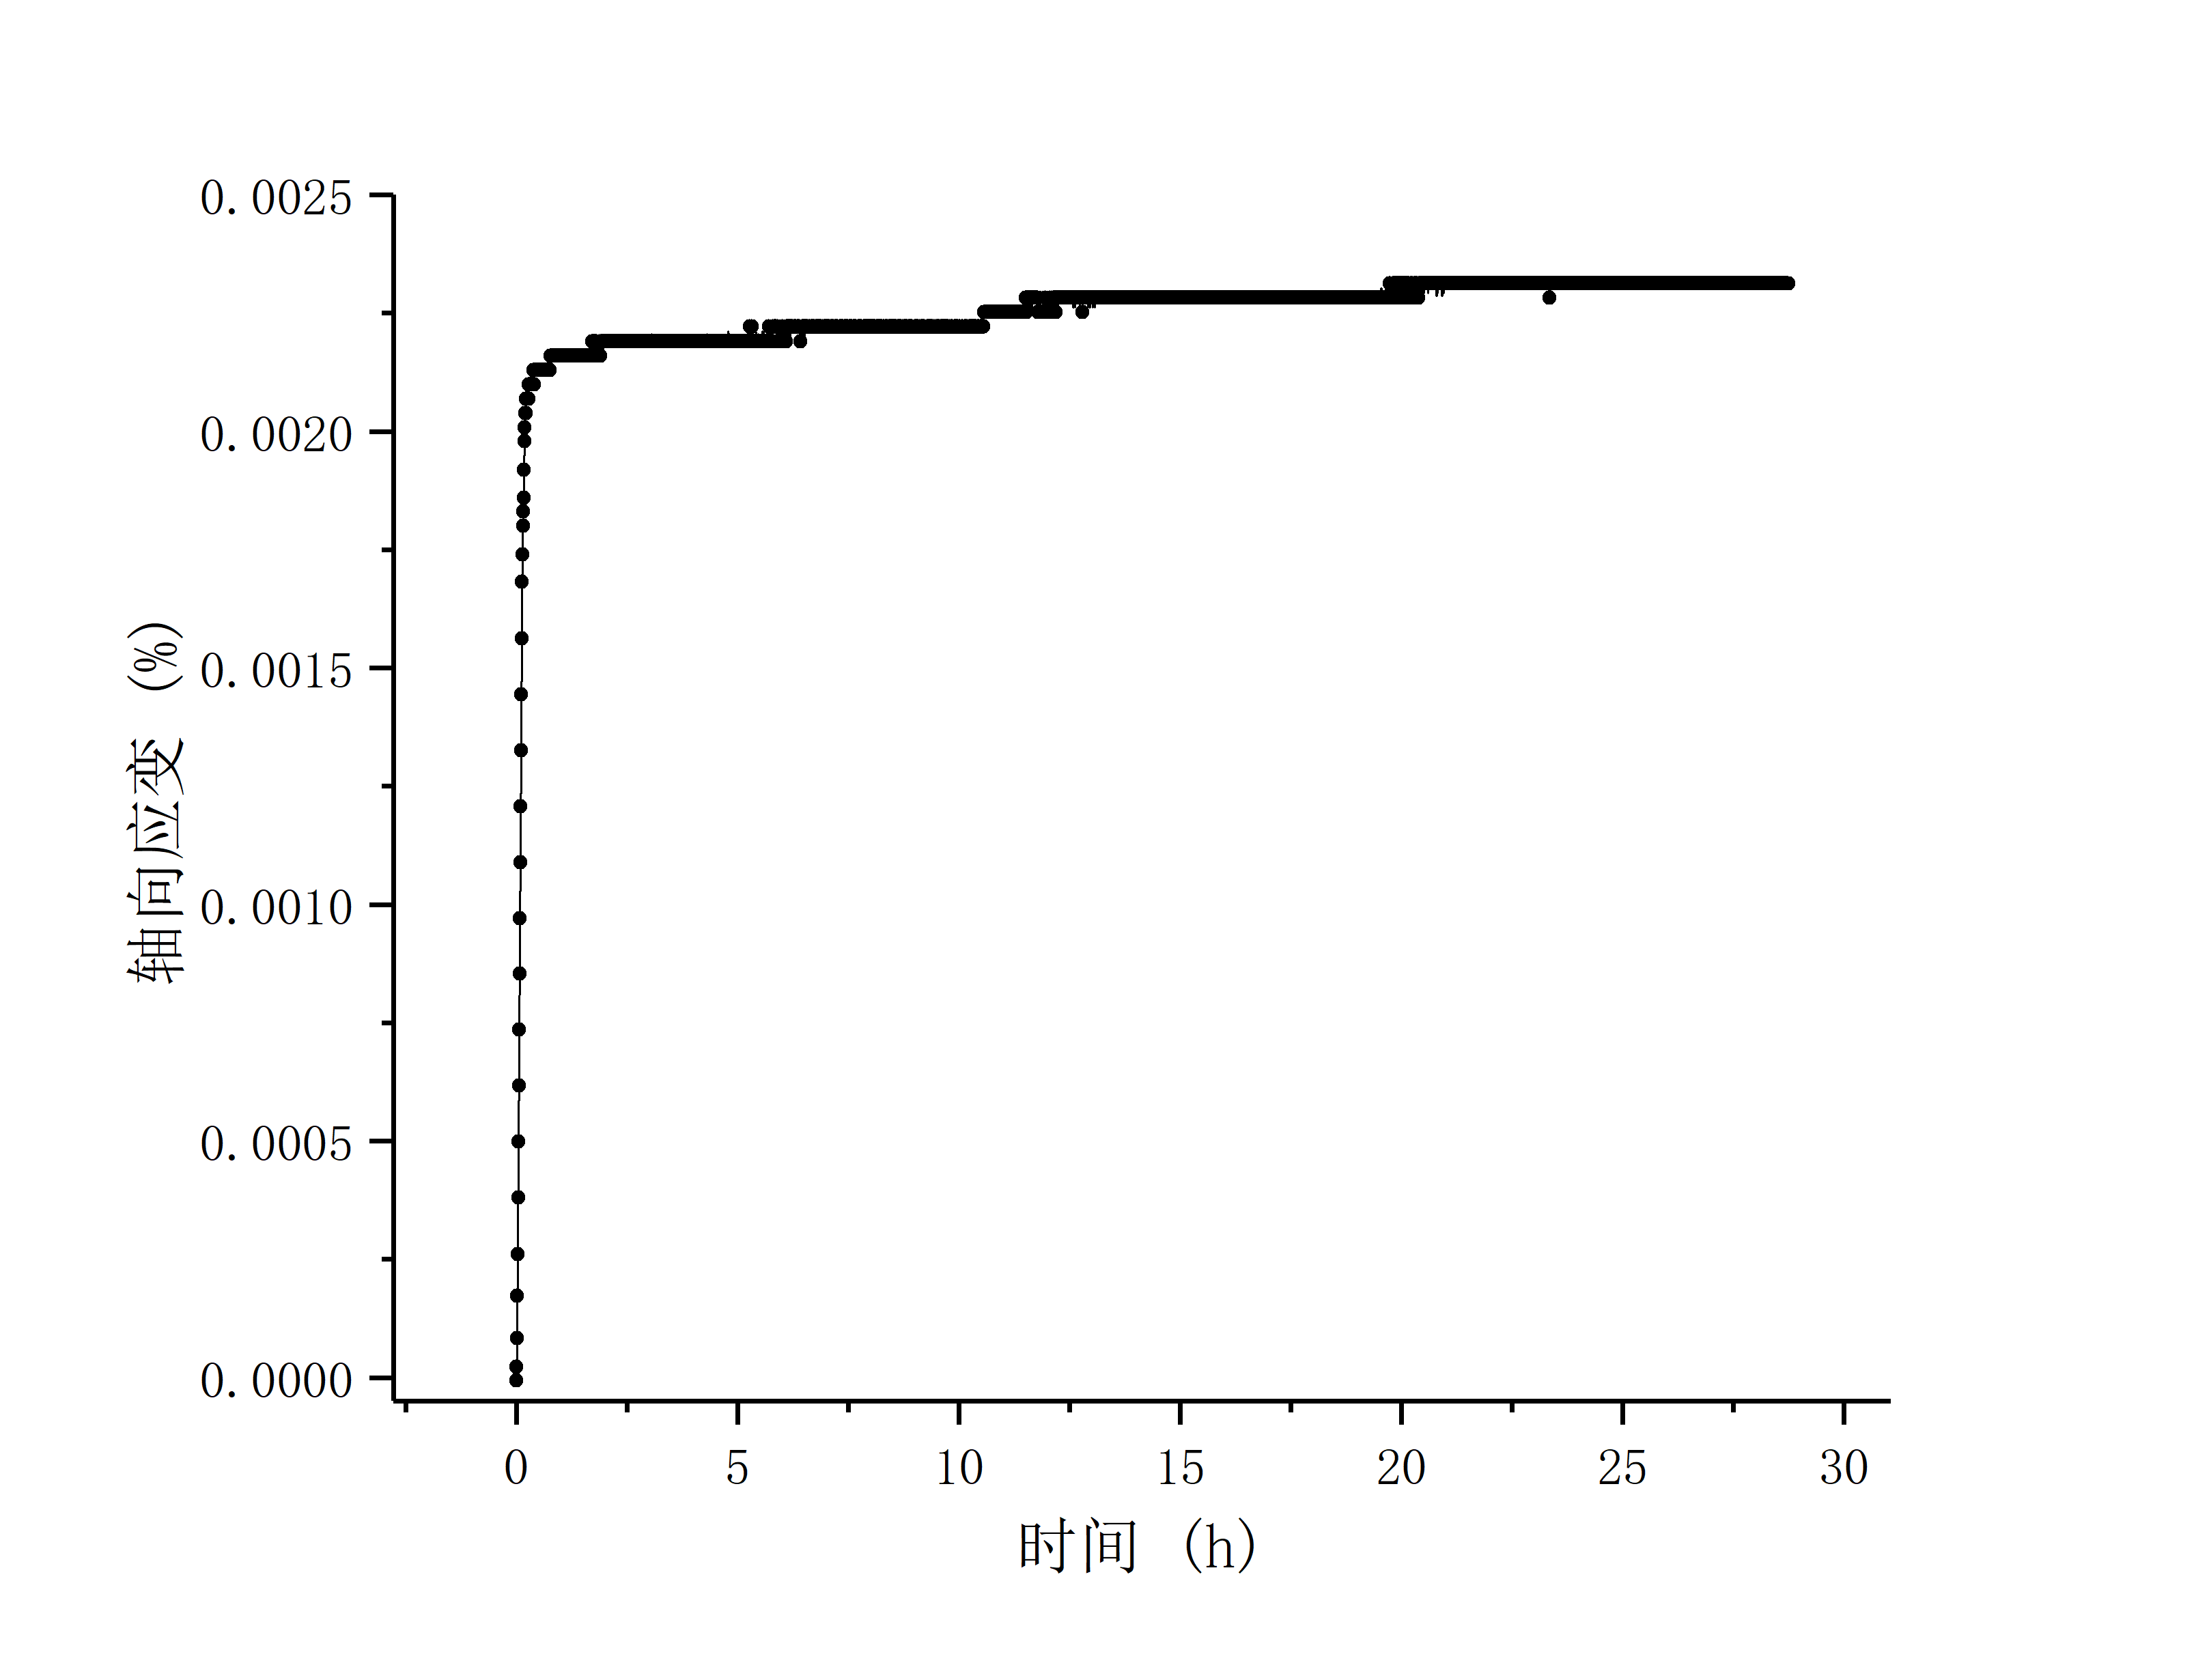
\includegraphics[width=1.1\textwidth]{img/chap2/C-01.png}
        \end{minipage}
    }
    \subfigure[C-02]
    {
        \begin{minipage}{7cm}
            \centering
            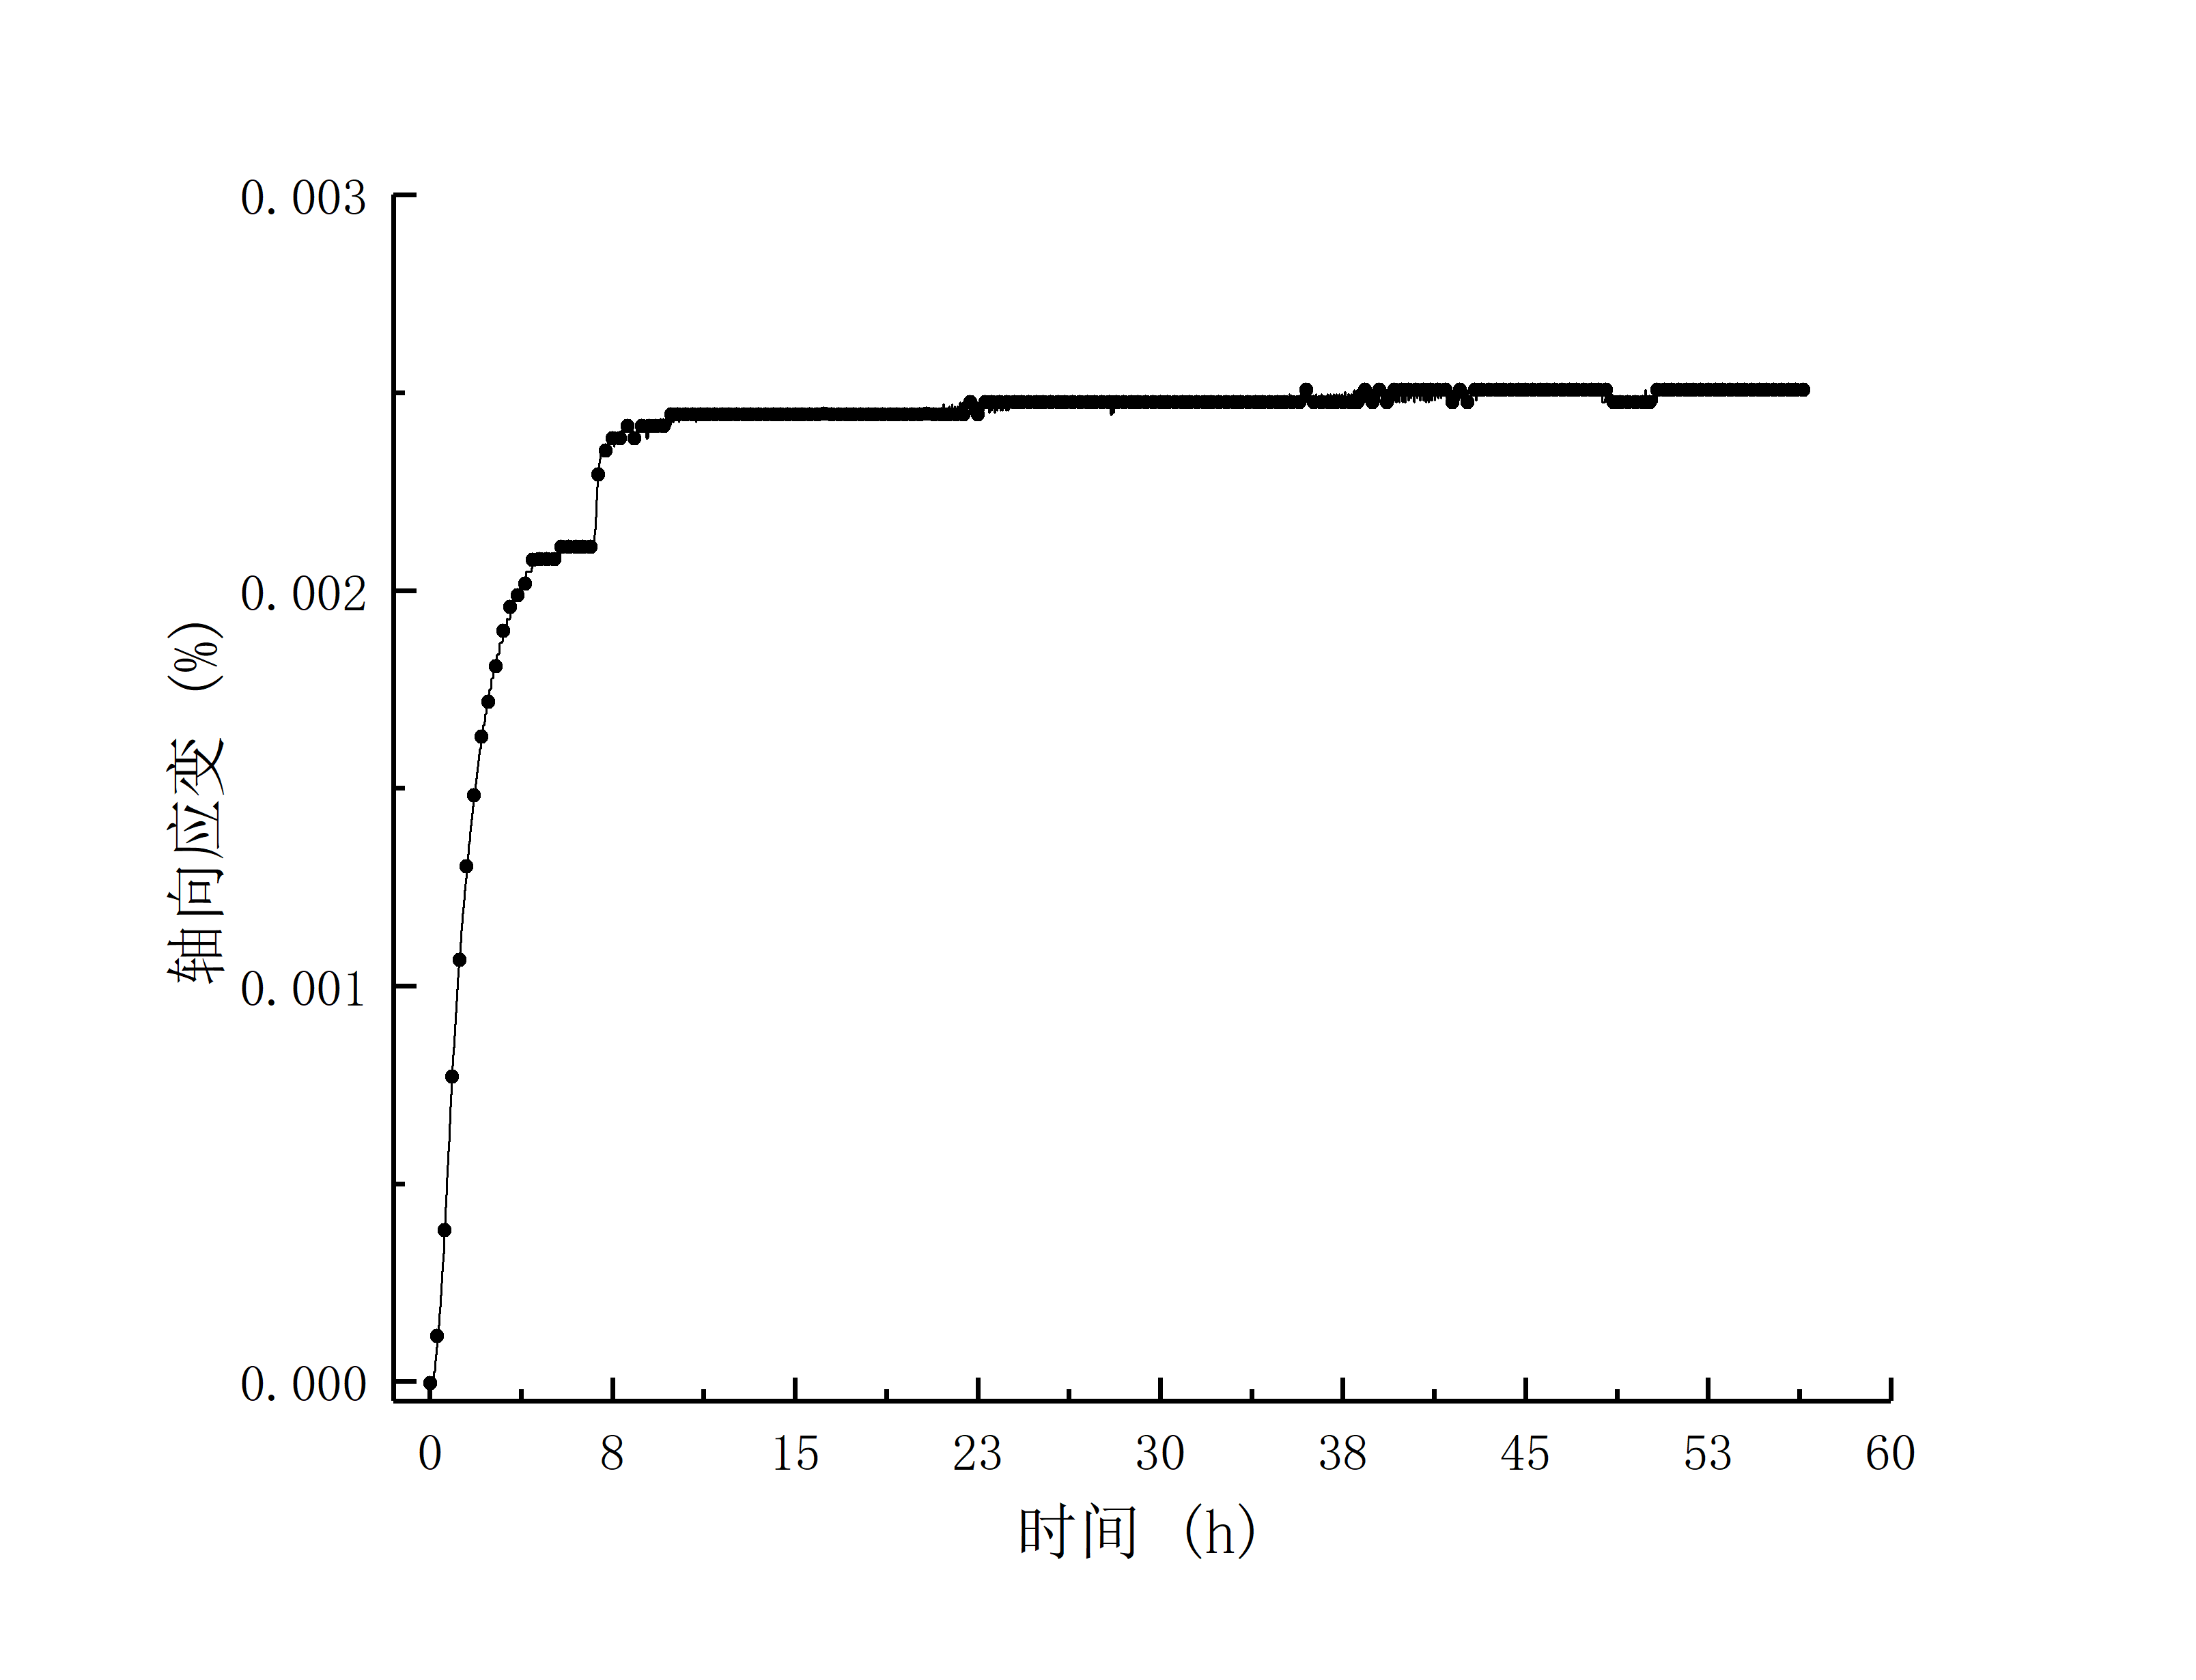
\includegraphics[width=1.1\textwidth]{img/chap2/C-02.png}
        \end{minipage}
    }
	
    \subfigure[C-03]
    {
        \begin{minipage}{7cm}
            \centering
            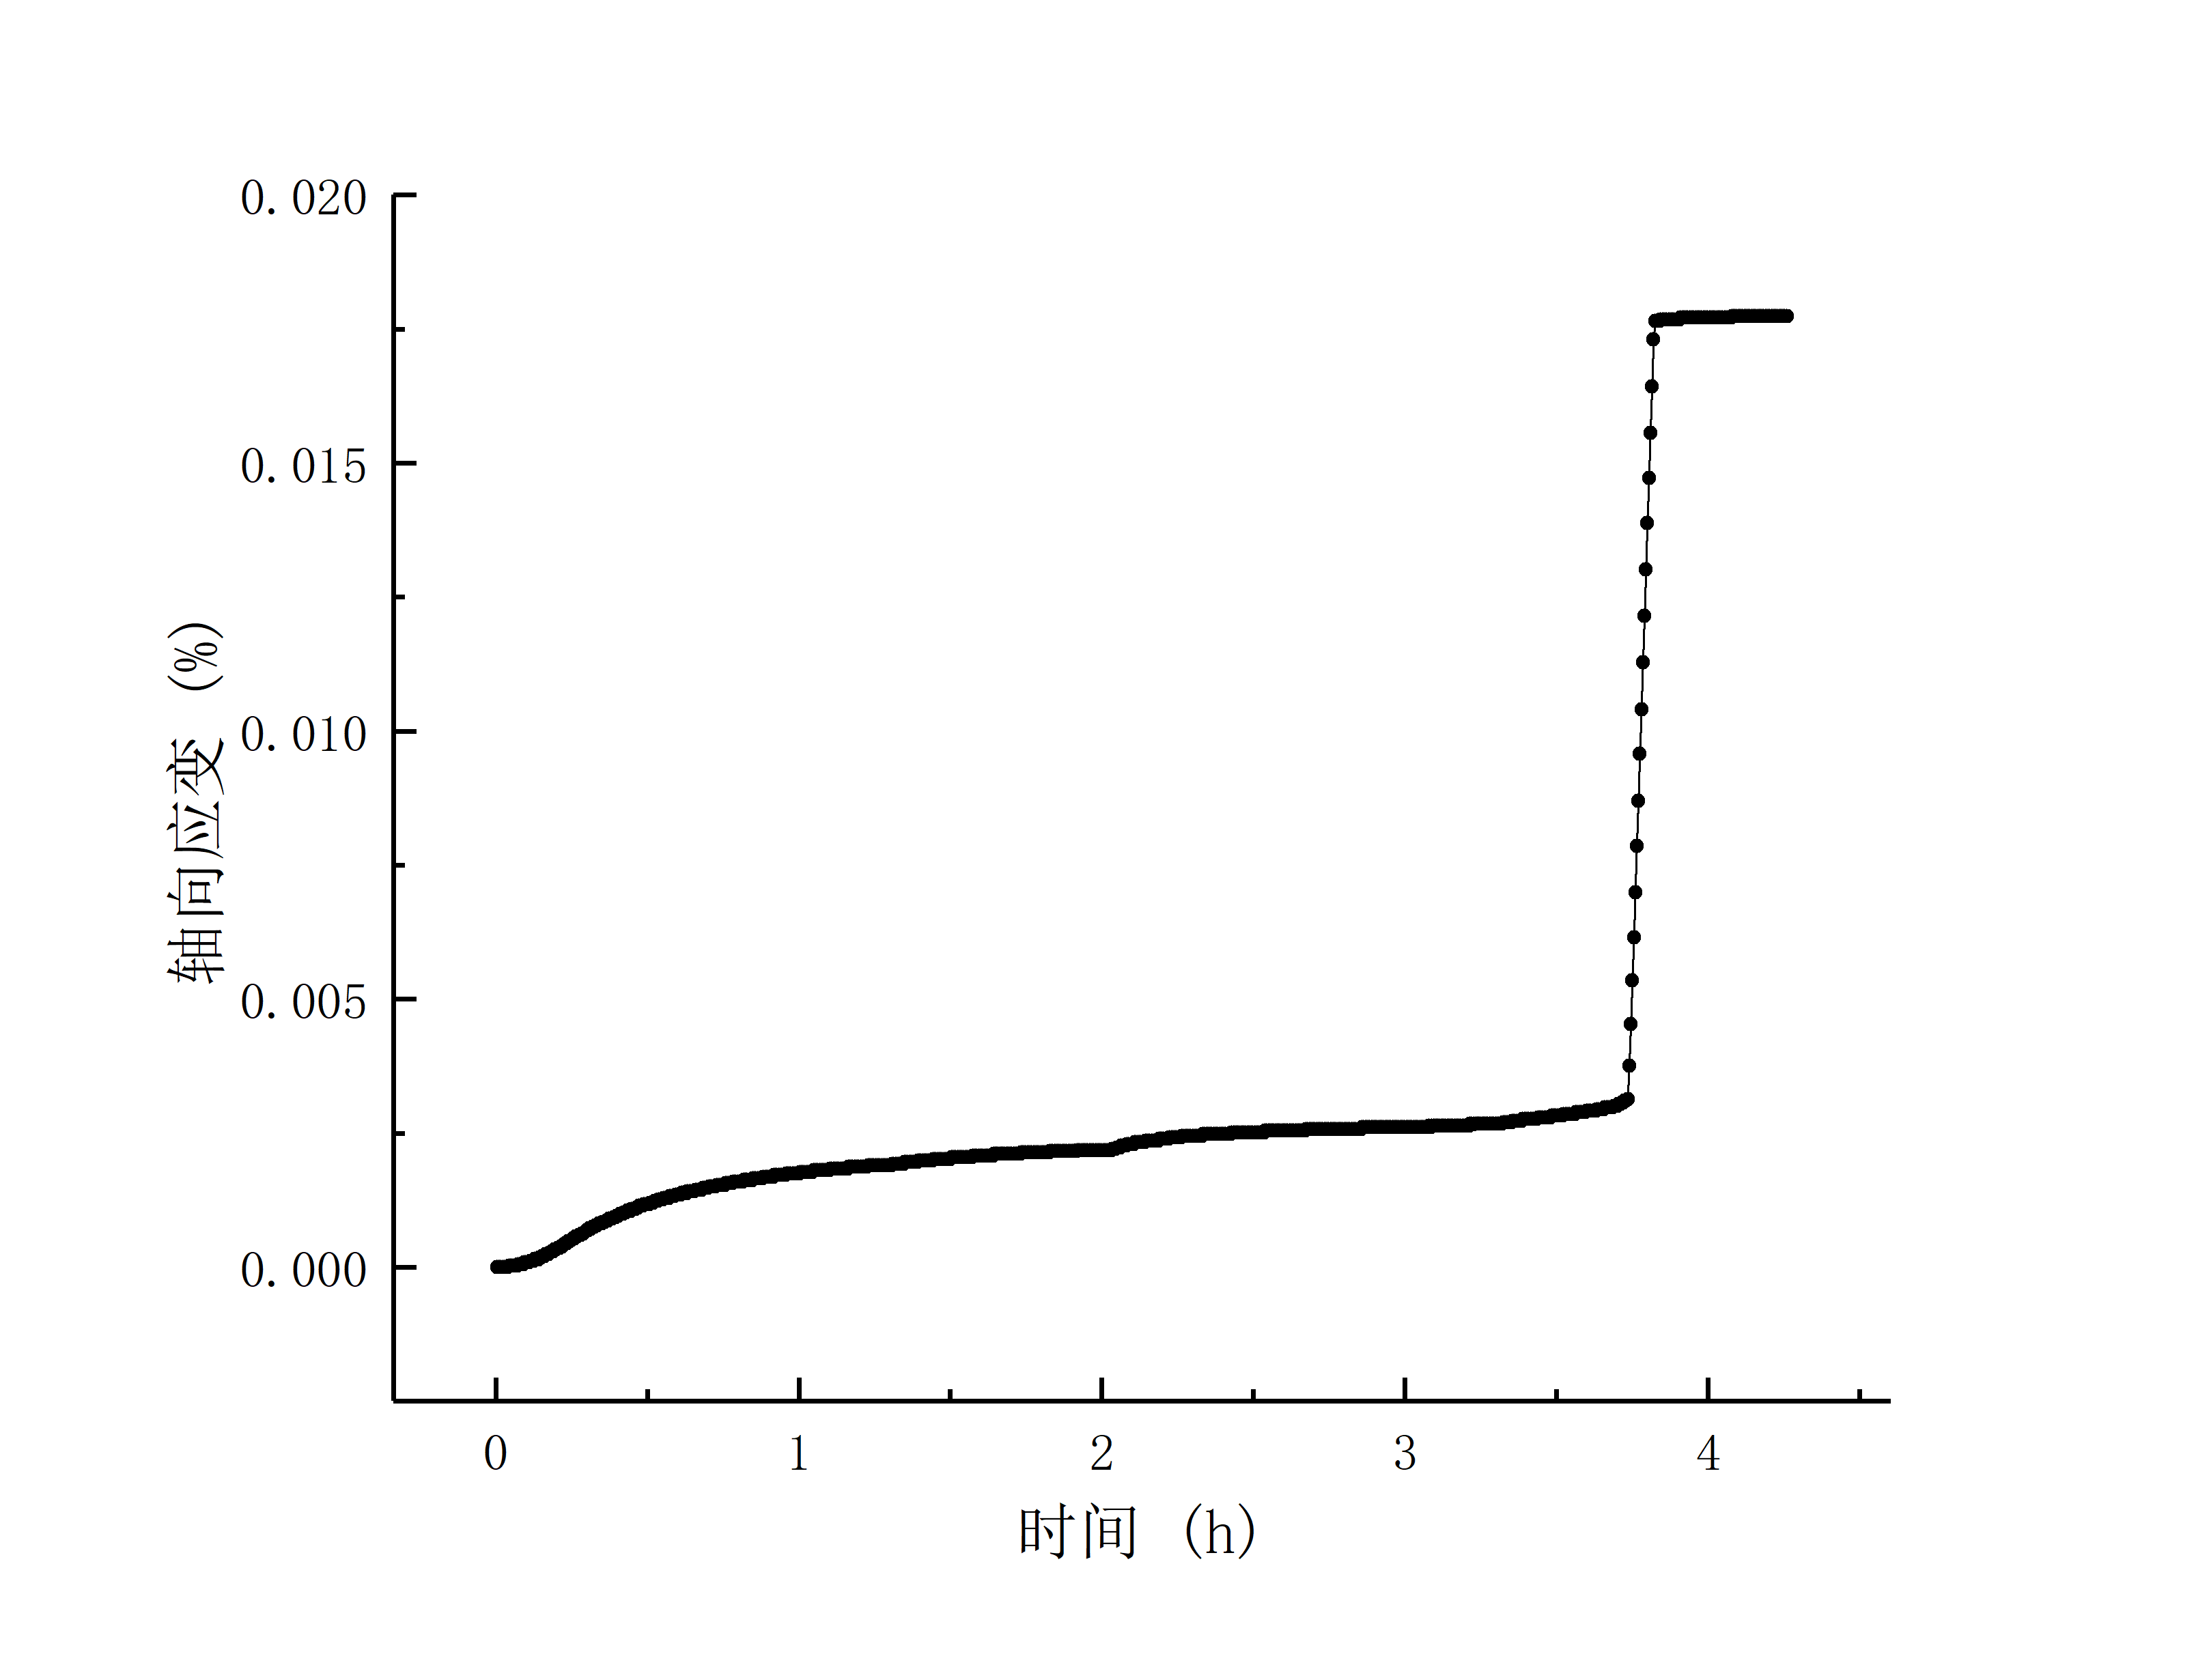
\includegraphics[width=1.1\textwidth]{img/chap2/C-03.png}
        \end{minipage}
    }
    \subfigure[C-04]
    {
        \begin{minipage}{7cm}
            \centering
            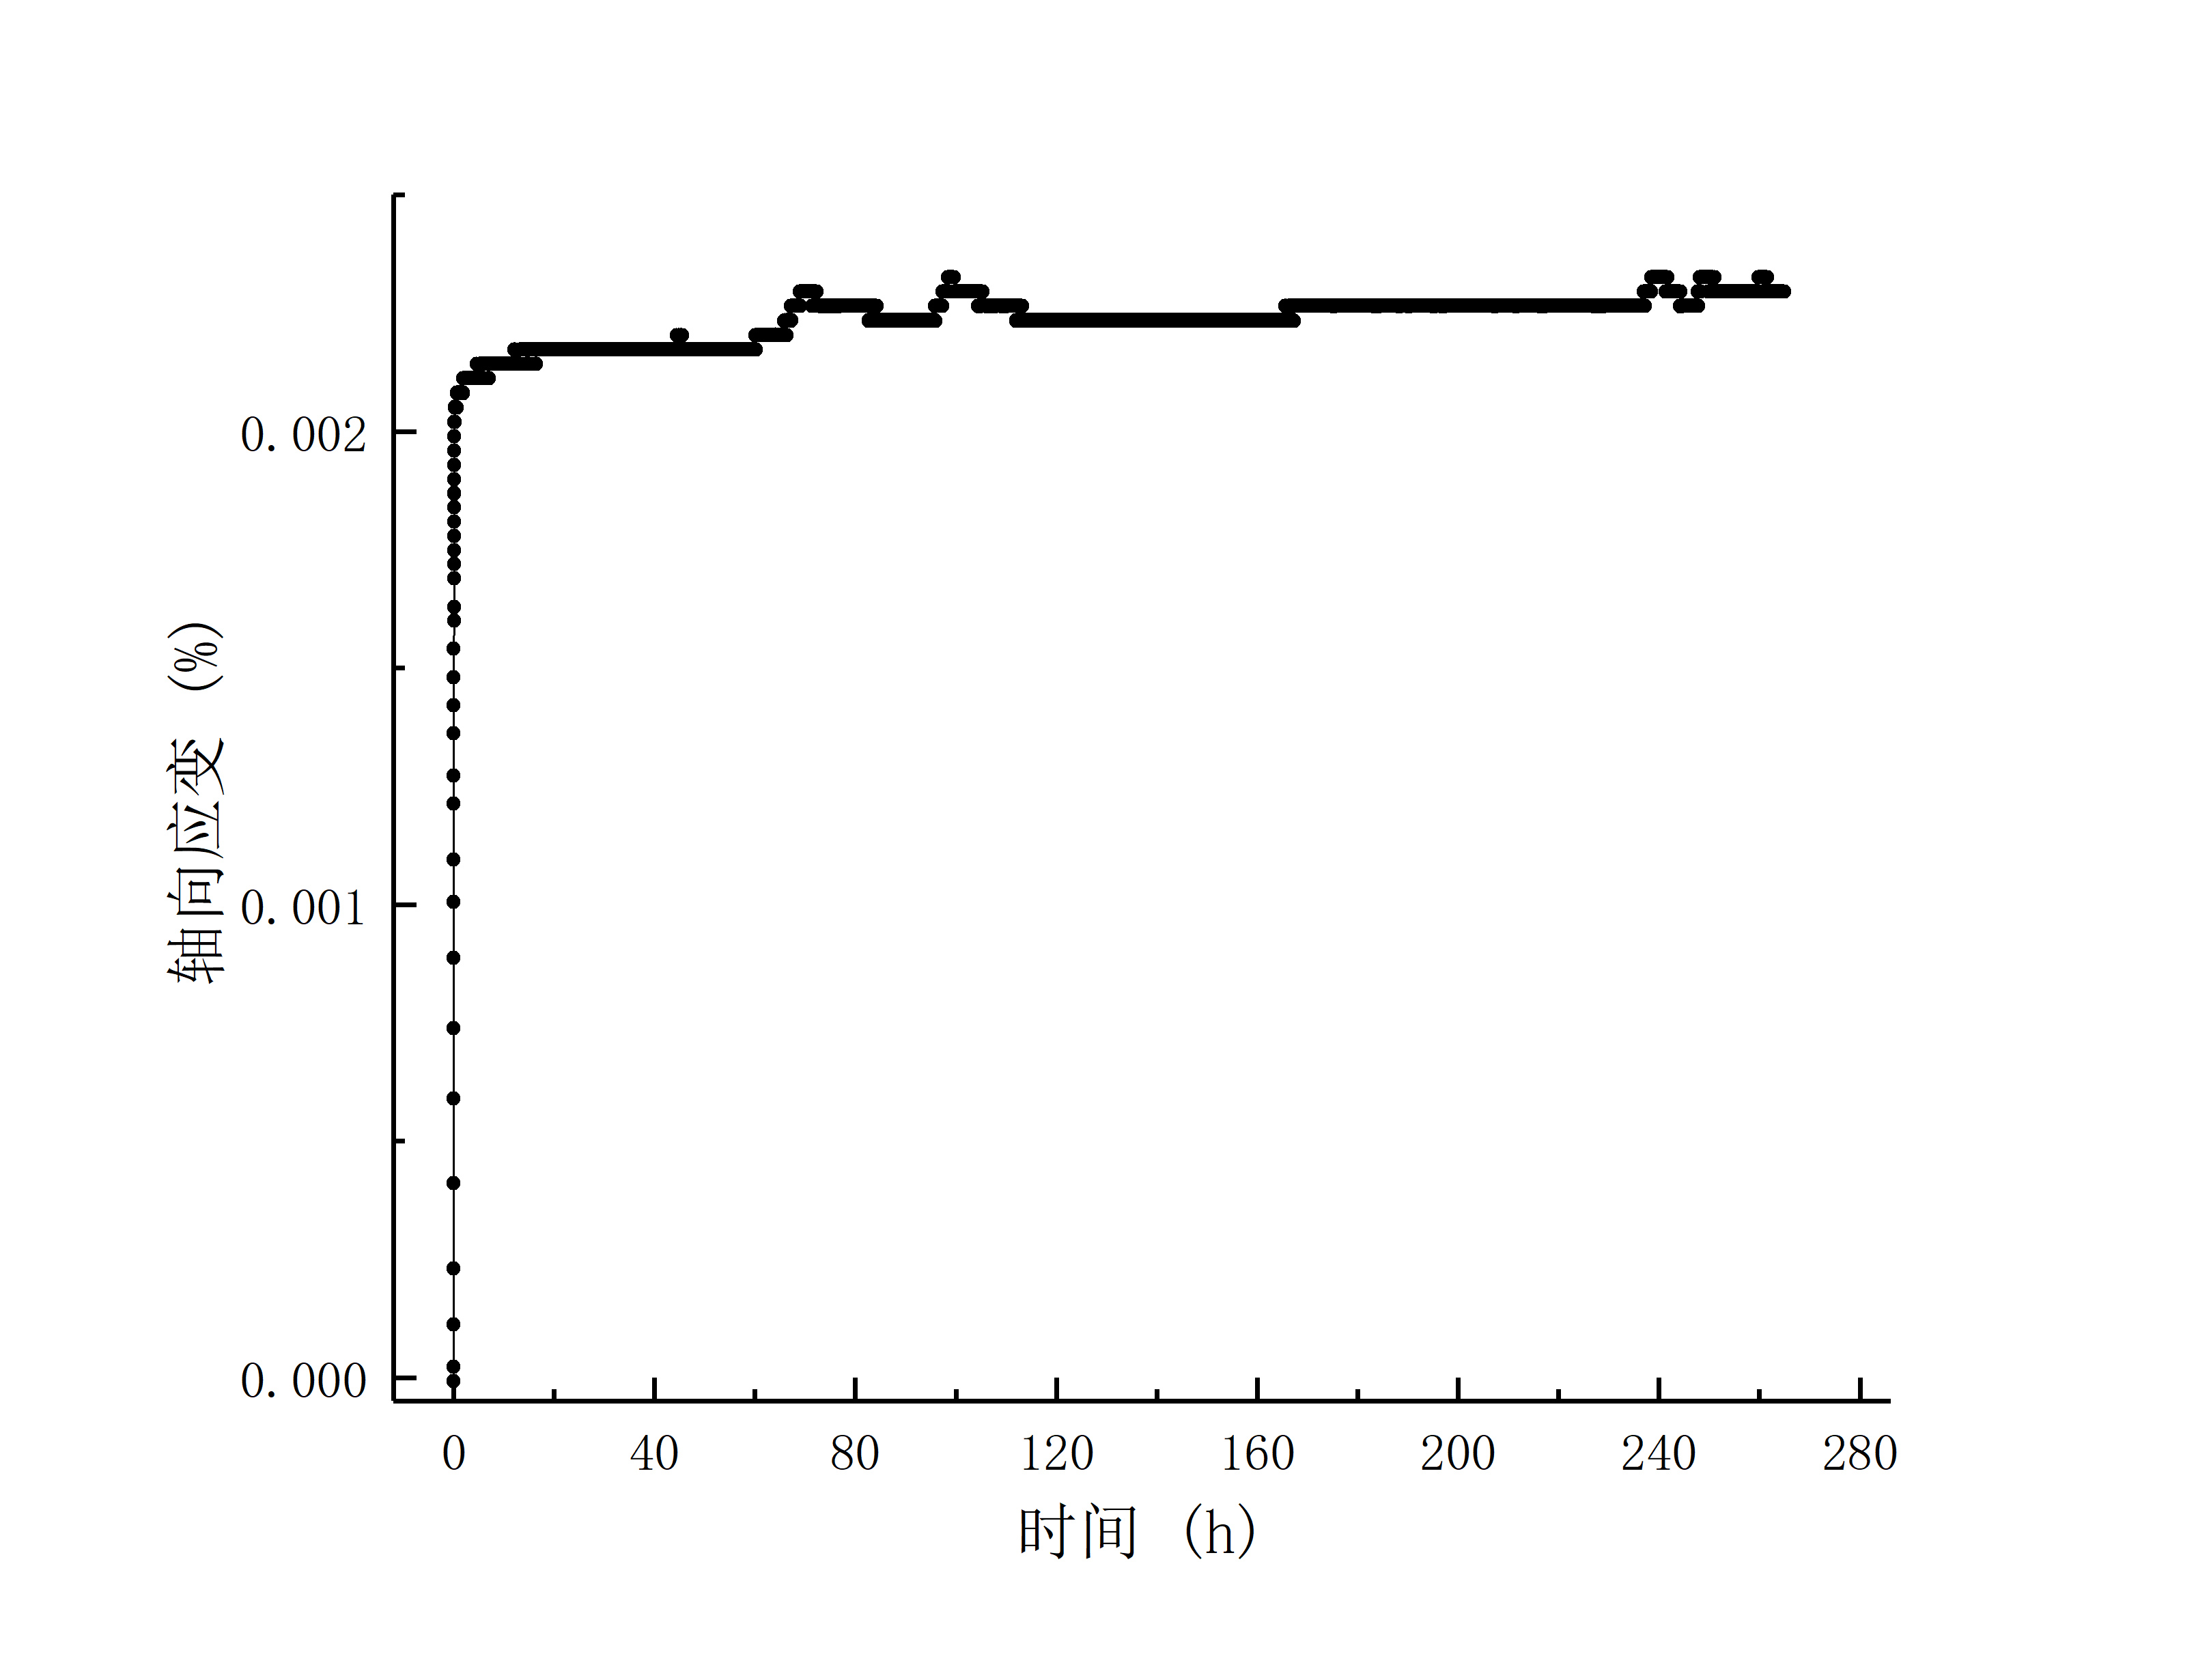
\includegraphics[width=1.1\textwidth]{img/chap2/C-04.png}
        \end{minipage}
    }
    \centering
    \subfigure[C-05]
    {
        \begin{minipage}{7cm}
            \centering
            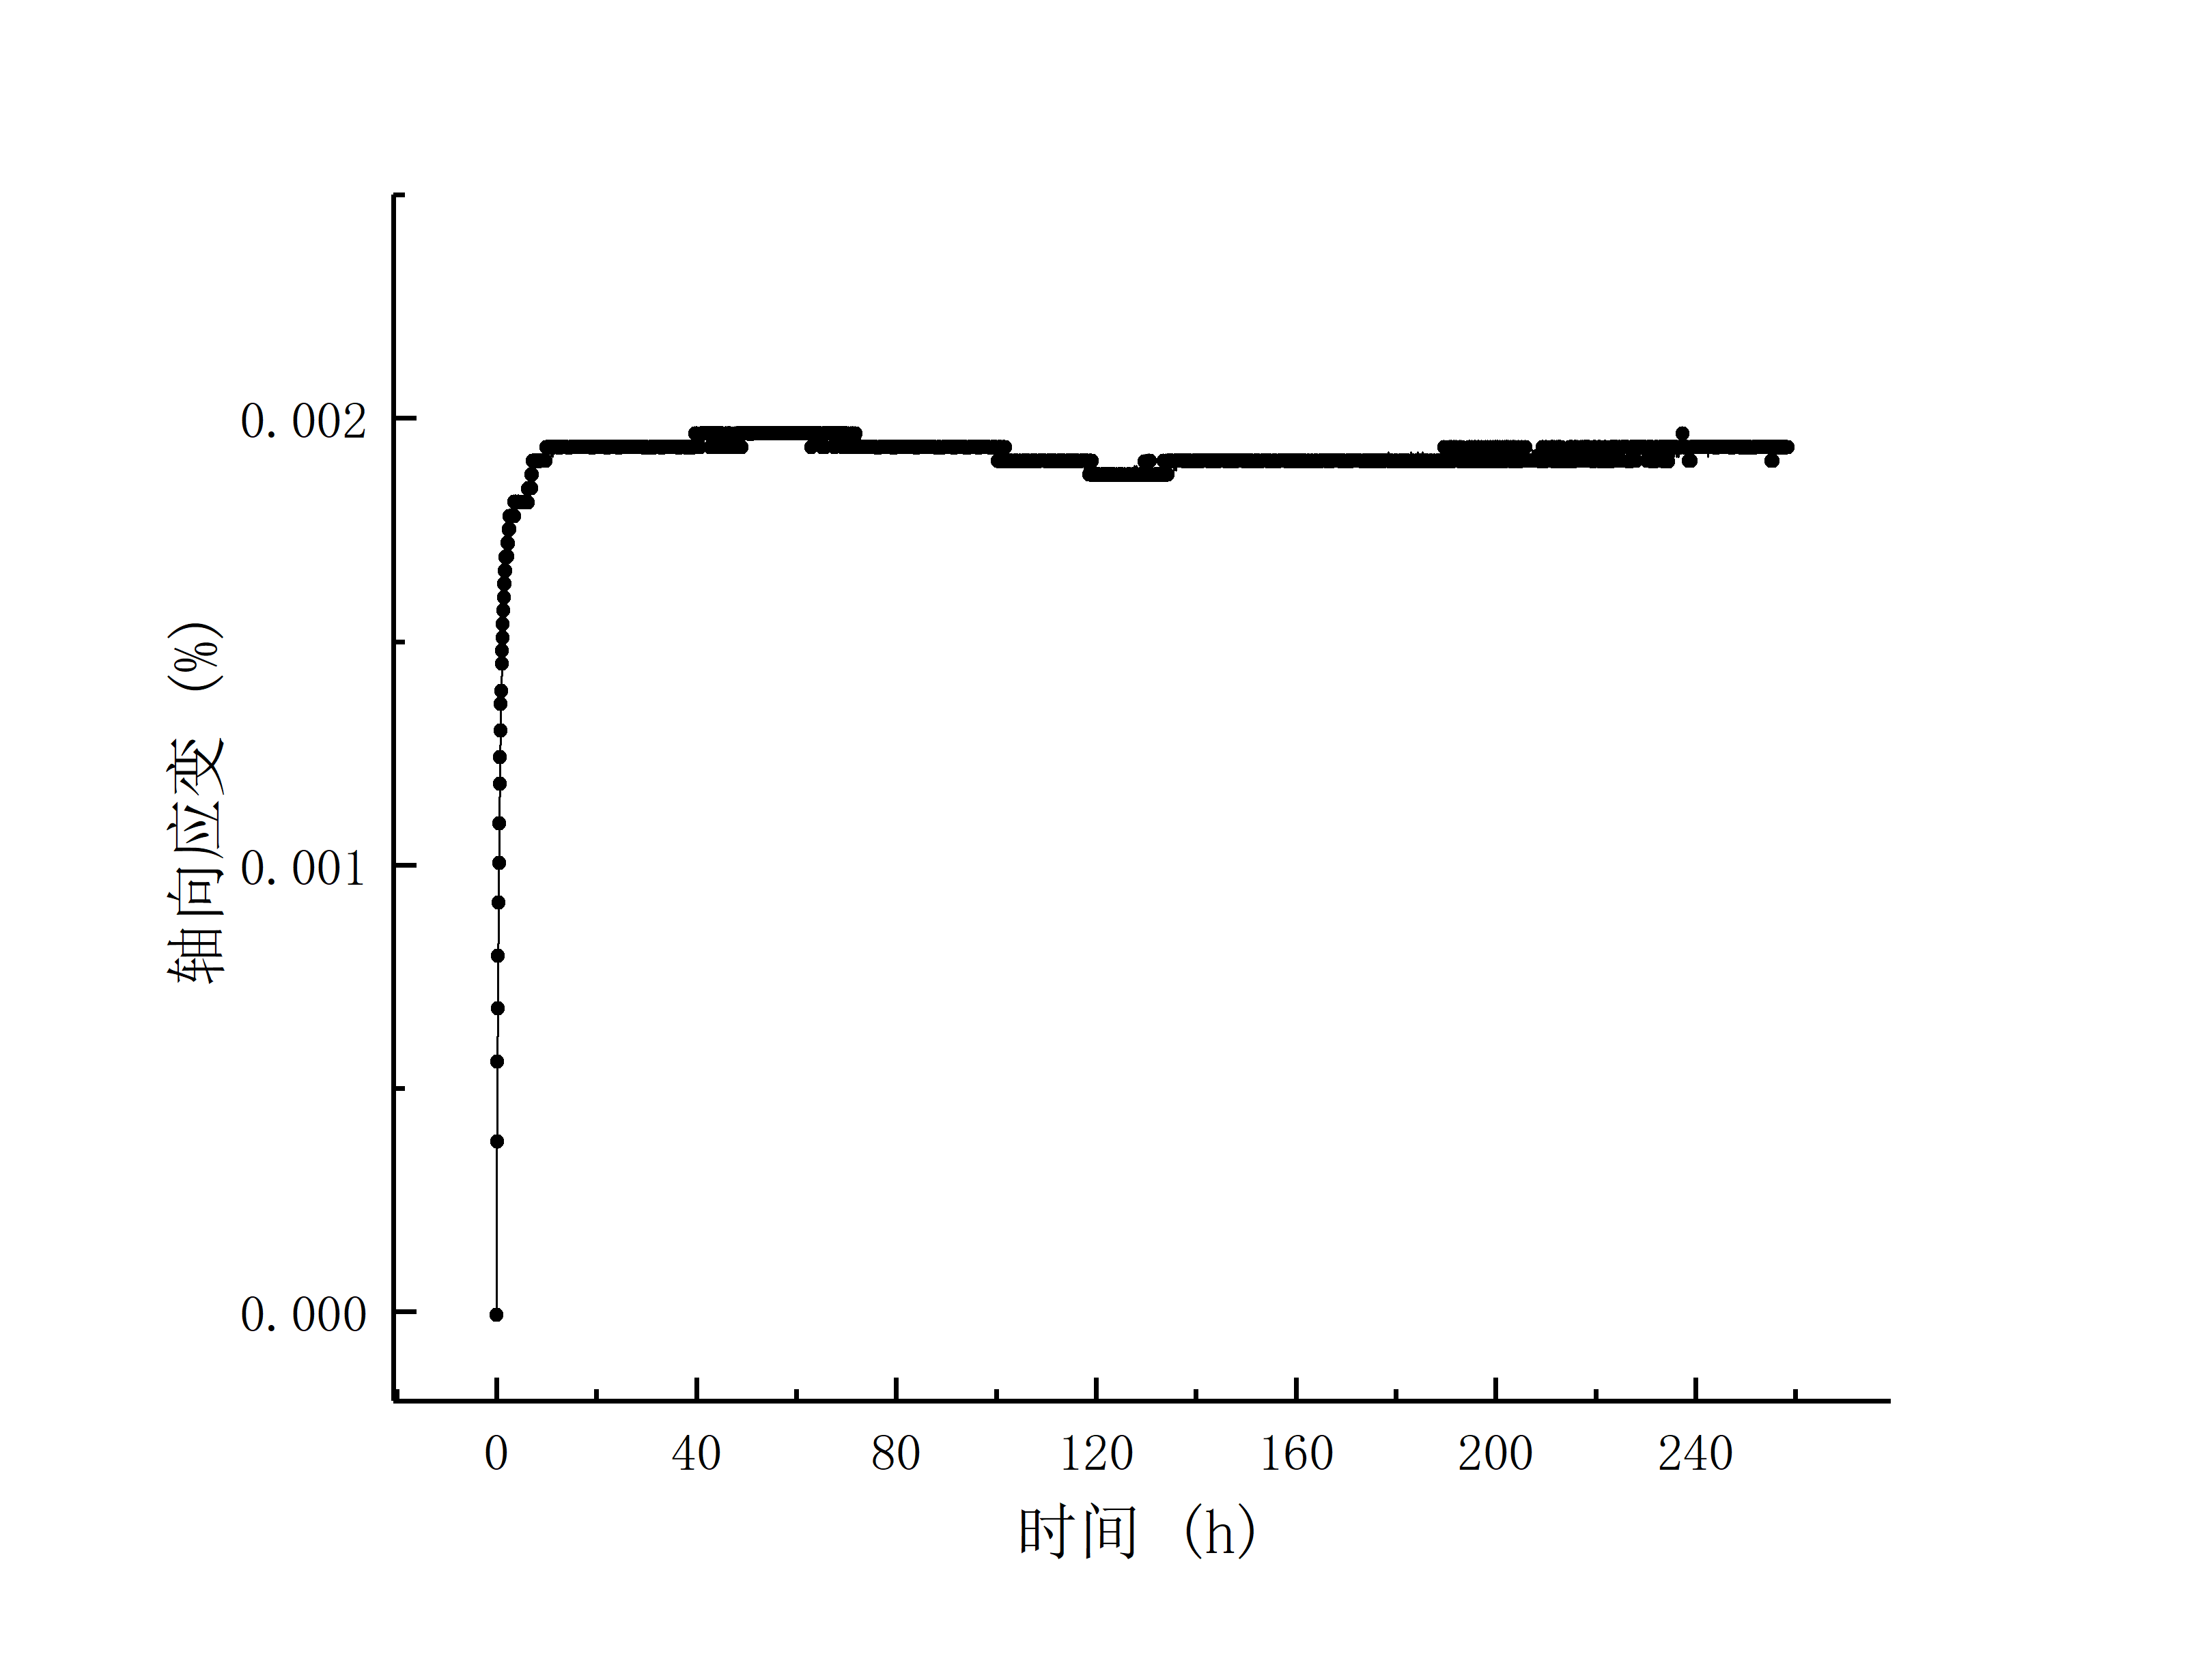
\includegraphics[width=1.1\textwidth]{img/chap2/C-05.png}
        \end{minipage}
    }
    \centering
    \caption{泥岩单轴压缩蠕变试验曲线图}
    \label{fig:2-9}
\end{figure}

\subsection{流变速率分析}
岩石的蠕变速率是描述岩石在恒定应力下变形快慢的物理量,也是研宄岩石蠕变特性的重要指标。分析蠕变试验数据,可以发现,在蠕变微段时间内蠕变速率波动大,这主要是由于岩样内部微观结构蠕变发展的非连续性所导致的。采用张春阳等\cite{张春阳}在文中分析深部斜长角闪岩蠕变速率的方法来计算泥岩蠕变试验分级加载过程中的蠕变速率
,在不影响速率趋势的情况下,选择$\Delta{t_i}$时间内n个蠕变数据,计算第n个和第n-1
个蠕变数据的差值(n>1),以此类推,求得各差值之和,这就是在$\Delta{t_i}$时间内试样的总蠕变量。将算出的第i段时间内的总蠕变量除以第i段的总时间,就可获得第i段时间内的螺变速率$v_i$,计算过程为如下:

\begin{equation}
  \left\{
  \begin{aligned}
 &\Delta{\varepsilon} =\Delta{\varepsilon_1}+\Delta{\varepsilon_2}+\cdots+\Delta{\varepsilon_{n-1}}  \\
 & \Delta{\varepsilon_1}=\varepsilon_2-\varepsilon_1,\Delta{\varepsilon_2}=\varepsilon_3-\varepsilon_2,\Delta{\varepsilon_{n-1}}=\varepsilon_n-\varepsilon_{n-1}\\ 
 & \Delta{\varepsilon}=(\varepsilon_2+\varepsilon_3+\cdots+\varepsilon_n)-(\varepsilon_1+\varepsilon_2+\cdots+\varepsilon_{n-1})=\varepsilon_n-\varepsilon_1  \\
 & {v_i}=\Delta{\varepsilon}/\Delta{t_i}
 \end{aligned}
 \right.
\end{equation}

其中,$\varepsilon_1,\varepsilon_2,\cdots,\varepsilon_n$为各段的轴向应变值;$\Delta{\varepsilon_1},\Delta{\varepsilon_2},\cdots,\Delta{\varepsilon_n}$是各微段轴向应变值之差,$\Delta{\varepsilon}$和$v_i$表示$\Delta{t_i}$时间段内的总应变和平均应变速率,将求得的相邻时间段内的应变速率连成曲线,各试样具体的流变速率如图~\ref{fig:2-10}所示:

\begin{figure}[ht!]
    \centering
    \subfigure[C-01]
    {
        \begin{minipage}{7cm}
            \centering
            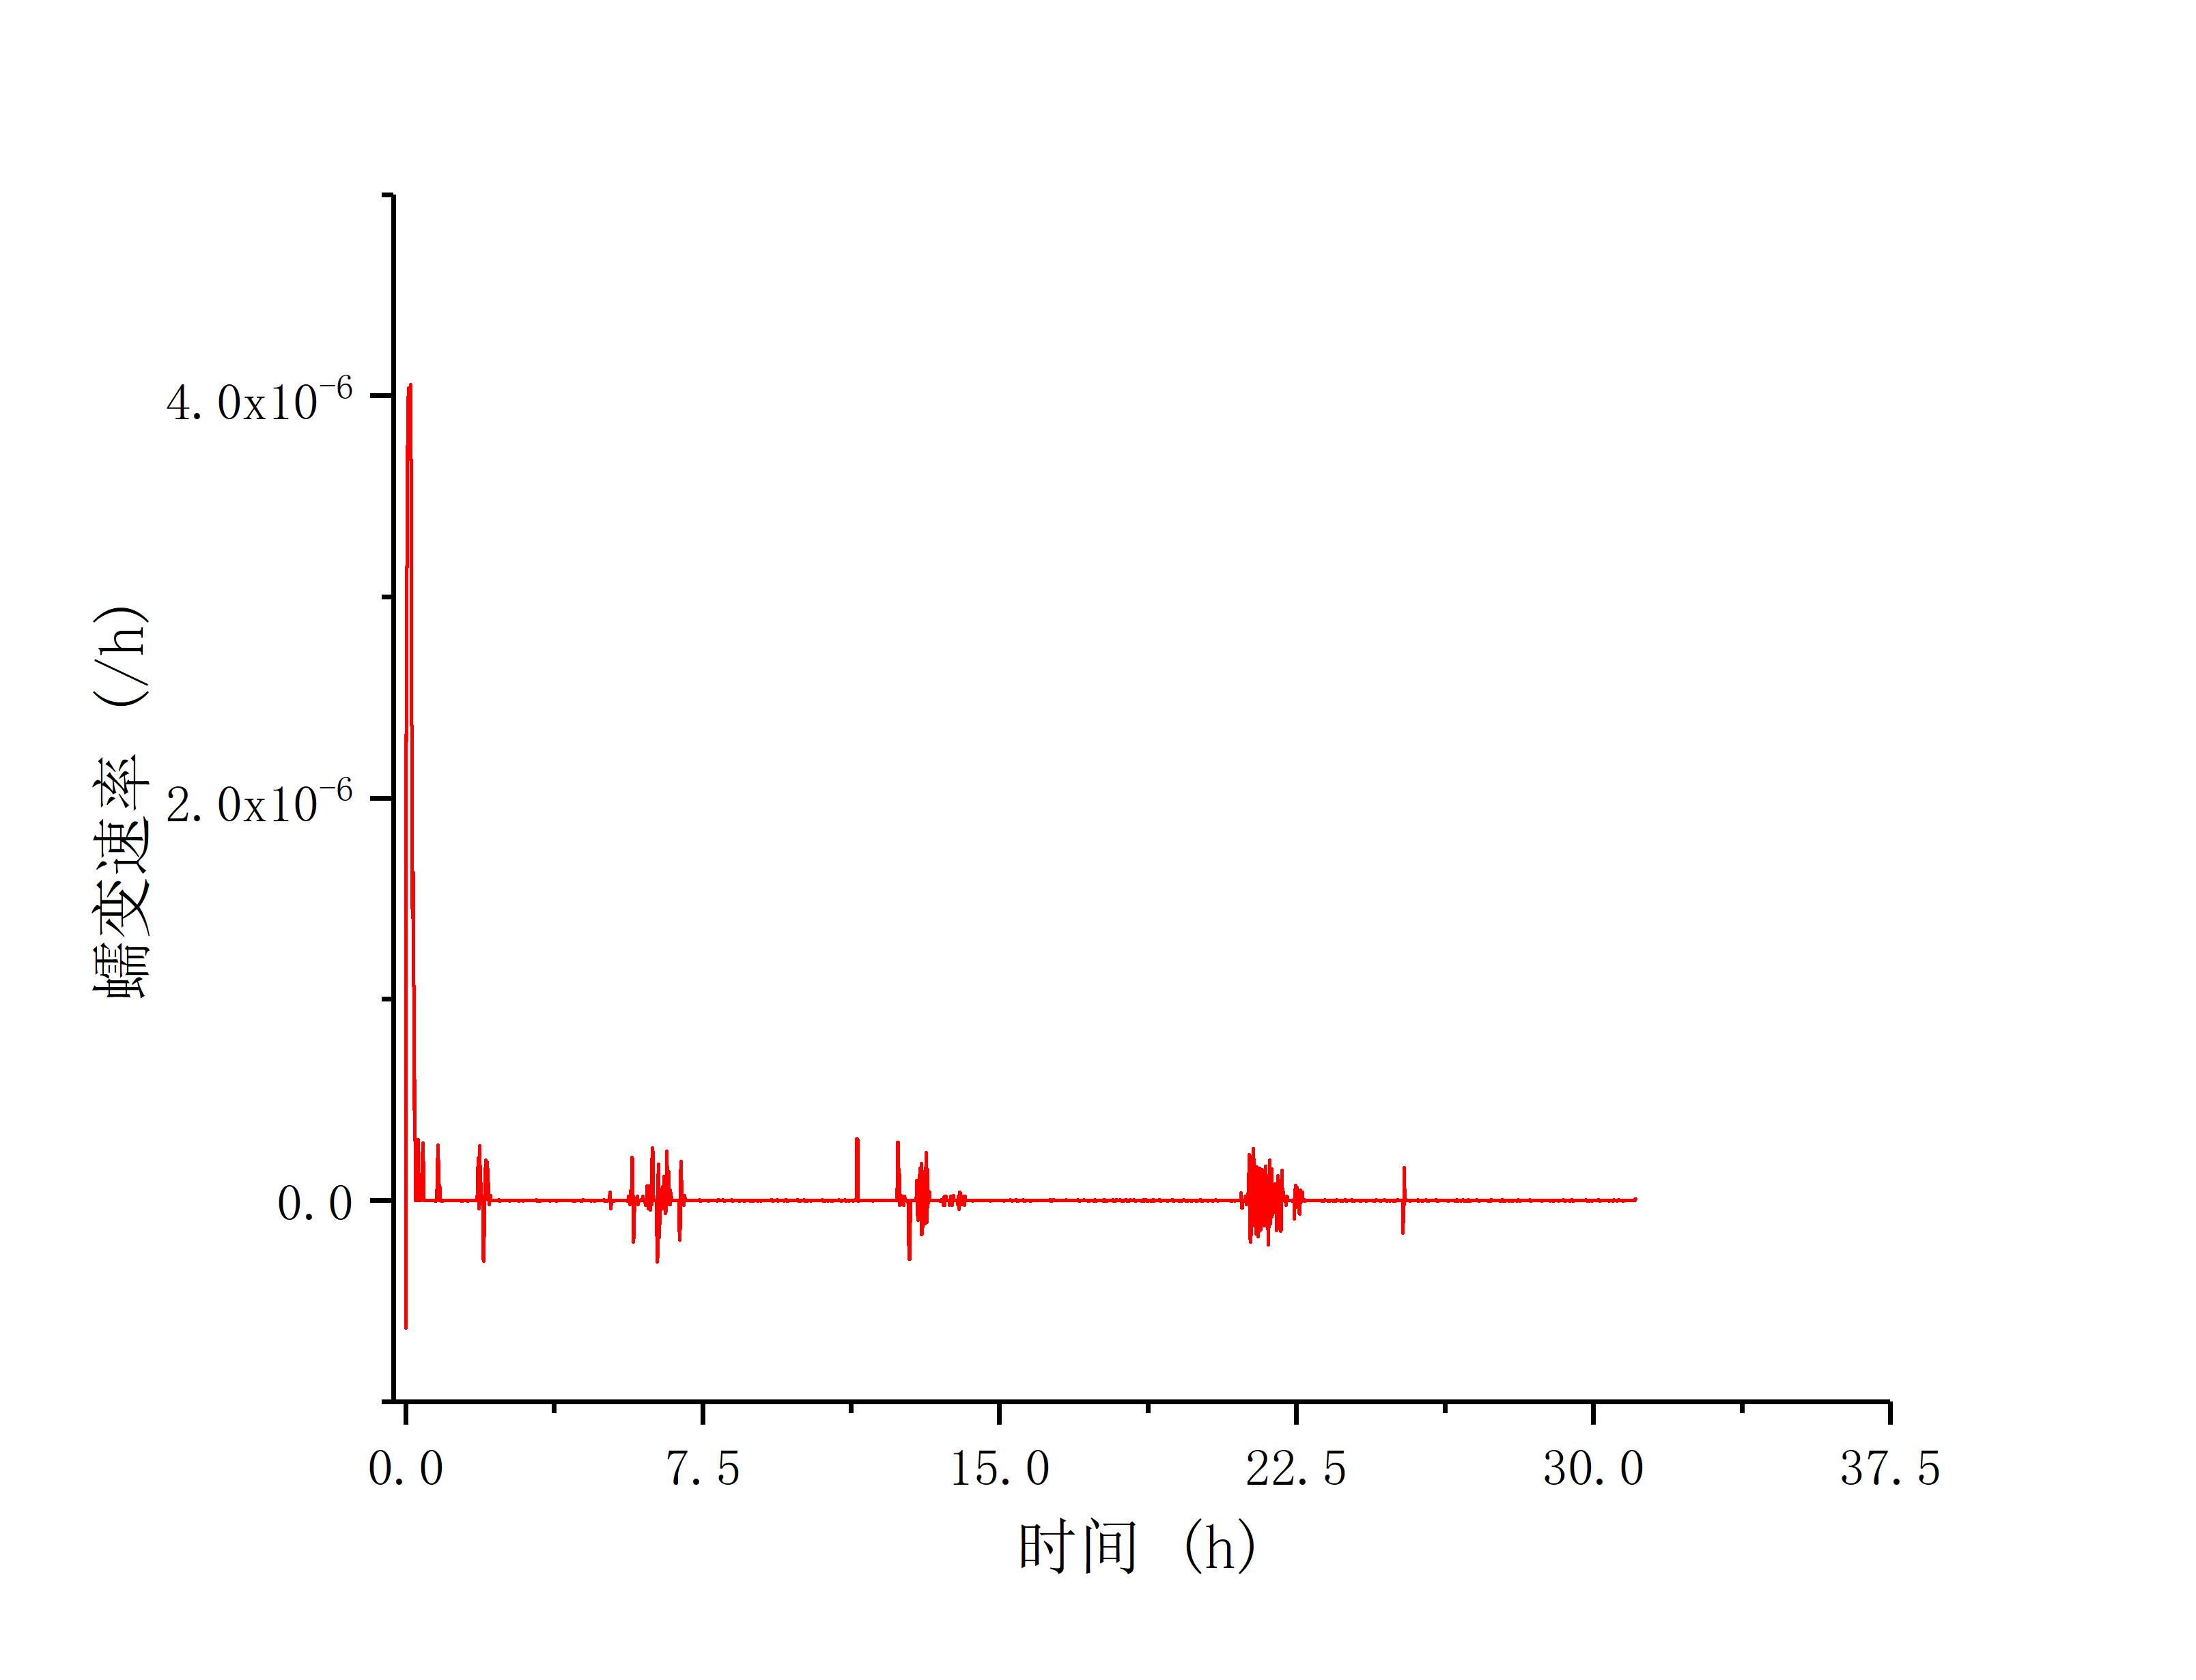
\includegraphics[width=1.1\textwidth]{img/chap2/C-01-v.png}
        \end{minipage}
    }
    \subfigure[C-02]
    {
        \begin{minipage}{7cm}
            \centering
            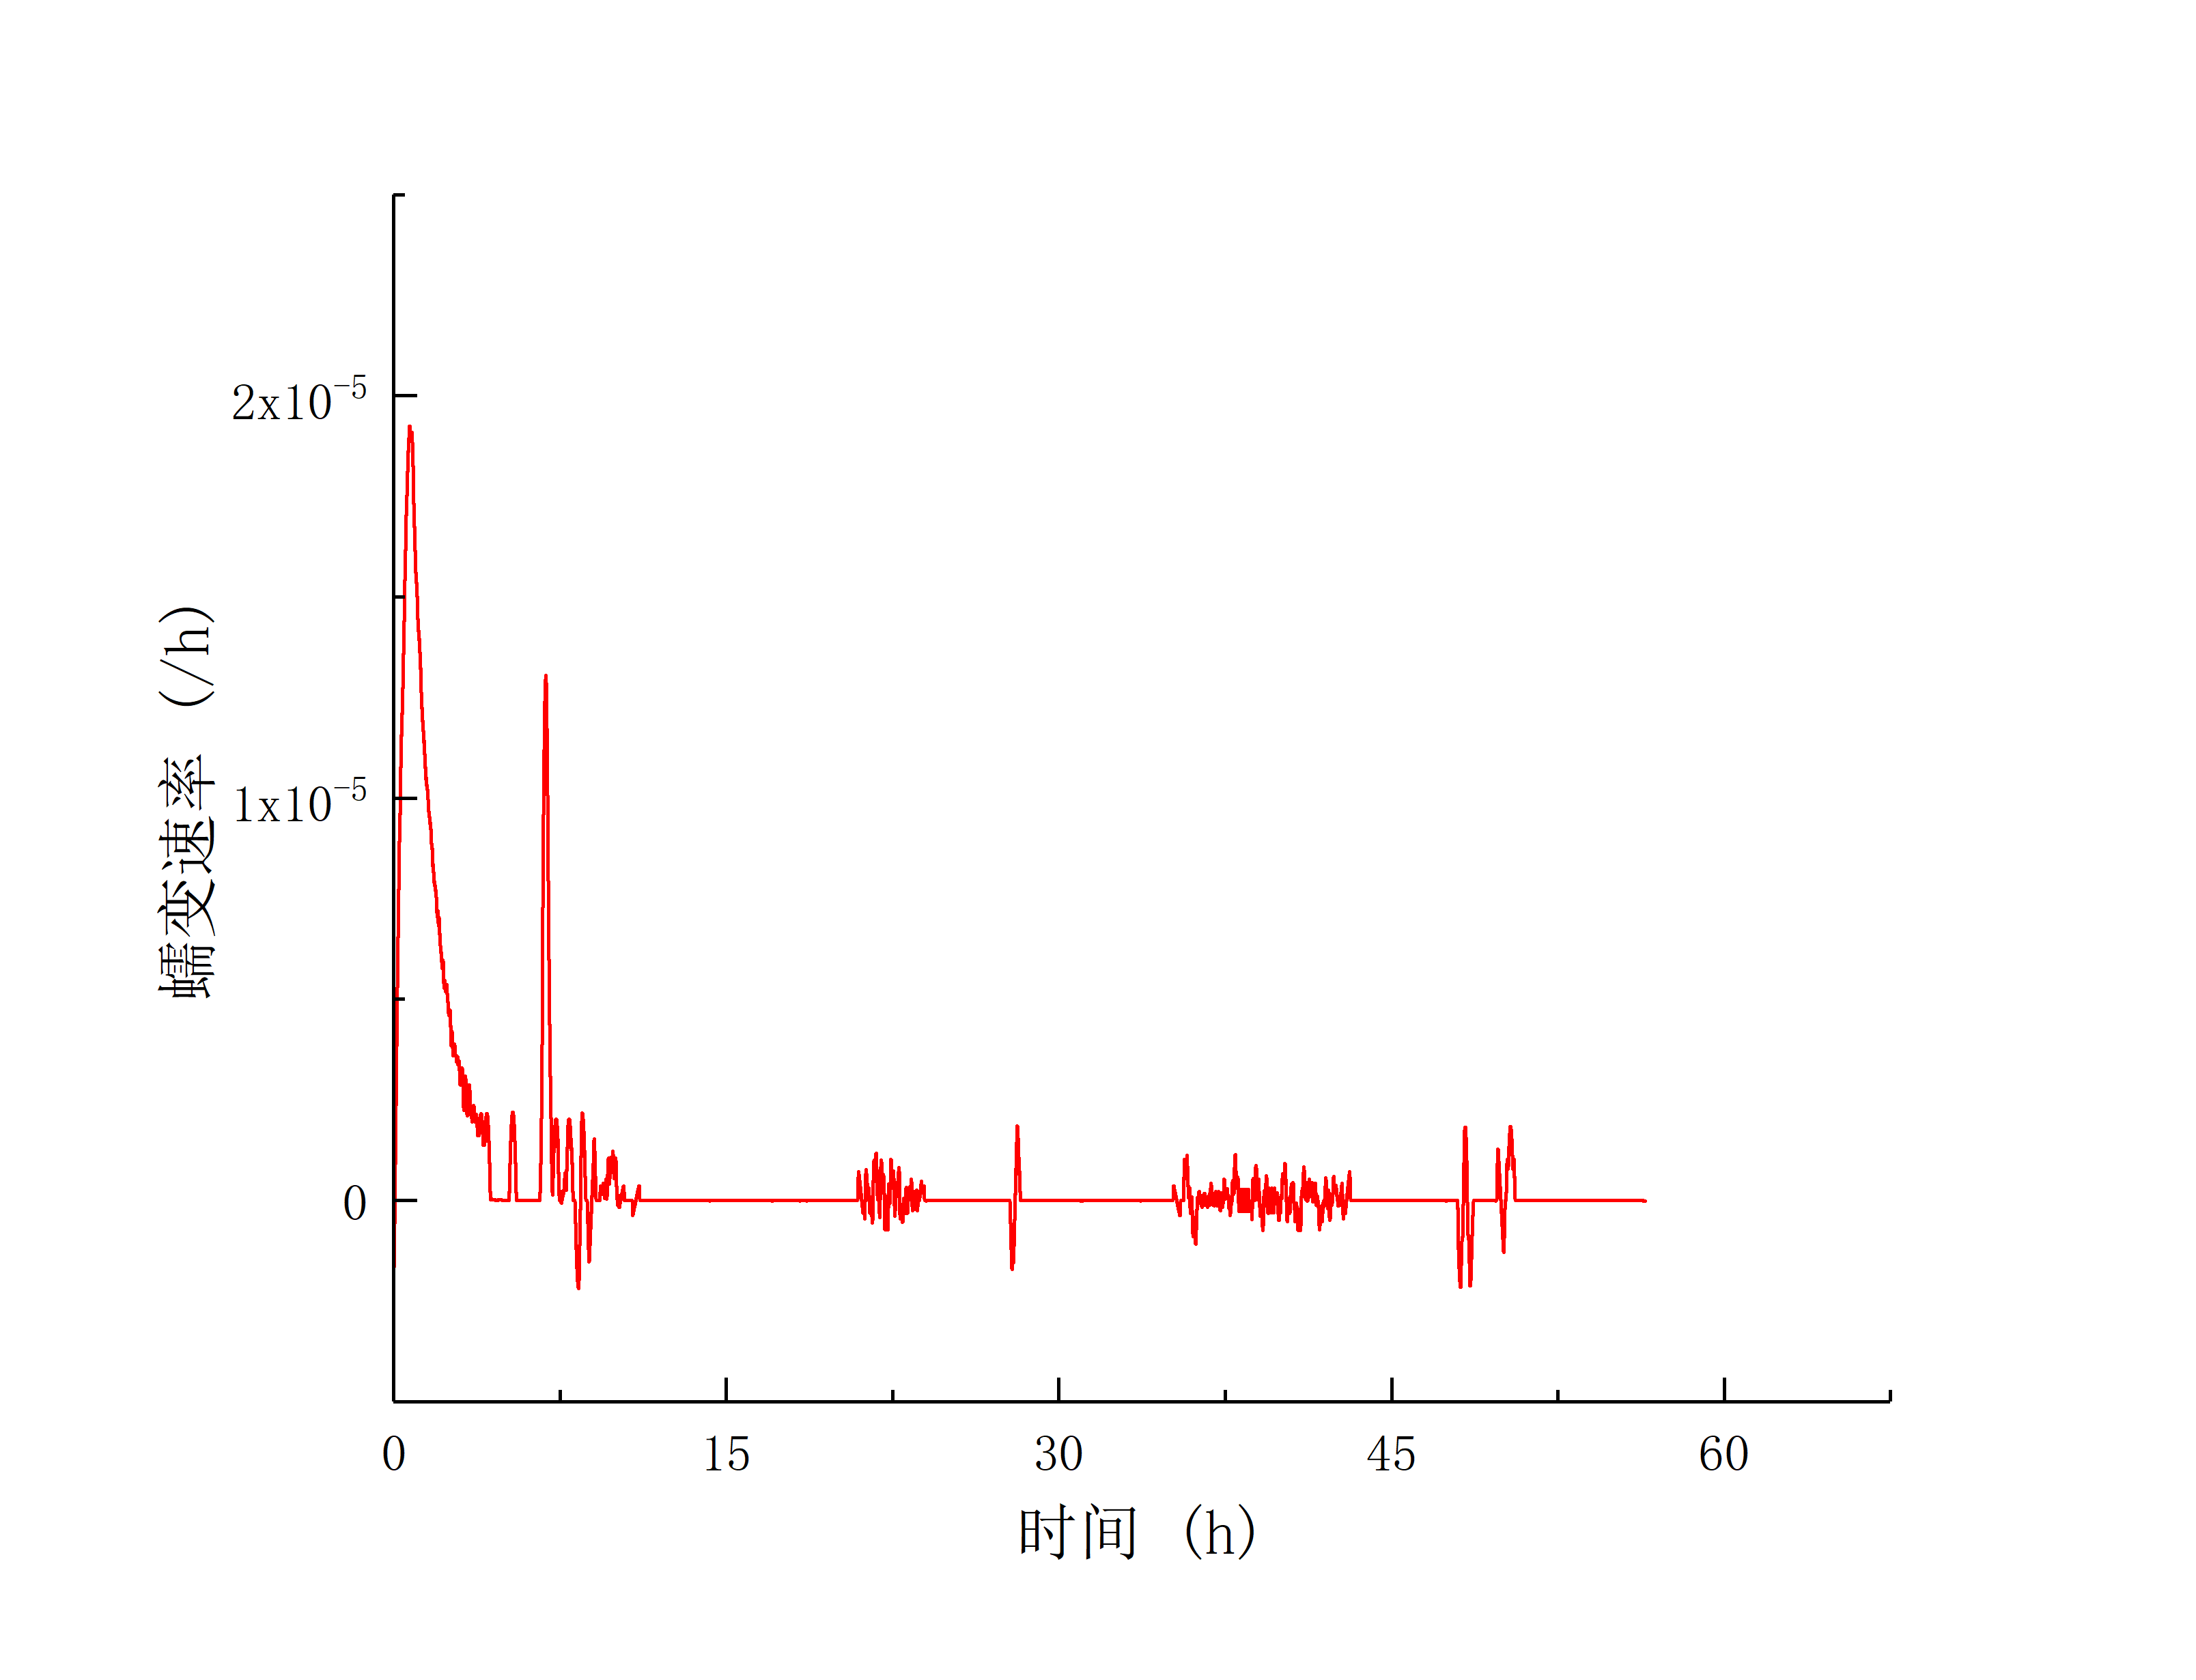
\includegraphics[width=1.1\textwidth]{img/chap2/C-02-v.png}
        \end{minipage}
    }
    \subfigure[C-04]
    {
        \begin{minipage}{7cm}
            \centering
            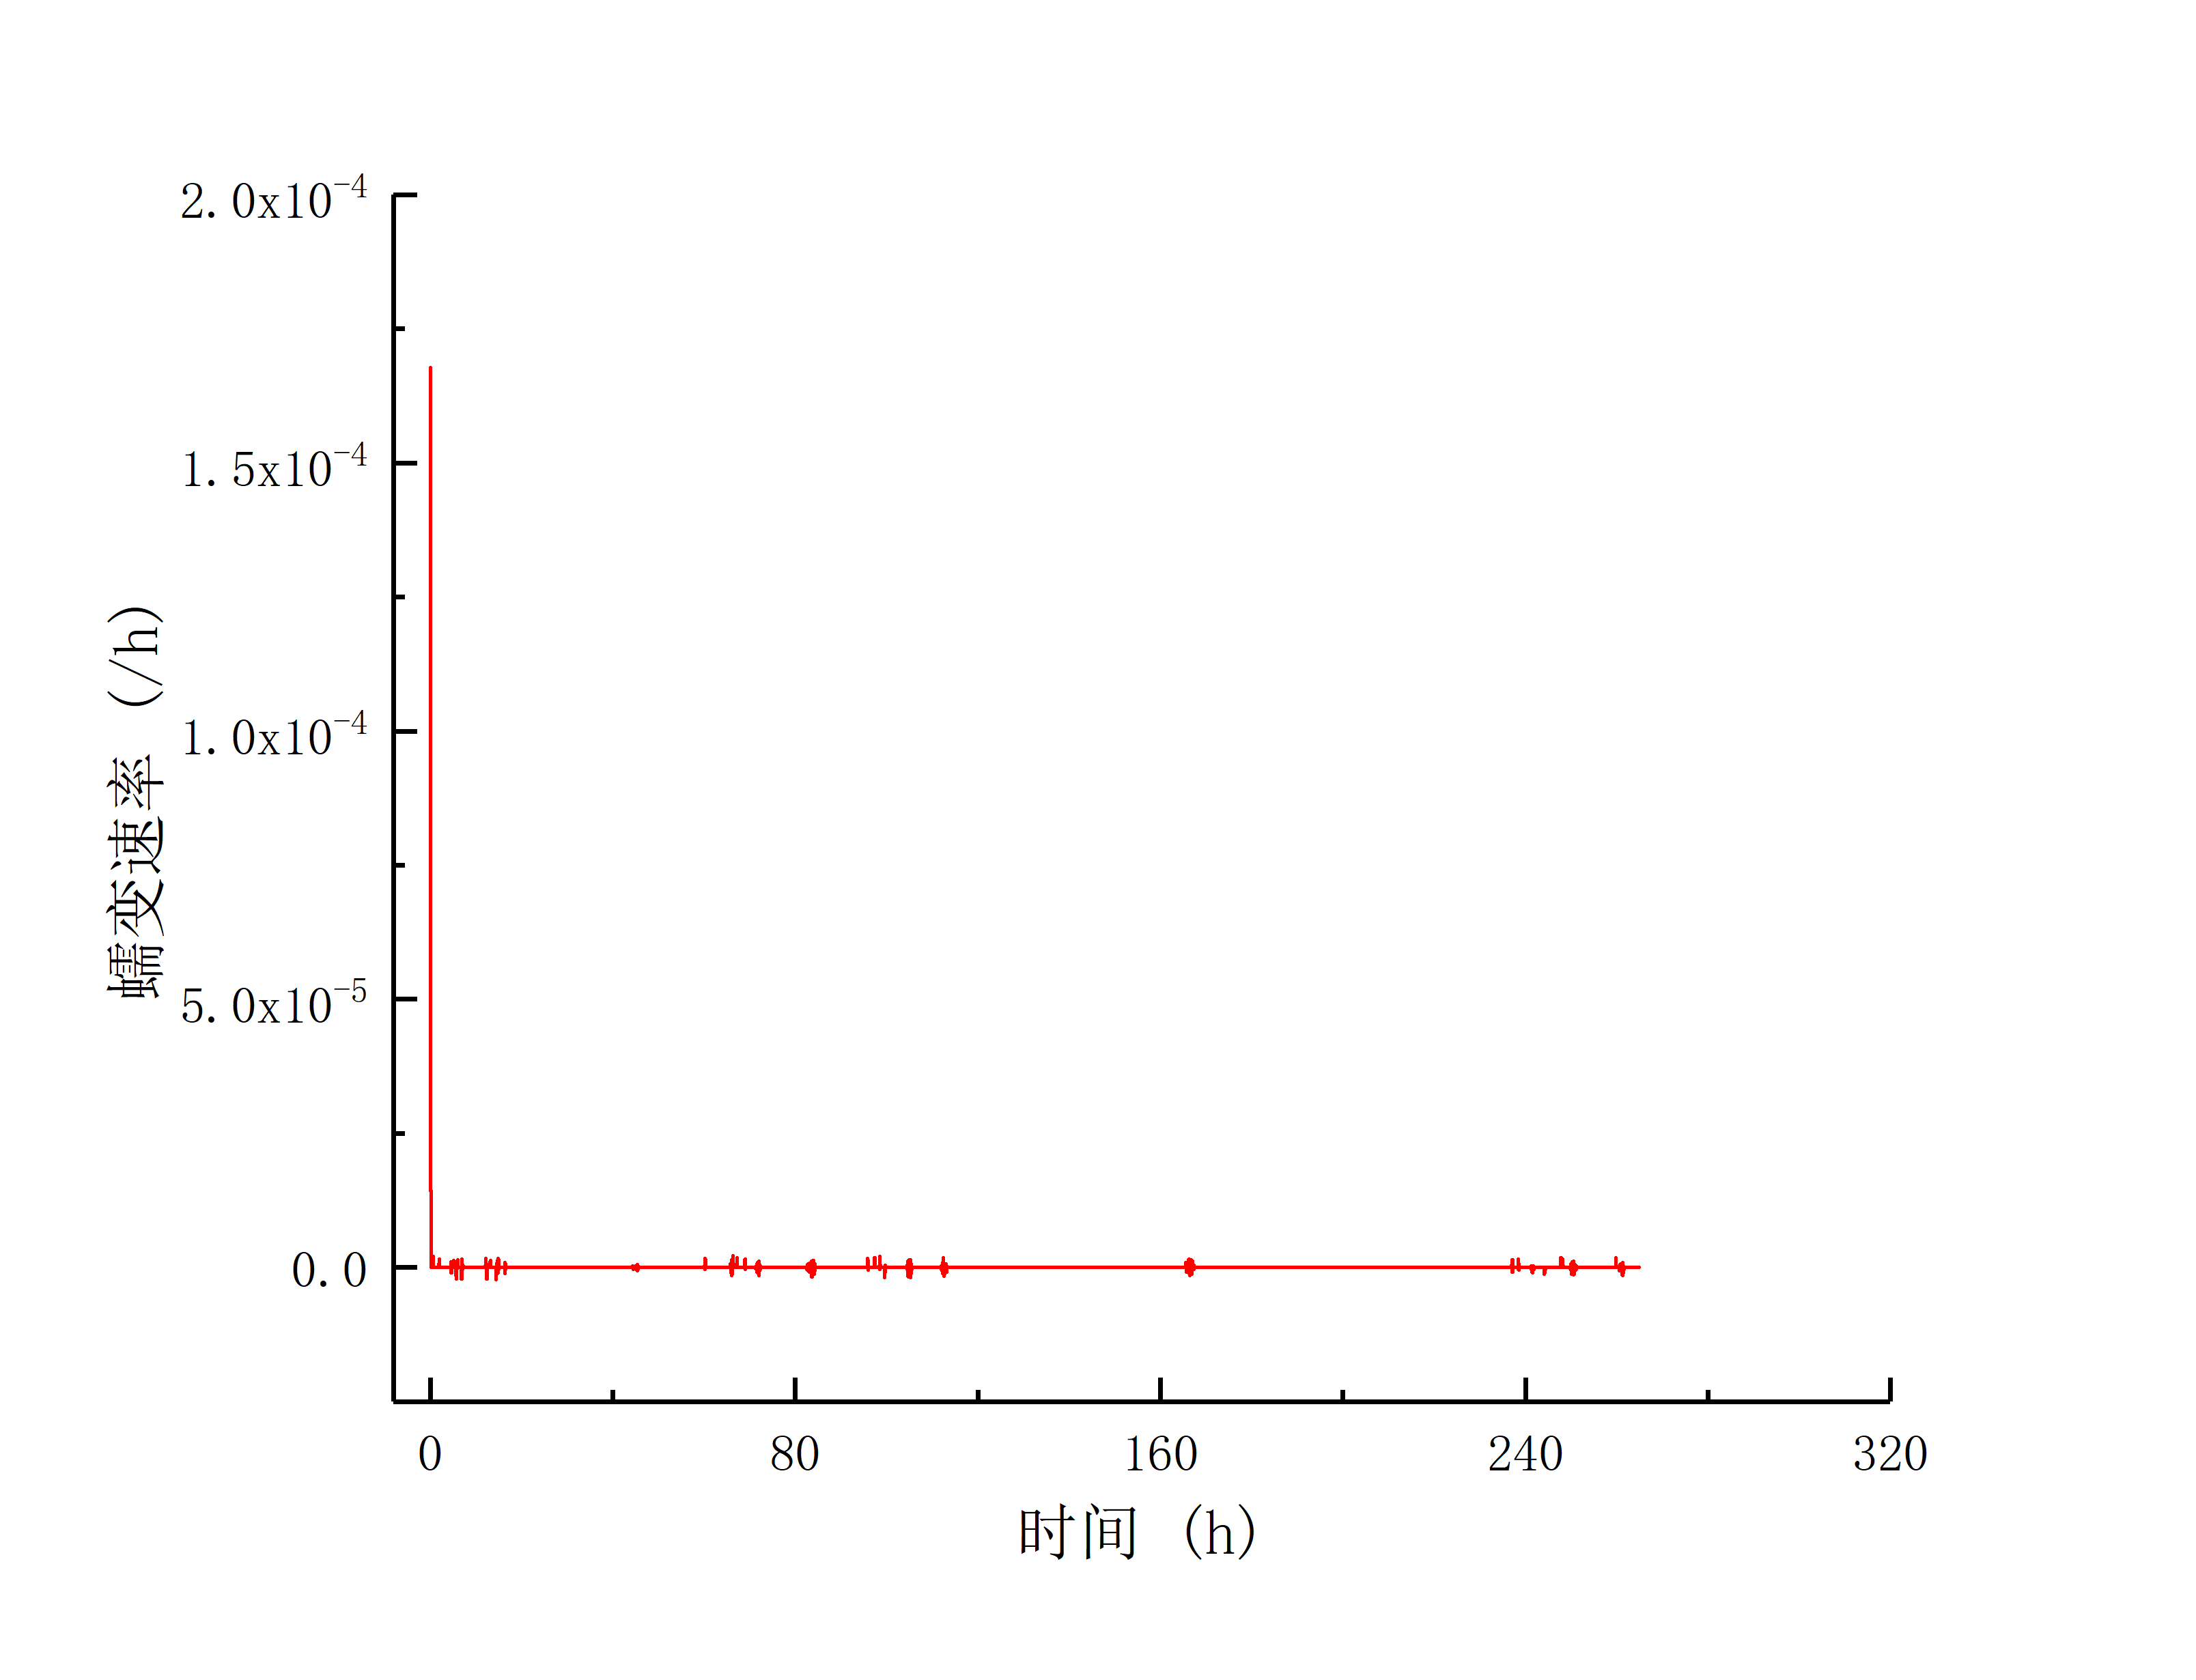
\includegraphics[width=1.1\textwidth]{img/chap2/C-04-v.png}
        \end{minipage}
    }
    \centering
    \subfigure[C-05]
    {
        \begin{minipage}{7cm}
            \centering
            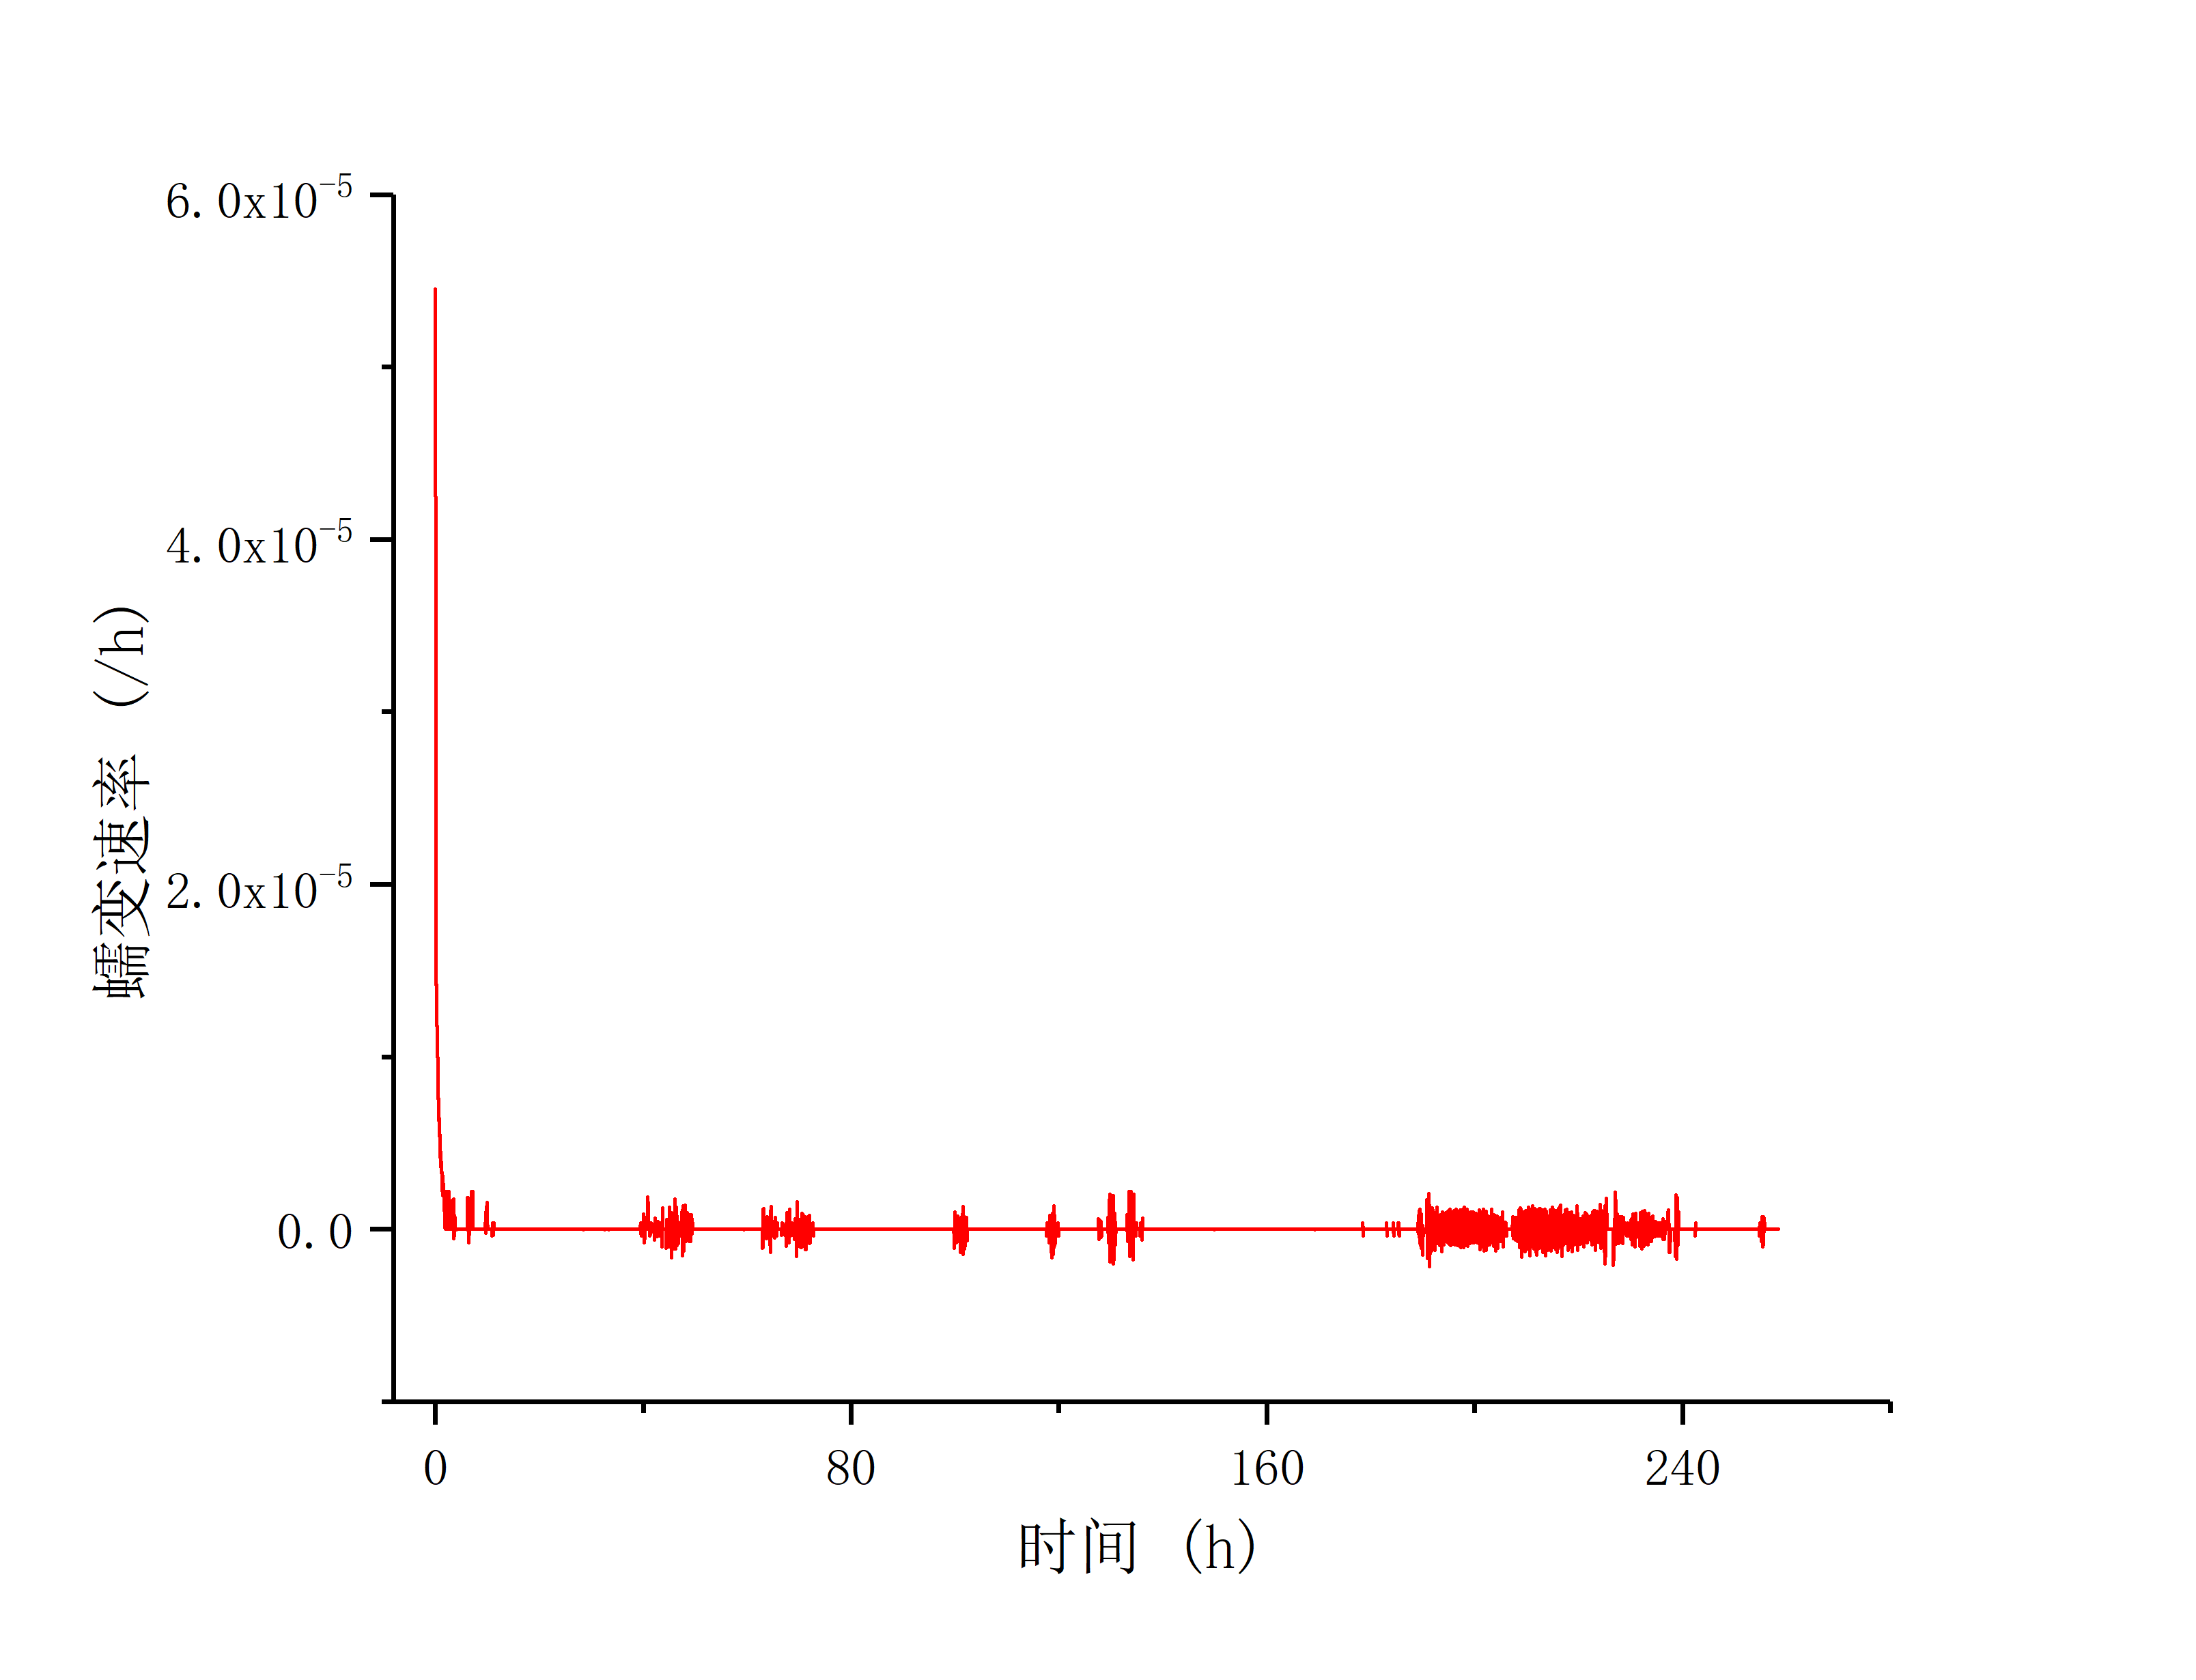
\includegraphics[width=1.1\textwidth]{img/chap2/C-05-v.png}
        \end{minipage}
    }
    \centering
    \caption{泥岩单轴压缩蠕变速率曲线图}
    \label{fig:2-10}
\end{figure}

以下四张图为单轴流变试验中试样流变速率的曲线图,C-03因为试样很快破坏,因此不进行流变速率分析。
在流变试验中,施加一定的应力值,在试样进入流变阶段后,首先会进入流变速率不断减小的衰减蠕变阶段,
从图中我们可以看出,在瞬时应变发生到流变变形开始前的这个短暂的时间内,随着瞬时应变的增大,流变速率会快速增长至最大值。之后,在初始蠕变阶段,流变速率会随着时间的增长逐渐减小的,并且在初始阶段都衰减的十分迅速,不断发展趋于与横轴平行的近似直线,当流变速率衰减到某一定值时,流变进入稳定发展阶段,
若施加的初始应力较小,蠕变速率会一直减小到无限接近于零,如果施加的应力较大,试样的蠕变速率则会减小到某一非零的常数并保持不变,此对应的流变速率为稳态流变速率,试样的蠕变变形随着时间稳定增加。

由图我们可以看出,岩石在蠕变过程中的大多数时间都是处于稳定蠕变阶段,在这个过程中,岩石的变形逐步积累,内部裂隙不断发展,直至试样破坏。总体来说,相同岩石的初始蠕变速率及稳态蠕变速率随着应力水平的增大而增大,不过在单轴蠕变试验采取的是分别加载的方法,所以试样之间存在差异,导致像分级加载一样准确反应一个试样在不同加载等级下的流变过程与变化规律。当然,由于局部非均匀破裂的影响,泥岩试样在一定应力水平条件下的稳态流变速率会有一定的波动。




\section{泥岩三轴流变试验}
三轴流变试验则是为了研究围压的变化对岩石流变过程应力-应变的影响。选取了三个试样分别编号,测量其具体物理参数,考虑到蠕变试验的时间较长,且制备的试样在进行蠕变试验前还需进行常规三轴压缩试验,试样的数量有限,因此本次三轴流变试验均采用分级加载的方法研究岩石流变特性。泥岩三轴流变试验安排如下表~\ref{tab:泥岩三轴蠕变试验工况表}所示:

\begin{table}[ht!]\small
    \centering
    \begin{threeparttable}
    \begin{tabular}{p{3cm}<{\centering} p{3cm}<{\centering} p{3cm}<{\centering} p{3cm}<{\centering}}
        \toprule
        试样编号  & 围压(MPa)  &  加载等级   &  加载时间(h)\\
        \midrule
                    &    &   0.7$\sigma_\mathrm{F}$   &  24   \\ 
                    &    &   0.7$5\sigma_\mathrm{F}$  &  48   \\ 
        D-01       &  5 &   0.8$\sigma_\mathrm{F}$   &  48  \\
                    &    &   0.85$\sigma_\mathrm{F}$  &  24  \\
                    &    &   0.9$\sigma_\mathrm{F}$  &  24  \\
                    &    &   0.95$\sigma_\mathrm{F}$  &  压至破坏  \\ 
        \midrule
                    &    &   0.7$\sigma_\mathrm{F}$   &  24   \\ 
                    &    &   0.75$\sigma_\mathrm{F}$  &  48   \\ 
        D-02        &  10 &   0.8$\sigma_\mathrm{F}$   &  48  \\
                    &    &   0.85$\sigma_\mathrm{F}$  &  24  \\
                    &    &   0.9$\sigma_\mathrm{F}$  &  24  \\
                    &    &   0.95$\sigma_\mathrm{F}$  &  压至破坏  \\
        \midrule
                    &    &   0.7$\sigma_\mathrm{F}$   &  24   \\ 
                    &    &   0.75$\sigma_\mathrm{F}$  &  48   \\ 
        D-03        &  10 &   0.8$\sigma_\mathrm{F}$   &  48  \\
                    &    &   0.85$\sigma_\mathrm{F}$  &  24  \\
                    &    &   0.9$\sigma_\mathrm{F}$  &  24  \\
                    &    &   0.95$\sigma_\mathrm{F}$  &  压至破坏  \\
        \bottomrule
    \end{tabular}
     \begin{tablenotes}    
        \footnotesize               
        \item 注:$\sigma_F$为三轴压缩试验测得的岩石峰值强度
     \end{tablenotes}            
    \end{threeparttable}       
    \caption{泥岩三轴蠕变试验工况表}
    \label{tab:泥岩三轴蠕变试验工况表}
\end{table}

在三轴流变试验中,我们采用分级加载的方式。在流变实验结束后,我们对收集到的时间、应力、应变数据进行处理,绘制得到单个试样在不同应力等级下的阶梯状时间-应变曲线如图\ref{fig:2-11}所示。各试样在每一级应力加载下均出现流变速率随时间减小的衰减蠕变阶段和流变速率近似不变的稳态蠕变阶段,随着加载应力等级的提高,流变变形量总体呈增加的趋势。


\begin{figure}[ht!]
    \centering
    \subfigure[D-01]
    {
        \begin{minipage}{7cm}
            \centering
            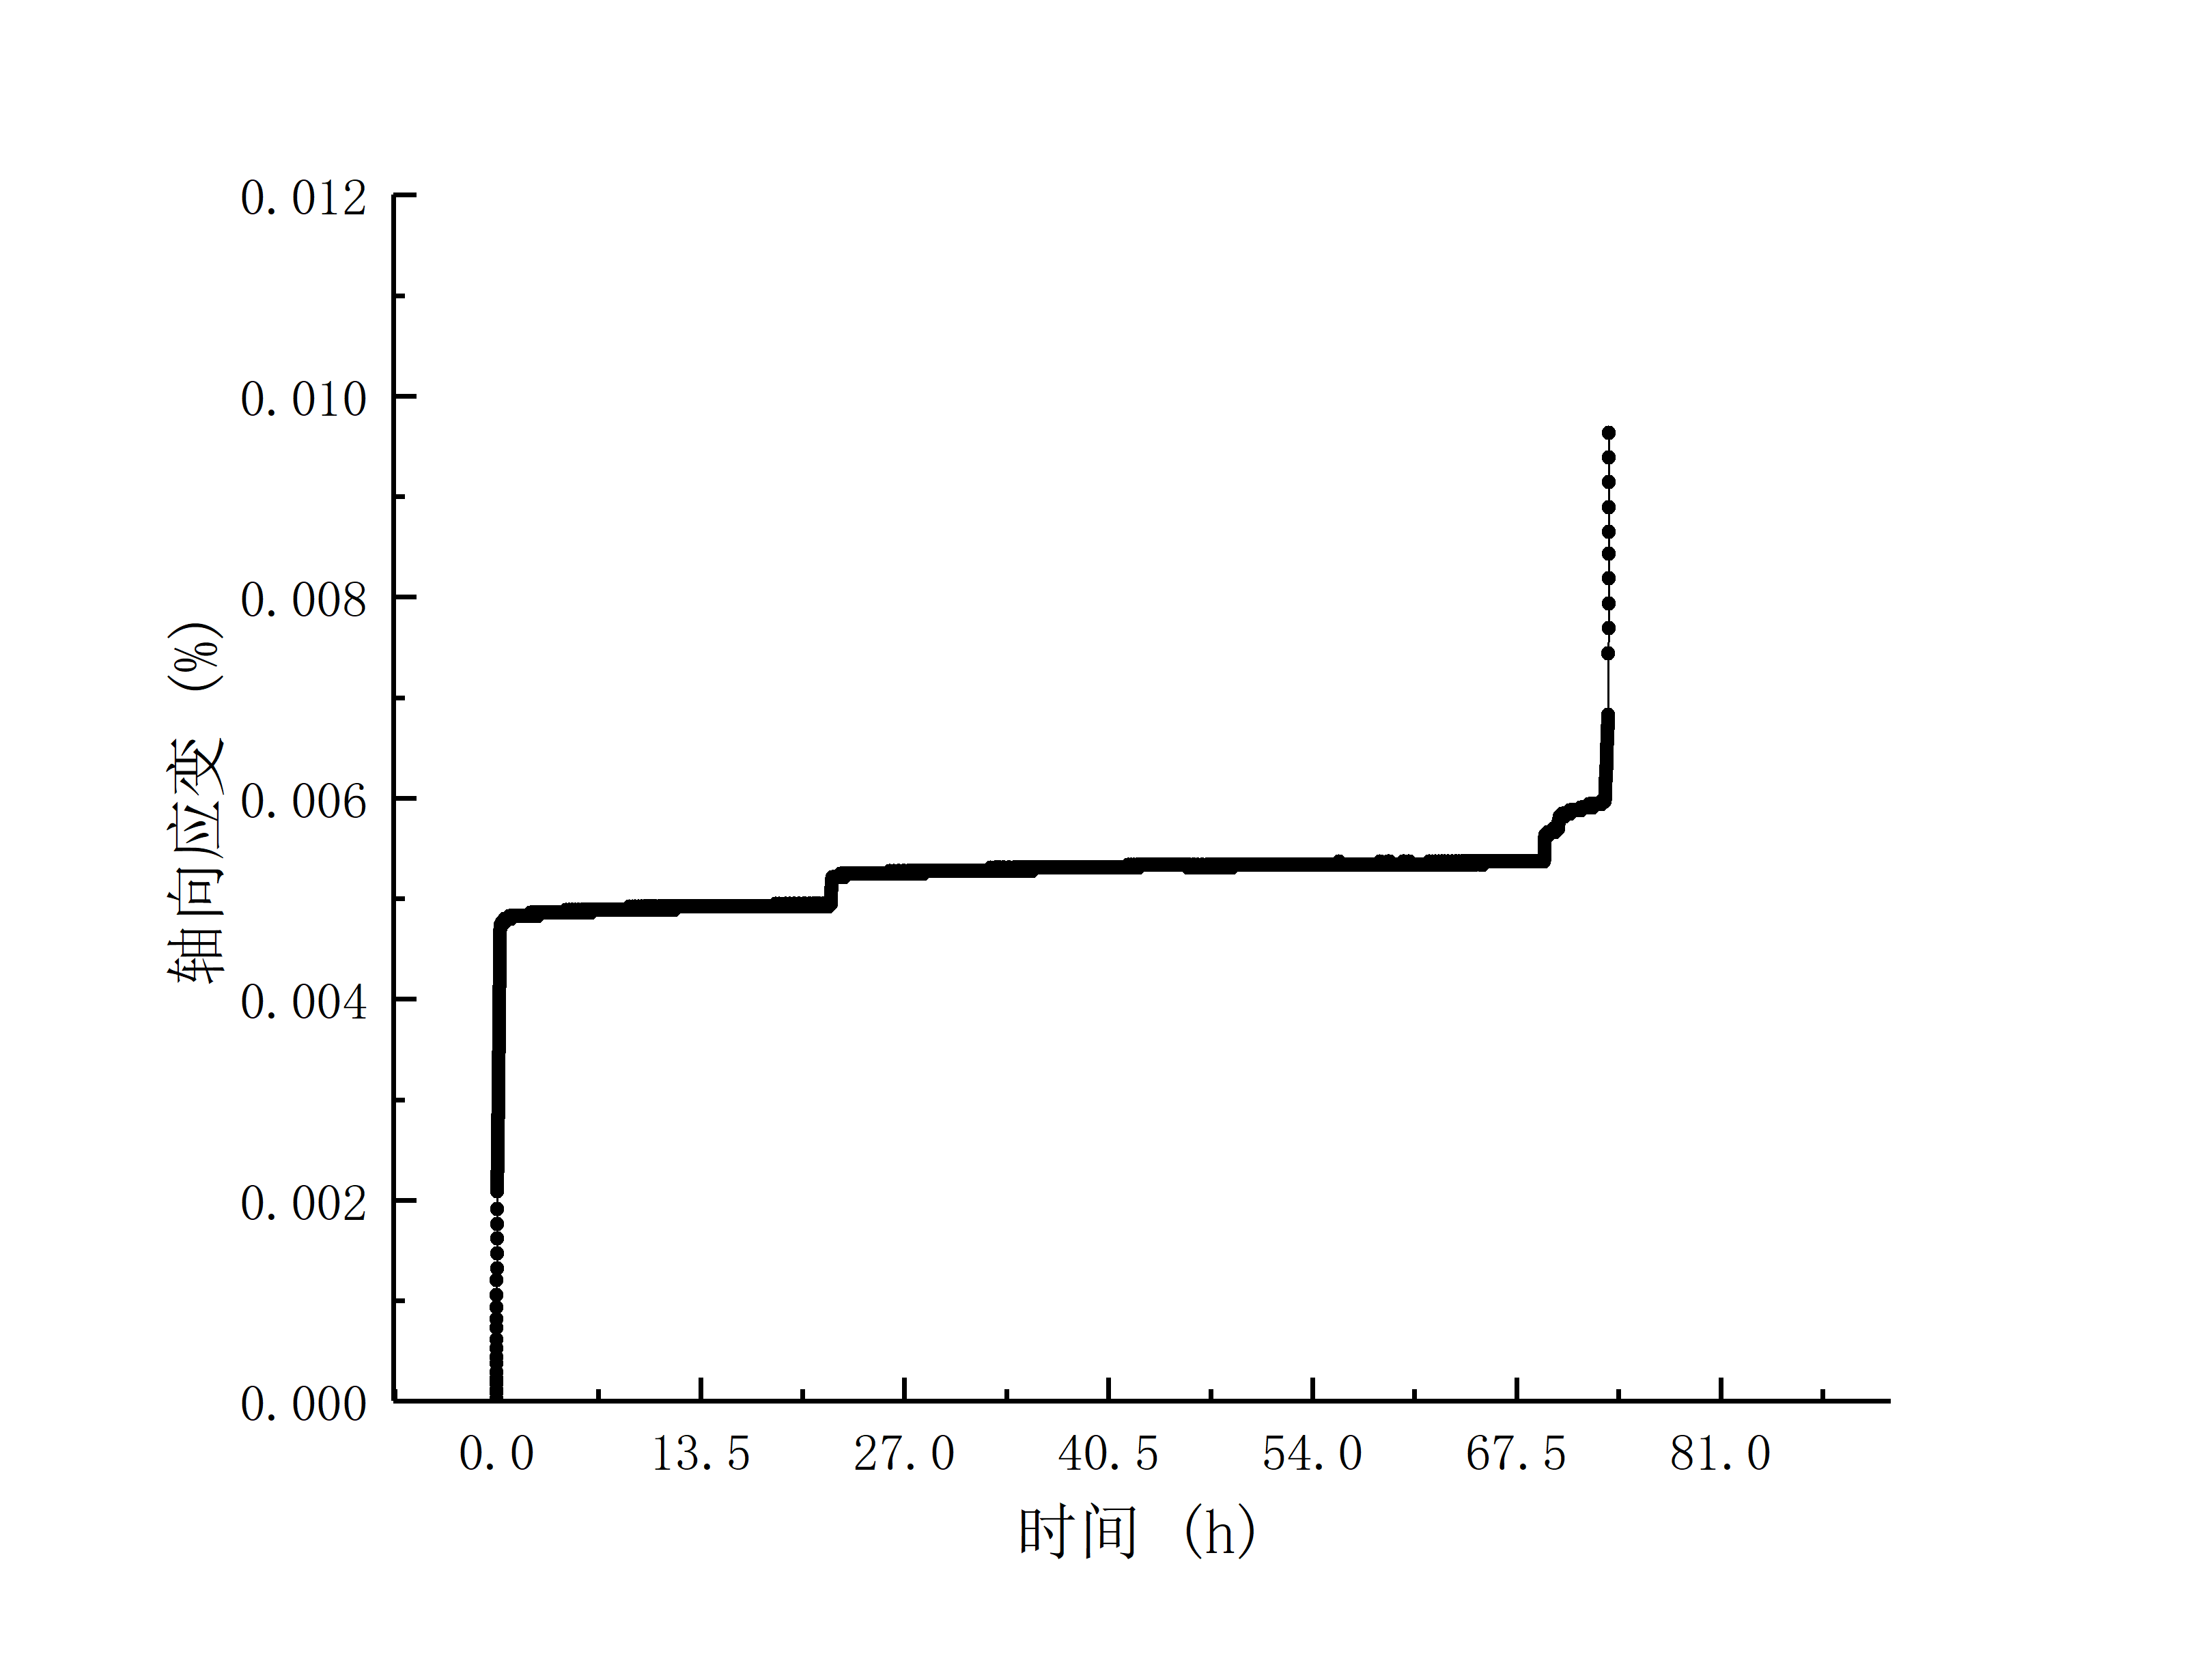
\includegraphics[width=1.2\textwidth]{img/chap2/D-01.png}
        \end{minipage}
    }
    \subfigure[D-02]
    {
        \begin{minipage}{7cm}
            \centering
            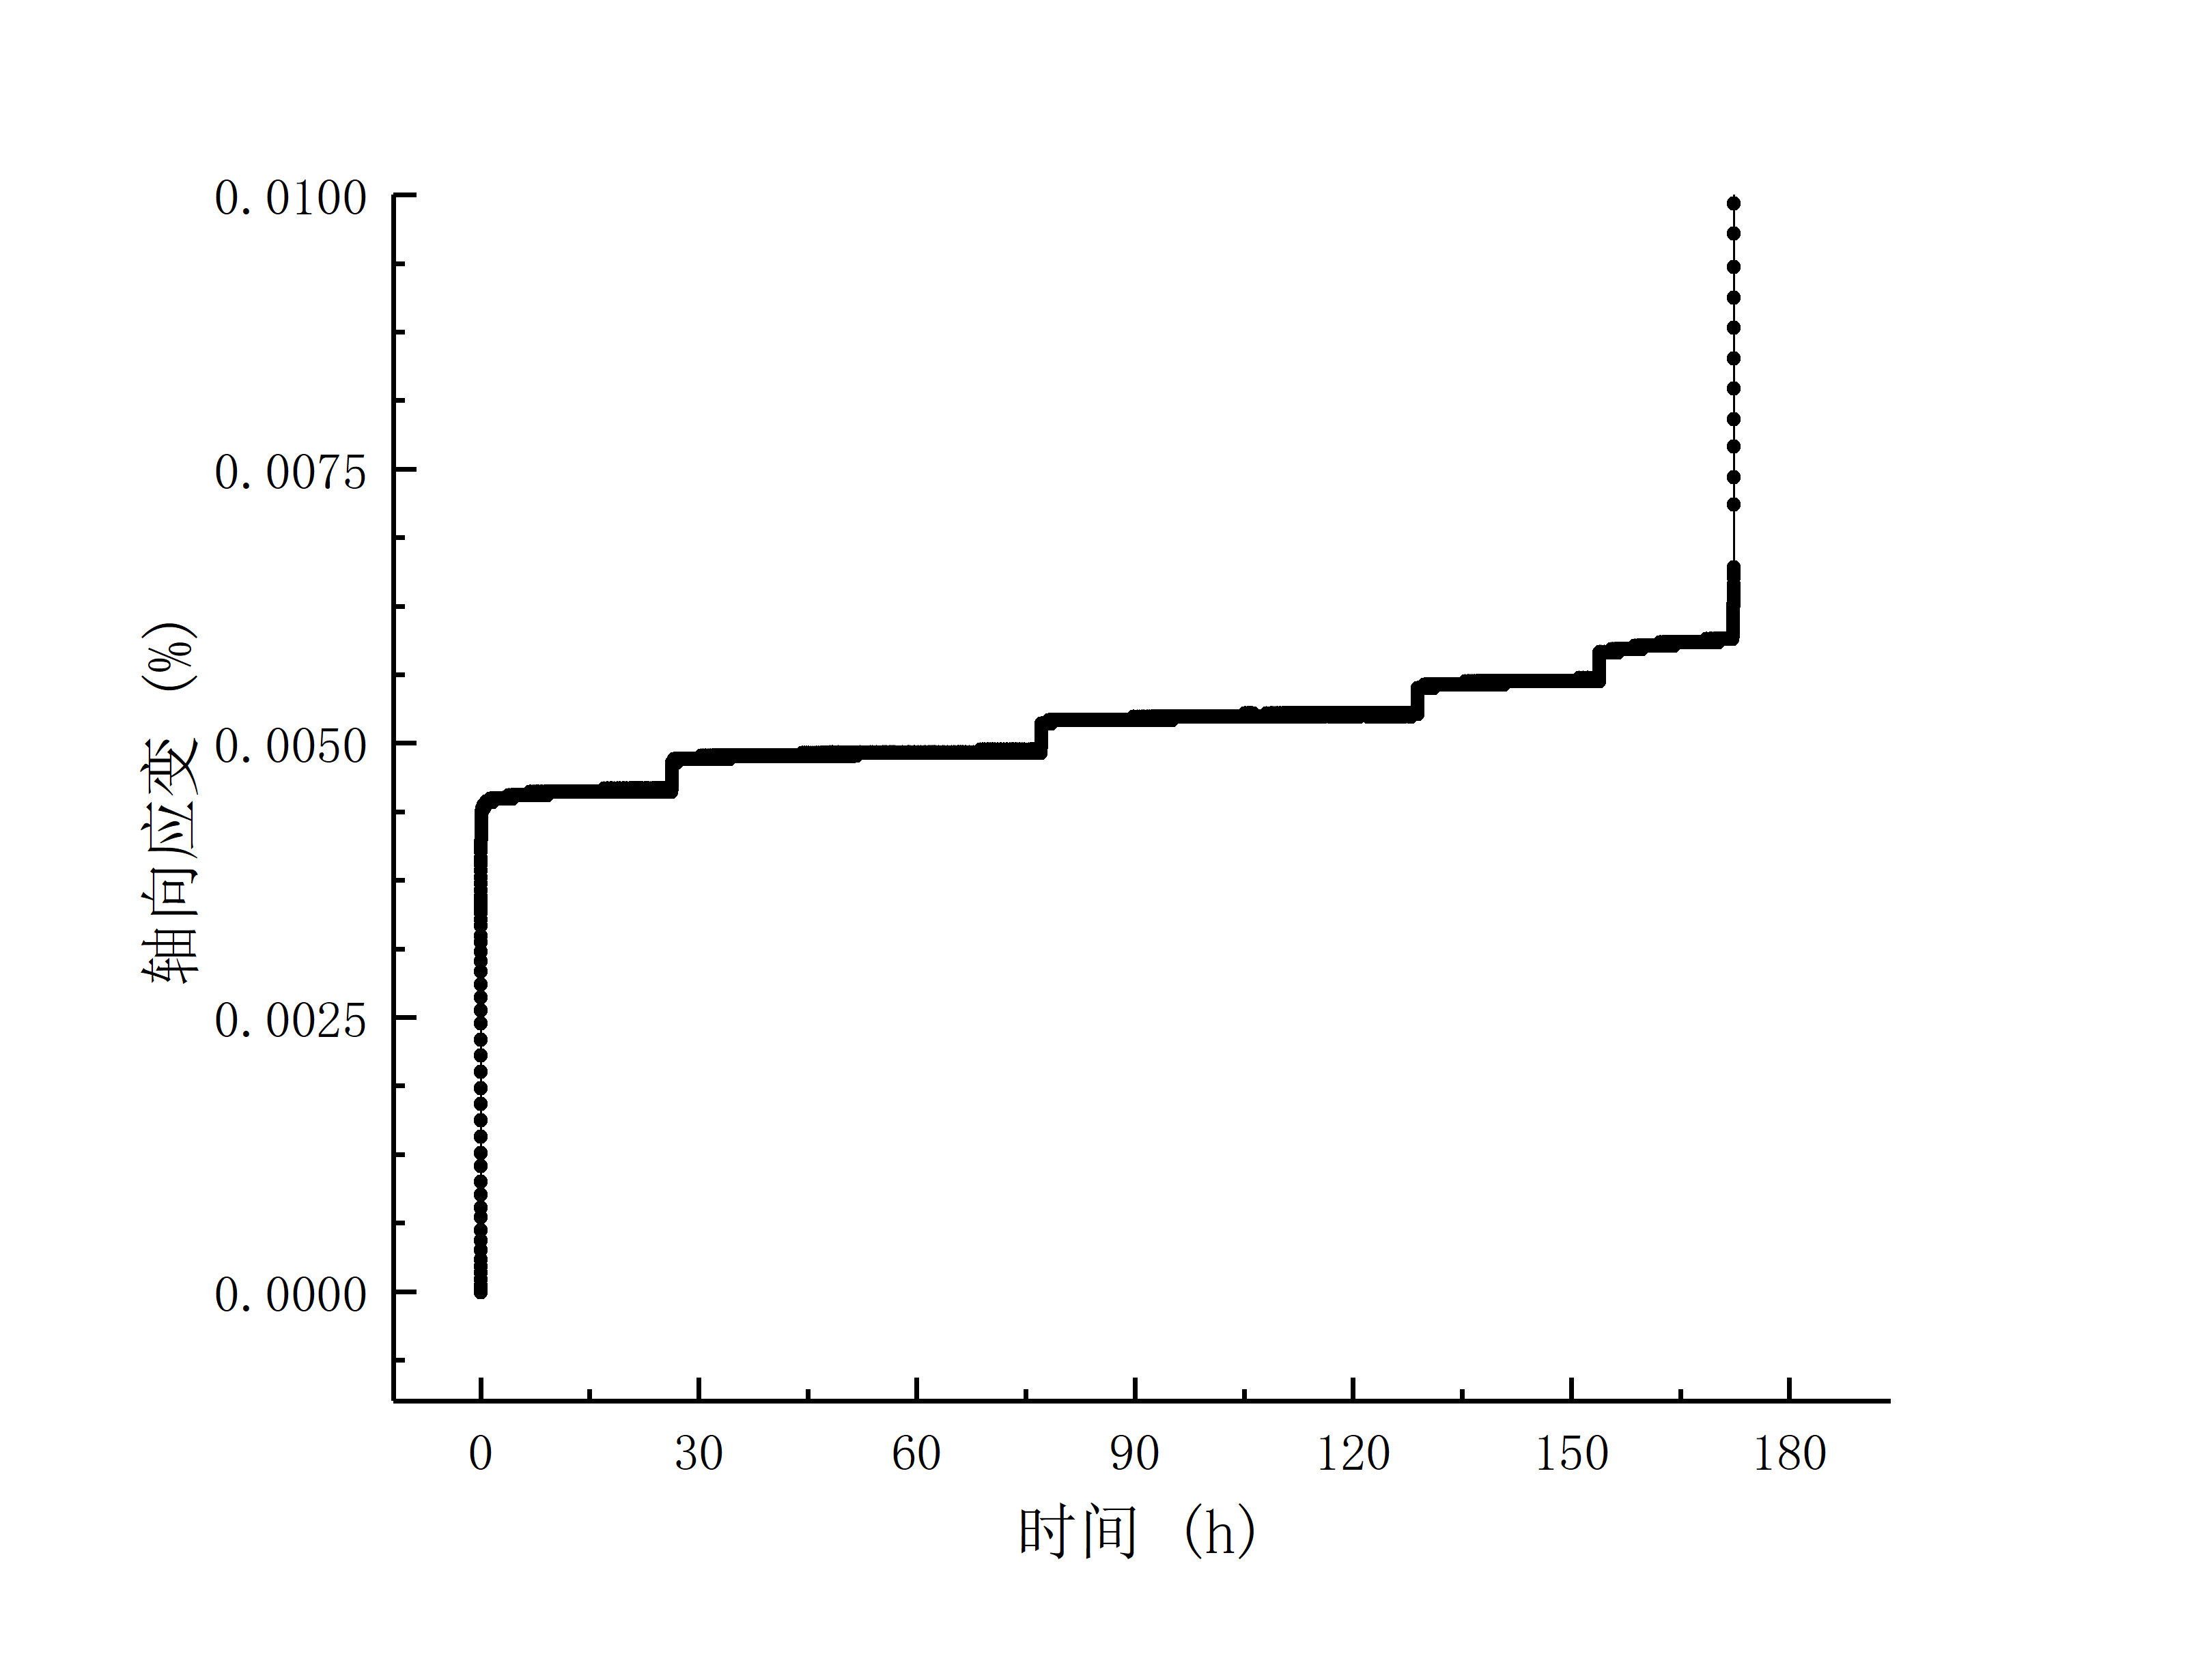
\includegraphics[width=1.2\textwidth]{img/chap2/D-02.png}
        \end{minipage}
    }
	
    \centering
    \subfigure[D-03]
    {
        \begin{minipage}{7cm}
            \centering
            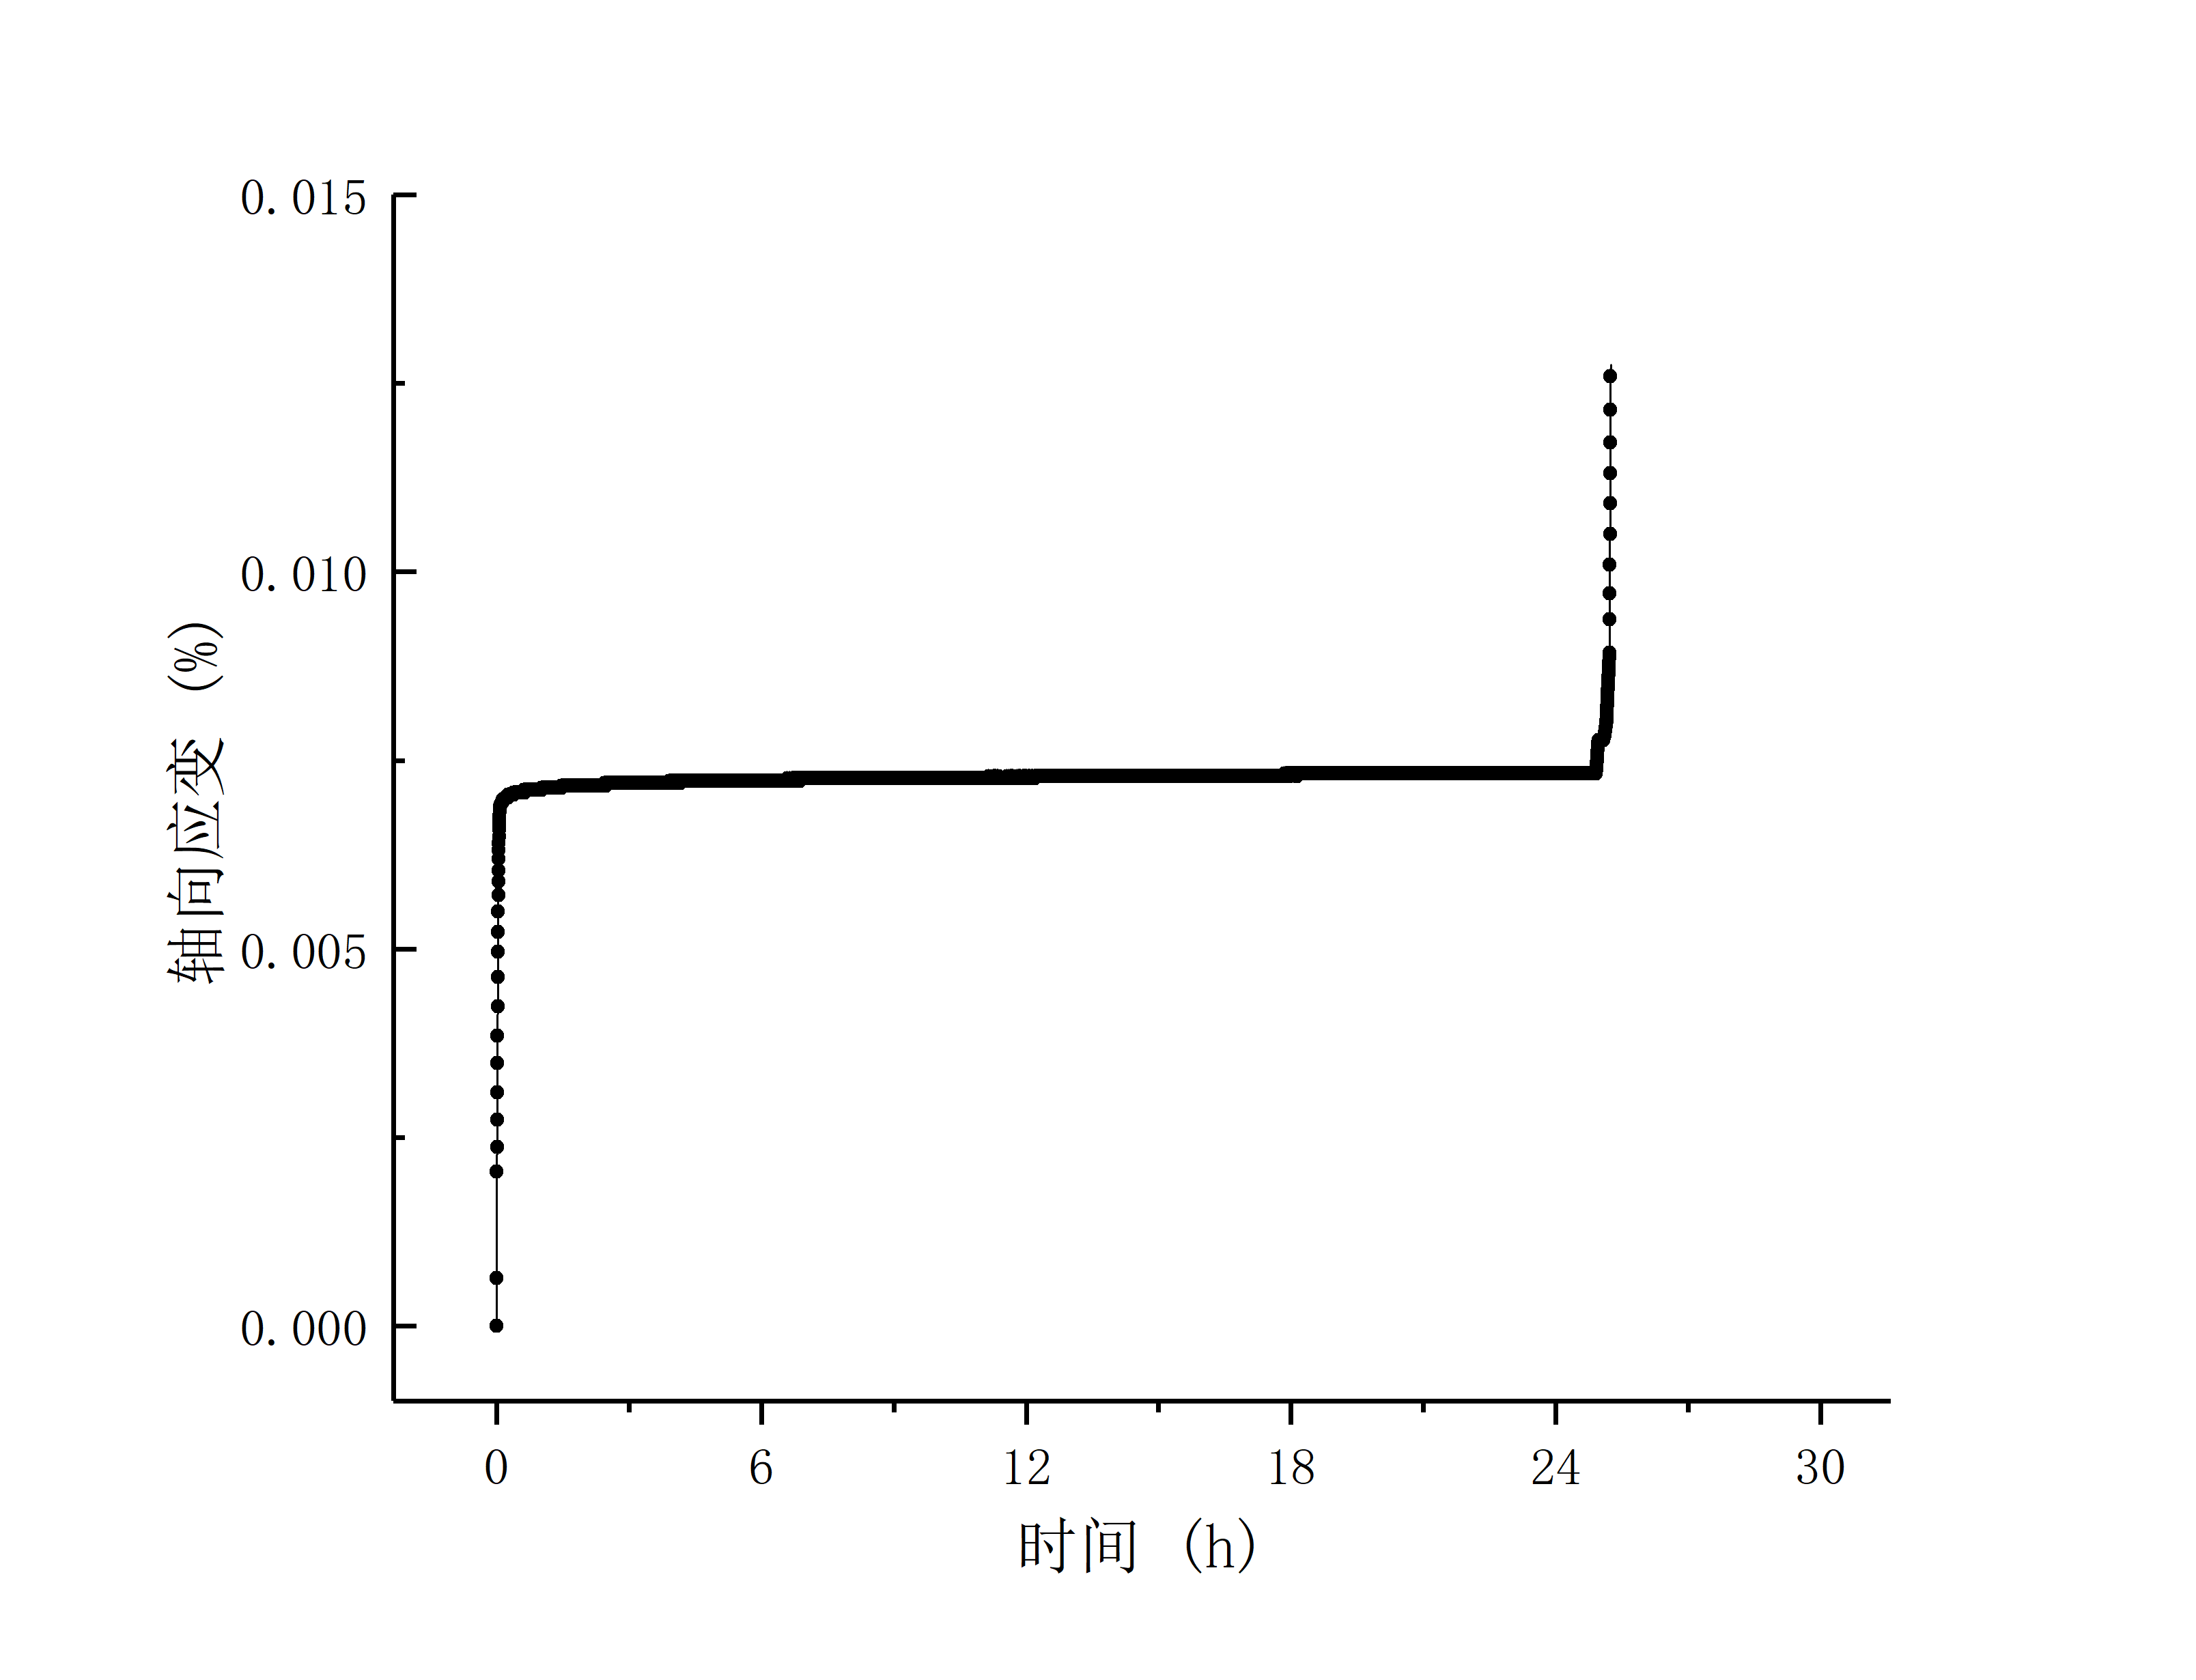
\includegraphics[width=1.2\textwidth]{img/chap2/D-03.png}
        \end{minipage}
    }
    \centering
    \caption{泥岩三轴压缩蠕变试验曲线图}
    \label{fig:2-11}
\end{figure}


\subsection{三轴流变曲线分析}
为了更好地研究泥岩的蠕变特性,更直观地观察泥岩流变曲线的变化趋势,需要将三轴流变试验中采用分级加载法的试样所得到的流变全程曲线(如图~\ref{fig:2-11})转变为一组不同应力加载等级下的分别加载流变曲线,本文采取Boltzmann叠加原理对分级加载曲线进行处理。

为了得到一组不同应力水平下的流变曲线。通常的处理方法是坐标平移法,即把每一级加载的时刻作为该级应力水平下蠕变曲线的起始时刻,而后的时间从该时刻算起,这种做法的依据就是Boltzmann叠加原理,Boltzmann叠加原理是用于线性黏弹性体的处理方法,它是描述不同时间加上不同荷载时材料的变形,该原理指出:对于蠕变过程,各级加载过程对物体变形的贡献是独立的,总的蠕变是各个加载级的蠕变的线性加和。

首先将若干个Kelvin模型串联起来,可以得到被称为广义Kelvin模型的蠕变模型,此模型响应的总应变为各元件应变之和,可以得到蠕变应变表达式如下:

\begin{equation}
     {\varepsilon(t)}={\sigma_0}(\frac{1}{E}+\frac{1}{\eta}t+\int_{0}^{\infty} \frac{1}{E(\tau)}(1-e^{-\frac{1}{\tau}t}) d{\tau})
\end{equation}

记$J_\infty=\frac{1}{E}$ ,$\Psi(t)=\int_{0}^{\infty} \frac{1}{E(\tau)}(1-e^{-\frac{1}{\tau}t}) d{\tau}$

则
\begin{equation}
     {\varepsilon(t)}={\sigma_0}(J_\infty+\frac{1}{\eta}t+\Psi(t))
\end{equation}

上式是由广义Kelvin模型积分的得到蠕变条件下蠕变变形的本构方程式,由此可以得到蠕变柔量,记为$J(t)$

\begin{equation}
J(t)=\frac{\varepsilon(t)}{\sigma_0}
    =J_\infty+\frac{1}{\eta}+\Psi(t)
\end{equation}

所示蠕变积分方程,如果在$\tau=0$时施加荷载$\sigma_0$,就可以得到该时刻的应力-应变关系:

\begin{equation}
{\varepsilon_0(t)}={\sigma_0}{J(t)}
\end{equation}

那么,在$t=\tau_1$时,施加第二个应力增量$\sigma_1$,相应的应变响应为:
\begin{equation}
{\varepsilon_1(t)}={\varepsilon(t-\tau_1)}={\sigma_1}{J(t-\tau_1)}
\end{equation}

如果将这两个应变叠加,则
\begin{equation}
     {\varepsilon(t)}={\sigma_0}{J(t)}+{\sigma_1}{J(t-\tau_1)}
\end{equation}

将该公式推广到一般情况下,在时刻$\tau_1$,$\tau_2$,$\cdots$,$\tau_n$分别施加应力增量$\sigma_1$,$\sigma_2$,$\cdots$,$\sigma_n$,则$\tau_i>0$时的应变总量即为:
\begin{equation}
     {\varepsilon(t)}=\sum_{i=0}^n\varepsilon_i(t)=\sum_{i=0}^n\sigma_iJ(t-\tau_i)
\end{equation}

若从$t_1$时刻起,应力随时间变化连续,即当时间间隔趋于无穷小时,总应变可以用下
列积分形式表达:
\begin{equation}
     {\varepsilon(t)}=\int_{0}^{\infty}J(t-\tau)\frac{\partial\sigma}{\partial\tau}d\tau
     \label{eq:2-9}
\end{equation}

式\ref{eq:2-9}说明在某时刻的变形不仅与该时刻的应力值有关,而且与应力、变形的历史有关。

我们对三轴流变试验得到的阶梯型数据曲线进行坐标平移,将每个阶段的加载过程起始点都平移至零点处,得到的曲线图如下图\ref{fig:2-10}所示。
\begin{figure}[ht!]
    \centering
    \subfigure[D-01]
    {
        \begin{minipage}{7cm}
            \centering
            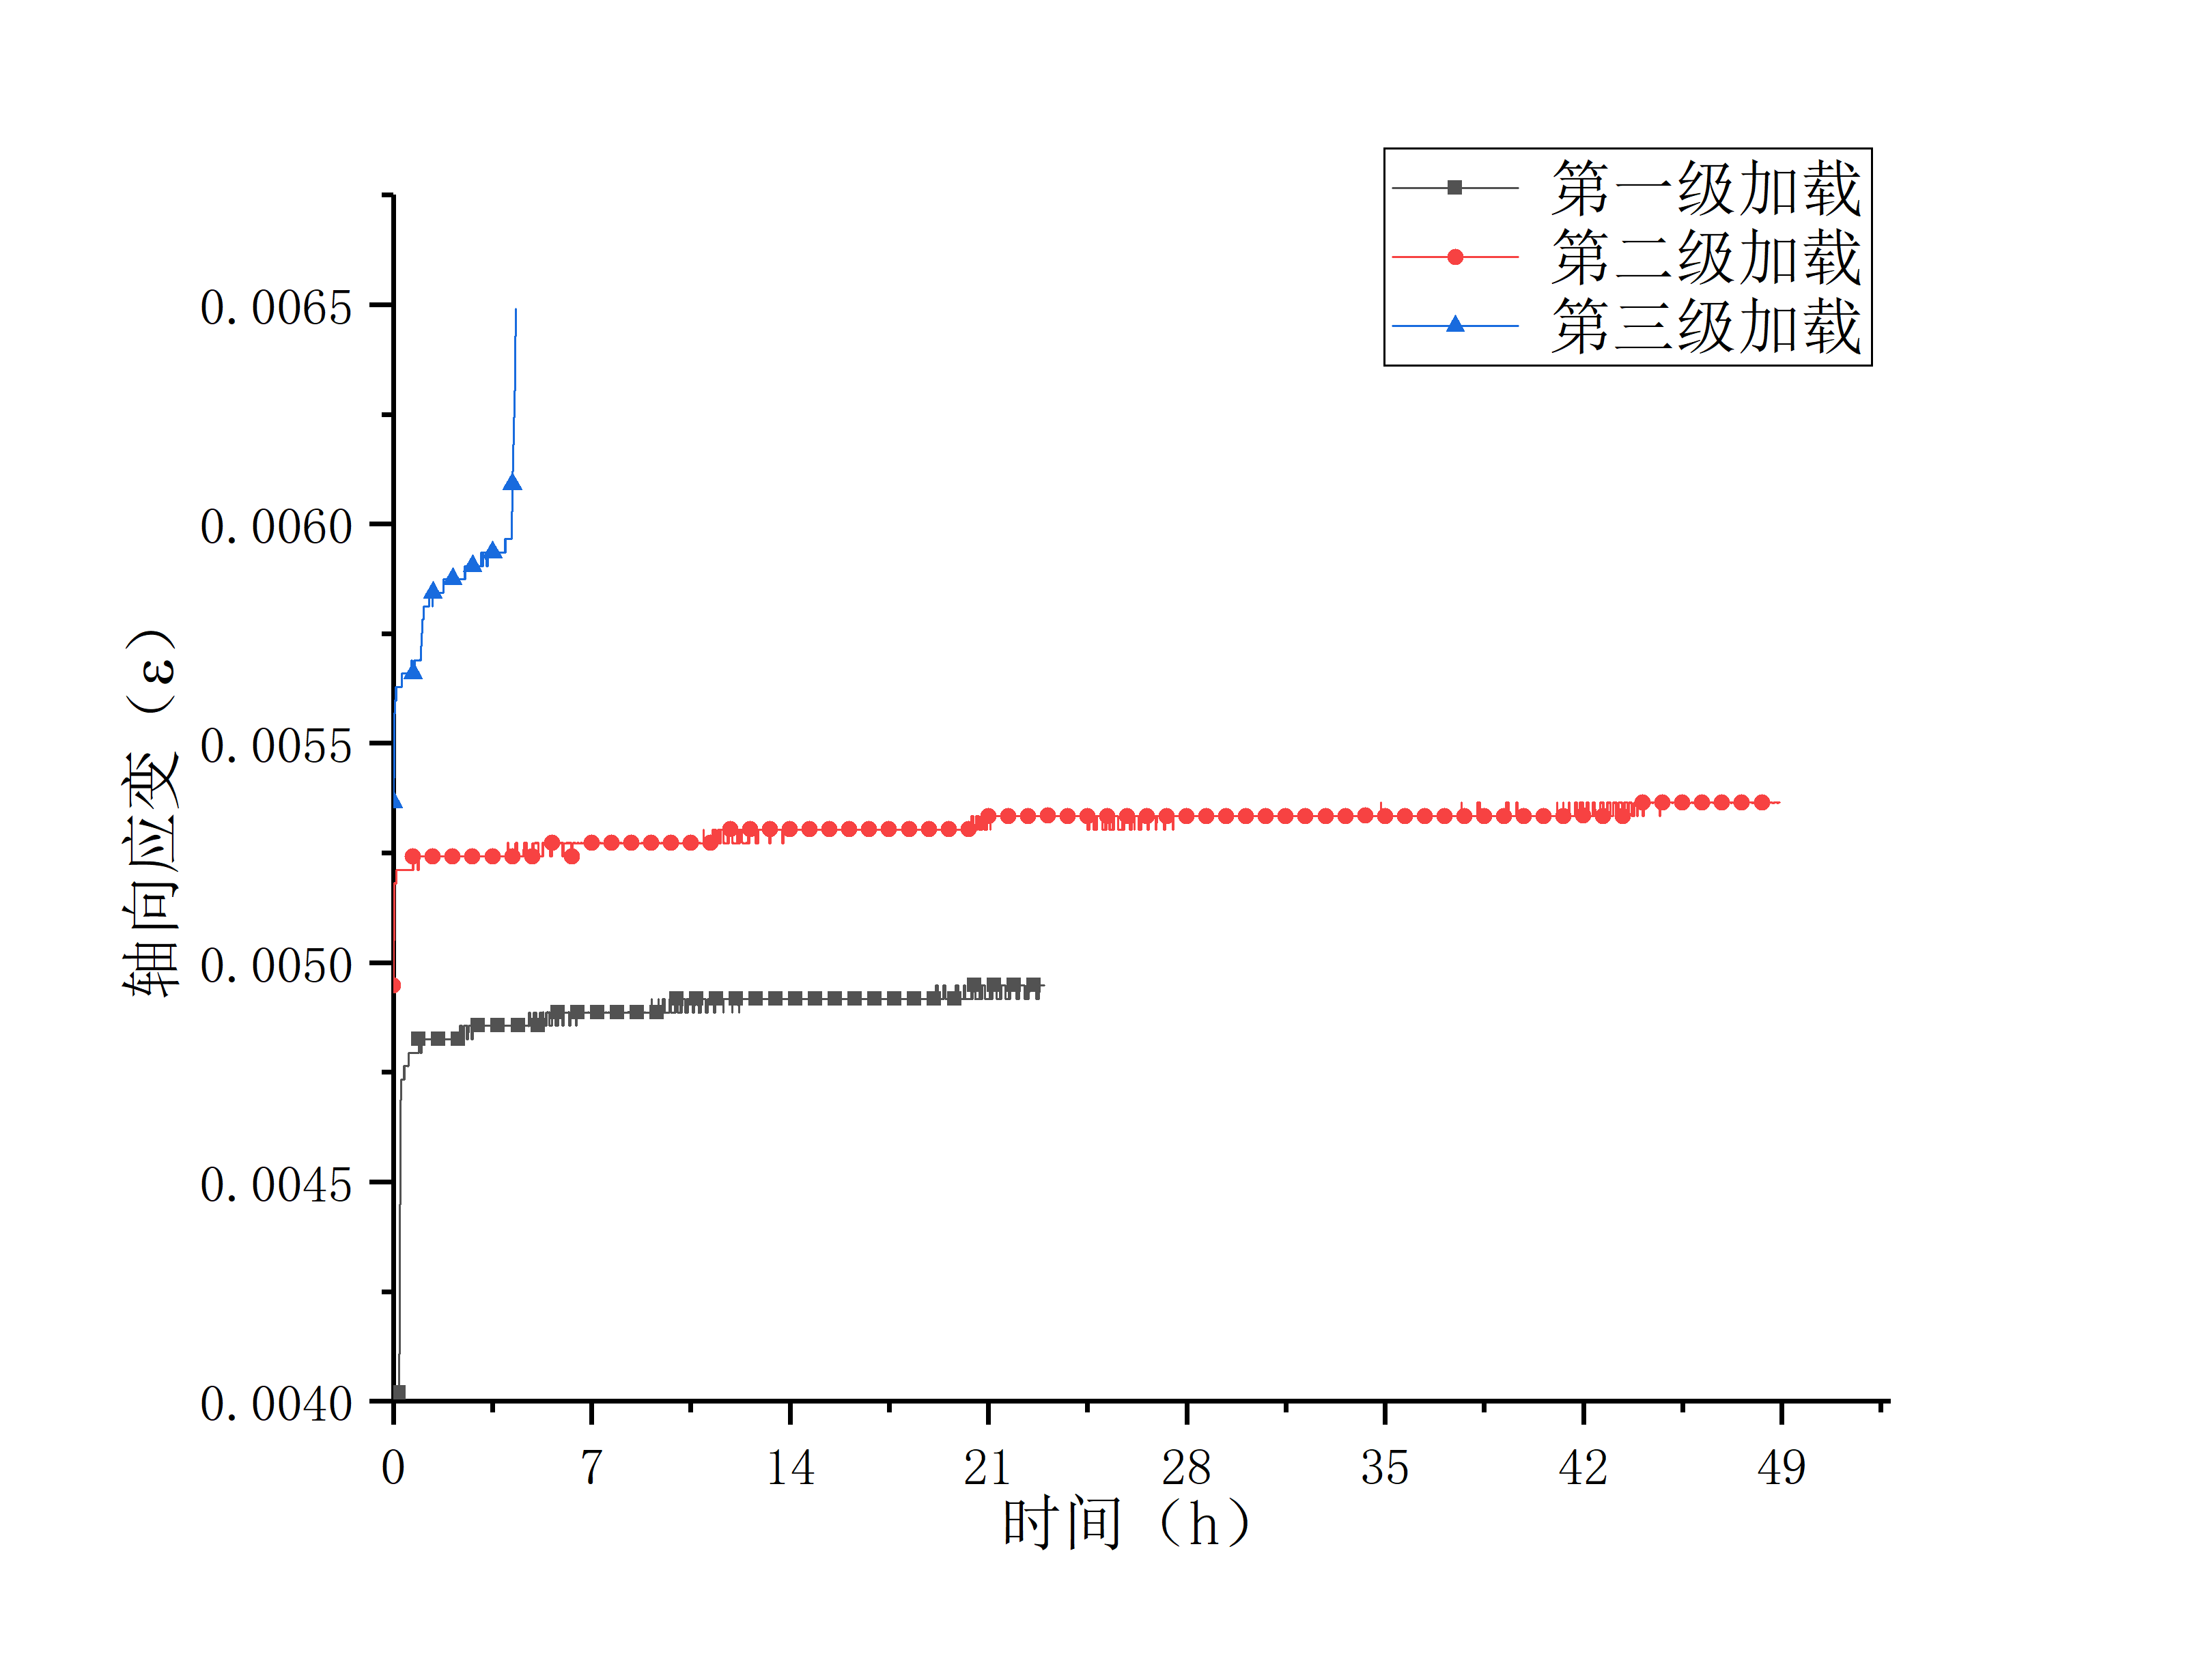
\includegraphics[width=1.2\textwidth]{img/chap2/D-01-B.png}
        \end{minipage}
    }
    \subfigure[D-02]
    {
        \begin{minipage}{7cm}
            \centering
            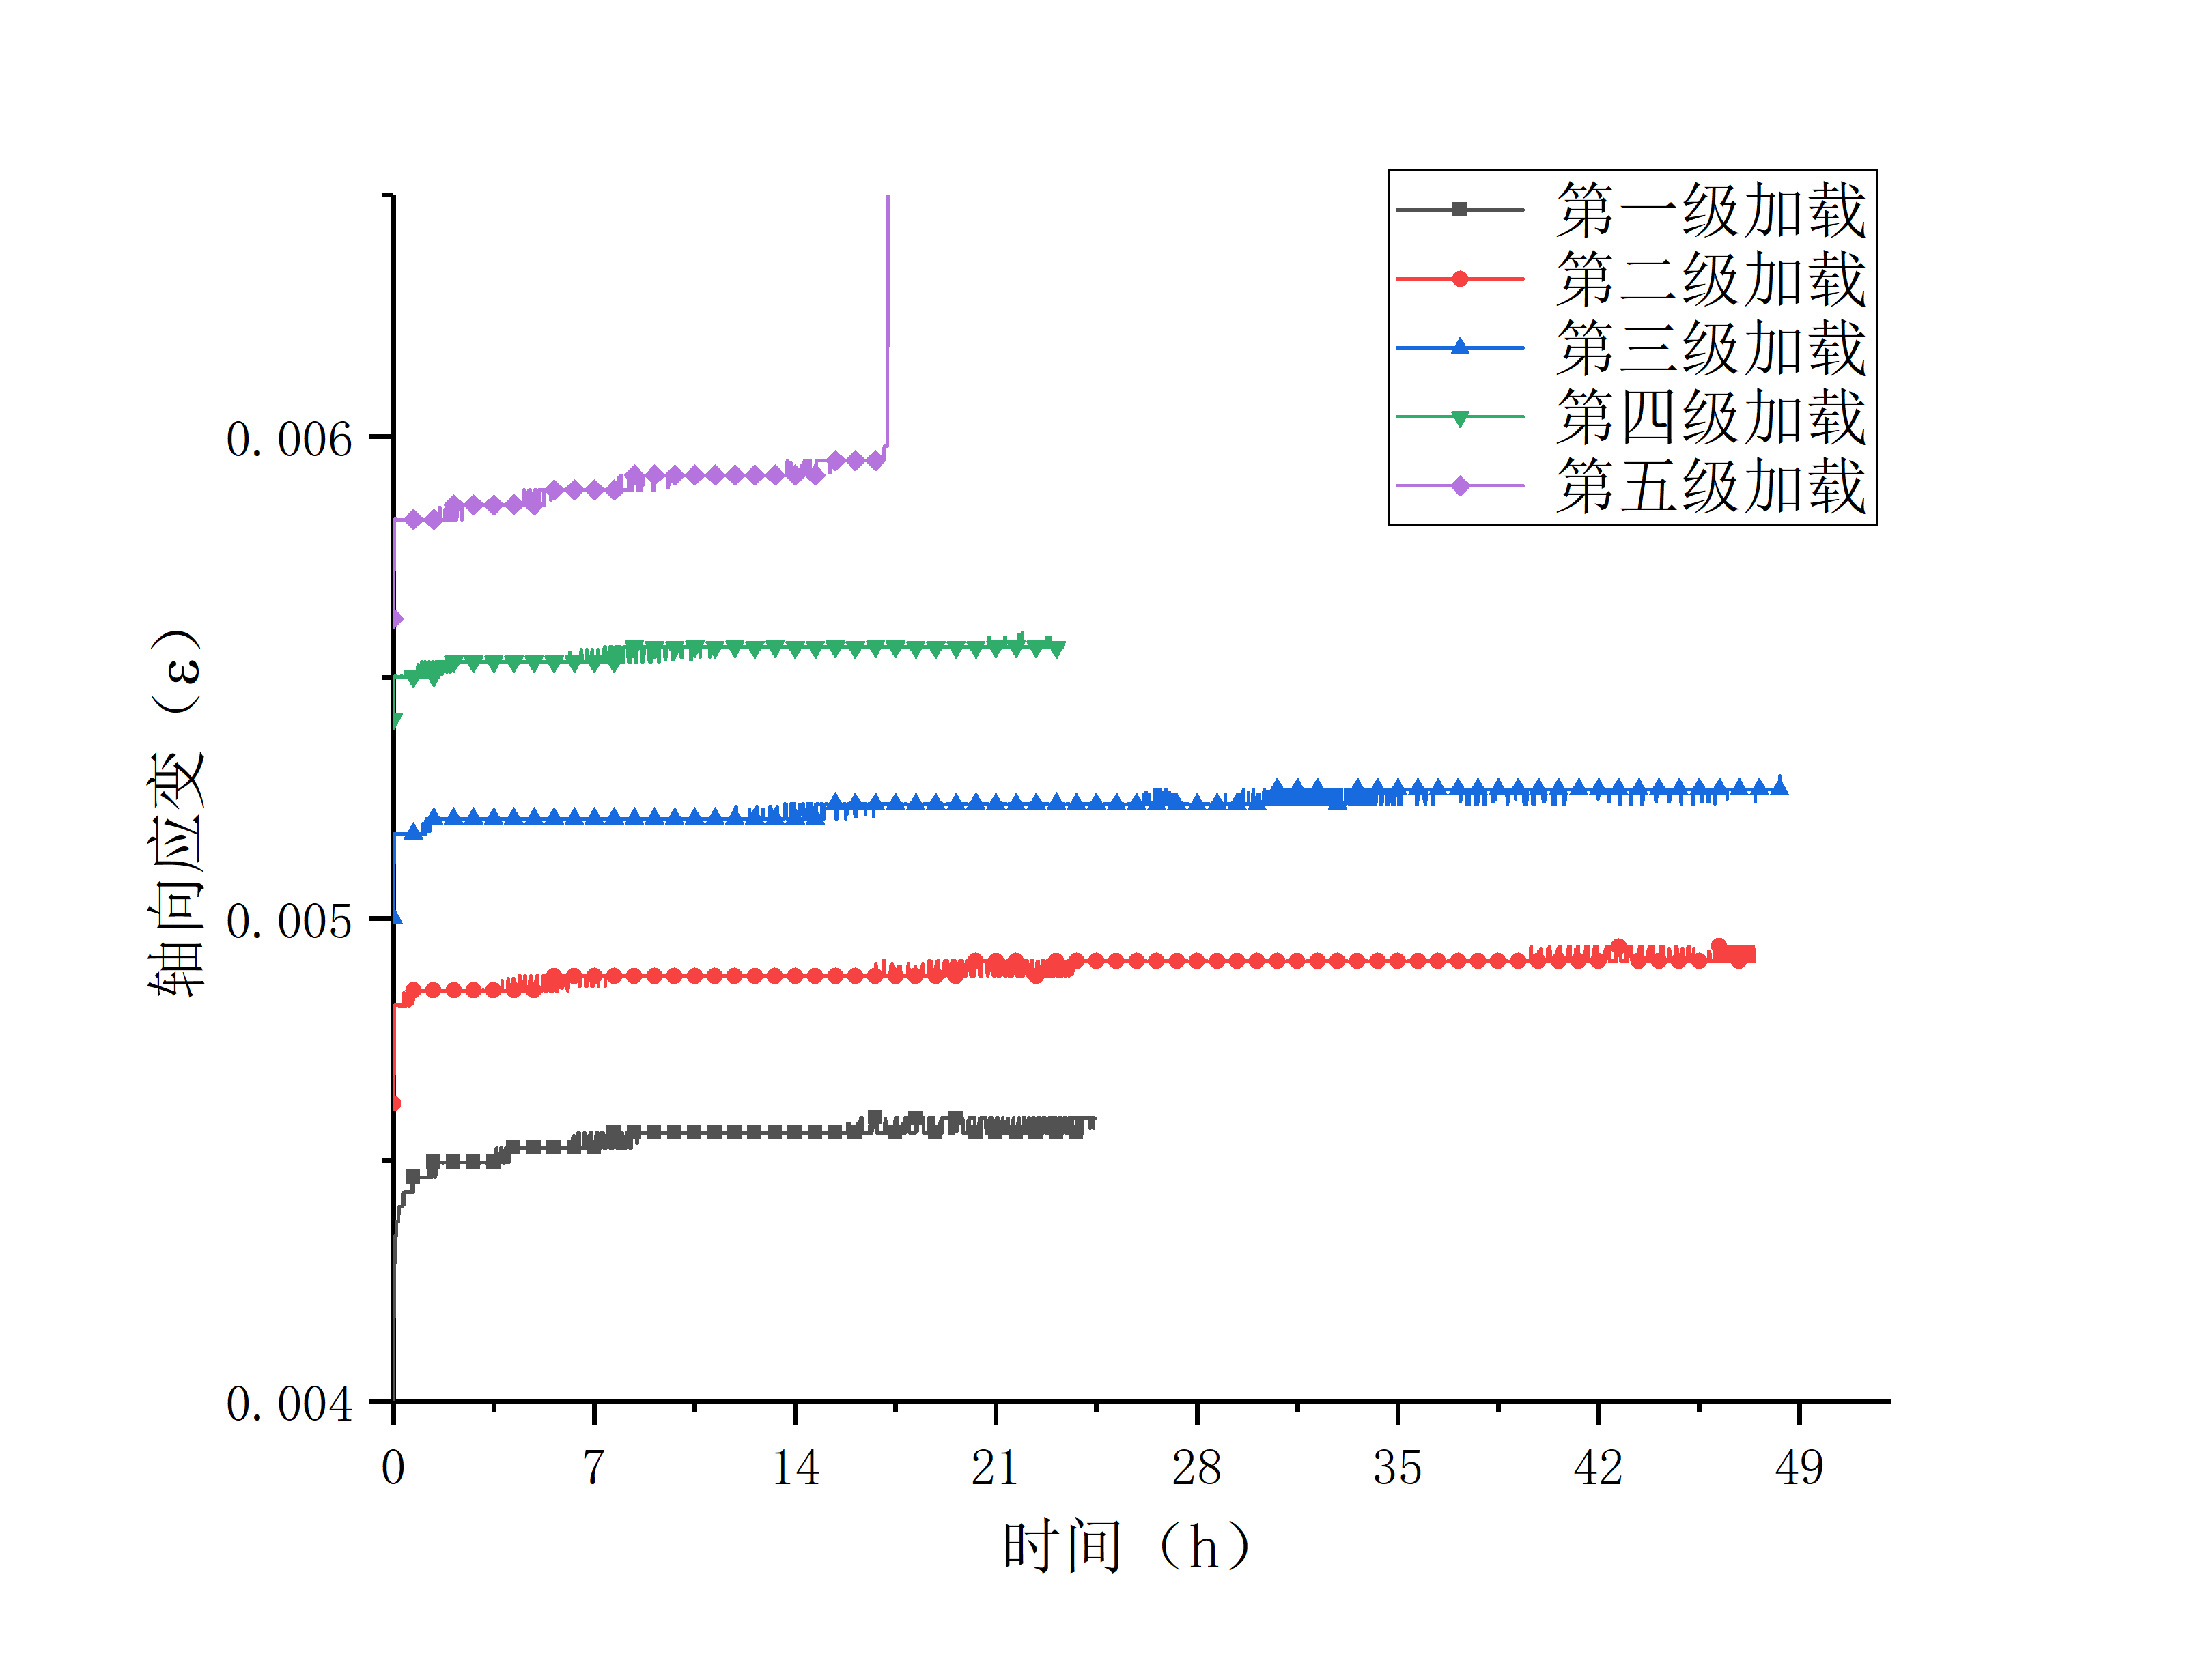
\includegraphics[width=1.2\textwidth]{img/chap2/D-02-B.png}
        \end{minipage}
    }
	
    \centering
    \subfigure[D-03]
    {
        \begin{minipage}{7cm}
            \centering
            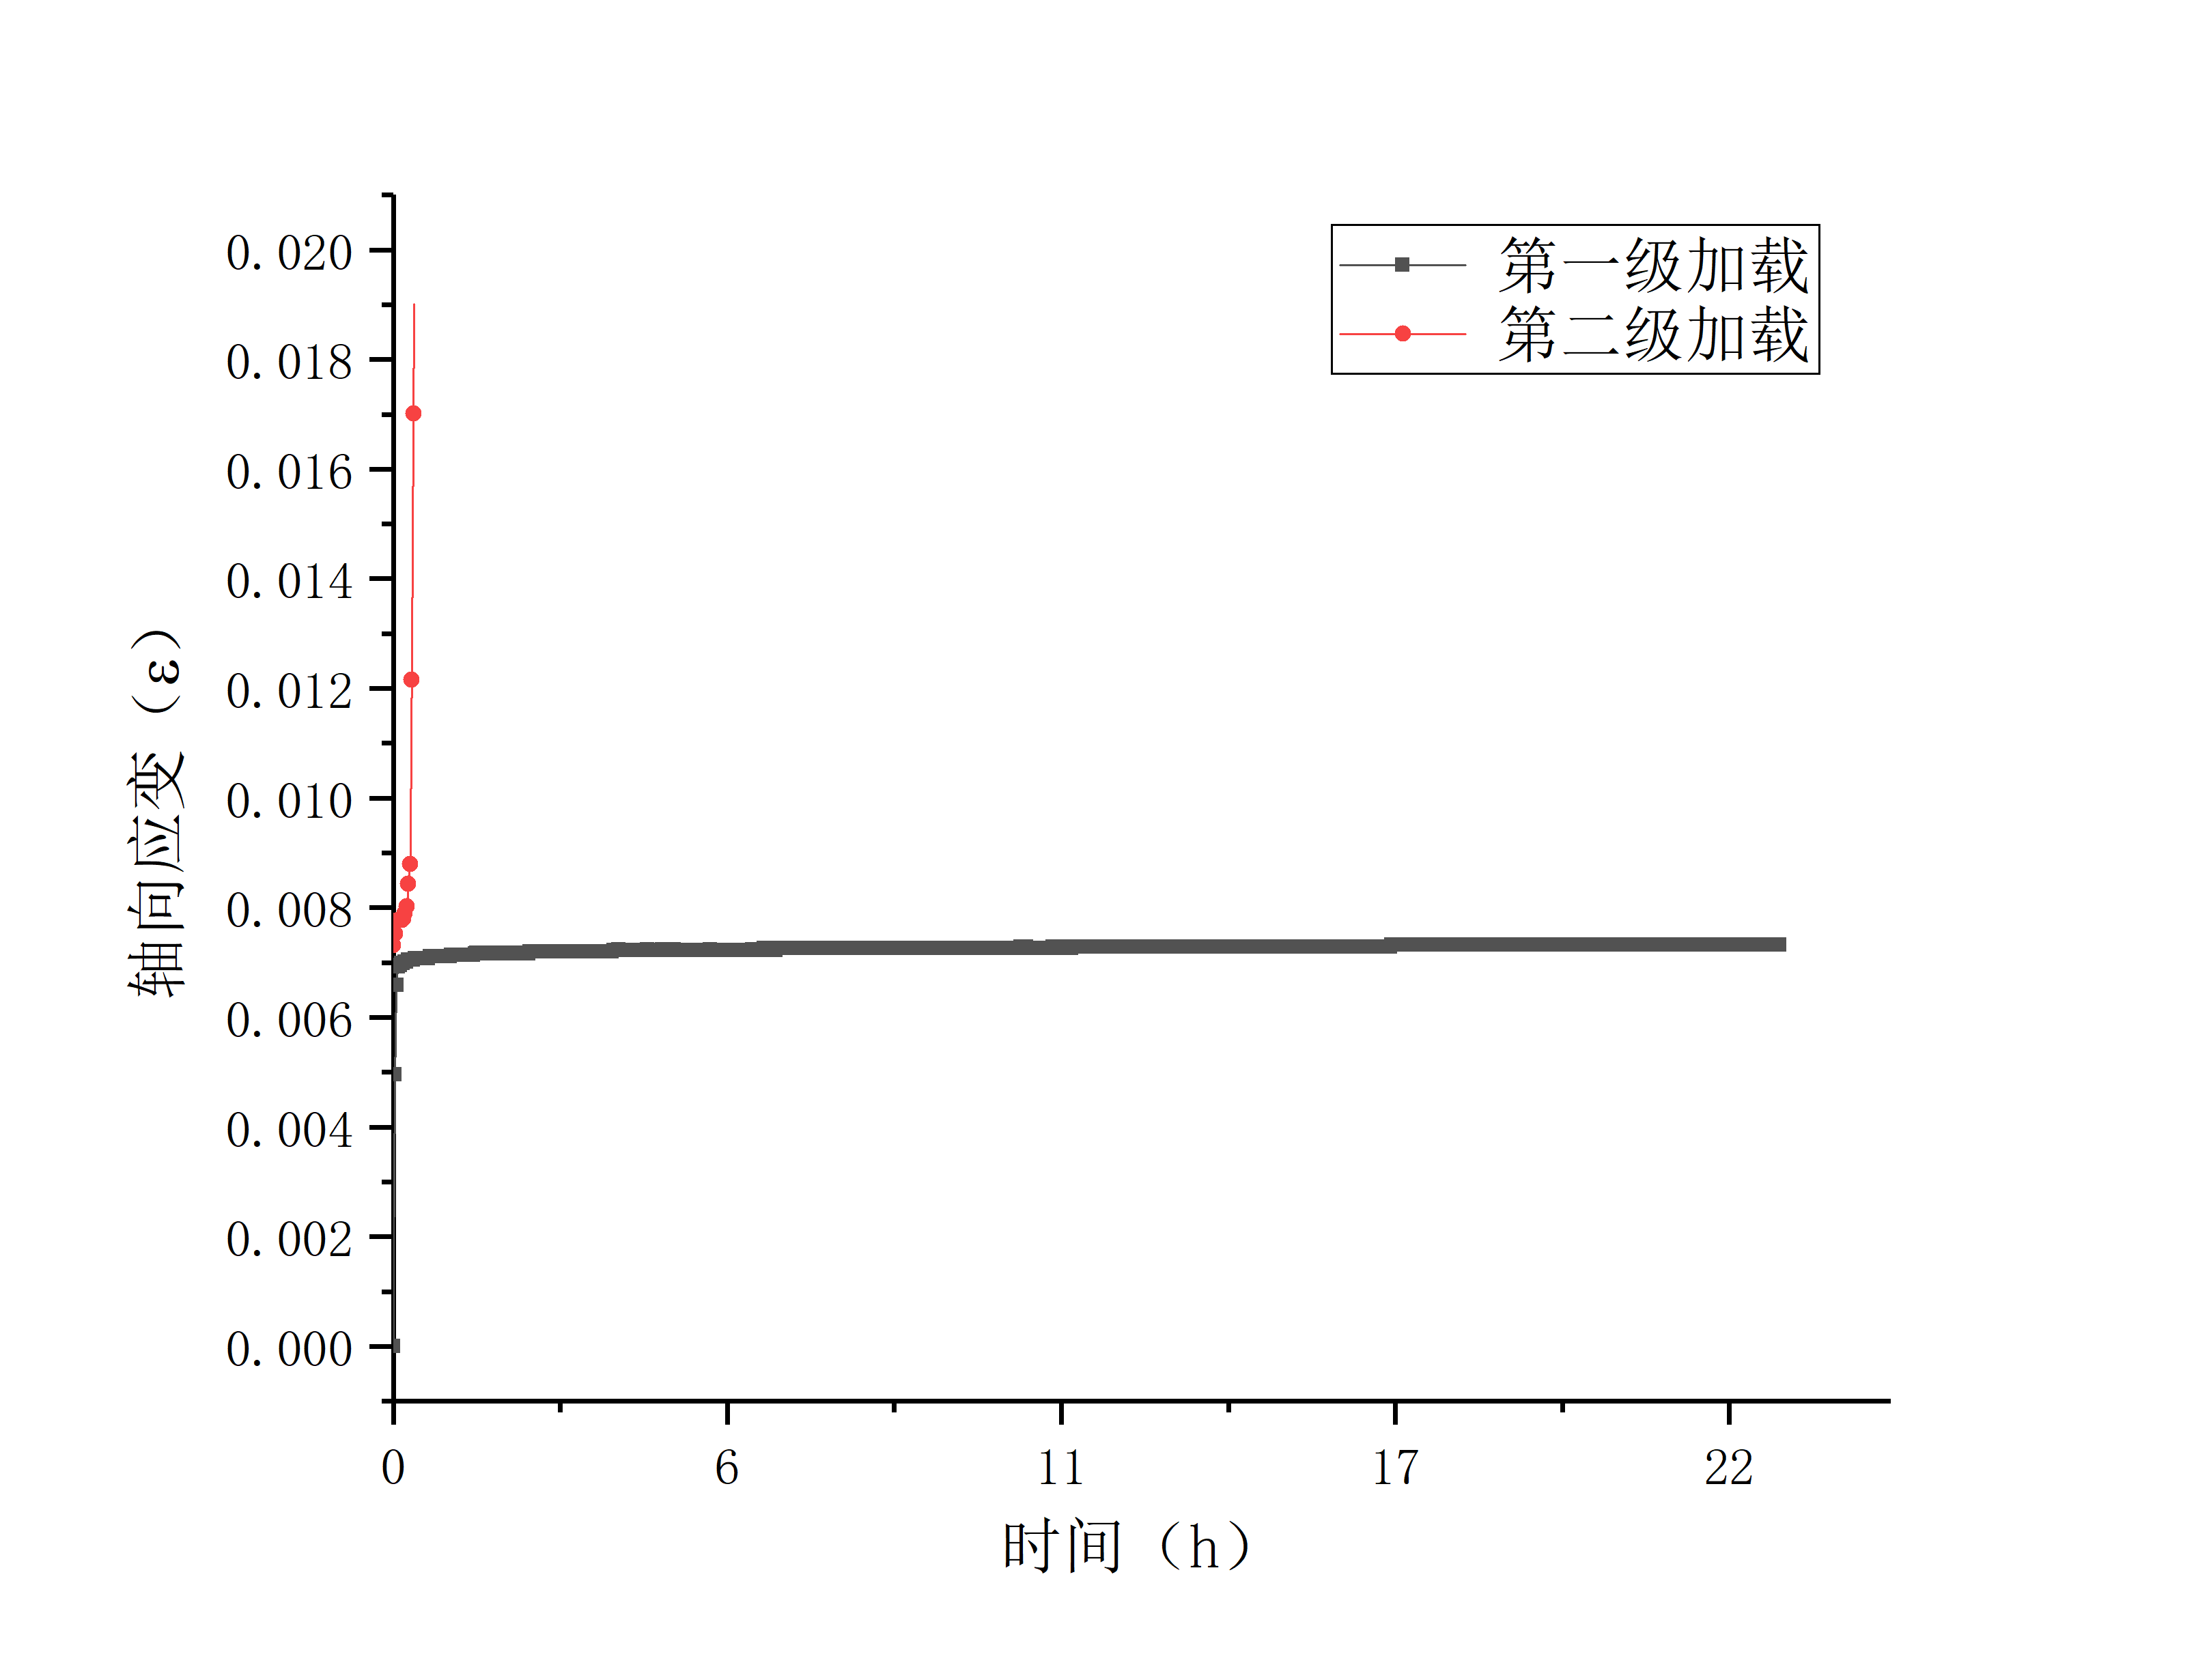
\includegraphics[width=1.2\textwidth]{img/chap2/D-03-B.png}
        \end{minipage}
    }
    \centering
    \caption{泥岩流变试验同围压下各级加载曲线图}
    \label{fig:2-12}
\end{figure}

考虑在同一围压下不同加载等级下的流变曲线,由图\ref{fig:2-12}可知:

(1)在同一围压下的泥岩试样流变曲线中,试样在加载的瞬间都会产生瞬时变形,不过由于本次采用的是分级加载的方式,而不是分级加卸载的试验形式,因此从第二级架子开始的瞬时轴向应变普遍较小。随着应力等级的提升,试样的流变速率也随之增大,说明应力水平越高,泥岩试样的流变特性越明显。

(2)在较低的应力等级下,岩石以瞬时变形为主,流变变形量较小。例如,在\SI{10}{MPa}的围压下,第一级应力加载时,达到稳定蠕变阶段时,瞬时轴向应增加了0.0045,而在之后的流变阶段,仅产生了0.00009的轴向应变;而在第五级应力的加载下,则产生了0.00015的瞬时应变和0.00015的流变应变,随着加载应力的提升,流变变形比重逐渐增大。

(3)在流变过程中,在较低的应力等级下,岩石以瞬时变形为主,流变变形量较小,在经历一定时间后流变变形量收敛,趋于定值,流变变形速率减小到无限趋近于零,在经过一段时间后,试样应变不再增加,趋于一个稳定的值;而当应力等级较高时,在经历一定时间后,流变变形速率趋于某一不为零的定值,流变速率保持不变,试样轴向应变随着时间呈线性增长,这一点从图 2.9(b) 中可以较为清楚的看到。

(4)泥岩试样的三轴流变试验结果表明,该泥岩具有较为显著的流变特性,且在流变过程中,较长时间都处于稳定蠕变阶段。不过,在本次进行的三组三轴流变试验都没有完成预期的加载目标,D-01完成了两组加载等级,在第三级加载时试样就已经破坏,D-03则是只完成了一组加载,第二级加载开始后试样便迅速破坏了,仅有第二组D-02加载到了第五级,综合常规三轴压缩试验的结果,这主要是由于试样强度不够均匀,通过压缩试验选取的应力加载水平过大。

(5)在流变曲线中,我们发现应变在某些阶段会上下波动,这与单轴流变试验的曲线波动原因是一致的,都是因为试样内部存在的微小裂缝对试验数据造成的一些可以忽略不计的影响。


\subsection{加速流变阶段分析}
在三轴流变试验中我们发现了一个在单轴流变试验中未曾出现过的流变阶段——加速流变阶段。在分级加载的最后一级应力水平下,岩石流变变形表现出与以往应力水平不同的时效特征。三轴流变过程中最后一级加载下流变变形及流变速率如图\ref{fig:2-11}所示。

\begin{figure}[ht!]
    \centering
    \subfigure[D-01]
    {
        \begin{minipage}{7cm}
            \centering
            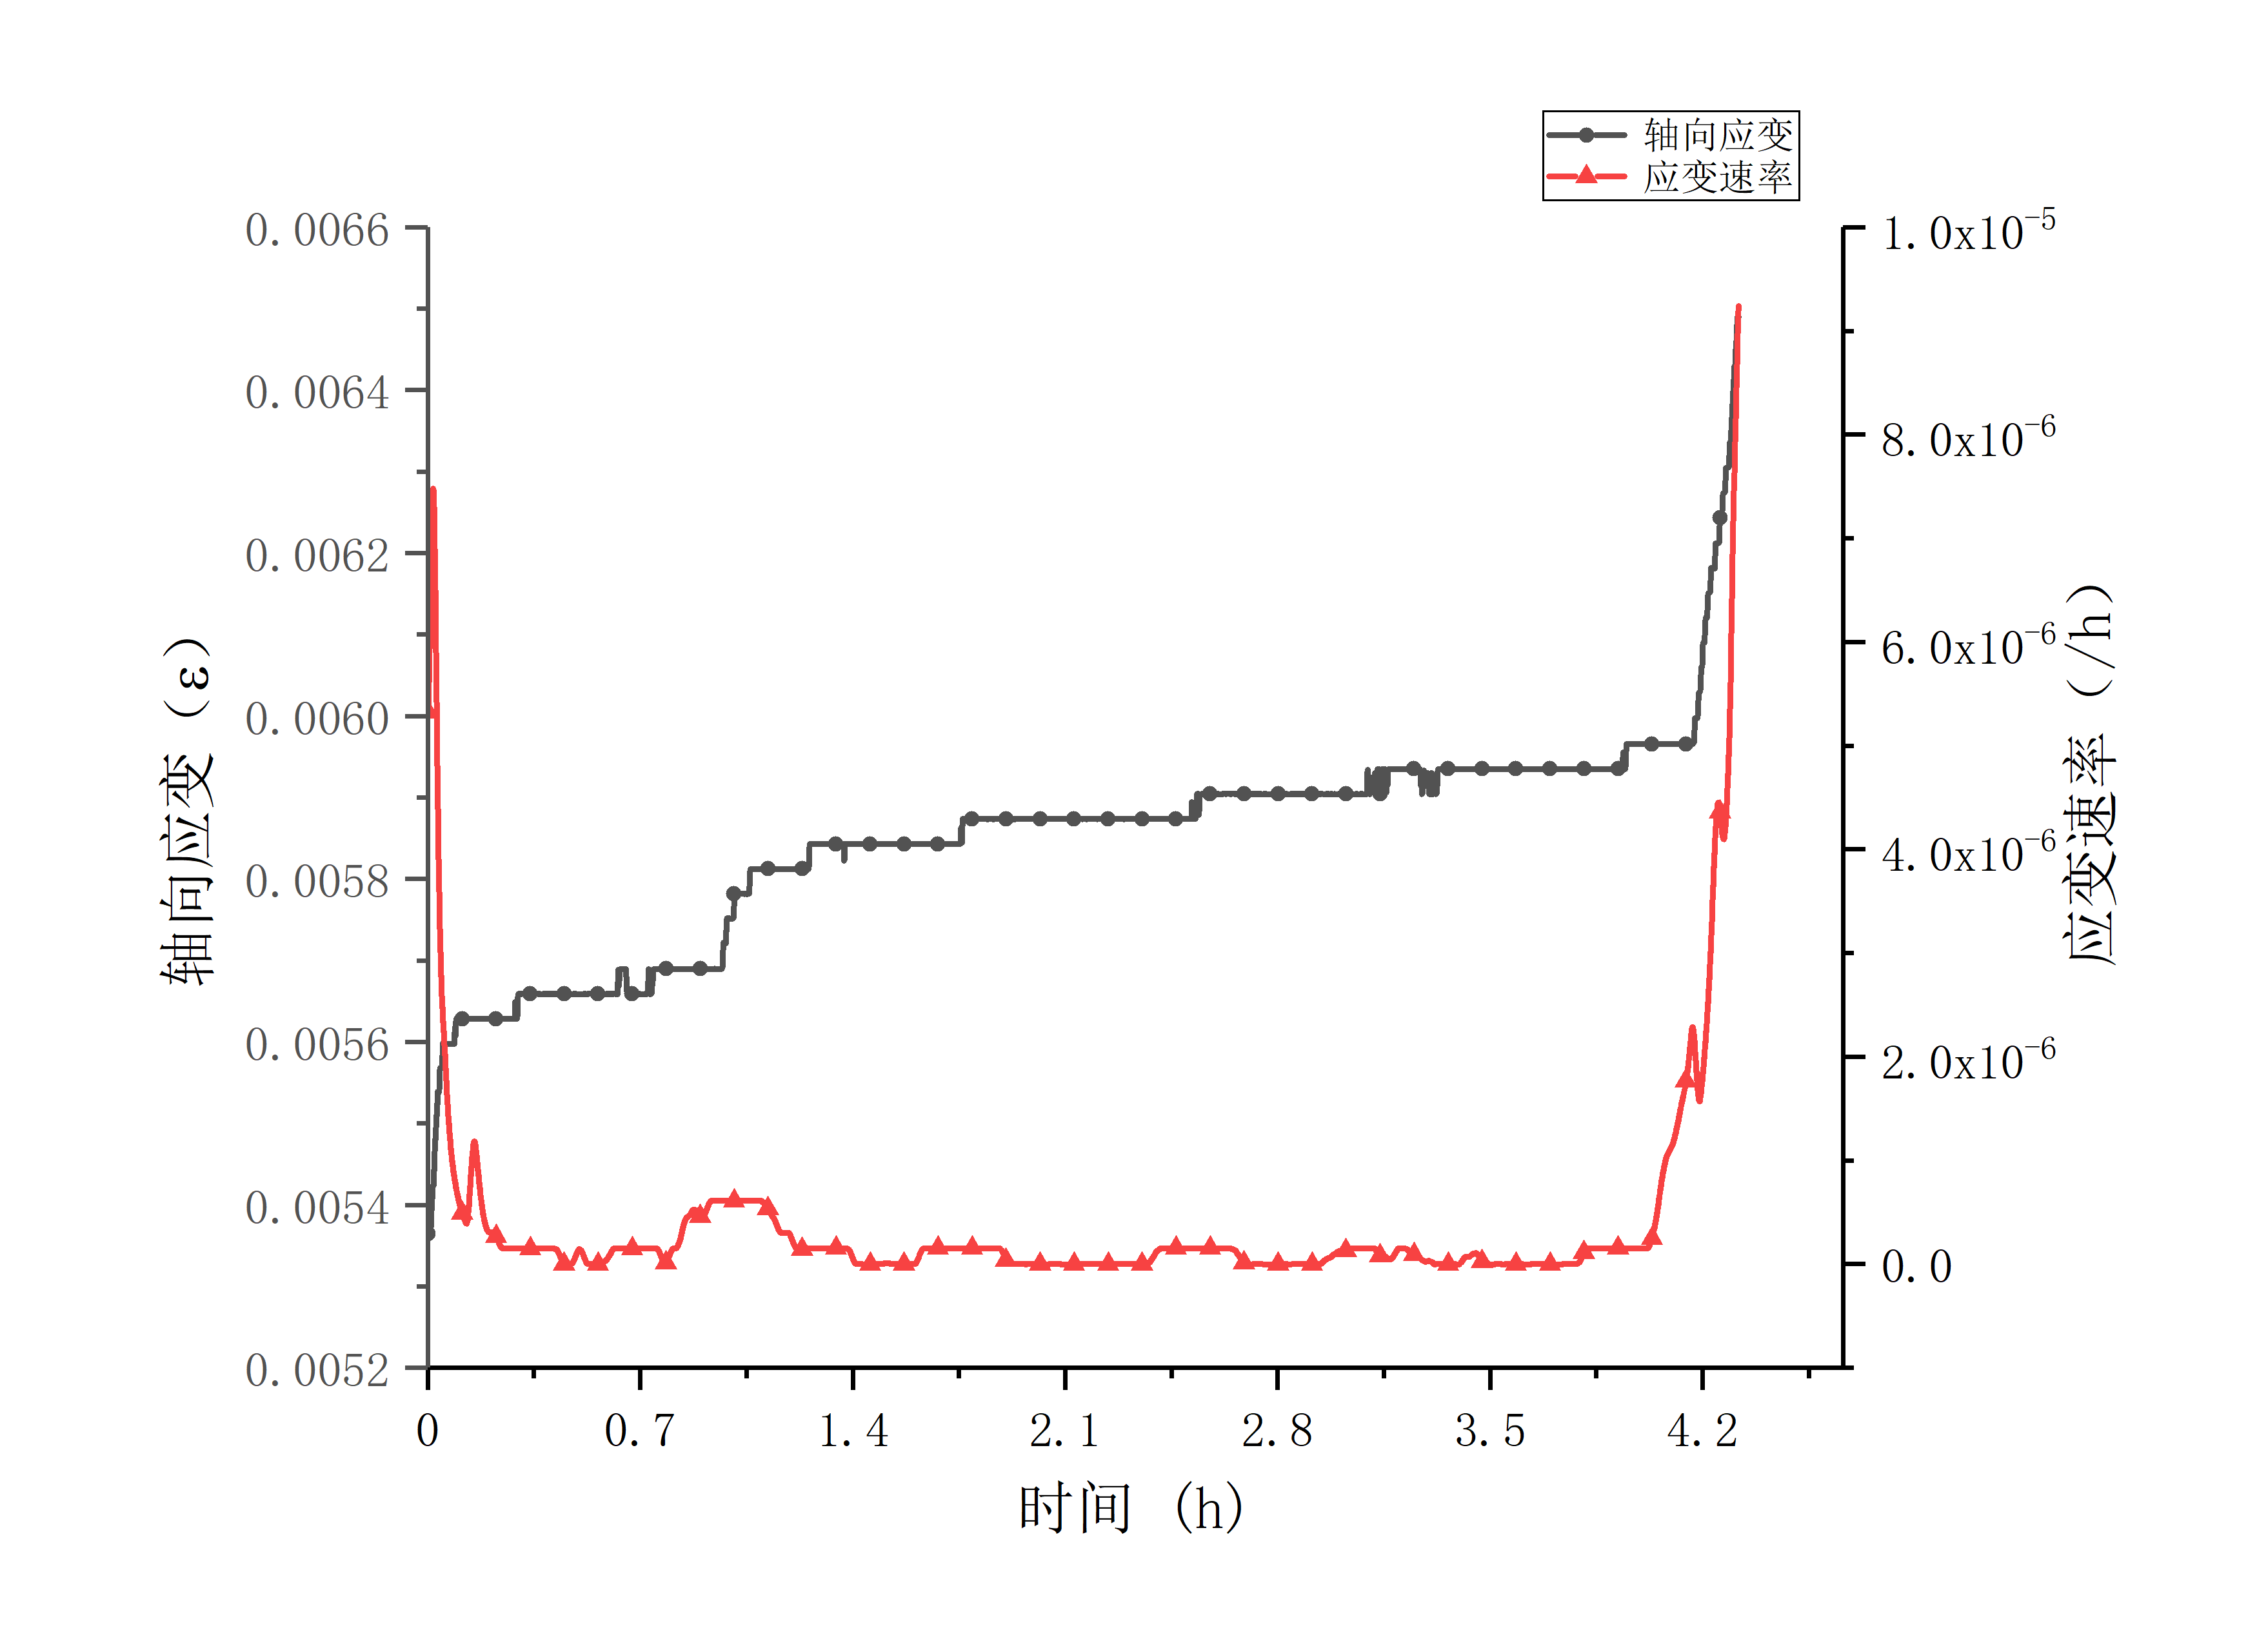
\includegraphics[width=1.2\textwidth]{img/chap2/D-01-v.png}
        \end{minipage}
    }
    \subfigure[D-02]
    {
        \begin{minipage}{7cm}
            \centering
            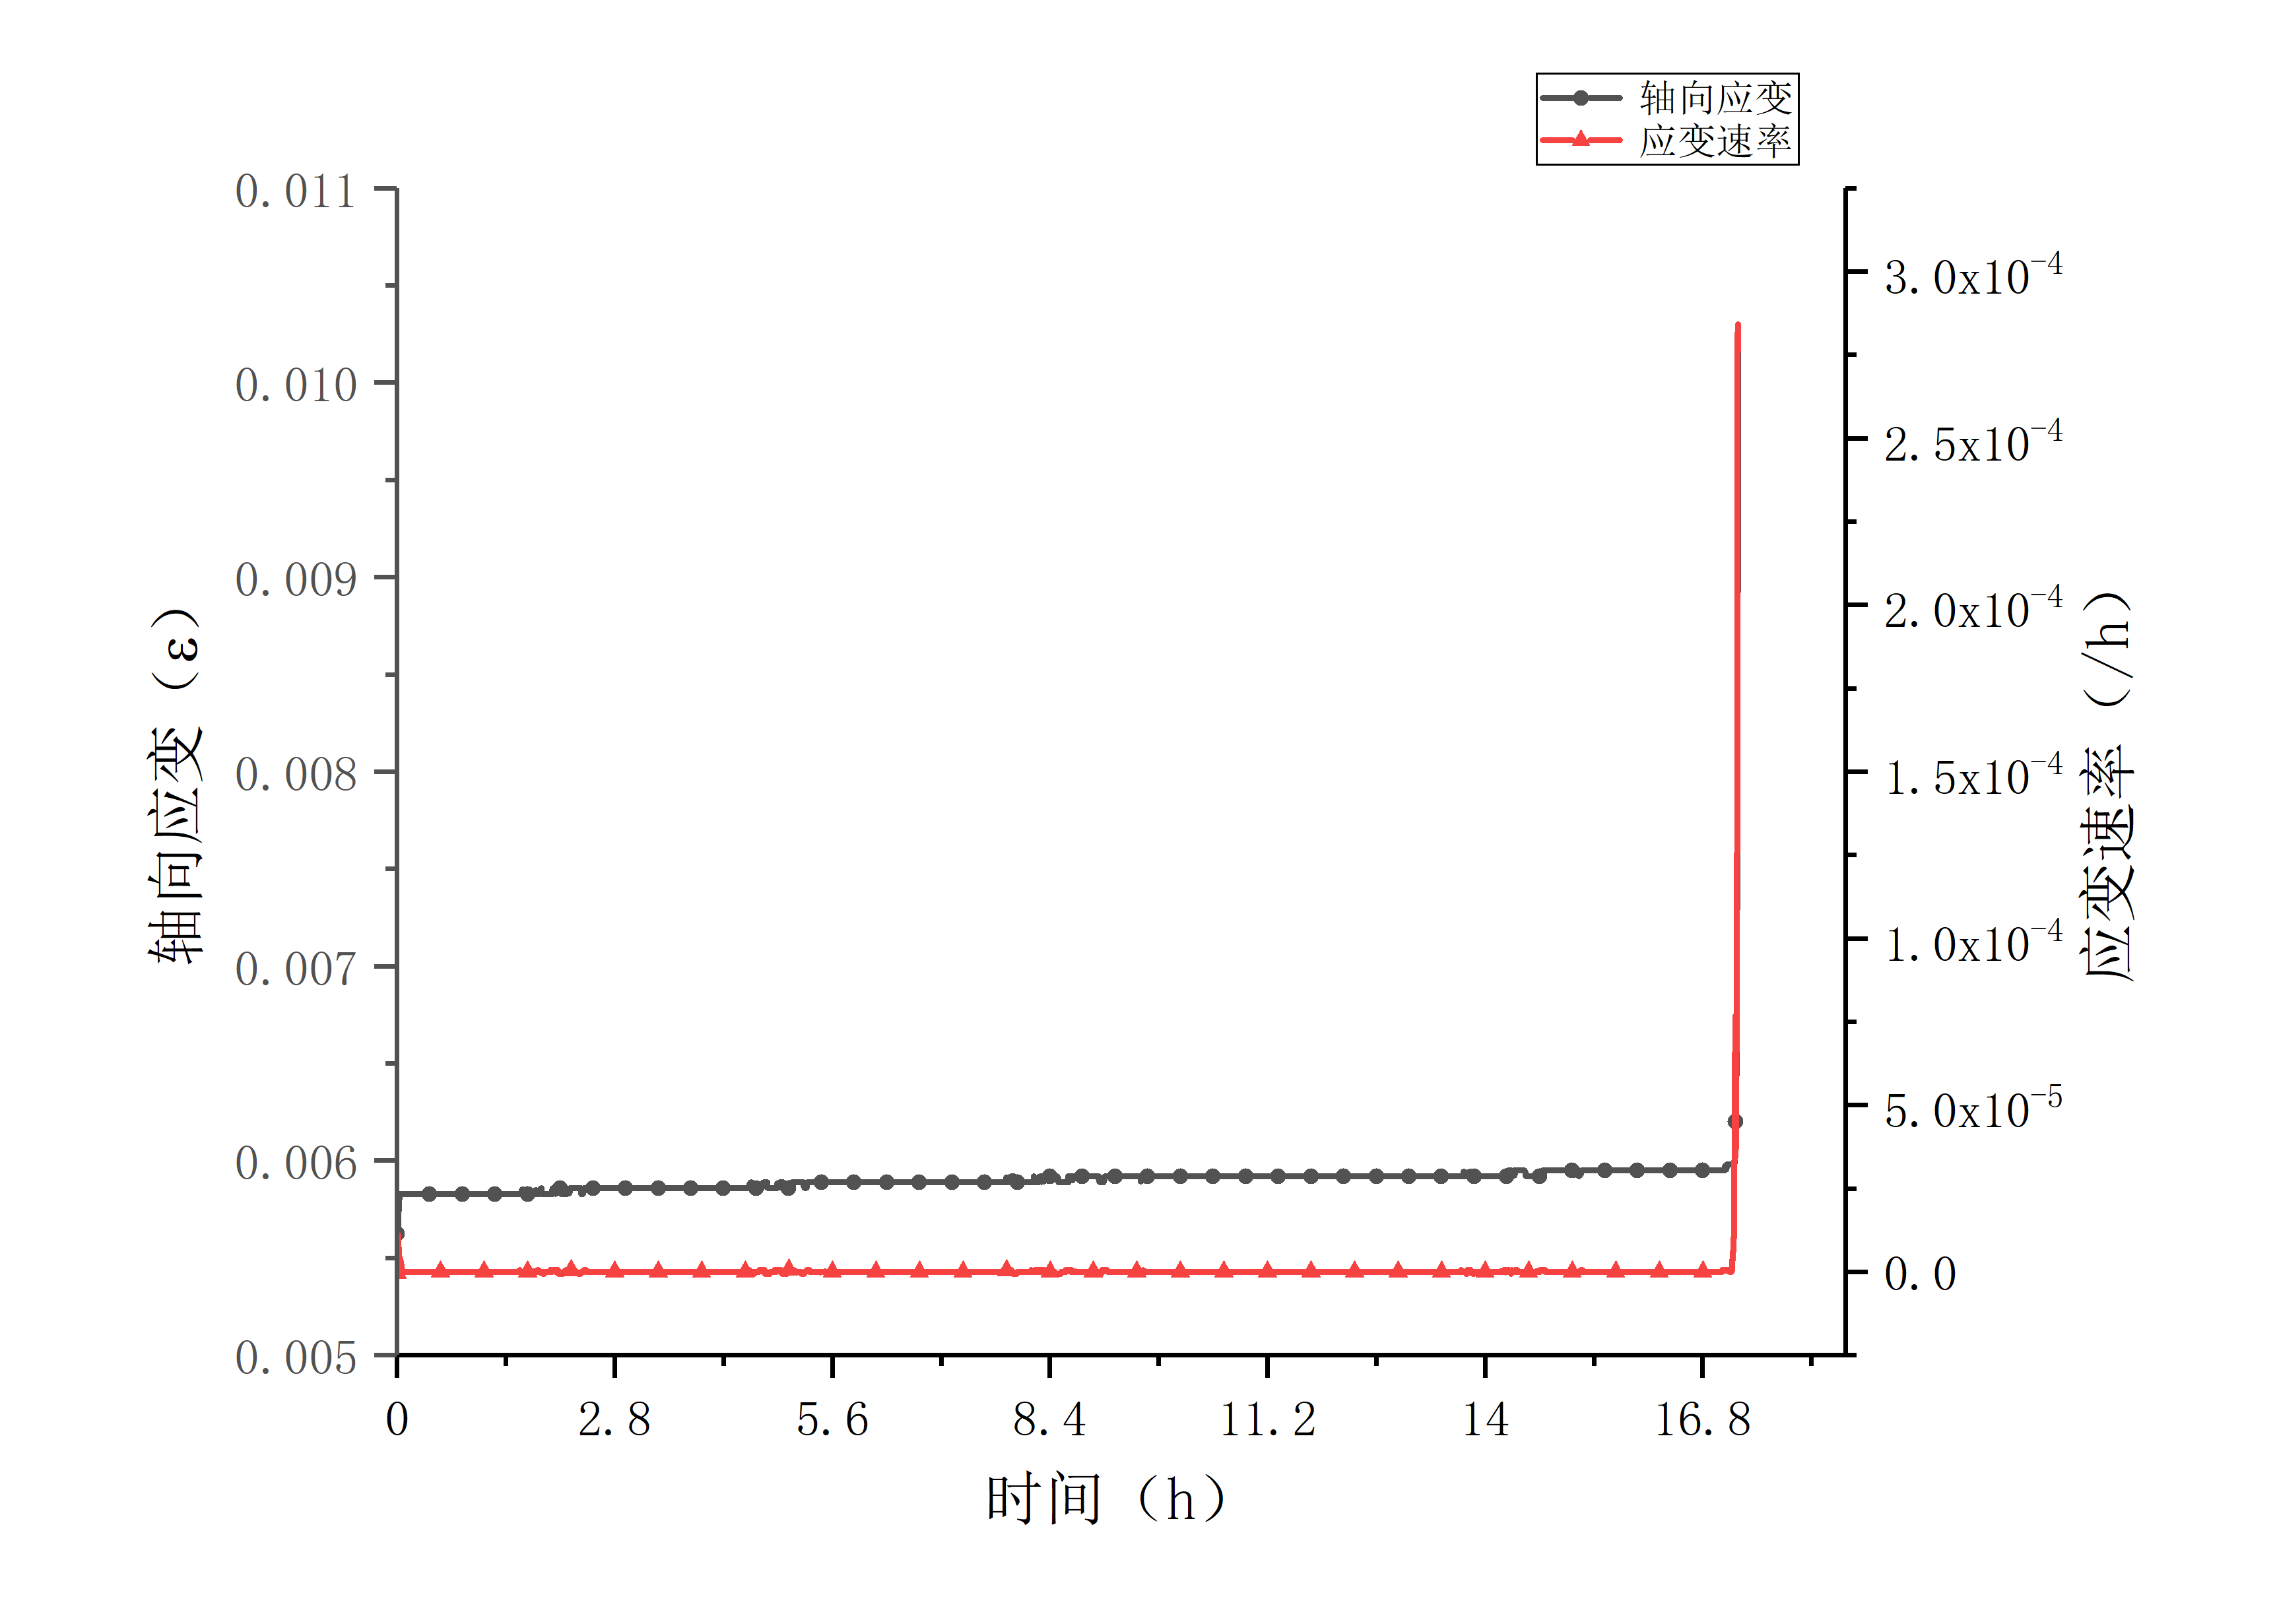
\includegraphics[width=1.2\textwidth]{img/chap2/D-02-v.png}
        \end{minipage}
    }
	
    \centering
    \subfigure[D-03]
    {
        \begin{minipage}{7cm}
            \centering
            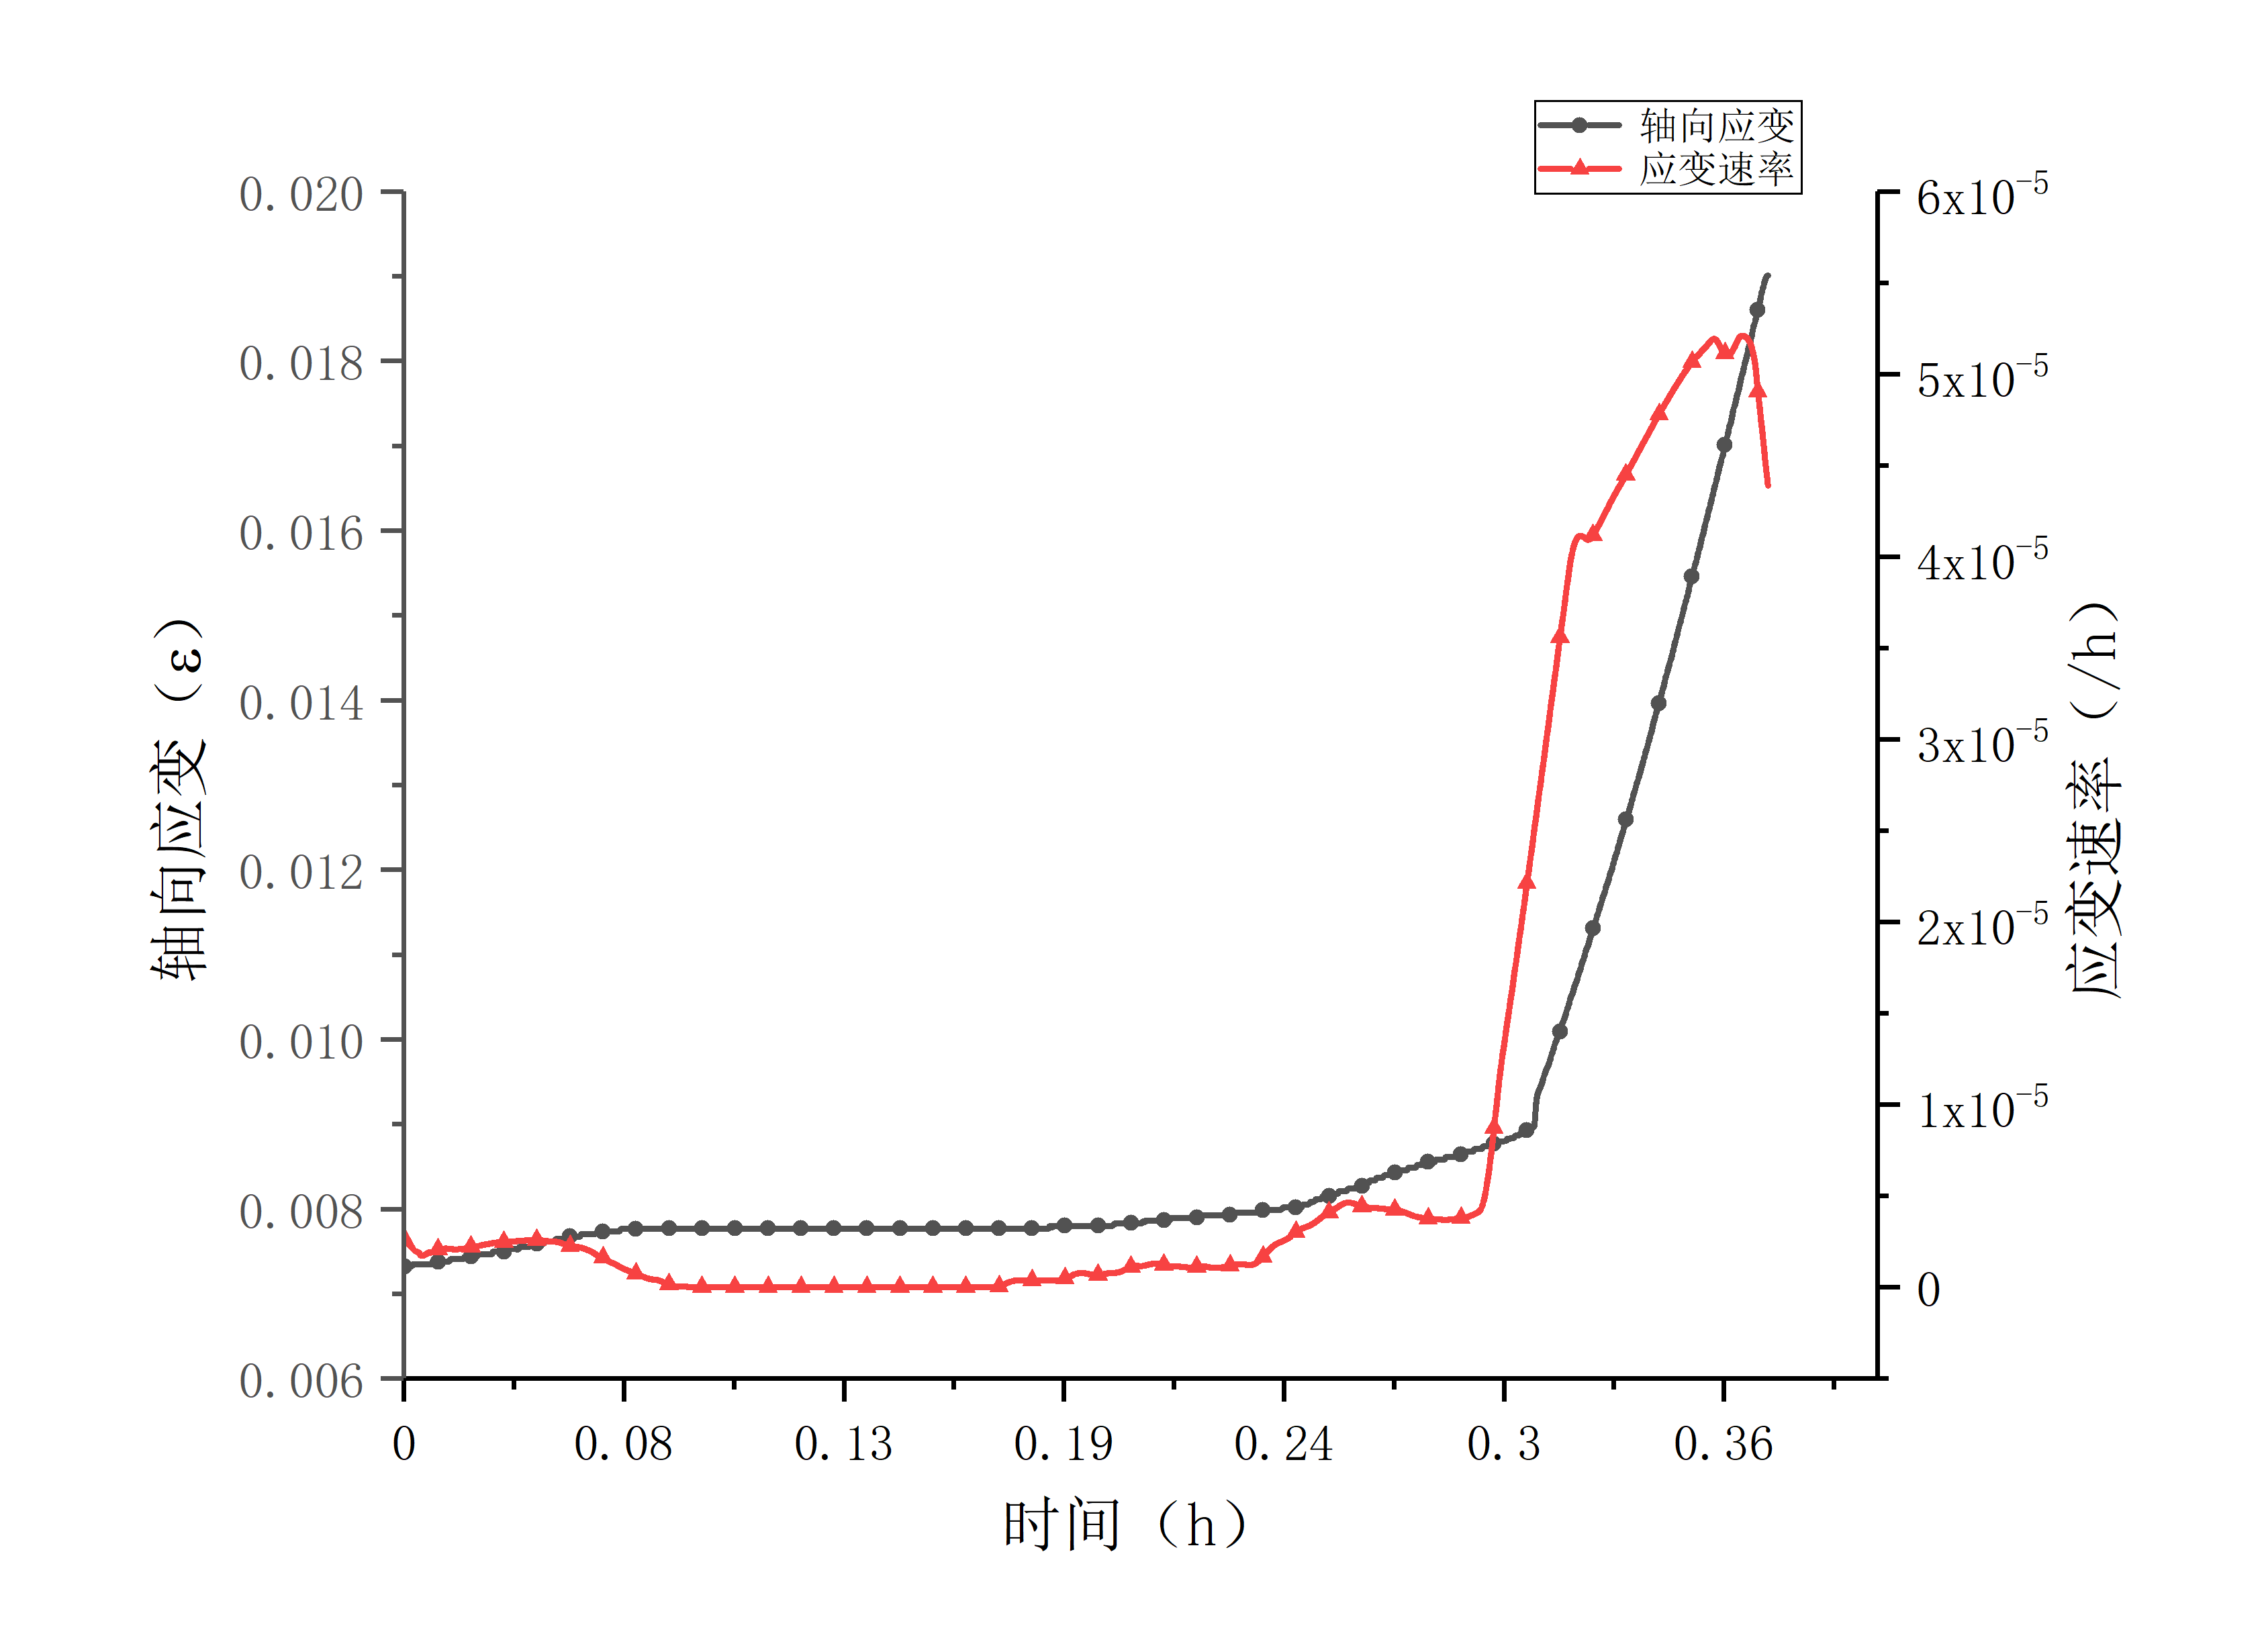
\includegraphics[width=1.2\textwidth]{img/chap2/D-03-v.png}
        \end{minipage}
    }
    \centering
    \caption{加速流变阶段曲线}
    \label{fig:2-13}
\end{figure}

在表示D-03试验的图(c)中,试样仅经历了一小段时间的稳定蠕变,在最后一级加载开始\SI{0.3}{h}后试样就进入了加速蠕变阶段,结合该组试验的数据,研究表明了D-03试样在最后一级加载刚开始时试样就发生了破坏,可以认为在第一阶段的加载过程中岩样已经积累大量损伤,在第二级应力施加仅仅不到20分钟就发生破裂,这主要是因为预期施加的应力过大,超过了泥岩试样的长期强度,导致了试样快速破裂,在此不作为流变破坏探讨。

除D-03以外的两组试验,根据图\ref{fig:2-13}中的(a)、(b)可以发现,试样在最后一级应力加载过程中均经历了衰减蠕变,稳定蠕变和加速蠕变三阶段。泥岩试样流变速率在衰减蠕变阶段逐渐减小,进入稳定蠕变阶段趋于某一较低值。在加速流变阶段,试样的轴向应变突然迅速增加,与此同时,应变速率在同一点处也由稳定的较低值迅速增大,根据记载的数据,轴向应力也迅速减小,从宏观上可以观察到,此时试样出现大量裂缝,试样破坏。
D-01的流变曲线较为光滑,表现为渐进性加速破坏,属韧性破坏,其流变破坏可预见性较高;D-02的流变曲线呈突变性增长,突变起点对应流变速率变化的尖点,反映硬脆性岩石流变破裂特点,其流变破坏可预见性较低。

加速流变阶段尽管只占据流变试验较短的时间,但该阶段流变量却占据流变变形量的主要部分。最后一级应力下试样在不同蠕变阶段历时及流变变形量如表\ref{tab:最后一级应力下试样流变参数}所示。
\begin{table}[H]
\centering
\begin{tabular}{ccccc}%四个c代表有四列且内容居中
\toprule%第一道横线
\multirow{2}{*}{试样编号}&\multicolumn{2}{c}{\textbf{\underline{衰减、稳定蠕变阶段}}}& \multicolumn{2}{c}{\textbf{\underline{加速蠕变阶段}}}  \\
&时间/h & 应变/$\mu\varepsilon$ & 时间/h & 应变/$\mu\varepsilon$ \\
\midrule%第二道横线 
D-01  &4.8&550& 0.4 & 560 \\%Data1跨两行,自动表格宽度
\midrule%第三道横线 
D-02&16.86&330&0.4&4250 \\
\midrule
D-03&0.3&1580& 0.006&10100 \\
\bottomrule%第四道横线
\end{tabular}
\caption{最后一级应力下试样流变参数}
\label{tab:最后一级应力下试样流变参数}
\end{table}



\section{流变对应力—应变曲线的影响}

岩石试样单轴流变作用对应力-应变曲线的影响如图\ref{fig:2-14}所示,与x轴近似平行的曲线部分即代表流变变形。
在应力等级较低时,岩石流变变形量较小,随着应力等级提高,
流变变形显著,这与流变变形与时间的规律完全吻合。与单轴压缩试验下应
力一应变曲线相比,流变作用下的应力一应变曲线也反映了孔隙裂隙压密阶段、弹性
变形阶段、微破裂发展阶段这三个阶段,不过在本次试验中,只有C-03试样最终发生破坏,因此峰后破坏阶段只在图\ref{fig:2-14}(c)中有所体现。图\ref{fig:2-15}所示为三轴流变试验应力-应变曲线图,三组试验曲线都出现了峰后破坏阶段,说明三轴流变试验中试样最后全部破坏了。图中与x轴平行的曲线代表了稳定蠕变阶段,而从图中也可也看出曲线的阶梯状增长趋势,这代表了试验中的分级加载过程。

根据表\ref{tab:泥岩单、三轴流变试验结果}与表\ref{tab:泥岩单、三轴试验结果}相比较,单轴流变试验弹性模量为11.171GPa,三轴流变试验弹性模量为12.580GPa,变作用下试样的弹性模量总体上小于瞬时弹性模量,
而在单轴流变试验中,虽然仅有C-03试样发生破坏,不过根据应力-应变曲线图结果数据可以判断,在流变作用下,破坏时变形量大于瞬时峰值应变,蠕变破坏强度小于瞬时破坏强度。

\begin{table}[ht!]\small
    \begin{tabular}{p{3cm}<{\centering} p{3cm}<{\centering} p{3cm}<{\centering} p{3cm}<{\centering}}
        \toprule
        试样编号  & 峰值强度/MPa  &  破坏时应变   & 弹性模量/GPa\\
        \midrule
        C-01        & 26.86  &   未破坏  &  12.048   \\ 
        C-02        & 24.96 &   未破坏  &  11.241   \\ 
        C-03        & 23.62  &   0.0032  &  10.947  \\ 
        C-04        & 22.10 &   未破坏  &  9.841   \\ 
        C-05        & 20.64  &   未破坏  &  11.742  \\
        \midrule
        D-01        & 74.01  &   0.0059  &  11.924    \\ 
        D-02        & 73.75 &   0.0058 &  13.145    \\ 
        D-03        & 89.14 &   0.0078  &  12.670 \\ 
        \bottomrule
    \end{tabular}
    \caption{泥岩单、三轴流变试验结果}
    \label{tab:泥岩单、三轴流变试验结果}
\end{table}

\begin{figure}[ht!]
    \centering
    \subfigure[D-01]
    {
        \begin{minipage}{7cm}
            \centering
            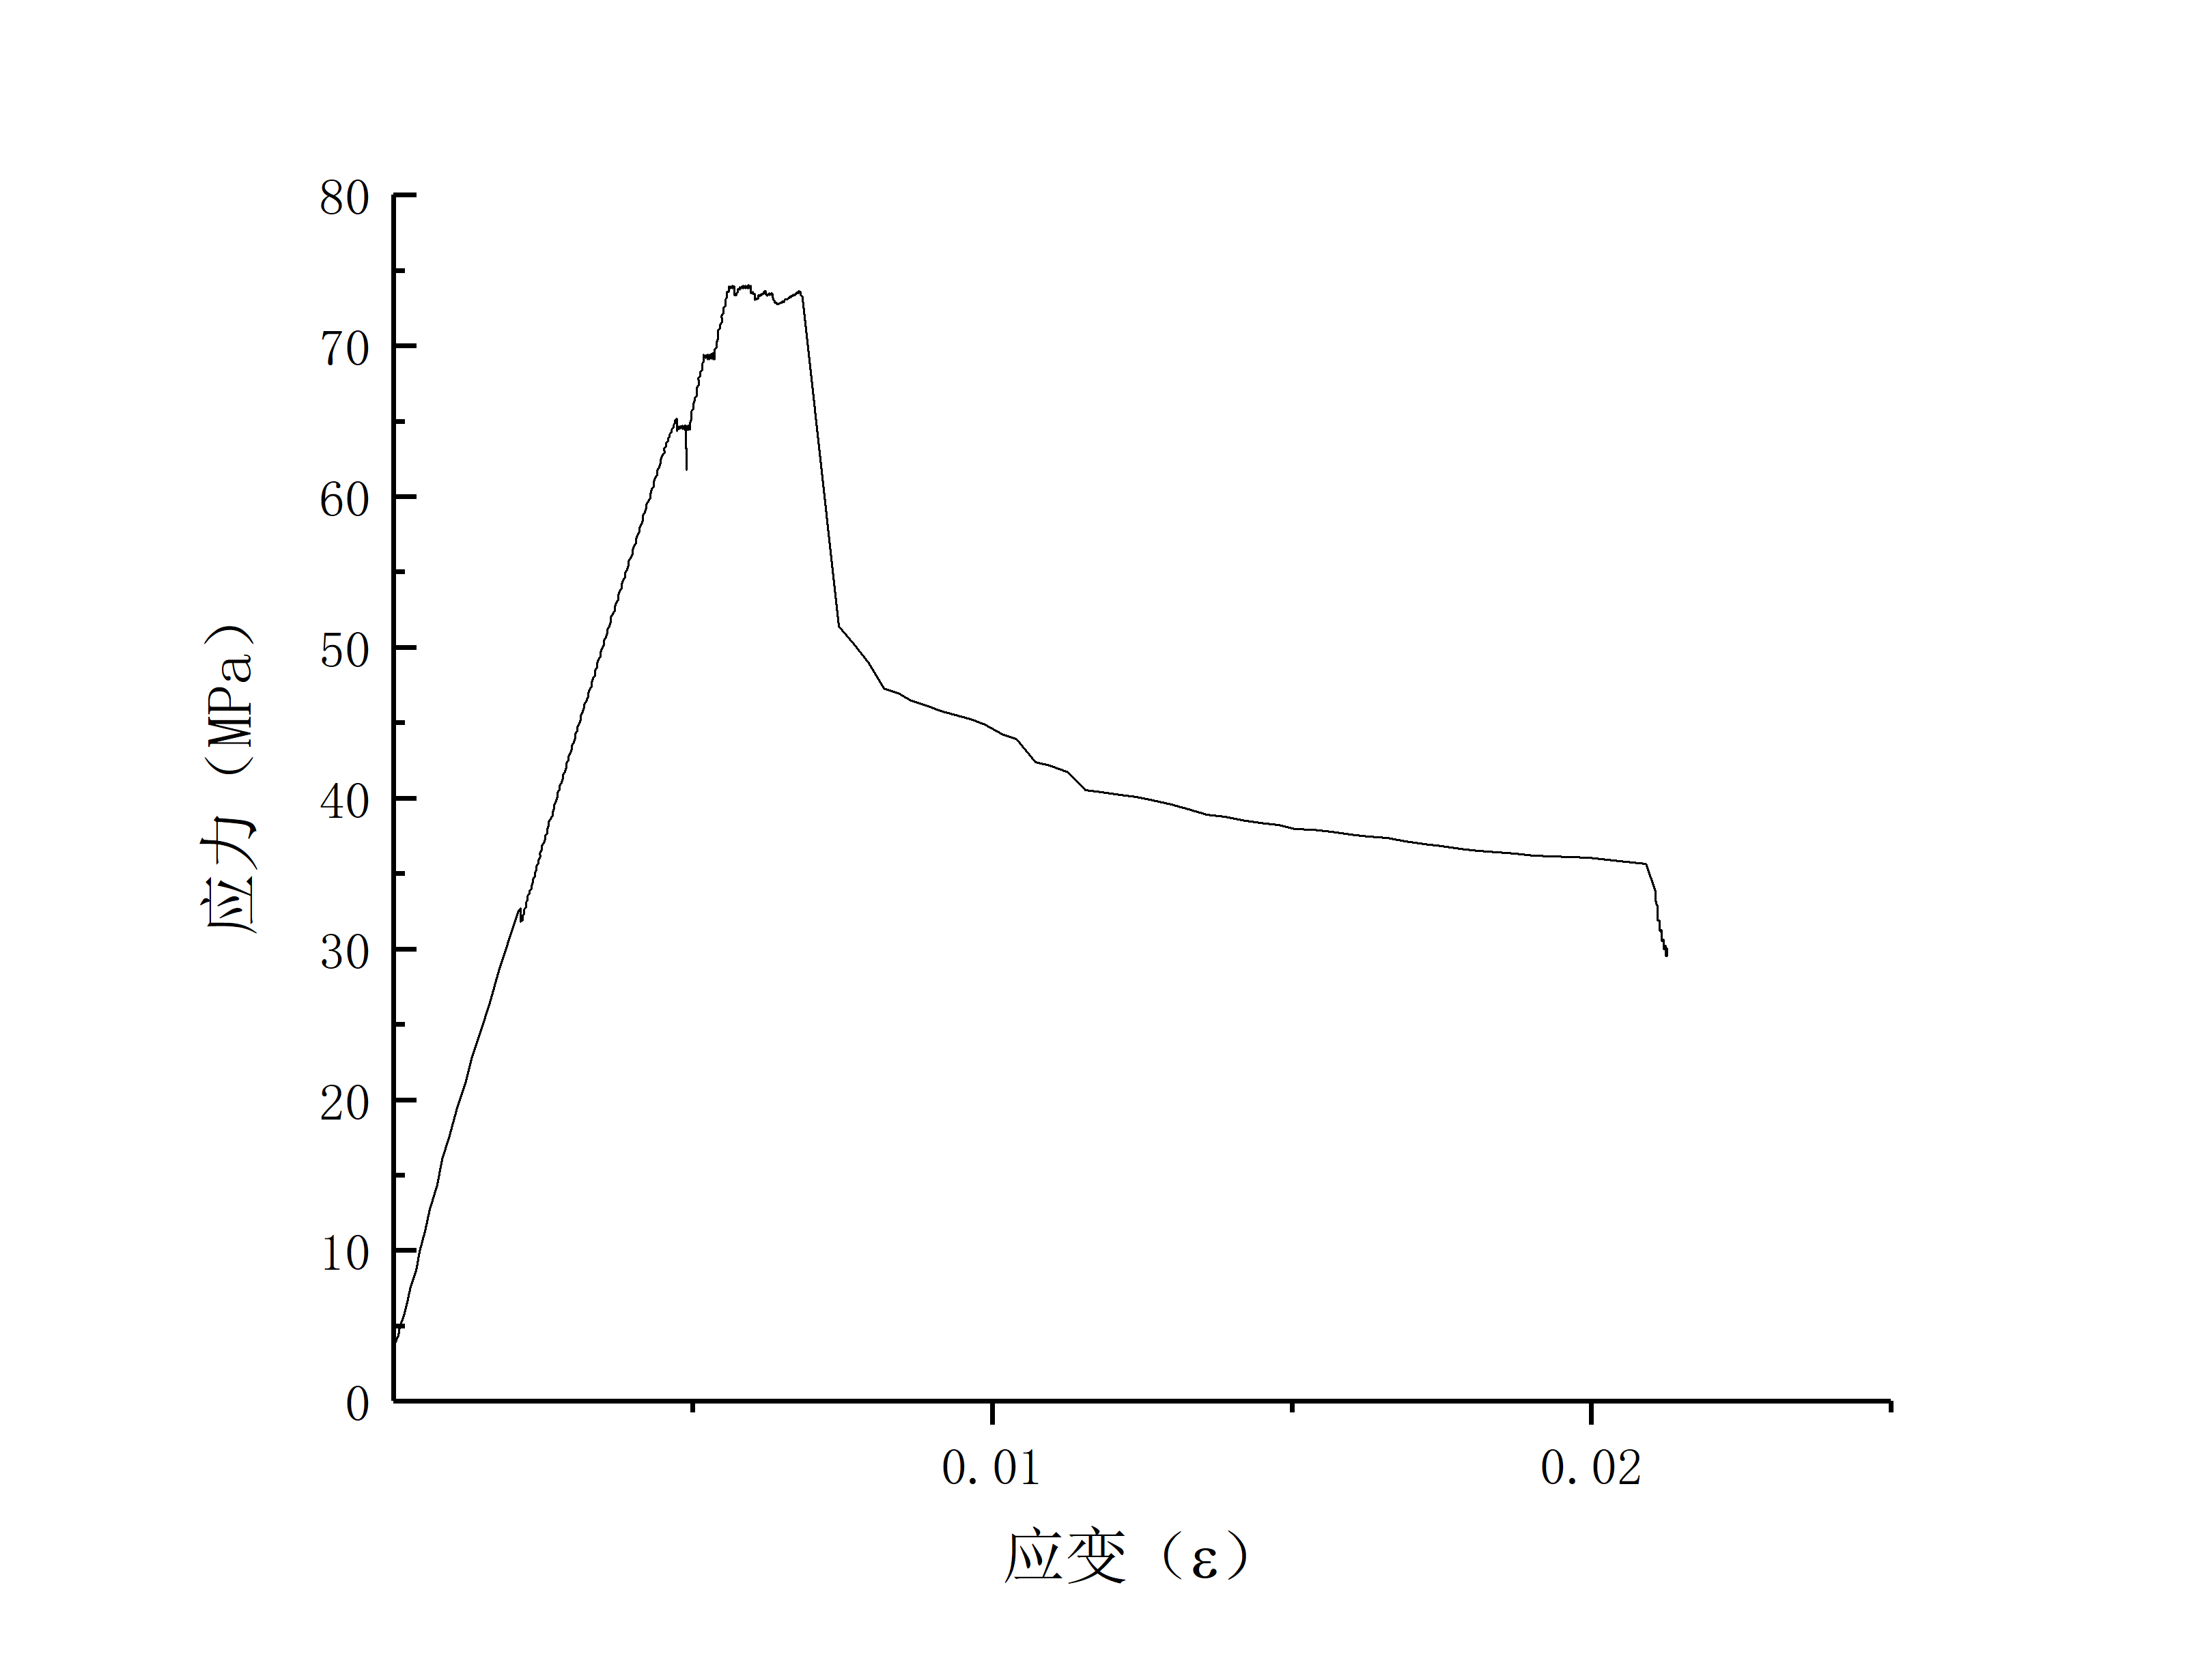
\includegraphics[width=1.1\textwidth]{img/chap2/stress-strain-D01.png}
        \end{minipage}
    }
    \subfigure[D-02]
    {
        \begin{minipage}{7cm}
            \centering
            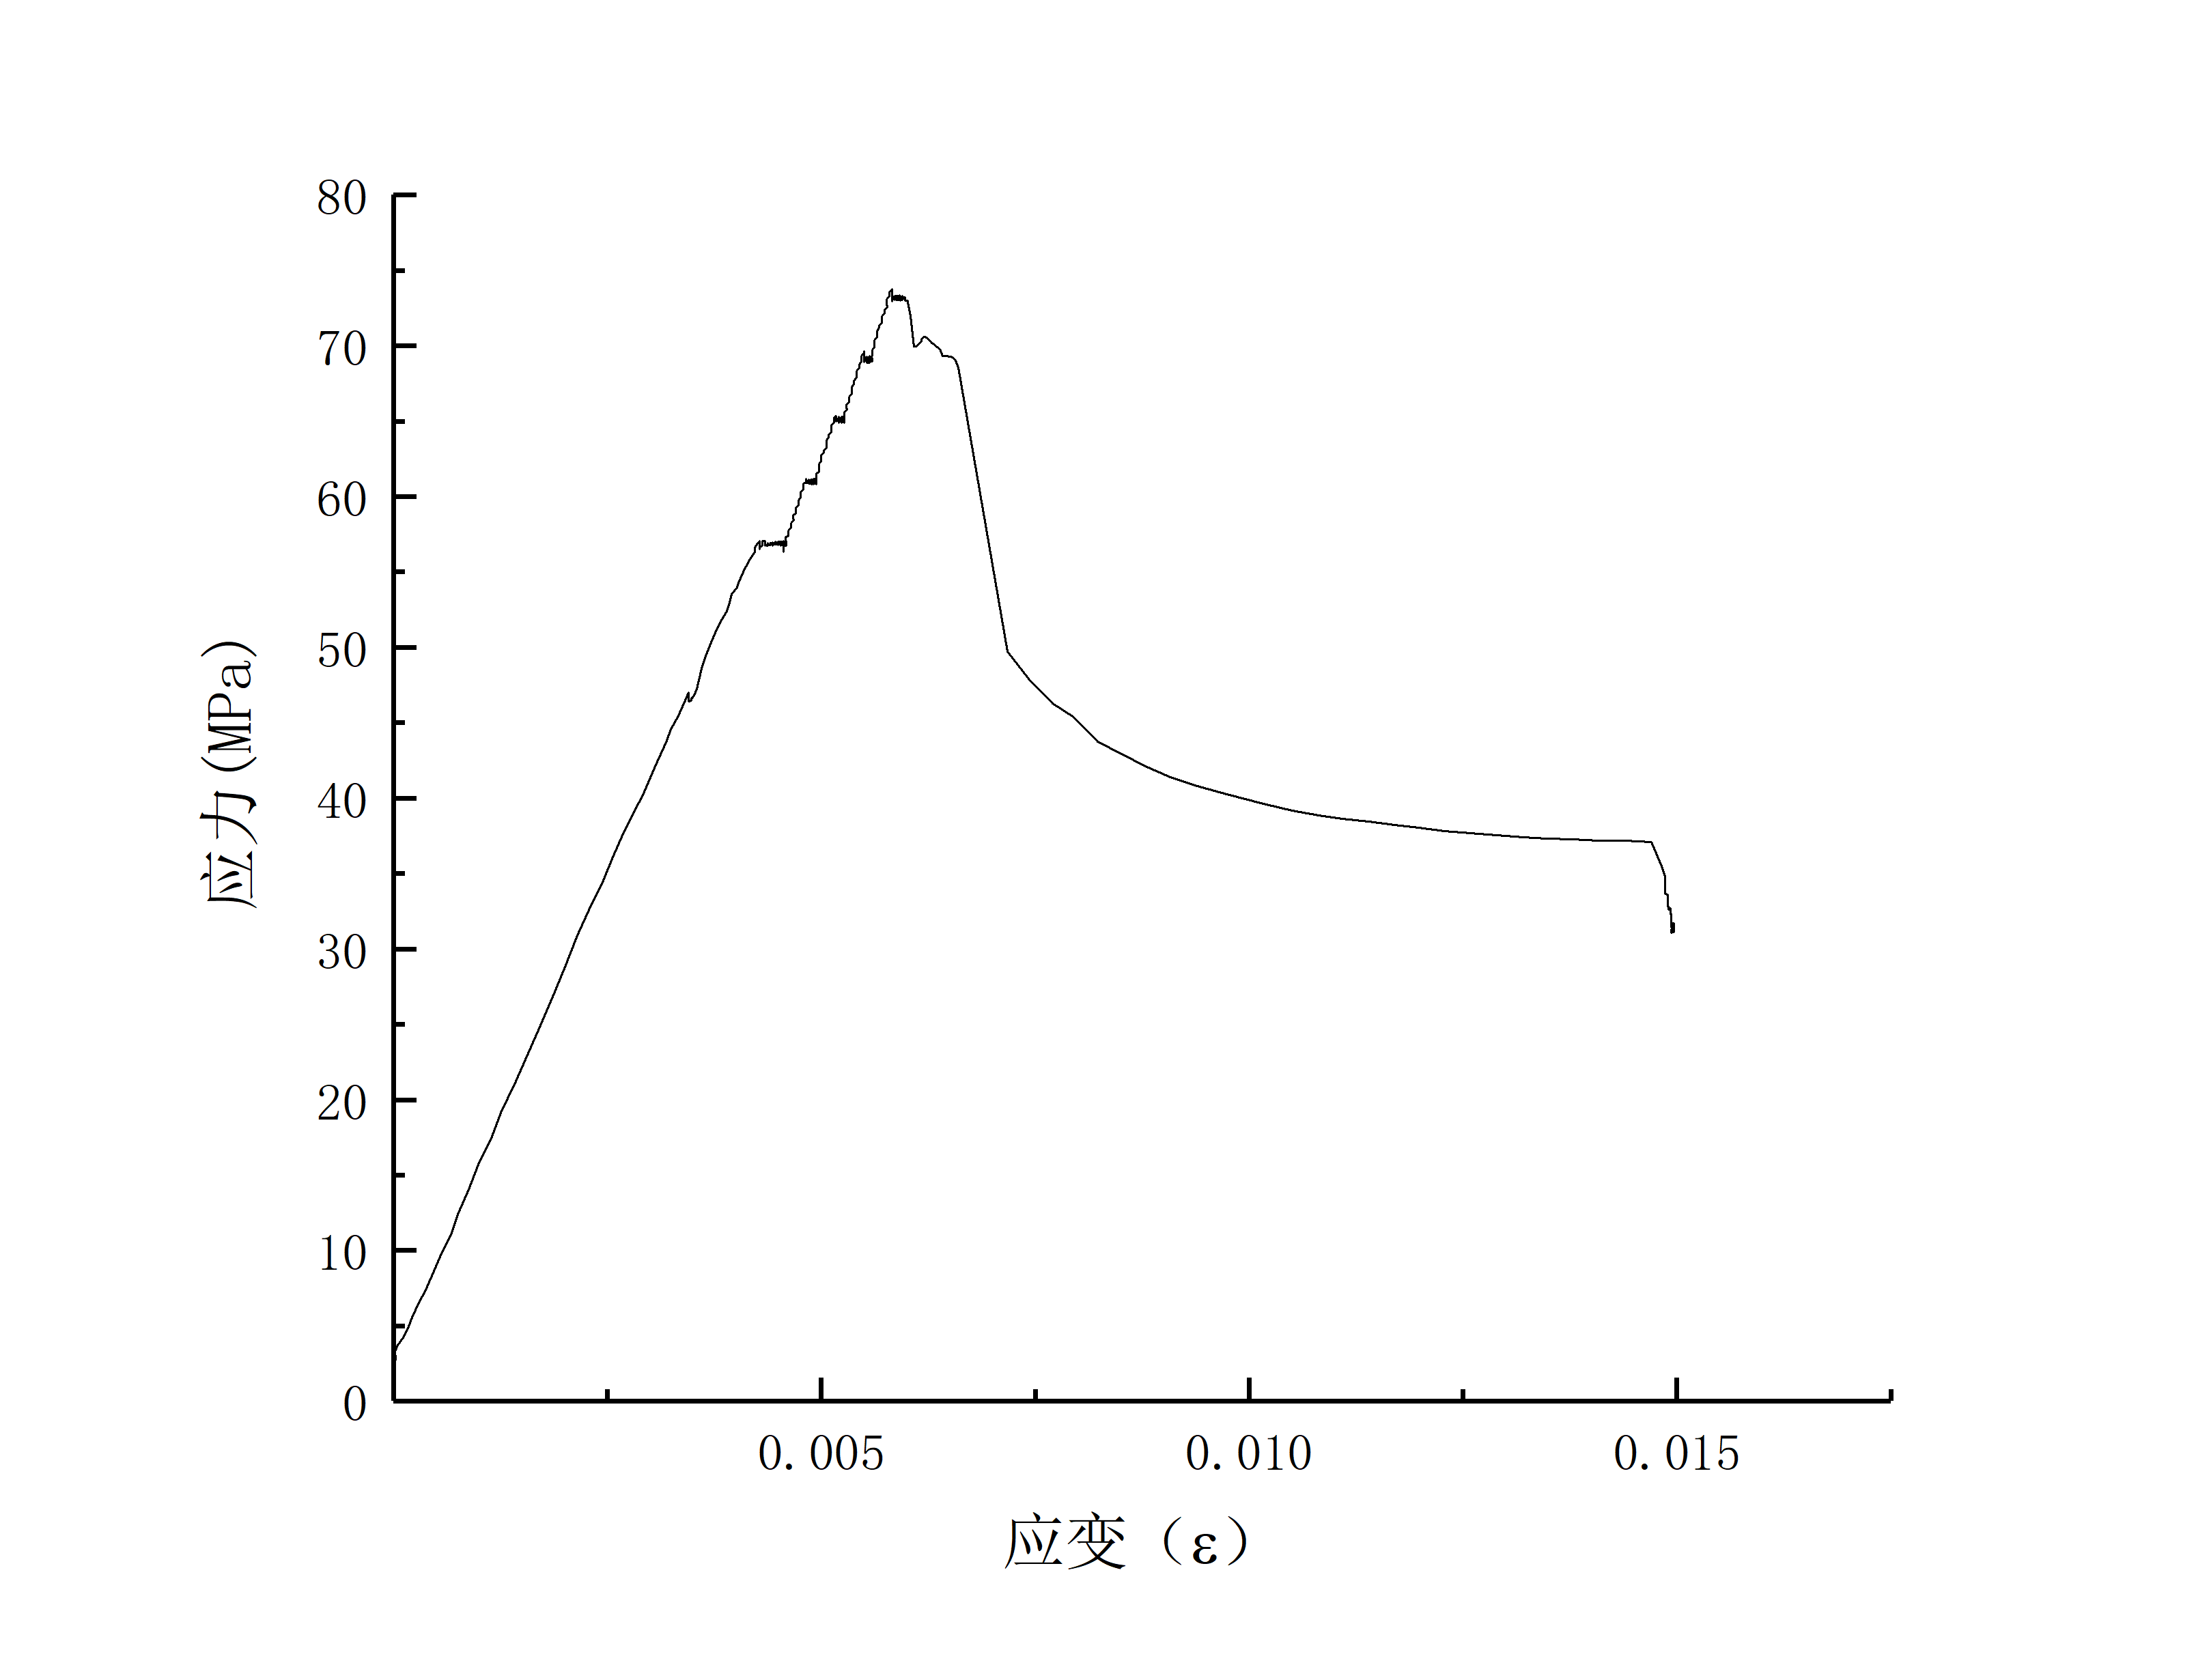
\includegraphics[width=1.1\textwidth]{img/chap2/stress-strain-D02.png}
        \end{minipage}
    }
	
    \subfigure[D-03]
    {
        \begin{minipage}{7cm}
            \centering
            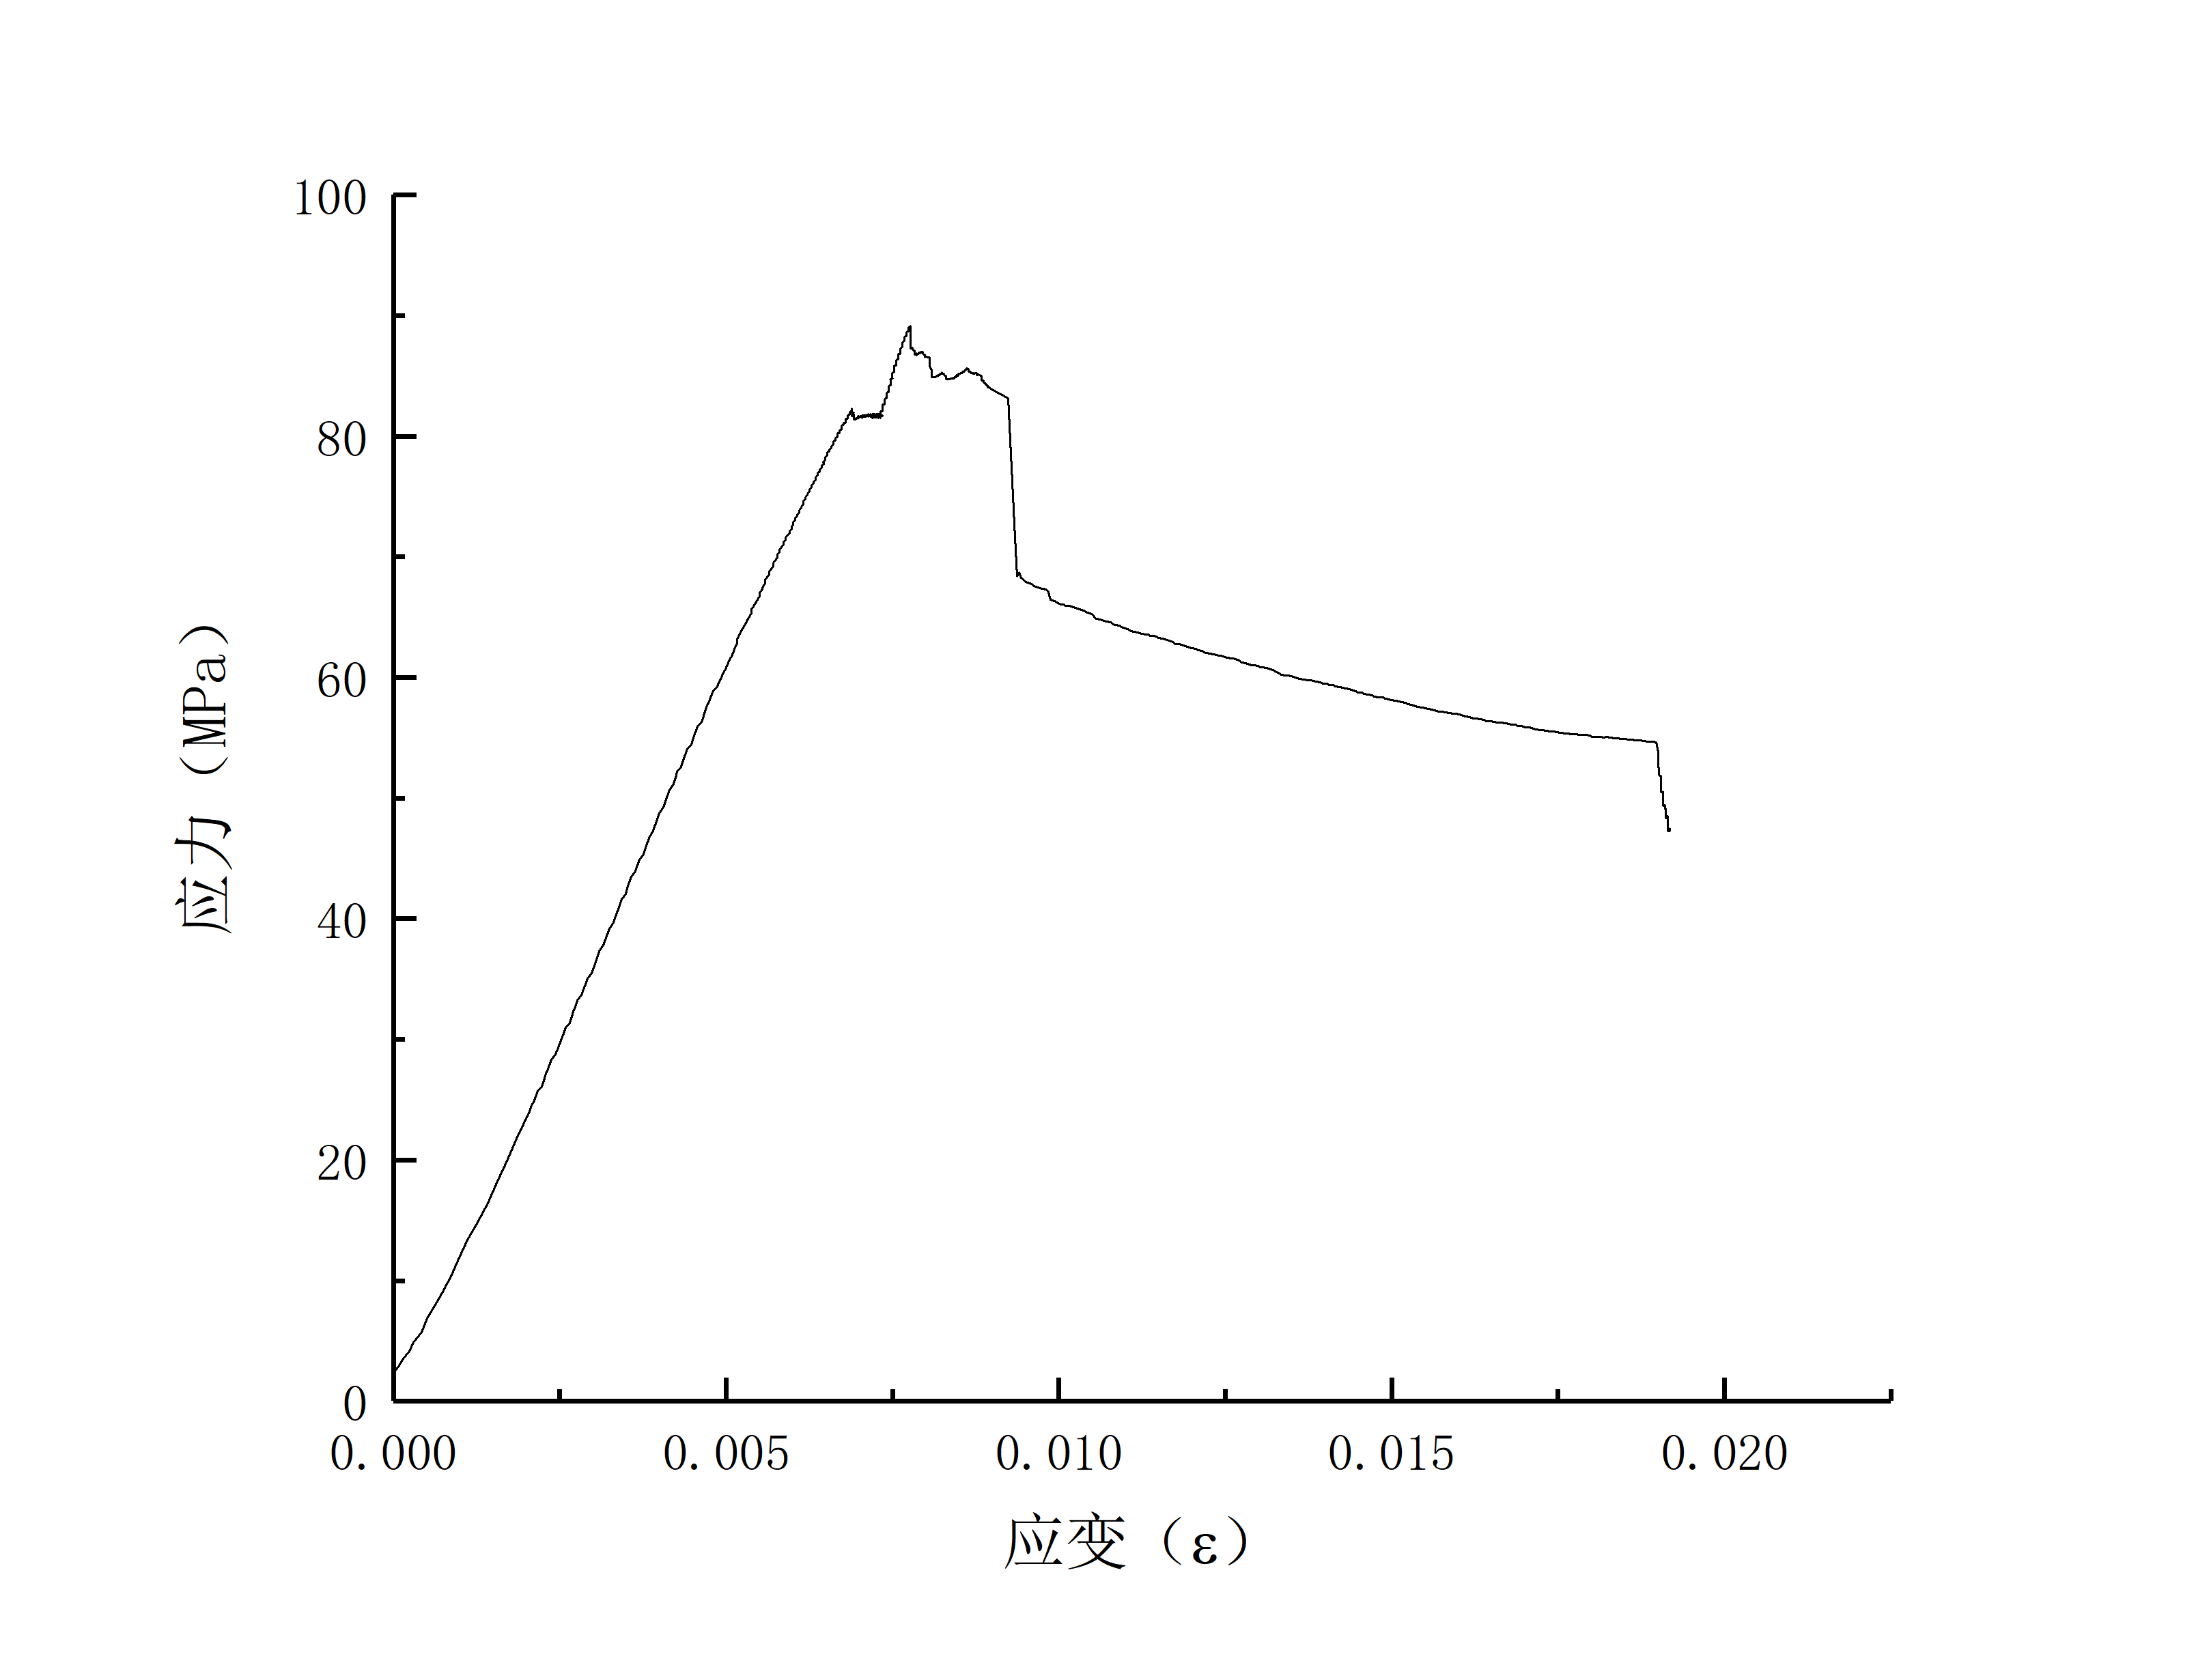
\includegraphics[width=1.1\textwidth]{img/chap2/stress-strain-D03.png}
        \end{minipage}
    }
    \centering
    \caption{三轴流变应力-应变曲线图}
    \label{fig:2-15}
\end{figure}



\begin{figure}[ht!]
    \centering
    \subfigure[C-01]
    {
        \begin{minipage}{7cm}
            \centering
            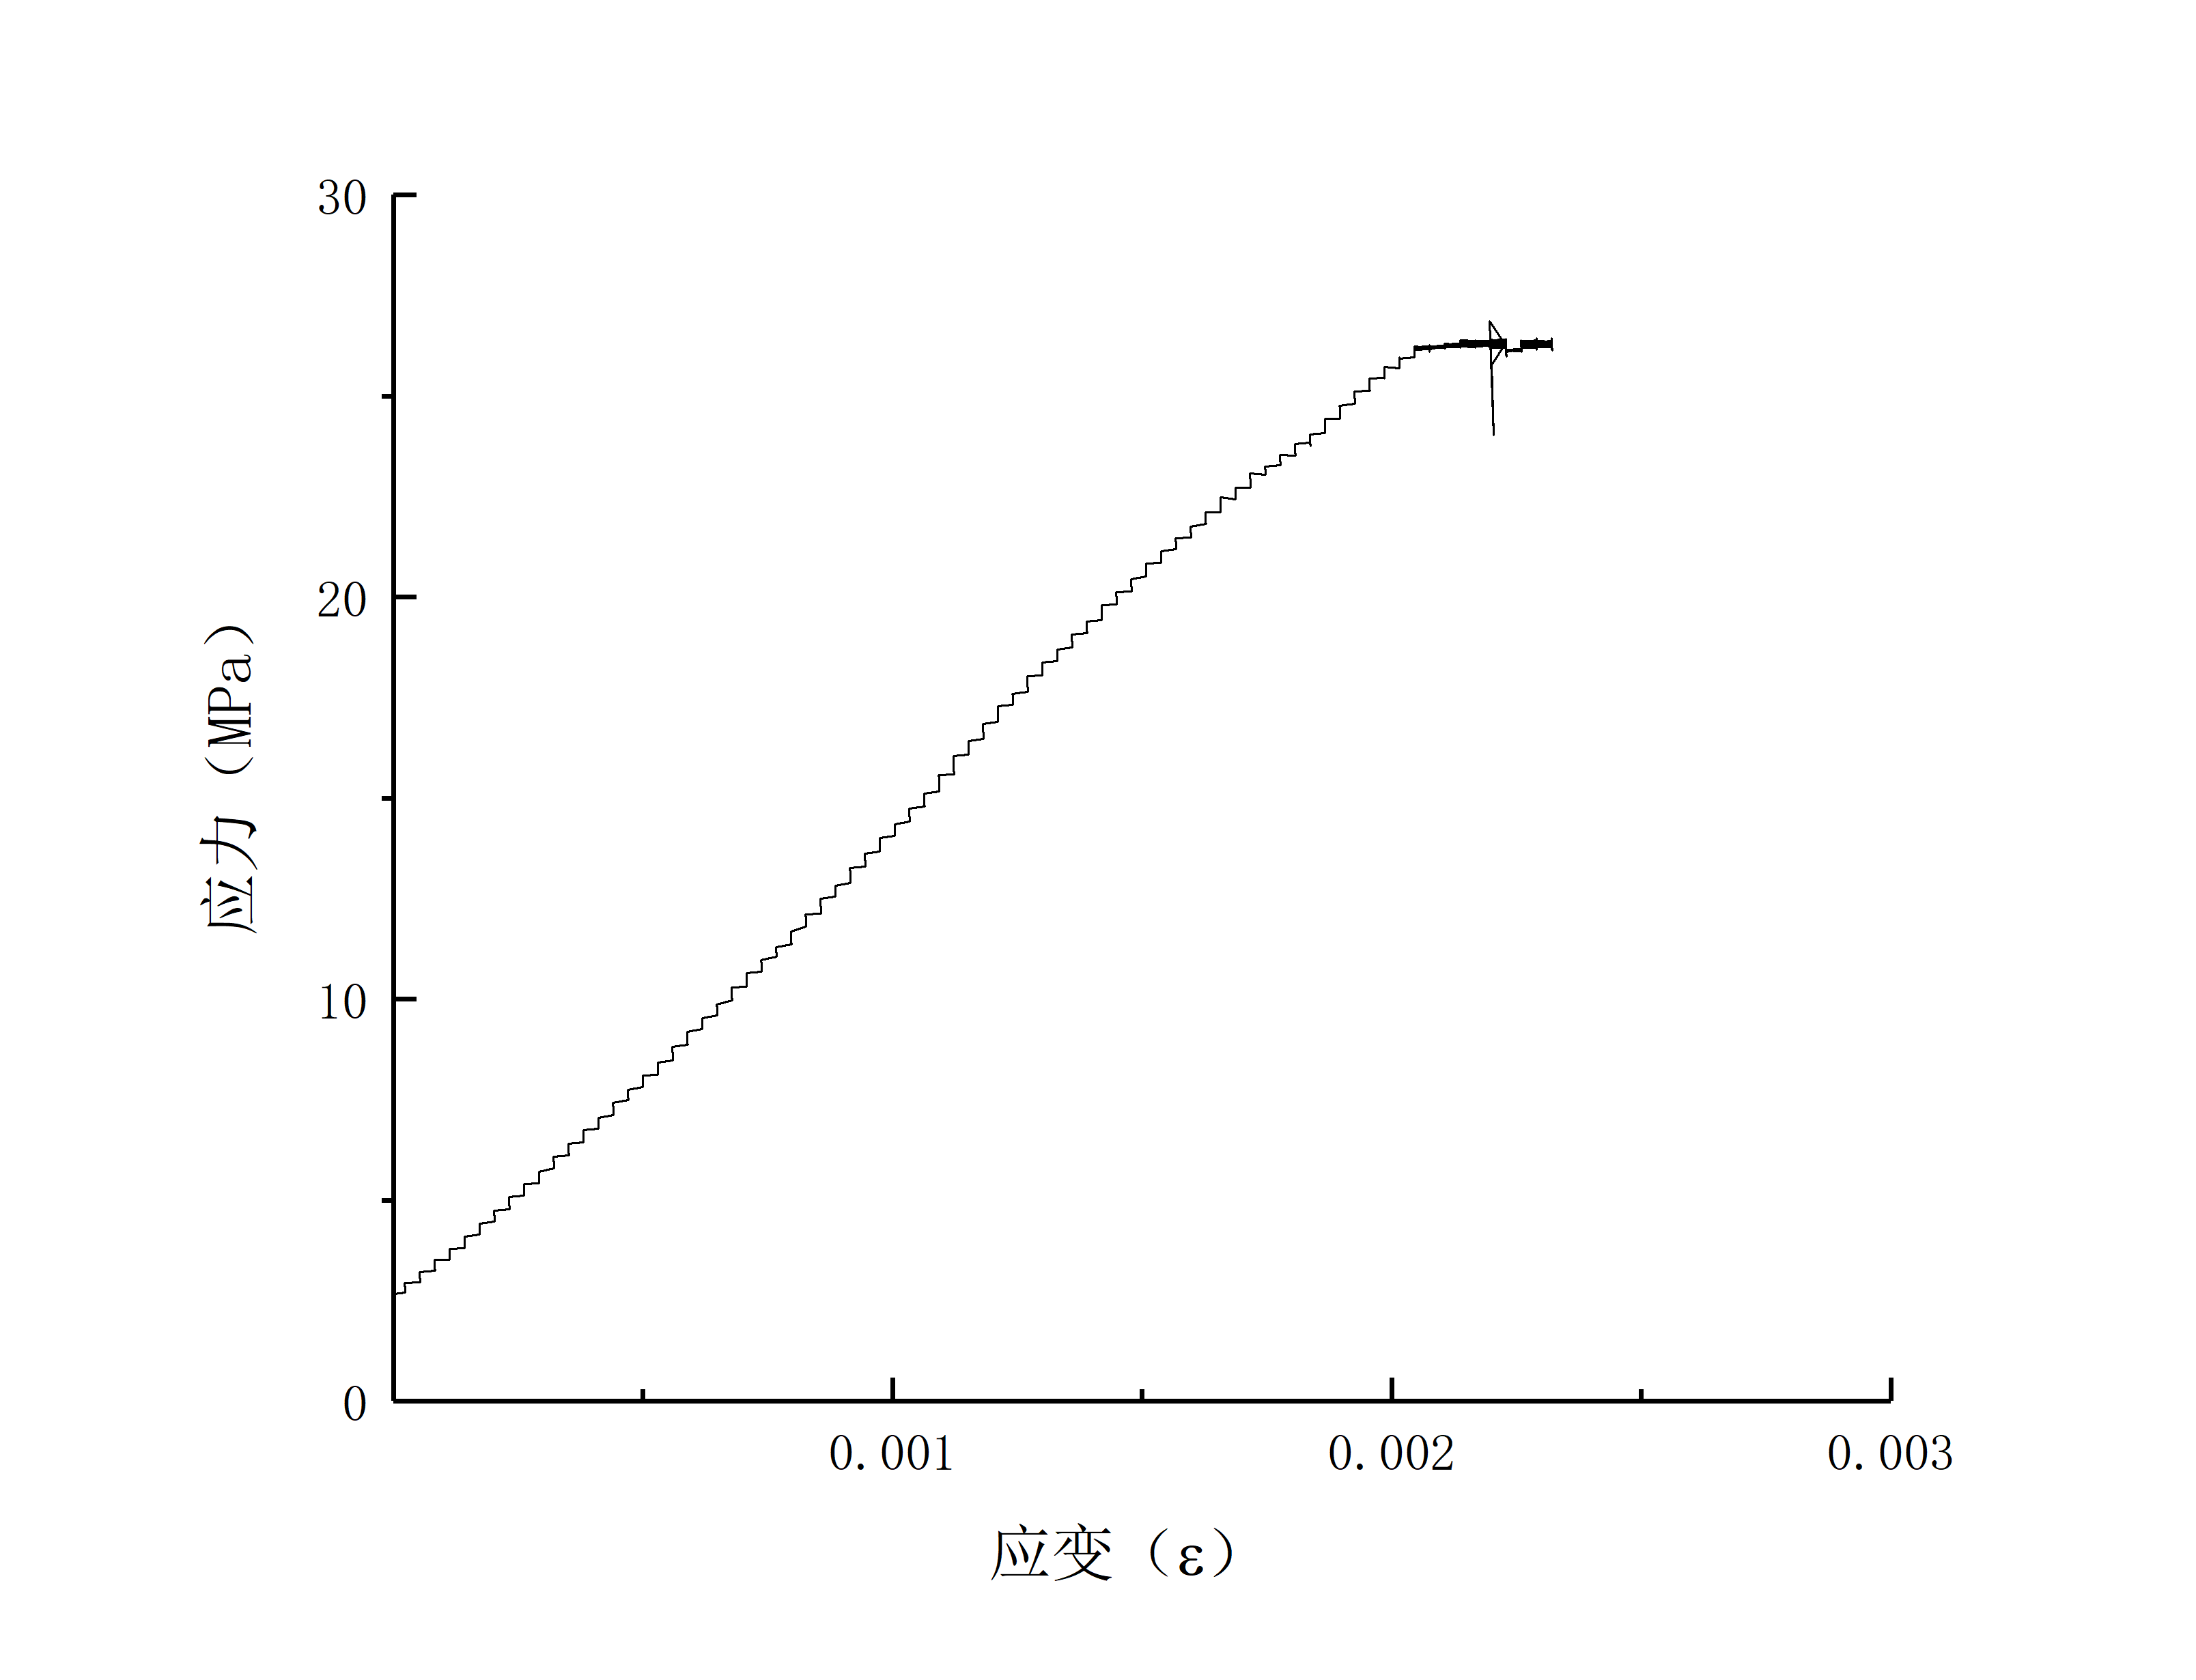
\includegraphics[width=1.1\textwidth]{img/chap2/stress-strain-C01.png}
        \end{minipage}
    }
    \subfigure[C-02]
    {
        \begin{minipage}{7cm}
            \centering
            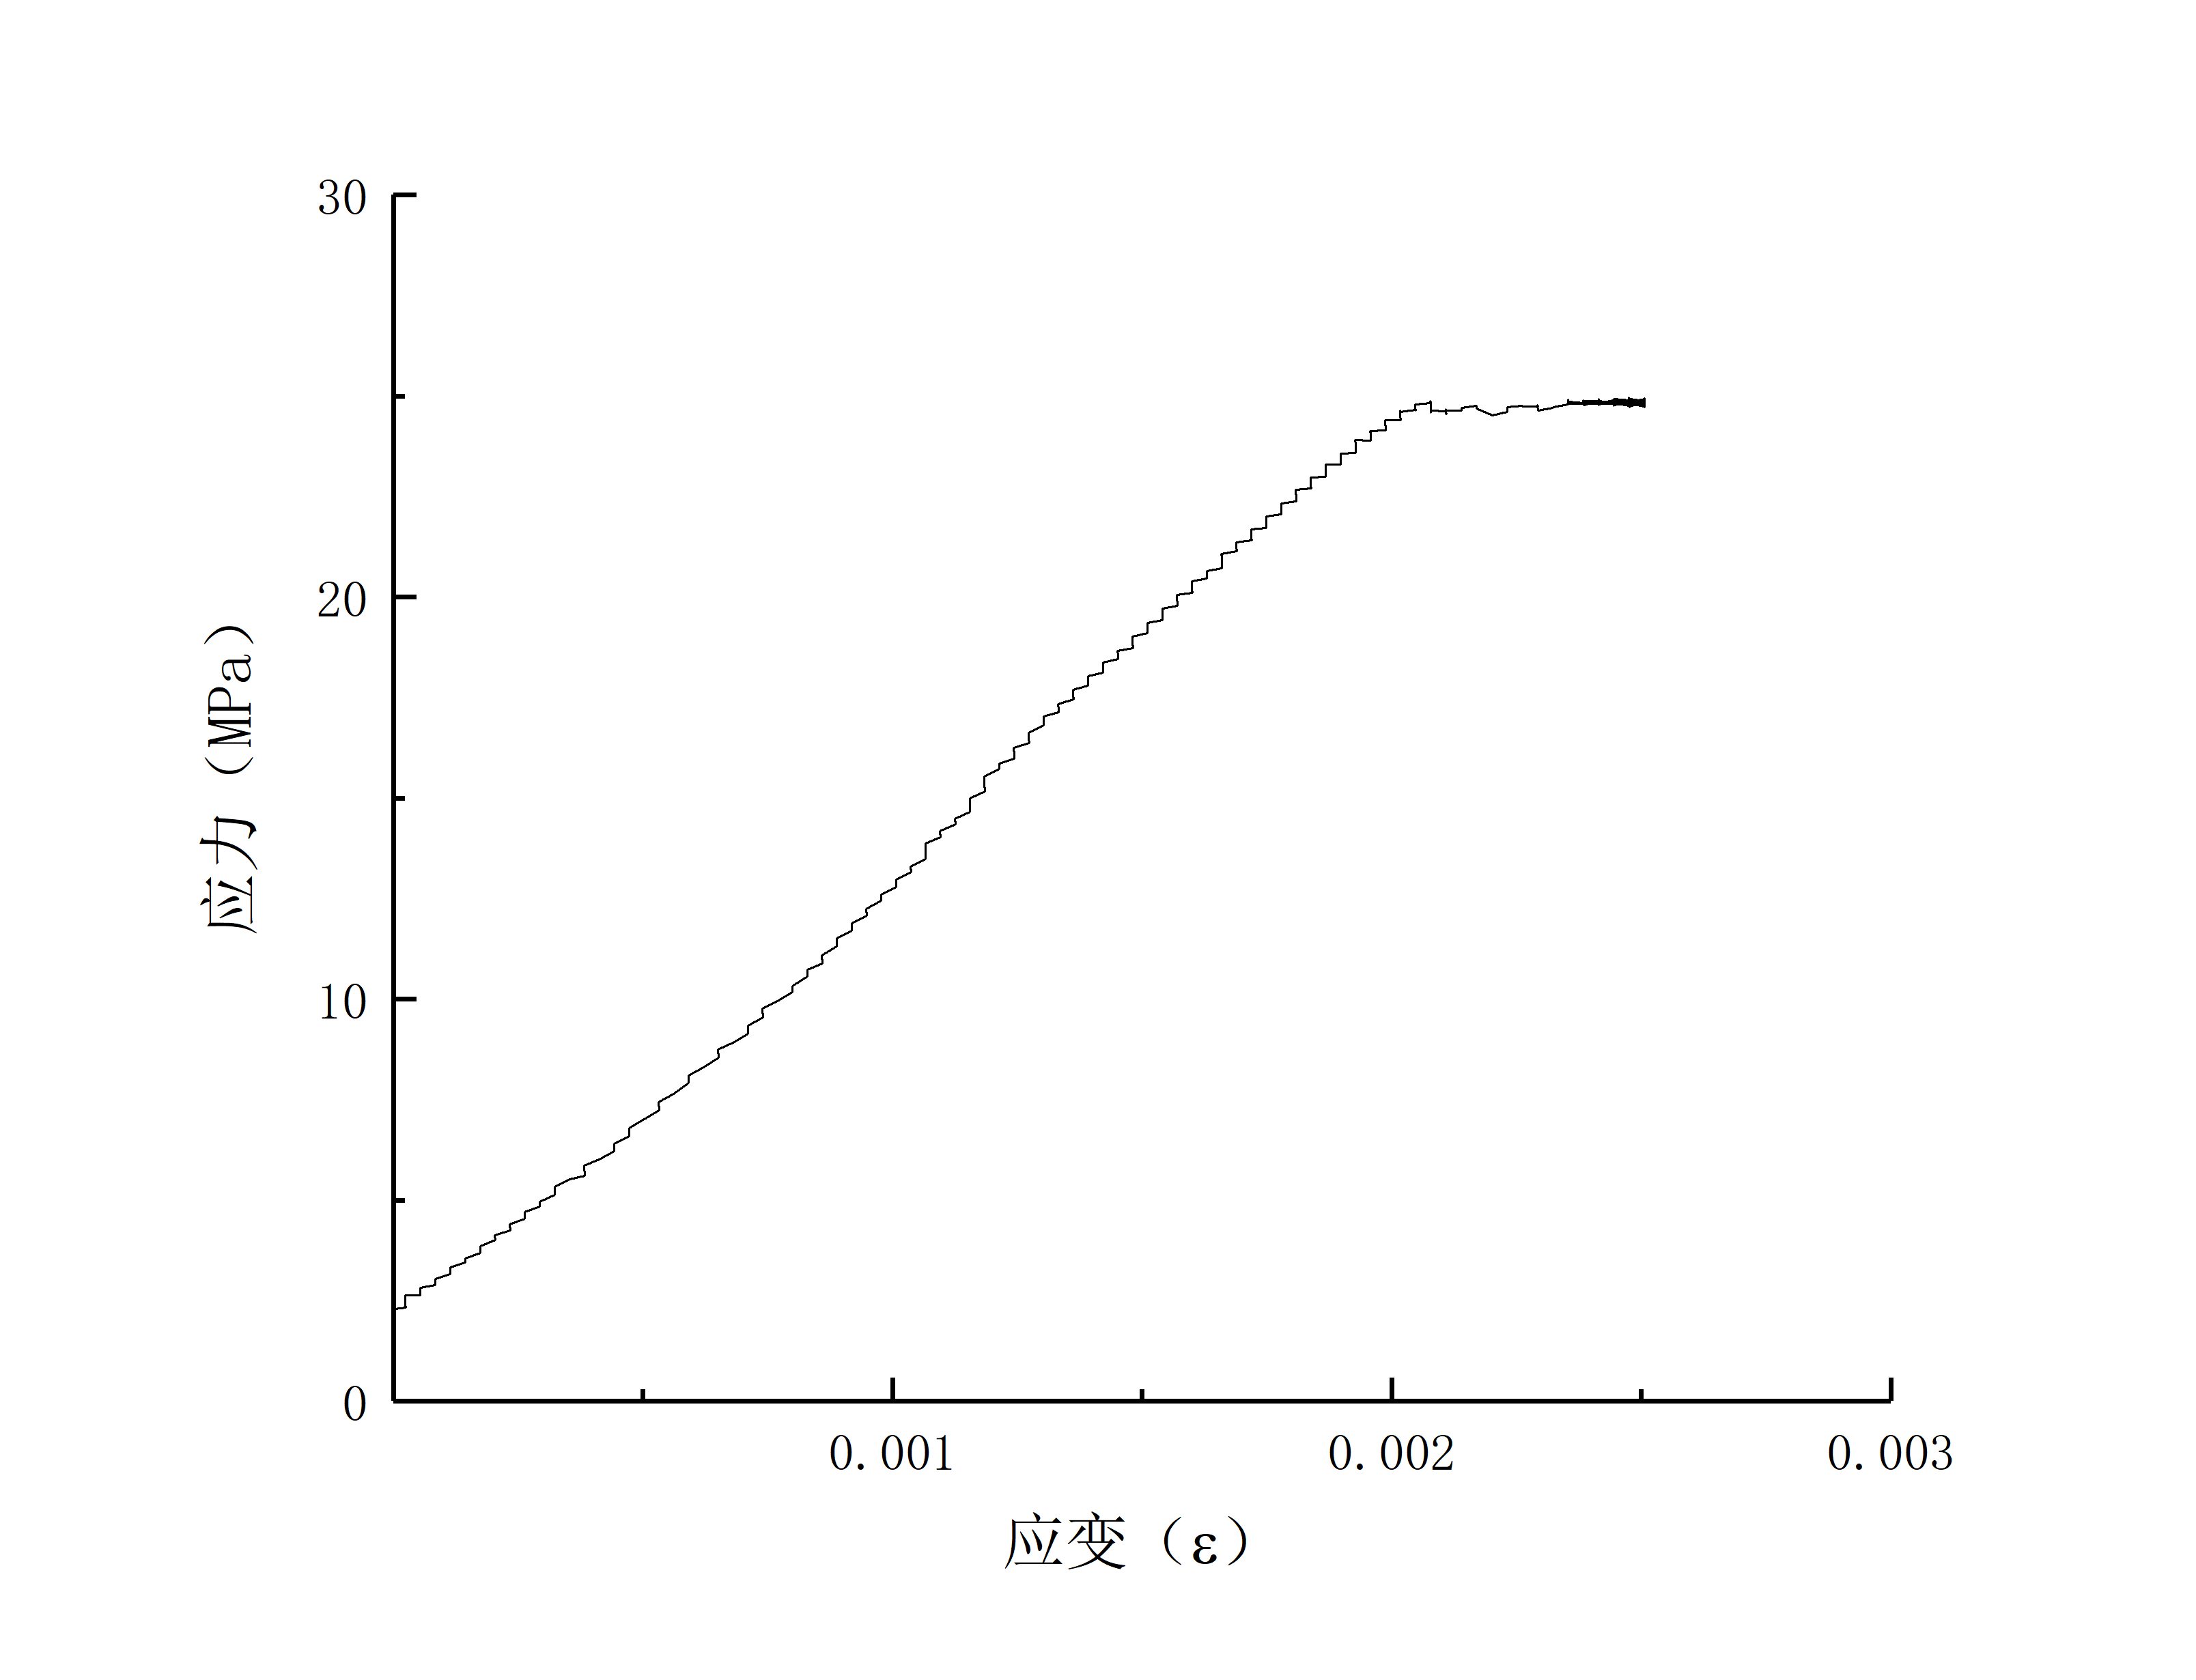
\includegraphics[width=1.1\textwidth]{img/chap2/stress-strain-C02.png}
        \end{minipage}
    }
	
    \subfigure[C-03]
    {
        \begin{minipage}{7cm}
            \centering
            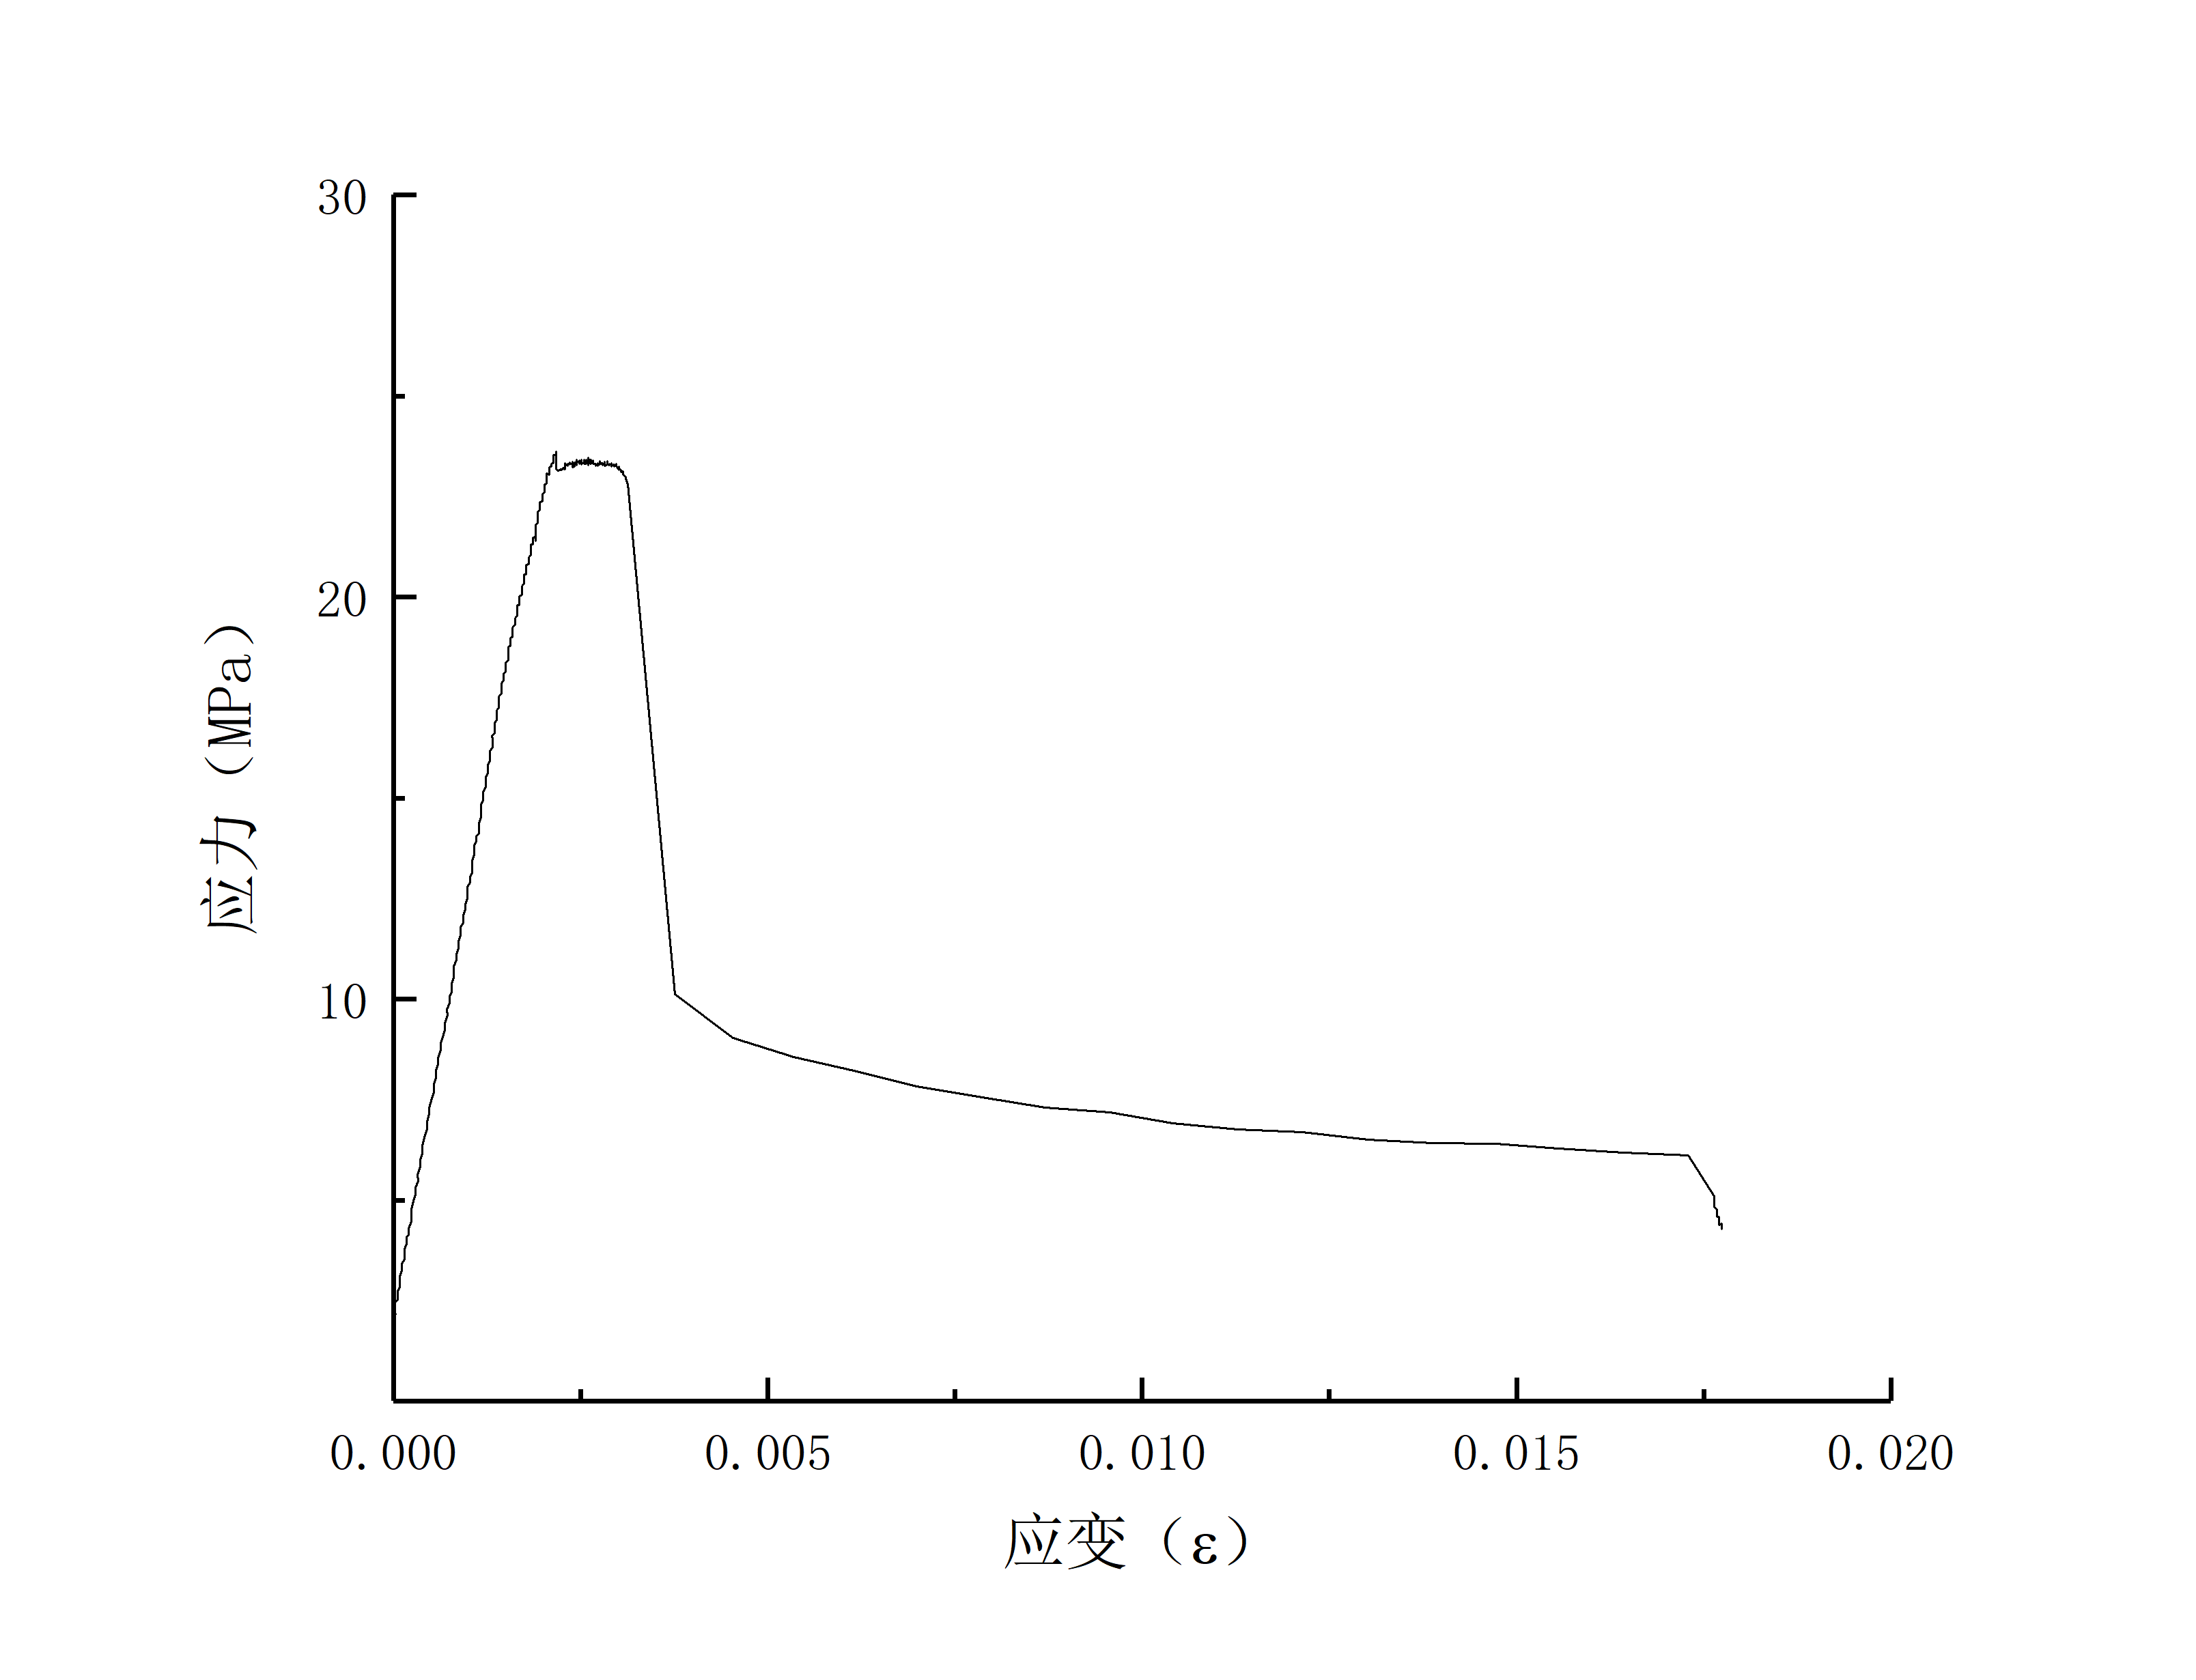
\includegraphics[width=1.1\textwidth]{img/chap2/stress-strain-C03.png}
        \end{minipage}
    }
    \subfigure[C-04]
    {
        \begin{minipage}{7cm}
            \centering
            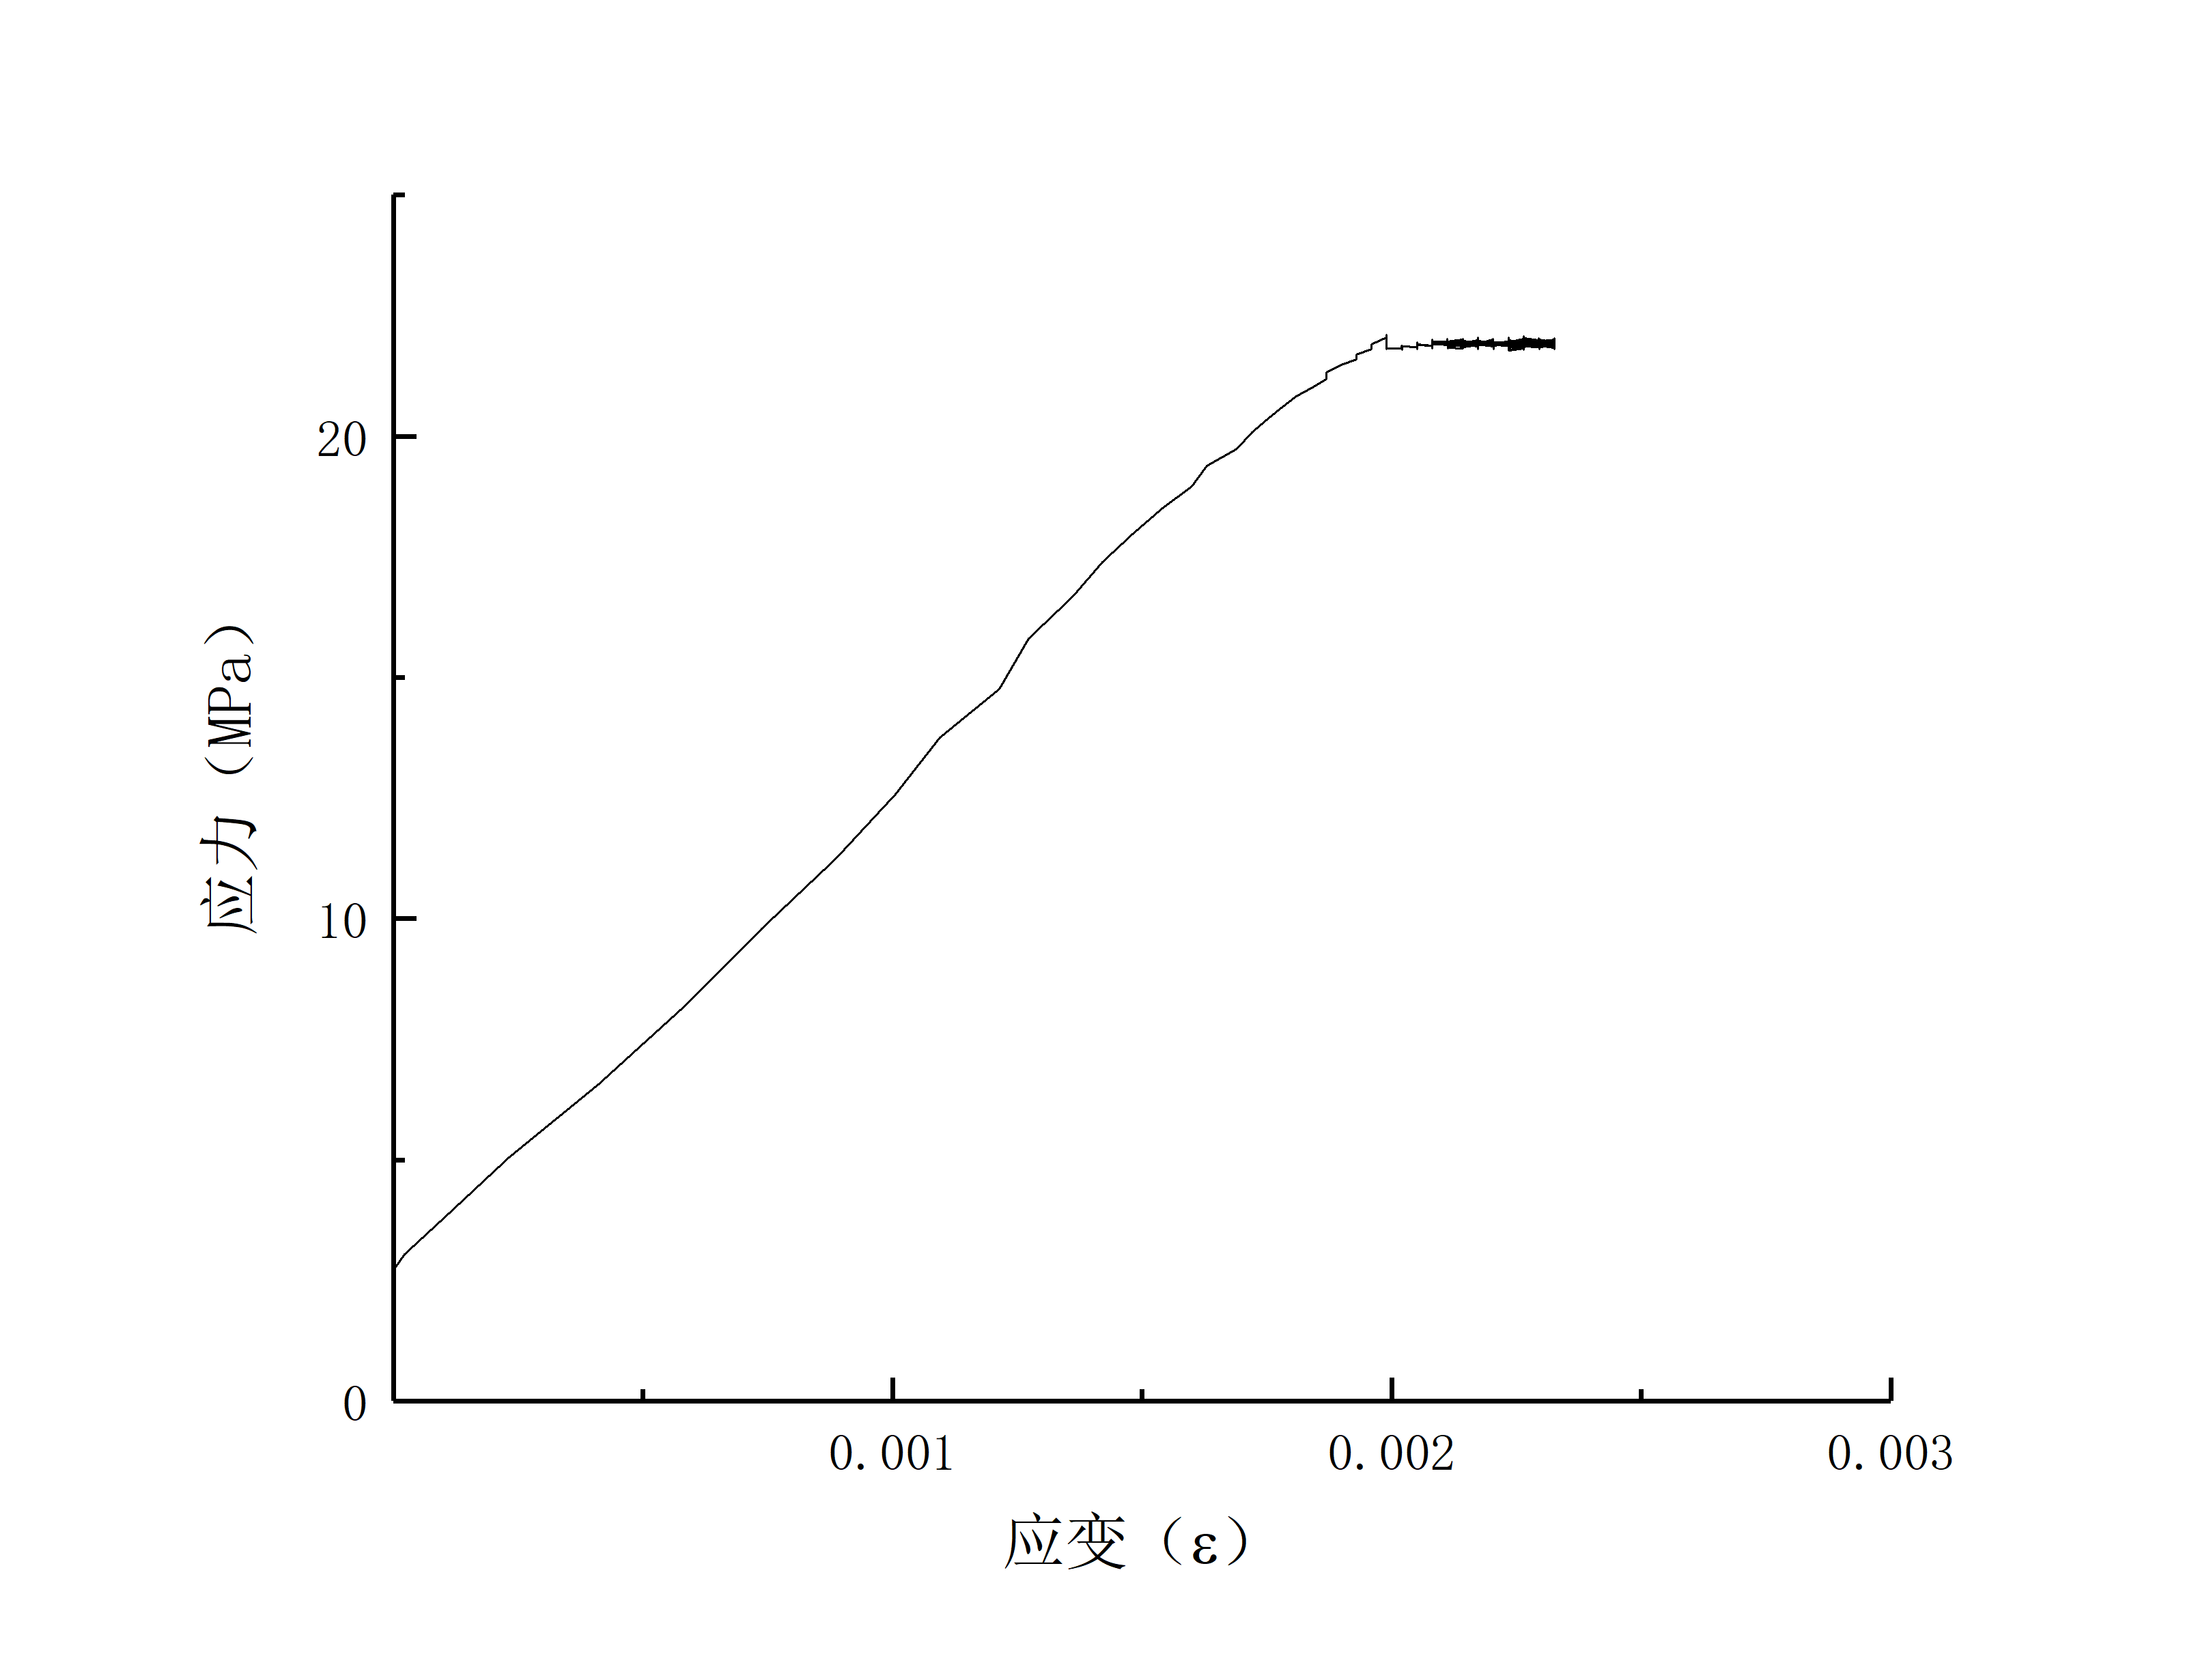
\includegraphics[width=1.1\textwidth]{img/chap2/stress-strain-C04.png}
        \end{minipage}
    }
    \centering
    \subfigure[C-05]
    {
        \begin{minipage}{7cm}
            \centering
            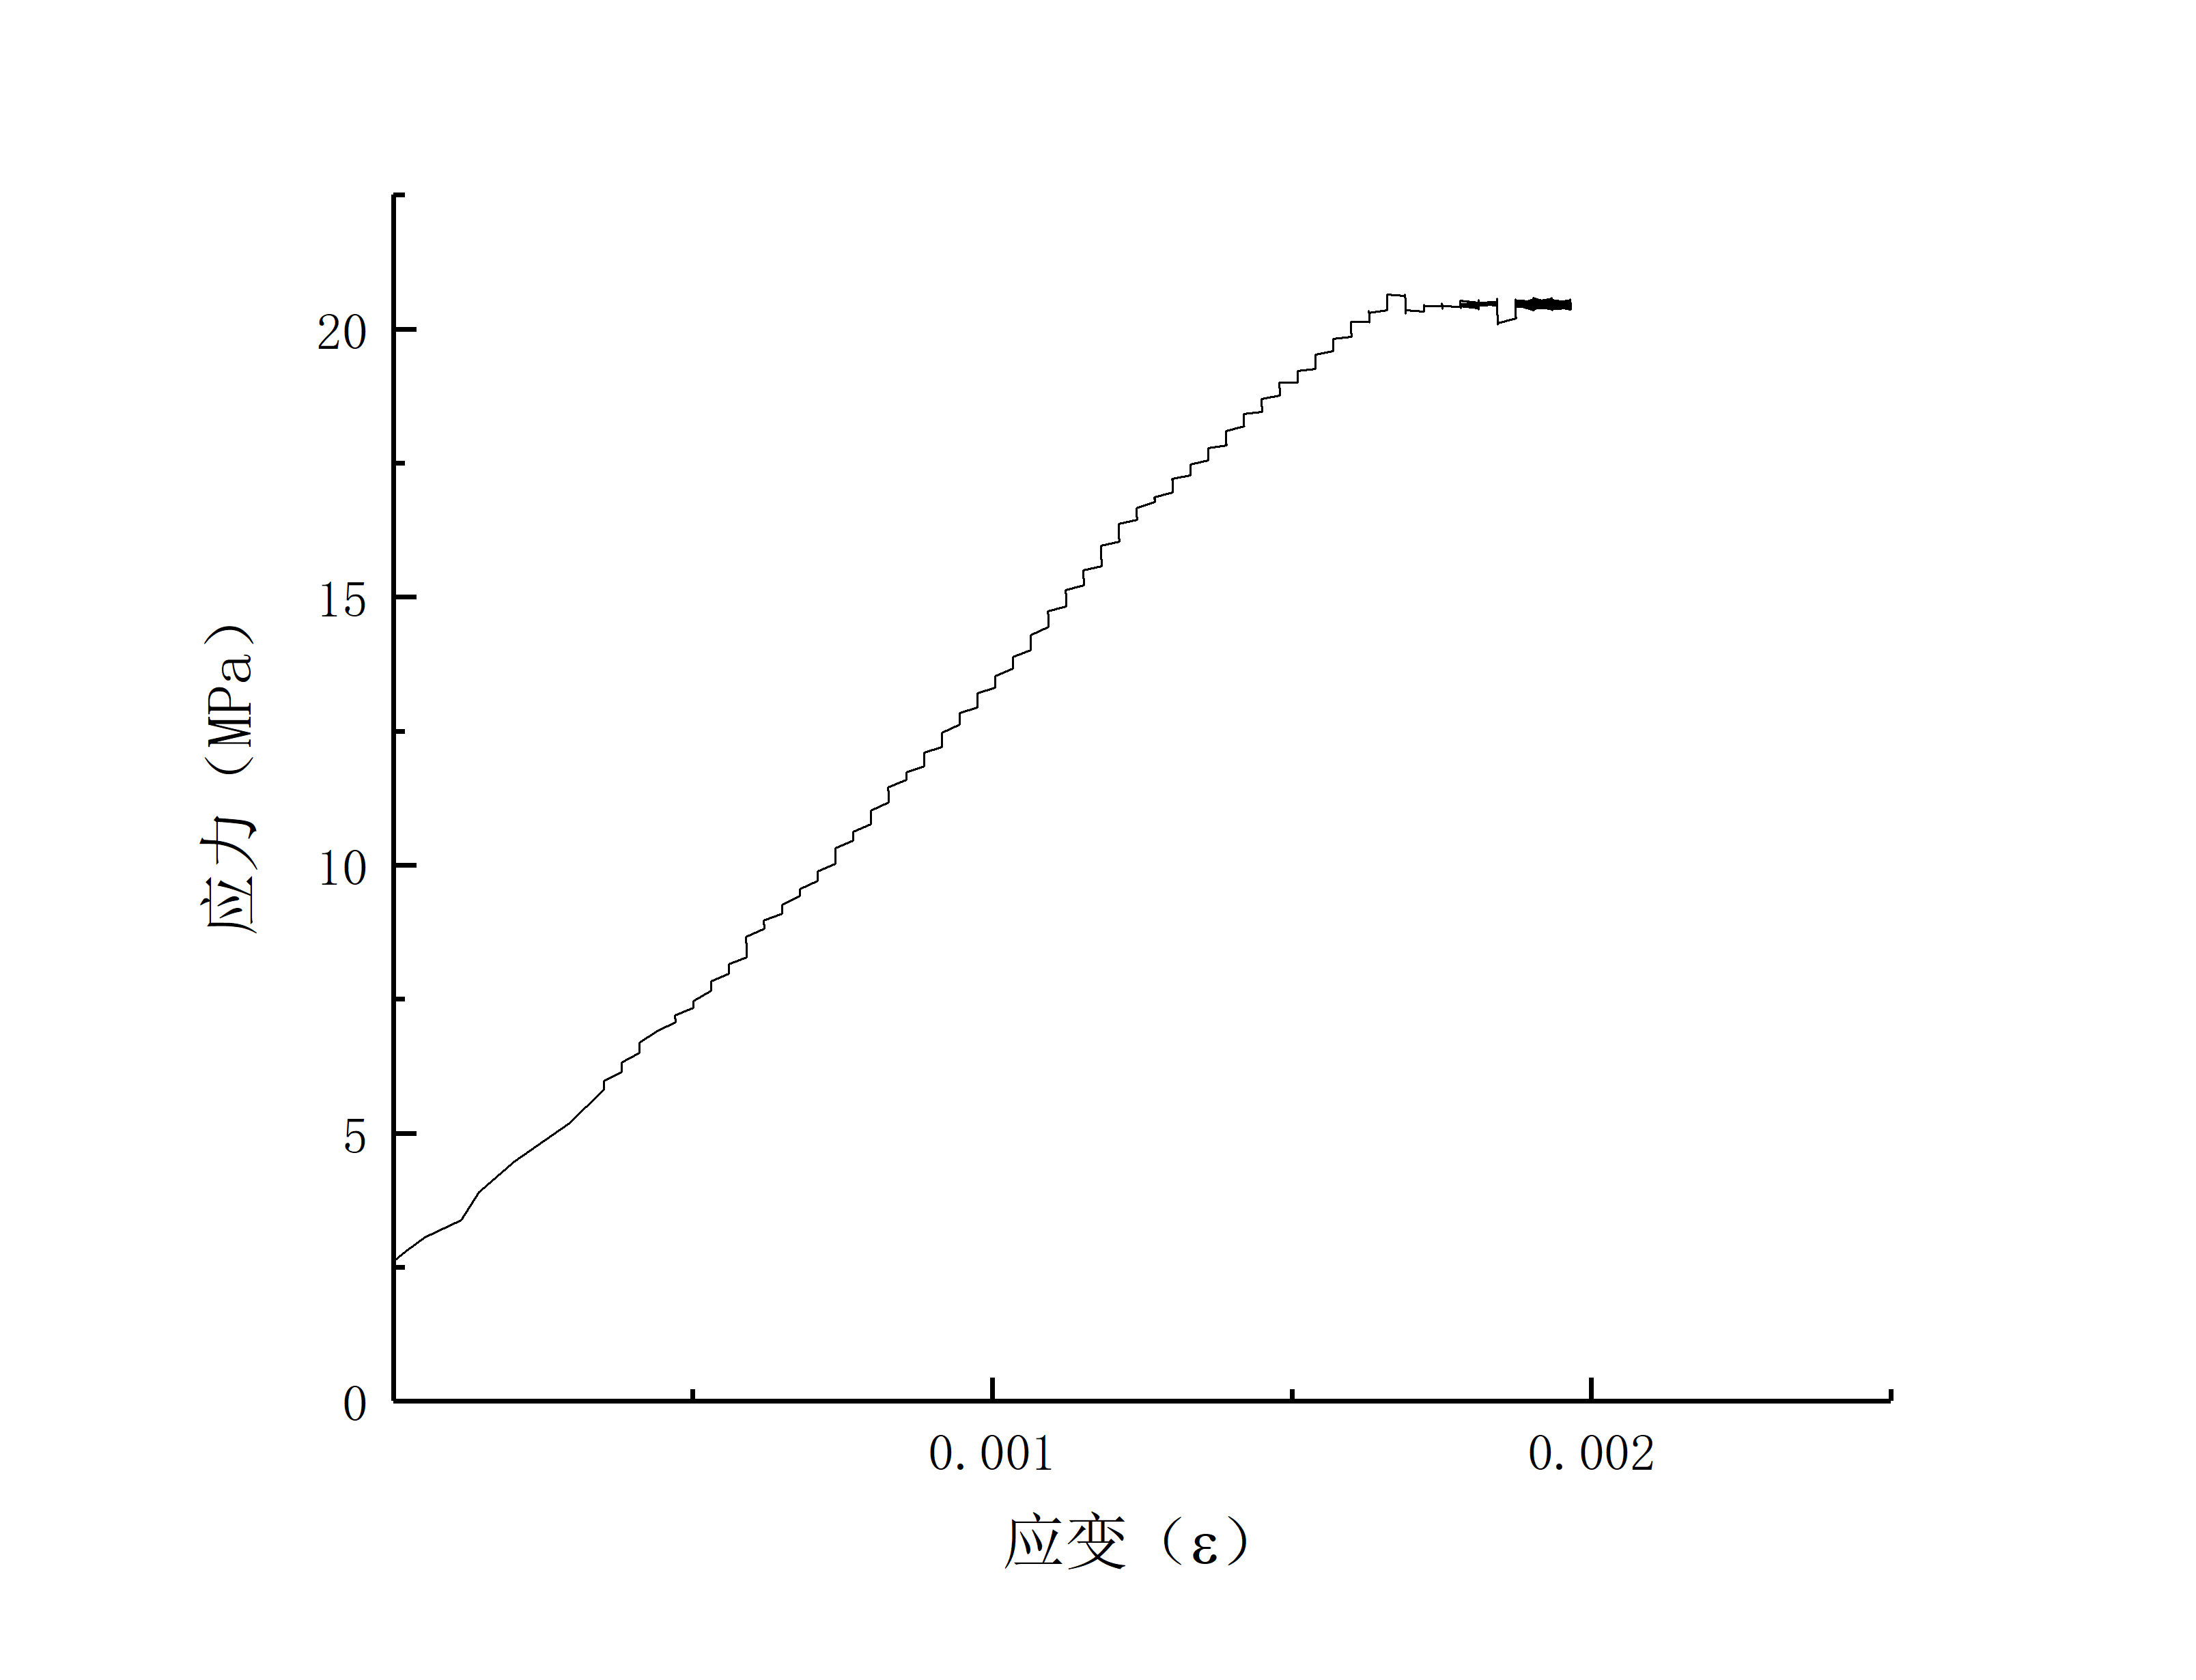
\includegraphics[width=1.1\textwidth]{img/chap2/stress-strain-C05.png}
        \end{minipage}
    }
    \centering
    \caption{单轴流变应力-应变曲线图}
    \label{fig:2-14}
\end{figure}

\section{岩石流变破裂机制探讨}
\subsection{岩石流变破裂形式}

泥岩单轴流变试验中五组试样的流变破坏形态如图\ref{fig:2-6}所示,试样在流变作用下裂纹得到充分扩展,基本表现为斜拉裂缝,局部表现为剪切破坏。而随着加载应力的增大,相应的试样上出现的裂缝也越多,说明荷载越大,流变破坏越明显。在五组试样中仅有C-03试样发生了破坏,其余四组试样仅出现了裂缝,并未完全破坏。
\begin{figure}[ht!]
    \centering
    \subfigure[C-01]
    {
        \begin{minipage}{6cm}
            \centering
            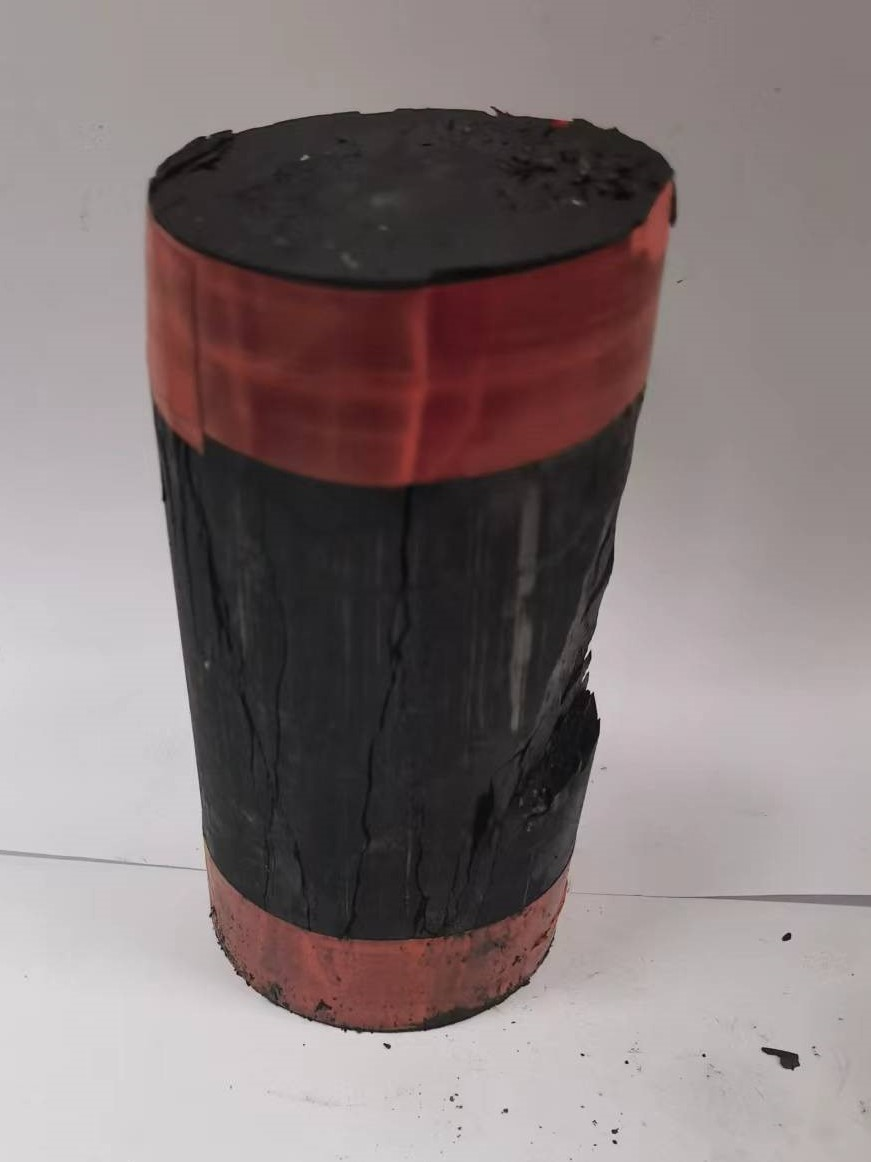
\includegraphics[width=0.9\textwidth]{img/chap2/C-1.jpg}
        \end{minipage}
    }
    \subfigure[C-02]
    {
        \begin{minipage}{6cm}
            \centering
            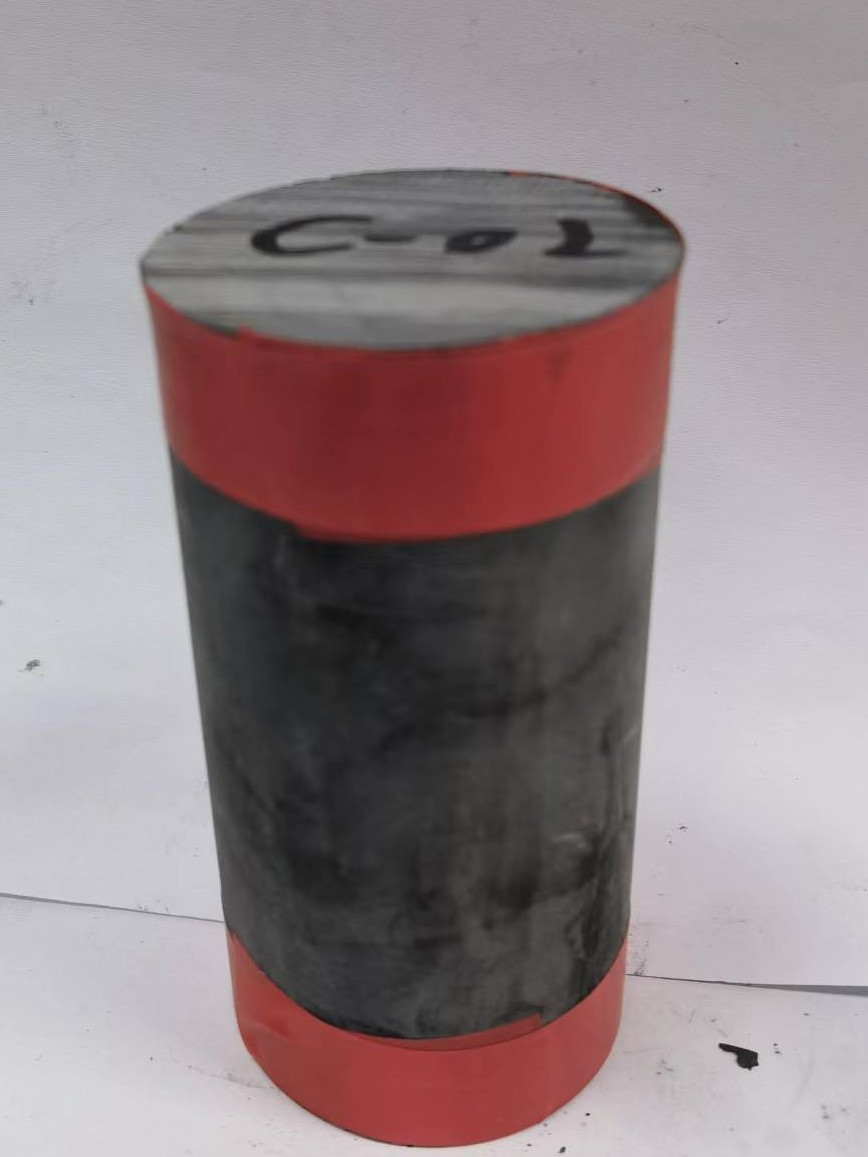
\includegraphics[width=0.9\textwidth]{img/chap2/C-2.jpg}
        \end{minipage}
    }
	
    \subfigure[C-03]
    {
        \begin{minipage}{6cm}
            \centering
            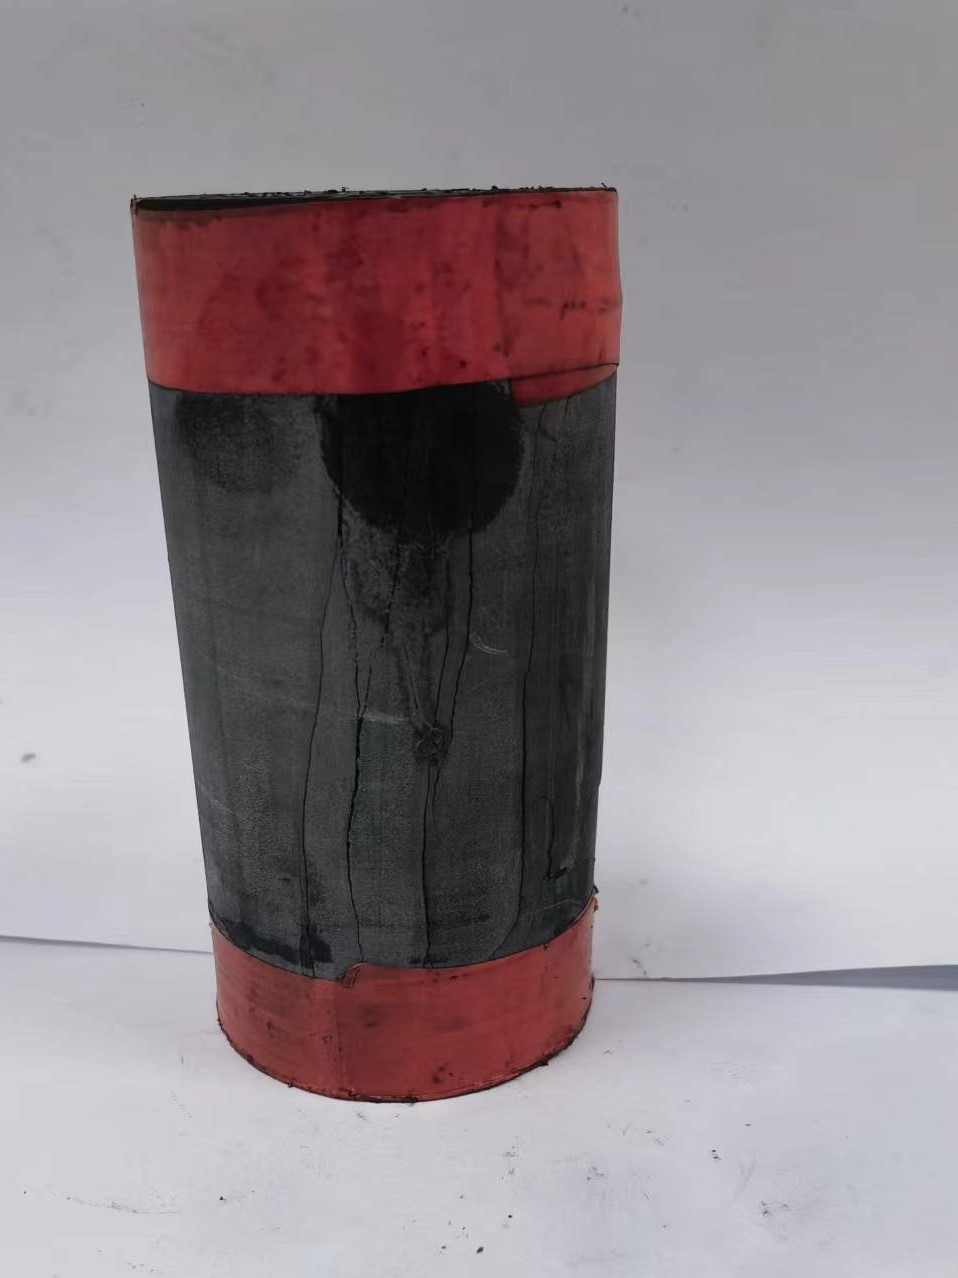
\includegraphics[width=0.9\textwidth]{img/chap2/C-3.jpg}
        \end{minipage}
    }
    \subfigure[C-04]
    {
        \begin{minipage}{6cm}
            \centering
            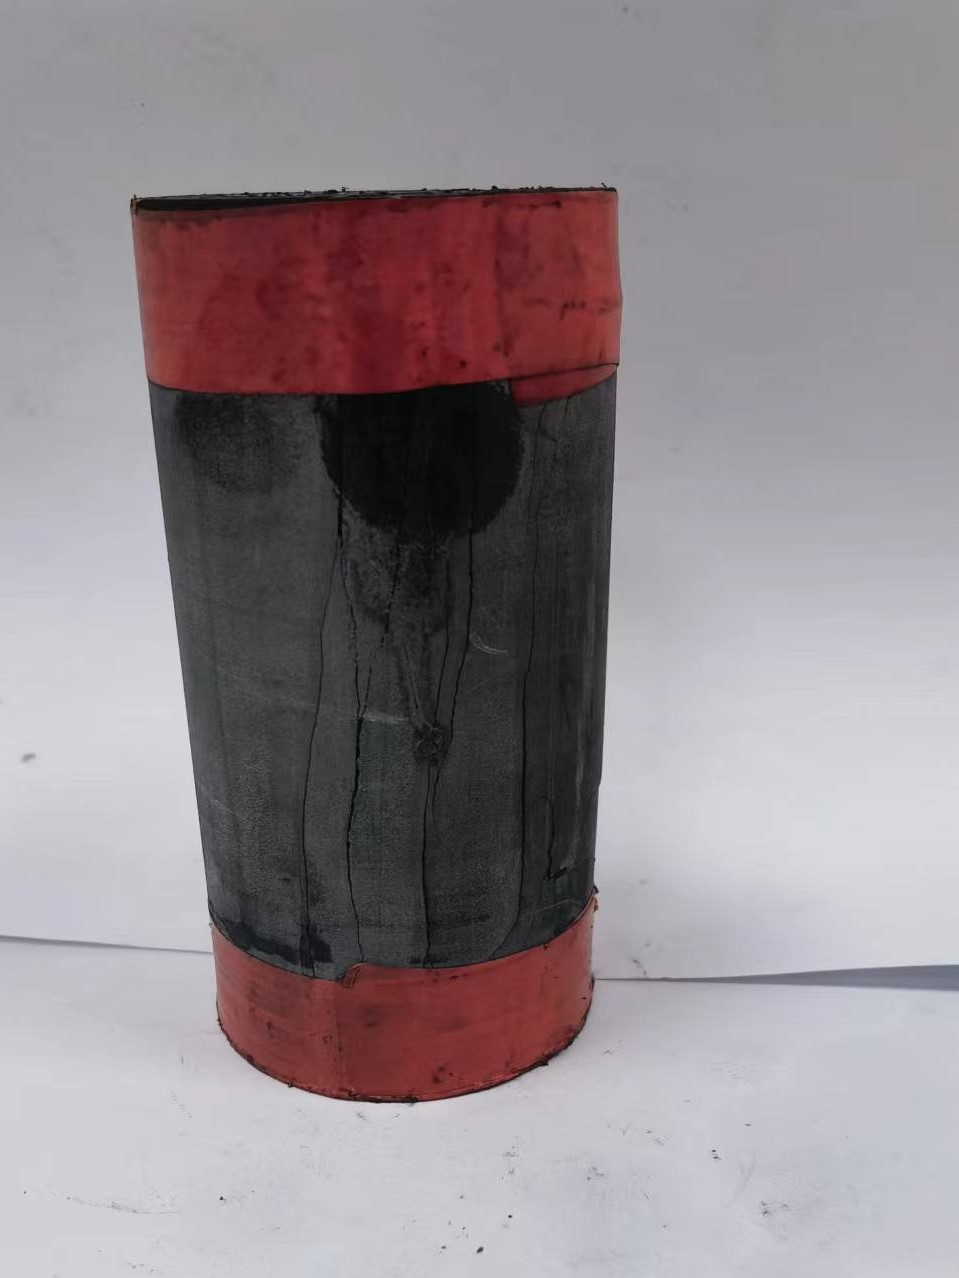
\includegraphics[width=0.9\textwidth]{img/chap2/C-4.jpg}
        \end{minipage}
    }
    \centering
    \subfigure[C-05]
    {
        \begin{minipage}{6cm}
            \centering
            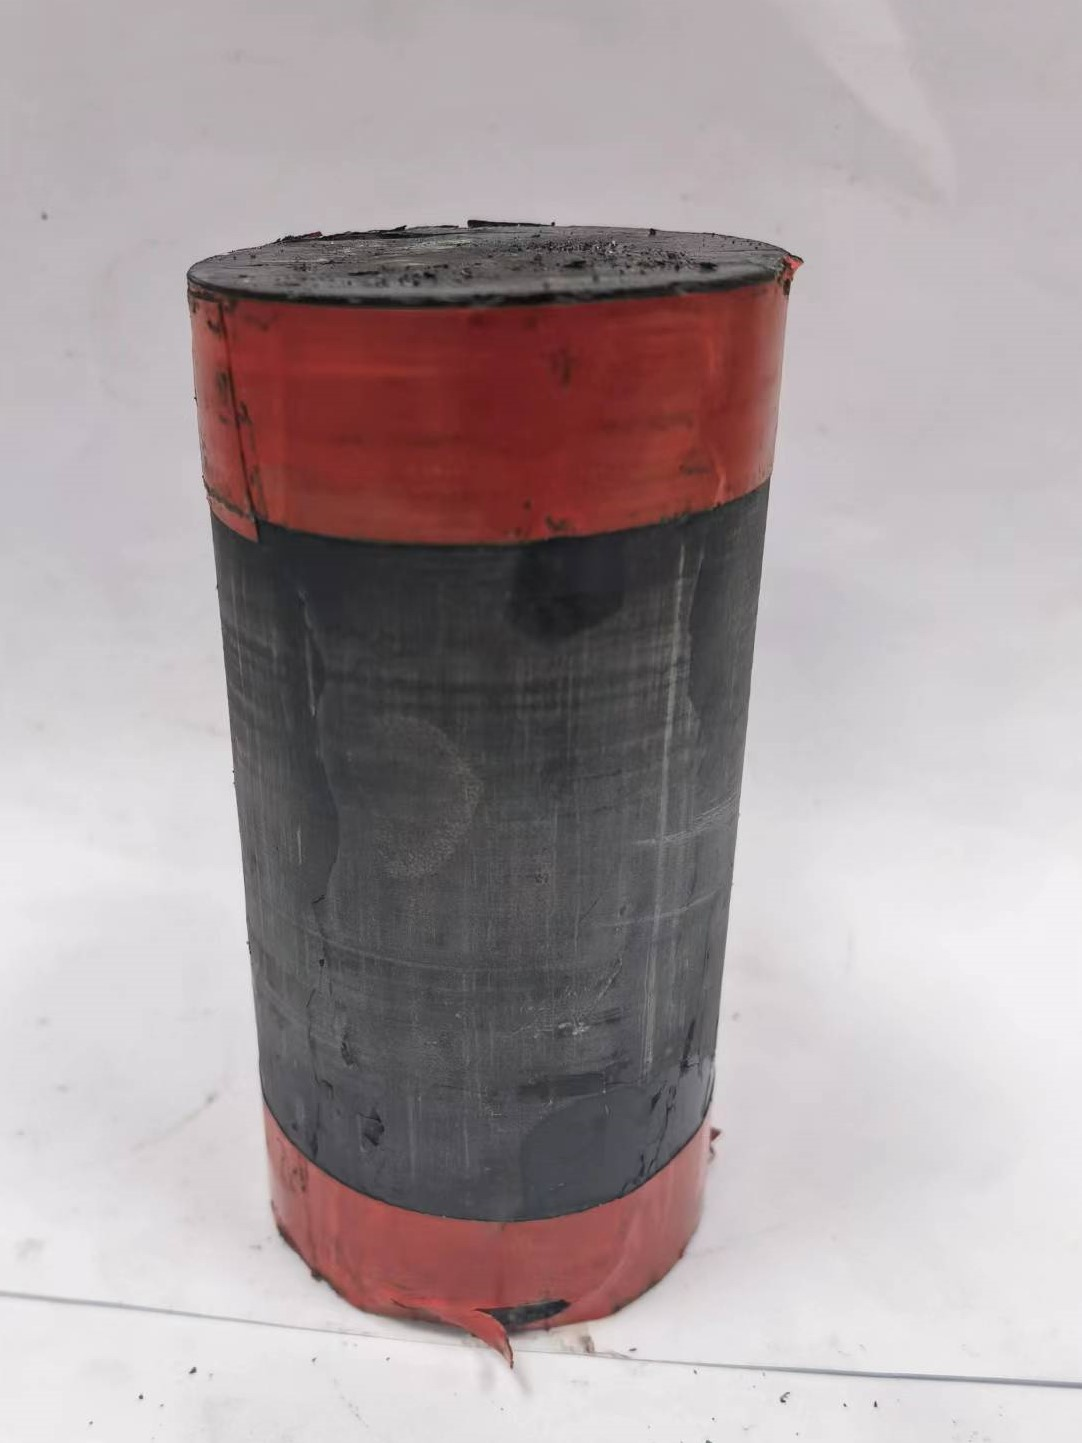
\includegraphics[width=0.9\textwidth]{img/chap2/C-5.jpg}
        \end{minipage}
    }
    \centering
    \caption{泥岩试样单轴流变破裂形式}
    \label{fig:2-6}
\end{figure}

而如图\ref{fig:2-7},在三轴流变试验中,三组试样在分级加载下均发生了结构破坏,从破坏后的试样可以看出,试验过程中均发生了剪切破坏,并伴随有部分次生剪切裂纹。在稳定蠕变阶段,裂纹以极其微弱的速度增长,主裂纹宽度有所增加,同时在试样主裂纹附近产生新的细小裂纹。在加速蠕变阶段,试样表面宏观裂纹开始互相贯通,膨胀扩容现象明显,由裂纹交织形成的细小碎片从母岩脱落。当主裂纹完全贯通,试样破坏,由动能释放产生的声响较大。

在流变试验中,裂纹的开裂扩展实质是能量耗散的过程。对岩石所做的功除累积于岩石内部的势能外,一部分在开裂过程在以粘性效应和摩擦热消耗掉,一部分以动能的形式由位错和裂纹扩展释放,常常以声发射或蠕变曲线的不规则跳动表现出来。

\begin{figure}[ht!]
    \centering
    \subfigure[D-01]
    {
        \begin{minipage}{6cm}
            \centering
            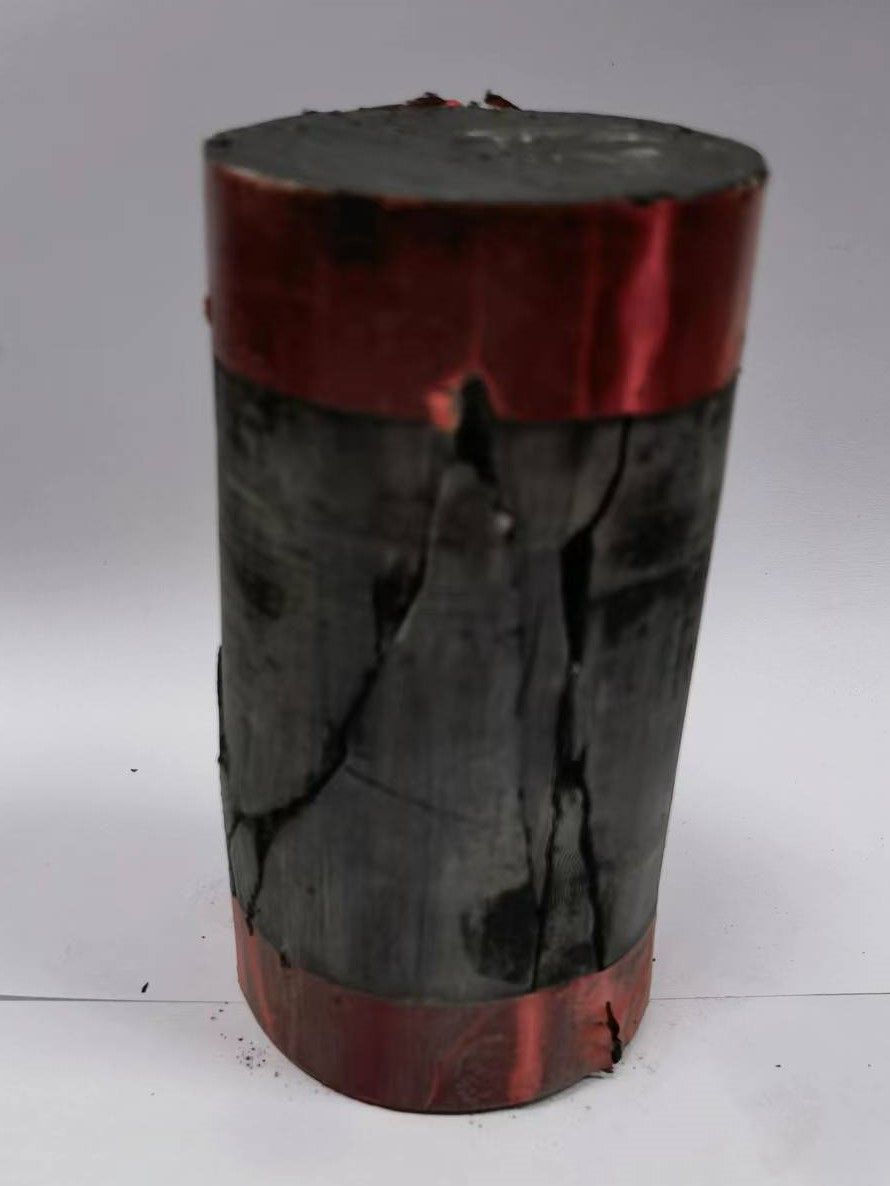
\includegraphics[width=1\textwidth]{img/chap2/D-1.jpg}
        \end{minipage}
    }
    \subfigure[D-02]
    {
        \begin{minipage}{6cm}
            \centering
            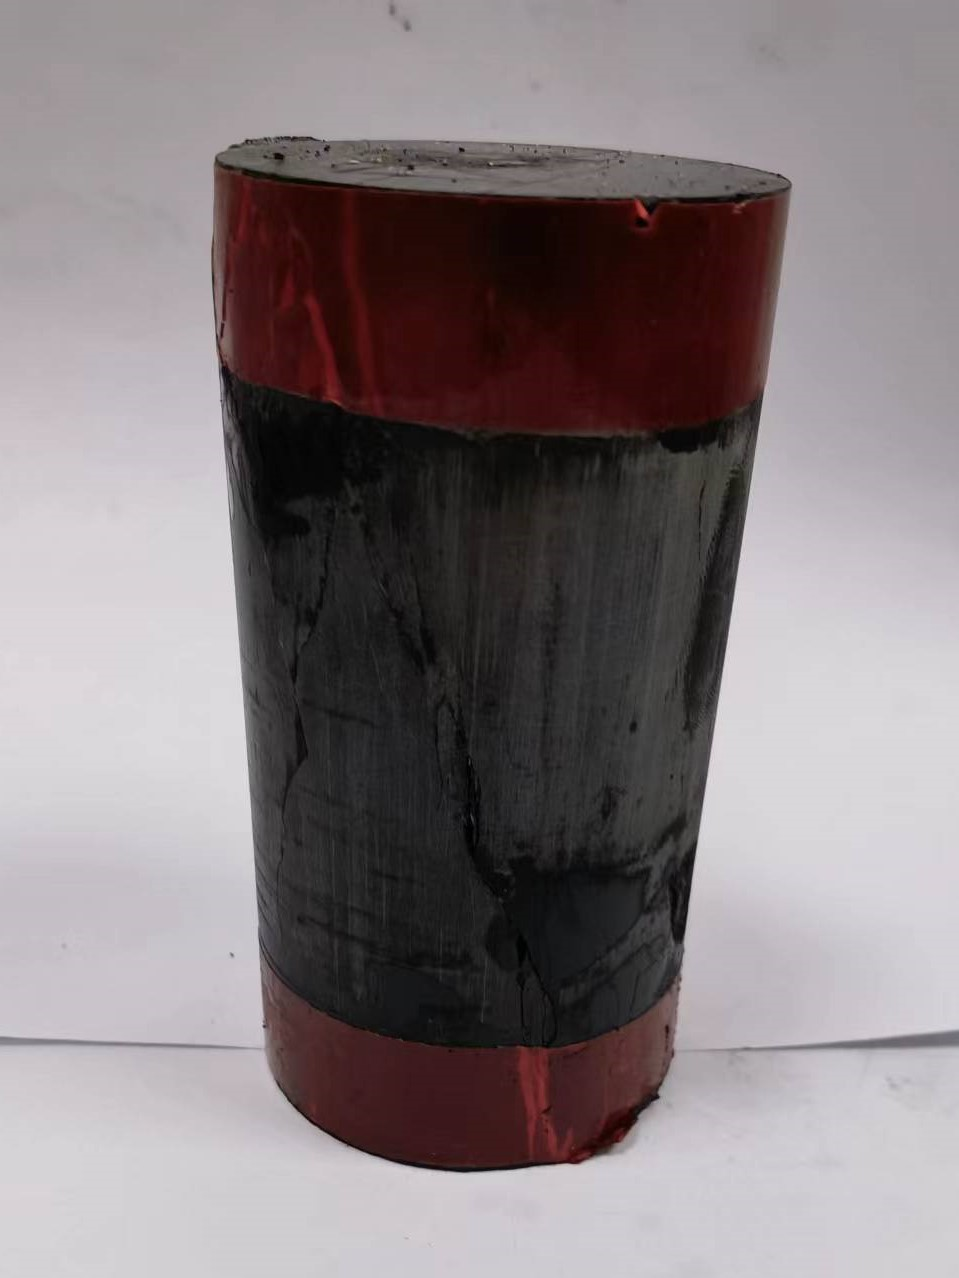
\includegraphics[width=1\textwidth]{img/chap2/D-2.jpg}
        \end{minipage}
    }
	
    \subfigure[D-03]
    {
        \begin{minipage}{6cm}
            \centering
            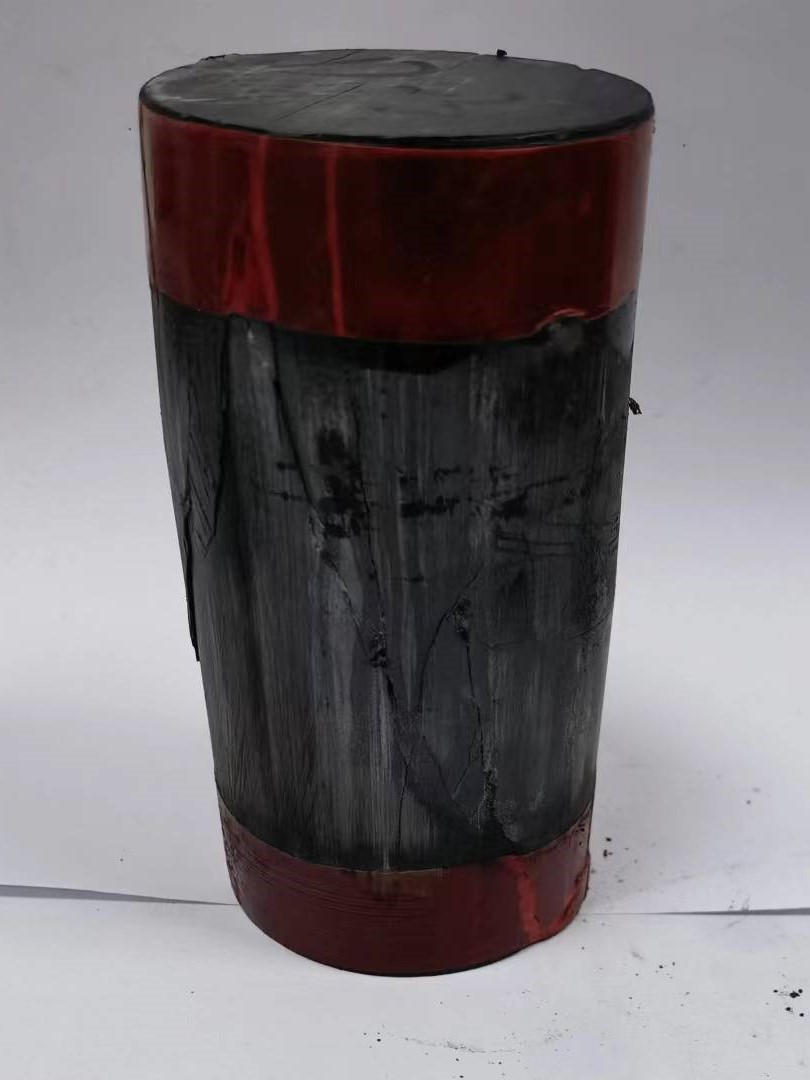
\includegraphics[width=1\textwidth]{img/chap2/D-3.jpg}
        \end{minipage}
    }
    \centering
    \caption{泥岩三轴流变破坏形式}
    \label{fig:2-7}
\end{figure}

\subsection{泥岩微观流变破裂机制探讨}

上一节阐述了试样宏观上的破坏形式,然而该过程只占整个流变全过程很短的时间,大部分时间均为岩石内部微裂纹、微结构变化发展的过程,这也是形成宏观裂纹的前提,要深入分析岩石流变破坏就必须对微裂纹、微结构的演化机理分析研究。

对于流变损伤断裂的研究多见于金属等晶体的变形过程。晶体在位错滑移过程中遇到障碍物塞积,产生硬化,同时在位错塞积群附近发生应力集中,产生张性裂纹。外力的驱动也可能使晶粒内发生空位扩散,空位绕晶粒边界扩散或穿晶扩散。岩石作为一种多晶复合介质,与金属的流变损伤机制有所不同,可将其内部划分为三种类型:晶粒内部、晶粒界面、晶粒间隙。晶粒由于扩散蠕变而变形并沿粘性晶界互相滑动,晶界处微孔由于空位扩散而成核,并汇集成断裂轨迹。微孔成核过程中一些物质扩散并淤积于晶粒边界,削弱晶粒间的联结,形成“蚀变带”。晶界上微孔成核的过程即为材料流变损伤的过程。

不同种类的岩石,由于组成结构不同,其微细观流变破裂机制有所差别。泥岩中黏土颗粒含量较高,这些细小的黏土颗粒构成了较大的集粒,相互交织定向排列,呈絮凝状结构,单元体以细小颗粒构成了较大的集粒,
它们相互交织呈定向排列,这种结构反映了泥岩主要由黏土矿物组成的特性,其孔隙存在于絮凝状结构之间,分布较为均匀。

在初始蠕变阶段,泥岩中的粗粒晶体几乎不产生变形及位错滑移,主要为初始微孔、微裂纹的闭合,黏土类胶结物被压缩咬合,泥岩得到硬化,结构强度提高。在第二蠕变阶段,黏土类胶结物出现弱化,微孔、微裂纹开始等速扩展,结构破坏逐渐增多,应力不断调整。在此阶段虽然损伤不断发展,但是结构硬化和损伤始终保持动态平衡。在加速蠕变阶段,黏土类胶结物被破坏,黏土物质与粗粒晶体分离并形成空洞,晶体颗粒互相错动,结构大量破坏。此时损伤积累完成并呈现加速发展,当由微缺陷组成的裂隙贯通时,岩样发生破坏。

岩石的蠕变破坏过程就是岩石内部应力不断调整的过程,也是硬化与软化相互作用的过程。在蠕变初始阶段,微孔隙闭合、软弱相的压缩及颗粒协调变形使岩石强度提高,硬化占据主要地位。在第二蠕变阶段,随着微裂隙的扩展损伤逐步积累,软弱相破坏退出工作,应力不断调整,蠕变规律随损伤速率等速变化。在第三蠕变阶段,微裂隙累积形成宏观细裂纹并贯通形成主裂面,损伤呈非线性加速发展,岩石蠕变破坏。


\section{小结}
本试验以泥岩为研究对象,通过开展常规单轴、三轴压缩试验获得泥岩的基本物理参数,再通过室内单、三轴流变试验研究泥岩的流变特性,得出的主要结论如下:

(1)通过开展常规单、三轴压缩试验,发现泥岩应力—应变曲线三个主要阶段——弹性变形阶段、微裂隙发展阶段、破坏阶段的变形特征,得到了泥岩的弹性模量、泊松比等基本物理参数。泥岩试样在常规压缩试验下的破化特征主要呈现出纵向的劈裂、张拉破坏以及局部的剪切破坏,而泥岩在流变试验下呈现出的主要为剪切破坏形态。

(2)通过对Boltzmann叠加原理对三轴流变试验的阶梯型流变曲线进行处理。

(3)通过处理完成的单、三轴流变试验的时间-应变曲线,我们可以发现流变变形量随应力等级的提高而增加,随着应力等级的提高,泥岩的流变变形量以及残余应变值也在逐渐增加。在本次试验中,岩泥在加载瞬间产生的瞬时变形,随后进入衰减和稳定蠕变的阶段,稳定蠕变阶段历史最长但流变变形量小。
试验时施加的应力越大,初始流变速率及稳态流变速率也呈递增趋势,流变速率在初始蠕变阶段内不断减小,在稳定蠕变阶段达到一个保持不变的数值,在较低的应力下,稳定蠕变速率将会无限接近于0。

(4)本次实验中,在单轴流变实验中未出现加速蠕变阶段。在三组三轴流变试验中,在最后一级应力加载下均出现了加速蠕变阶段,加速蠕变阶段虽然流变历时较短,但流变变形量远大于前几级应力下的流变量。

(5)岩石试样的破裂形式主要表现为轴向张拉破坏,局部表现为剪切破坏。宏观破坏主要集中在加速蠕变阶段,裂纹互相交织形成贯通试样的破裂面,膨胀扩容变形现象明显。微观条件下,初始微缺陷产生的位错、滑移与晶体颗粒协调变形构成软化与硬化两种机制相互竞争的局面。当内部微缺陷、微裂纹由于长期损伤积累已经占据主要地位时,原有胶结结构破坏,黏聚力丧失,损伤呈非线性加速发展,微裂纹汇聚形成宏观裂纹,岩石蠕变破坏。









%
    \chapter{泥岩流变本构模型及参数拟合}

\todoiZN{这一章要重新梳理,不然查重过不了}
\label{chap:theory}
岩石流变本构模型的建立一直是岩石流变力学理论研究的重点和难点,
合适的本构模型能够较为准确地描述岩石的本质特征,并能较为准确地反映岩石的力学特性和变形机理。因为岩石材料种类繁多,所以流变规律和流变本构模型的表现形式应是多样的,要找到一种普遍适用的、能够全面反映岩石流变力学特性及变形机理的本构模型基本是不可能的。因此,针对工程的实际情况建立适用于该工程本身的本构模型具有重要的意义。目前,建立岩石流变本构模型的方法主要有经验模型、元件模型以及根据热力学内时理论、损伤断裂力学等理论建立岩石的流变本构模型。

\section{流变本构模型}

\subsection{经验模型}
岩石经验流变模型是在岩石流变试验的基础上,通过假设——实验——理论的方法来建立岩石的应力、应变和时间的函数关系模型。经验型蠕变本构模型往往采用幂函数、对数函数、指数函数、双曲线函数等数学表达式。此类模型虽然较为直观,应用方便,但其只是通过流变表观现象获得,物理意义不明确,只适合描述在特定试验条件下的流变行为。

岩石的典型蠕变曲线是通过大量的岩石单轴压缩蠕变试验,在恒定应力水平 作用下,总结出来的岩石随时间的变形规律,其蠕变方程可表示为:
\begin{equation}
     {\varepsilon}={\varepsilon}_{0}+{\varepsilon}_{1}+{\varepsilon}_{2}+{\varepsilon}_{3}
\end{equation}

式中,$\varepsilon$为总应变,$\varepsilon_0$为瞬时应变,$\varepsilon_1$、$\varepsilon_2$、$\varepsilon_3$分别为衰减蠕变阶段、等速蠕变阶段和加速蠕变阶段的应变。

\begin{figure}[ht!]
    \centering
            \centering
            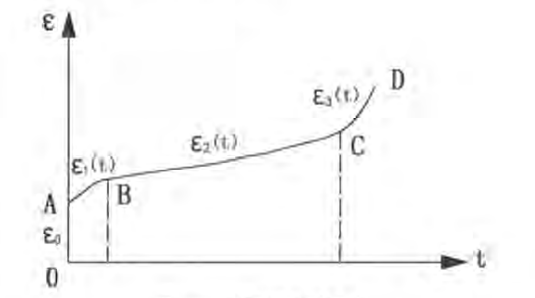
\includegraphics[width=0.5\textwidth]{img/chap3/蠕变曲线.png}
    \caption{蠕变曲线}
    \label{fig:3-1}

\end{figure}

由于岩石加速蠕变阶段变形规律复杂而且持续时间极为短暂,大多数经验模型都只是对岩石第一、第二阶段的蠕变变形进行描述,常见的蠕变经验公式如下:

1)幂函数型
\begin{equation}
     {\varepsilon}(t)=At^n
\end{equation}
式中,$A$、$n$是材料常数,其值与应力水平、材料特性和温度条件相关,多用于
反应减速蠕变阶段的性质。

2)对数型
\begin{equation}
     {\varepsilon}(t)={\varepsilon}_{0}+Blgt+Dt
\end{equation}
式中,$B$、$D$为与应力有关的常数,常用于反应加速蠕变阶段的性质。

3)指数型
\begin{equation}
     {\varepsilon}(t)=A[1-exp(f(t))]
\end{equation}
式中,$A$为材料常数、f(t)为时间f的函数,多用于反应等速蠕变阶段的性质。


上述经验流变本构模型是根据试验结果抽象得到的应力-应变—时间关系,不同的岩石,甚至相同岩石的不同试验都会得出不同的经验公式,因此必须在特定条件下才能得出相应的经验流变模型中。在建立模型时,主要运用以下三种蠕变技术理论:

(1)老化理论

老化理论的流变状态方程以应变、应力和时间之间的关系来表示:
\begin{equation}
     {\varepsilon}=f({\sigma},{t})
\end{equation}

根据维亚络夫在《土力学的流变原理》中介绍的老化理论,总应变被视作瞬时弹性应变和蠕变应变的和,假设瞬时弹性应变为$\varepsilon_0$,蠕变应变为$\varepsilon_c$,则应变方程可表示为:
\begin{equation}
     {\varepsilon}={\varepsilon_0}+{\varepsilon_c}
\end{equation}
假设取$\varepsilon_c$=$\frac{\sigma}{E}$,$\varepsilon_e$=$f(\sigma){\Phi}'(t)$,式(2.6)可得:
\begin{equation}
     {\varepsilon}={\varepsilon_0}+{\varepsilon_c}=\frac{\sigma}{E}+f(\sigma){\Phi}'(t)
\end{equation}
函数币${\Phi}'(t)$表征了变形的增长随时间而减缓,从本质上反映了材料特性随时间的变化即“老化”,老化理论适用于确定某个具体时刻的变形值,而不依赖于这一时刻前的受荷历史,即不研究变形的全过程。当应力历史较为复杂时并不适用。

(2)流动理论

流动理论的流变状态方程以应变速率、应力和时间之间的关系来表示,变形速率等于弹性变形速率加蠕变变形速率:
\begin{equation}
     {\dot{\varepsilon}}=f({\sigma},{t})={\dot{\varepsilon_0}}+{\dot{\varepsilon_c}}
\end{equation}
假设$\dot{\varepsilon_0}$=$\frac{1}{E}\frac{\mathrm{d} \sigma}{\mathrm{d} t}
$,$\dot{\varepsilon_c}$=$f(\sigma)\chi(t)$,
\begin{equation}
     {\dot{\varepsilon}}=\frac{1}{E}\frac{\mathrm{d} \sigma}{\mathrm{d} t}+f(\sigma)\chi(t)
\end{equation}
“流动理论”这一名称是根据这个理论的方程和粘滞流动方程相似而得到的。蠕变方程通过对式(2.9)进行求积分得方式获得。

(3)硬化理论

硬化理论建立的是以应变速率、应力和应变本身所构成的表达式:
\begin{equation}
     {\dot{\varepsilon}}=f({\sigma},{\varepsilon})=\frac{f(\sigma)}{\phi(\varepsilon)}
\end{equation}

从这个式子可看出应变速率随应变的增加而减小,物体仿佛硬化了,这个理论因此而得名。

\subsection{元件组合模型}
元件组合模型是考虑岩体种类、应力、温度、湿度、辐射等因素的影响,表现出的一系列与时间相关的力学响应。以三种基本元件——弹性元件、粘性元件及塑性元件以不同的形式串联或并联组合成为某种更复杂的模型,据此推导其本构方程来近似地建立所研究岩石的本构关系。而对于特定的影响条件,如温度、湿度等,则通过该使用不同特性的基本元件来表示。目前学者们提出的模型有很多种,现在常见的模型有Burgers模型、西原模型和H-K模型等。下面介绍几种基本元件及简单的组合模型。

1.基本元件的力学模型

(1)弹性元件
\begin{figure}[ht!]
    \centering
            \centering
            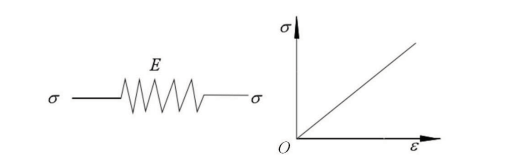
\includegraphics[width=0.6\textwidth]{img/chap3/Elastic element.png}
    \caption{弹性元件}
    \label{fig:3-2}
\end{figure}

弹性元件可以用弹簧表示,其应力-应变为线性关系,如图~\ref{fig:3-2},满足胡克定律,又称为胡克体(H),一维状态下的本构方程为:

\begin{equation}
{\sigma}={E}{\varepsilon}
\end{equation}

弹性元件的应力-应变关系不随时间变化,其应变是瞬时完成的,因此其不具有蠕变和松弛等流变特性。

(2)粘性元件
\begin{figure}[ht!]
    \centering
            \centering
            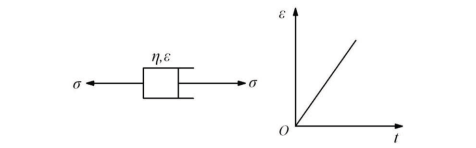
\includegraphics[width=0.6\textwidth]{img/chap3/Viscous element.png}
    \caption{粘性元件}
    \label{fig:3-3}
\end{figure}

粘性元件用于模拟材料的粘滞性,用粘壶表示,理想粘性体的应变与时间成线性关系,可称之为牛顿体(N),如图~\ref{fig:3-3}。可以认为粘壶是一个带孔的活塞在充满牛顿液体的圆筒
中运动。$\eta$为粘滞系数,表示应力与应变速率的比值,在一维状态下其本构方程为:

\begin{equation}
{\sigma}={\eta}\overset{\centerdot }{\mathop{\boldsymbol{\varepsilon}}}
\end{equation}

粘性元件在受力后不立即产生应变,应变随着时间的发展逐渐增大,具有流变特性。在受力过程中移去应力,应变不会恢复。

(3)塑性元件
\begin{figure}[ht!]
    \centering
            \centering
            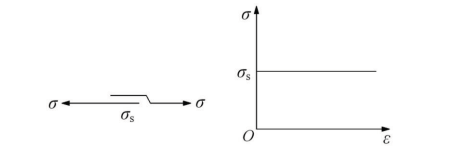
\includegraphics[width=0.6\textwidth]{img/chap3/Plastic element.png}
    \caption{塑性元件}
    \label{fig:3-4}
\end{figure}

塑性元件用于模拟材料的塑性,由一对接触面粗糙的滑块组成,如图~\ref{fig:3-4},又称圣维南塑性体(S),其在一维状态下其本构方程为:

\begin{equation}
    \left\{\begin{matrix}
               \varepsilon =0& \sigma <{{\sigma }_{s}} & \\
               \varepsilon \to \infty & \sigma \ge {{\sigma }_{s}}  &
    \end{matrix}\right.
\end{equation}

当塑性体应力小于材料的屈服极限时,塑性体表现出刚体的性质,不产生任何变形,而当其应力达到或超过屈服极限时,可产生任意应变值,并且即使应力不再增加,应变也会持续增长,一旦应力去除,应变增长停止而留下永久变形。

通过将以上三种基本元件进行串并联组合可以清晰地反映岩石的黏弹性、黏塑性和
黏弹塑性等流变性质。

2.组合模型

(1)Maxwell(马克斯威尔)模型

该模型时由一个弹性元件和一个粘性元件串联形成得粘弹性体。
\begin{figure}[ht!]
    \centering
            \centering
            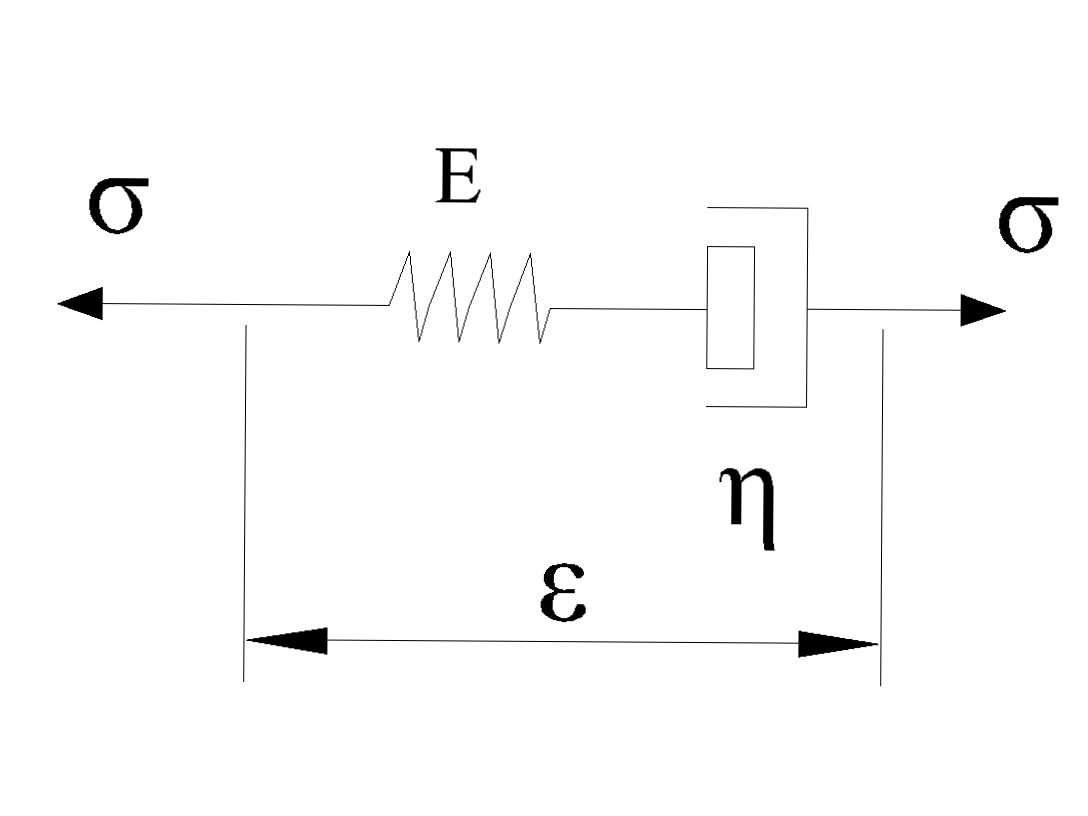
\includegraphics[width=0.4\textwidth]{img/chap3/Maxwell.png}
    \caption{Maxwell模型}
    \label{fig:3-5}
\end{figure}

由两个元件串联可得:
\begin{equation}
\left\{\begin{matrix}
          &\sigma ={{\sigma}_{1}}={{\sigma }_{2}}   \\
          &\boldsymbol{\varepsilon} ={{\boldsymbol{\varepsilon} }_{1}}+{{\boldsymbol{\varepsilon} }_{2}} 
         =\frac{{\sigma }_{1}}{E}+\frac{{\sigma }_{2}}{\eta}
        \end{matrix}  
 \right.
\end{equation}

由上式可模型本构方程为:
\begin{equation}
     \overset{\centerdot }{\mathop{\boldsymbol{\varepsilon} }}\,=\frac{1}{E}\overset{\centerdot }{\mathop{\sigma }}\,+\frac{1}{\eta }\overset{\centerdot }{\mathop{\sigma }}
\end{equation}

施加恒定应力$\sigma_0$,此时Maxwell模型的蠕变方程为:
\begin{equation}
     {\varepsilon}=\frac{\sigma_0}{E}+\frac{\sigma_0}{\eta }t
\end{equation}


2.Kelvin(开尔文)模型

该模型由一个弹性元件与一个粘性元件并联而成。
\begin{figure}[ht!]
    \centering
            \centering
            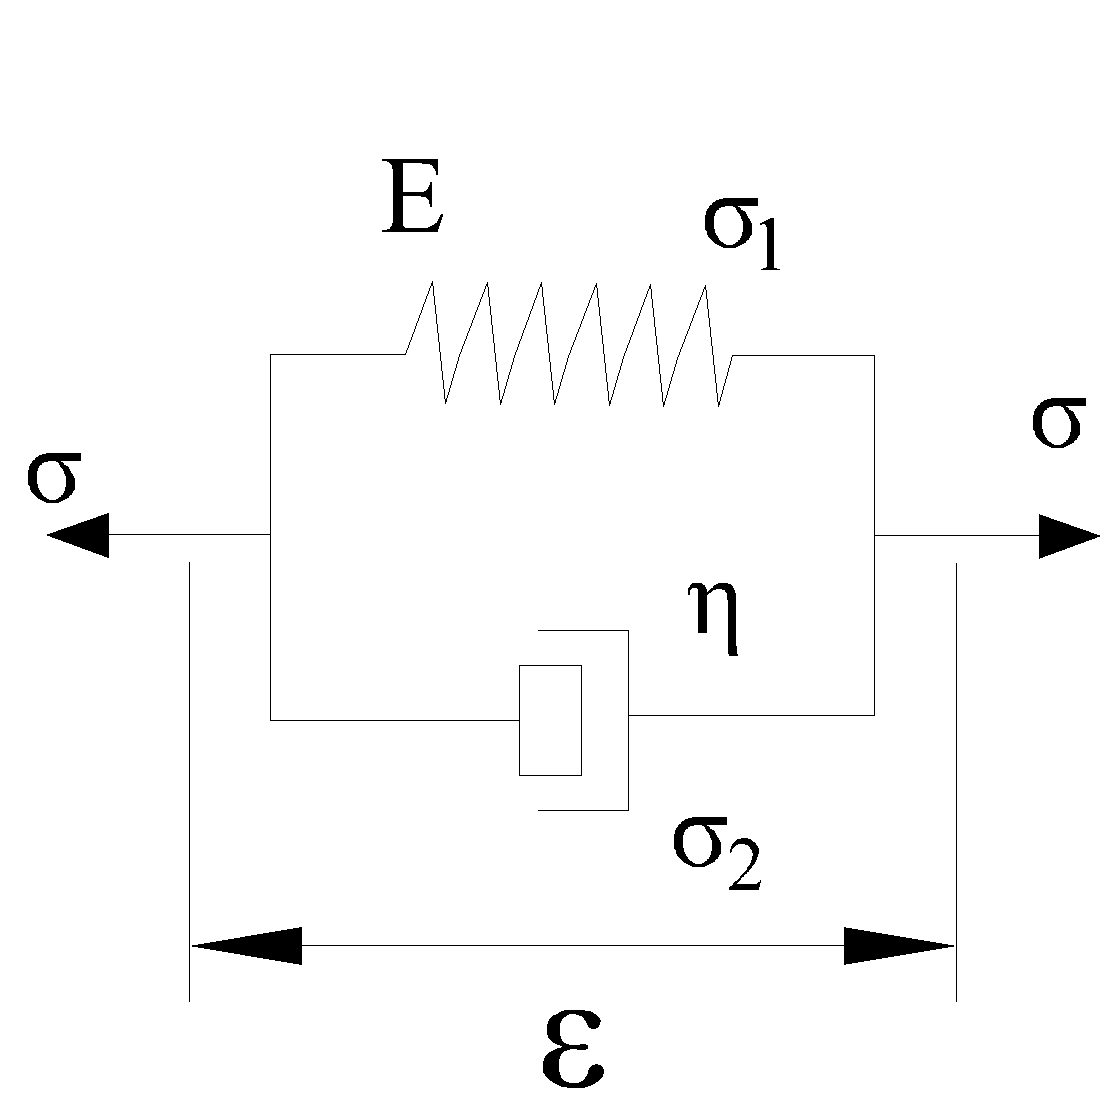
\includegraphics[width=0.4\textwidth]{img/chap3/Kelvin.png}
    \caption{Kelvin模型}
    \label{fig:3-6}
\end{figure}

由两个元件并联可得如下方程组:

\begin{equation}
  \left\{
  \begin{matrix}
 &\sigma =\sigma _1+\sigma _2  \\
 & \boldsymbol{\varepsilon} =\boldsymbol{\varepsilon}_1=\boldsymbol{\varepsilon}_2\\ 
 & \sigma _1=E \boldsymbol{\varepsilon}_1  \\
 & \sigma _2=\eta \dot{\boldsymbol{\varepsilon}_2}
 \end{matrix}
 \right.
\end{equation}

由式(3.11)可求得Kelvin模型得本构方程为:
\begin{equation}
\sigma=E\boldsymbol{\varepsilon}+\eta\dot{\boldsymbol{\varepsilon}}
\end{equation}

施加恒定应力$\sigma_0$,此时Kelvin模型的蠕变方程为:
\begin{equation}
     {\varepsilon}=\frac{\sigma_0}{E}(1-e^{-\frac{E}{\eta }t})
\end{equation}


3.粘塑性模型

该模型由一个粘性元件和一个塑性元件并联组成,用来模拟材料的粘塑性,如下图~\ref{fig:3-7}所示,用符号表示为V|N。粘塑性模型在应力加载时不产生弹性应变,因此在应力卸载后,模型发生的变形不能恢复。

\begin{figure}[ht!]
    \centering
            \centering
            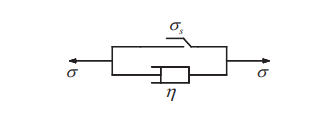
\includegraphics[width=0.4\textwidth]{img/chap3/V-N.png}
    \caption{粘塑性模型}
    \label{fig:3-7}
\end{figure}

当$\sigma$小于岩石材料屈服极限$\sigma_s$时,塑性元件不起作用,整体应变$\varepsilon$=0;当$\sigma$ $\geq$ $\sigma_s$时,塑性元件开始工作,模型产生粘塑性变形,由此可得该模型的本构方程为:

\begin{equation}
    \left\{\begin{matrix}
               \boldsymbol{\varepsilon} =0& \sigma <{{\sigma }_{s}} & \\
               \overset{\centerdot }{\mathop{\boldsymbol{\varepsilon} }}\,=\frac{\sigma -{{\sigma }_{s}}}{\eta } & \sigma \ge {{\sigma }_{s}}  &
    \end{matrix}\right.
\end{equation}

施加恒定应力$\sigma_0$后,该模型的蠕变方程为:
\begin{equation}
    \left\{\begin{matrix}
               \boldsymbol{\varepsilon} =0& \sigma <{{\sigma }_{s}} & \\
               {\varepsilon}=\frac{\sigma -{{\sigma }_{s}}}{\eta }t & \sigma \ge {{\sigma }_{s}}  &
    \end{matrix}\right.
\end{equation}

组合模型能够较好反应岩石流变各个阶段的变形特性,将基本元件相互组合可以得到具有粘弹、粘塑和粘弹塑性的本构模型。在一维状态下,目前较常用的线性流变组合模型如下表所示:
\begin{table}[ht!]\small
    \begin{tabular}{ccc}
    \toprule
        \makebox[0.1\textwidth][c]{模型名称} & \makebox[0.2\textwidth][c]{模型组成} & \makebox[0.4\textwidth][c]{本构方程}  \\
        \midrule
        \rule{0pt}{15pt}
        广义Kelvin模型        & H-(H|N)  &   \normalsize{$\sigma+\frac{\eta_1}{E_1+E_2}\dot{\sigma}=\frac{{E_1}{E_2}}{E_1+E_2}\varepsilon+\frac{{E_1}{\eta_1}}{E_1+E_2}\dot{\varepsilon}$}   \\ 
        \rule{0pt}{50pt}
        西原模型              & H-(H|N)-(S|N)  &  \normalsize{\makecell[c]{$\sigma \textless \sigma_s$,\\$\sigma+\frac{\eta_1}{E_1+E_2}\dot{\sigma}=\frac{{E_1}{E_2}}{E_1+E_2}\varepsilon+\frac{{E_1}{\eta_1}}{E_1+E_2}\dot{\varepsilon}$\\
        $\sigma \textgreater \sigma_s$,\\
        $(\sigma-\sigma_s)+(\frac{\eta_2}{E_1}+\frac{\eta_1+\eta_2}{E_2})\dot{\sigma}+\frac{\eta_1\eta_2}{E_1E_2}\ddot{\sigma}={\eta_2}{\dot{\varepsilon}}+\frac{\eta_1\eta_2}{E_1}\Ddot{\varepsilon}$}}\\
        \rule{0pt}{30pt}
        Burgers模型    &    H-N-(H|N)    &  \normalsize{$\sigma+(\frac{\eta_1}{E_1}+\frac{\eta_1+\eta_2}{E_2})\dot{\sigma}+\frac{\eta_1\eta_2}{E_1E_2}\ddot{\sigma}={\eta_1}{\dot{\varepsilon}}+\frac{\eta_1\eta_2}{E_2}\Ddot{\varepsilon}$}\\
        \rule{0pt}{30pt}
        广义Bingham模型  &   H-(N|S)  &  \normalsize{\makecell[c]{$\sigma \textless \sigma_s$,$\varepsilon=0$   \\
        $\sigma \textgreater \sigma_s$,$\dot{\varepsilon}=\frac{\dot{\sigma}}{E}+\frac{\sigma-\sigma_s}{\eta}$}}\\
    \bottomrule
        
    \end{tabular}
    \caption{常用组合模型及其本构方程}
    \label{tab:常用组合模型及其本构方程}
\end{table}

\section{岩石线性流变模型及参数拟合}
根据试验结果总结泥岩流变曲线的特征可以发现,在加载应力后会出现瞬时弹性变形,再之后会有随时间增长的流变变形,因此本构模型应该包含弹性元件和粘性元件。在进入稳定蠕变阶段后,蠕变速率减小到接近于0,因此可以用Kelvin模型来描述泥岩的衰减蠕变阶段。本文在这里选用经典Burgers模型来描述泥岩的线性流变力学特性。

burgers模型是由一个Maxwell体和一个Kelvin体串联构成的,具体形式如图所示:
\begin{figure}[ht!]
    \centering
            \centering
            \includegraphics[width=0.6\textwidth]{img/chap3/Burgers.png}
    \caption{Burgers模型}
    \label{fig:3-8}
\end{figure}
Burgers模型的总应力和总应变可以表示为:
\begin{equation}
    \left\{\begin{matrix}
               \sigma=\sigma_1=\sigma_2  \\
               \varepsilon = \varepsilon_1+\varepsilon_2\\
    \end{matrix}\right.
    \label{eq:3-22}
\end{equation}

\begin{figure}[ht!]
    \centering
            \centering
            \includegraphics[width=0.7\textwidth]{img/chap3/C-01.pdf}
    \caption{Burgers模型}
    \label{fig:3-9}
\end{figure}




由于Burgers模型是由Maxwell体和Kelvin体串联而成,根据他们的本构方程和串联元件的应力和应变关系(如式\ref{eq:3-22}),消去$\varepsilon_1$和$\varepsilon_2$,可以求得Burgers模型的本构方程为:
\begin{equation}
    \sigma+(\frac{\eta_1}{E_1}+\frac{\eta_1+\eta_2}{E_2})\dot{\sigma}+\frac{\eta_1\eta_2}{E_1E_2}\ddot{\sigma}={\eta_1}{\dot{\varepsilon}}+\frac{\eta_1\eta_2}{E_2}\Ddot{\varepsilon}
    \label{eq:3-23}
\end{equation}

在流变试验中,当荷载恒定时,令$\sigma=\sigma_0$,代入式\ref{eq:3-23}整理得到Burgers模型的流变方程为:
\begin{equation}
    \varepsilon(t)=\frac{\sigma_0}{E_1}[1-exp(-\frac{E_1}{\eta_1}t)]+\frac{\sigma_0}{E_2}+\frac{\sigma_0}{\eta_2}t
    \label{eq:3-23}
\end{equation}


\section{岩石非线性流变模型及参数拟合}
\subsection{泥岩非线性流变模型确定}
大量的试验研究结果表明,泥岩具有非线性流变特征,而这种特征在加速流变阶段最为明显,为了更确切地描述泥岩的流变特性,就要研究岩石的非线性流变问题,目前构建岩石非线性流变模型的方法有:

(1)基于实验结果,通过回归分析拟合经验方程,针对岩石流变的非线性问题,可以采用幂函数型的经验公式:
\begin{equation}
     {\dot\varepsilon}=A\sigma^nt^m
\end{equation}

$\dot\varepsilon$为流变速率,$\sigma$为加载应力水平,$t$为加载时间,A,n,m为与材料、应力、时间相关的参数,可以根据流变实验结果拟合得到。

(2)基于现有的线性流变模型,串联或并联一个非线性元件,构建一个可以描述流变加速阶段的流变本构模型。

(3)把线性元件组合模型中的线性元件替换为非线性元件,或将模型中的线性元件参数改为与材料、应力、时间相关的非常定参数方程,以此来研究岩石的非线性流变问题。

(4)结合内时理论、损伤断裂力学等理论等方法,在线性流变模型中引入损伤变量,达到构建非线性流变模型的目的。

本文拟采用第一种方法,利用试验数据对经验公式进行拟合得到泥岩的非线性本构模型。根据试验结果,泥岩流变过程受到时间、应力等因素的影响,再考虑到温度对工程中围岩流变的影响,本文拟采用根据Wallner、Hunsche和Schulze等基于错位理论,从盐岩细观结构层面提出的BGRa流变本构模型进行模拟研究\cite{1981Thermomechanical,Hunsche1999Rock},该模型是一种幂函数型的本构模型。他们认为盐岩是一种多晶材料,其蠕变行为在本质上是晶体错位运动的结果。岩盐的初始瞬态蠕变阶段仅持续时间较短。且初始蠕变量在总蠕变量中所占比例很小。因此在不考虑初始蠕变与加速蠕变阶段的情况下,可采用稳态蠕变模型研究长期变形,这也符合流变试验所得出的结论。

引入BGRa模型来描述泥岩稳态流变变形随温度和应力的函数关系:

\begin{equation}
    \dot{\boldsymbol{\varepsilon}}=A\mathrm{exp}\left ( -\frac{Q}{RT}\right ) \left (\frac{\sigma_1-\sigma_3}{\sigma^*}\right )^m
\end{equation}
\begin{shizhong}
    \item $A$、$n$\,---\,为材料参数;
    \item $Q$\,---\,为材料的有效激活能;
    \item $R$\,---\,为理想气体常数;
    \item $T$\,---\,试验温度;
\end{shizhong}

在BGRa模型中,将蠕变速率描述为:
\begin{equation}
    \begin{gathered}
        \dot { \boldsymbol{\varepsilon}}^\text{cr} ({ \boldsymbol{\sigma}})={\color{black} {\sqrt{\frac{3}{2}}}}Ae^{-Q/(RT)}\left(\dfrac{{\bar \sigma}}{\sigma_\text{ref}}\right)^m\dfrac{{\boldsymbol s}}{{\left\Vert{\boldsymbol s}\right\Vert}}
    \end{gathered}
\end{equation}

其中, ${ \bar\sigma}$ 为等效应力, ${ \bar\sigma}={\sqrt{{\frac{3}{2}}}}{\left\Vert{\boldsymbol s}\right\Vert}$ ,偏应力 ${\boldsymbol s}= { \boldsymbol{ \sigma}}-\frac{1}{3}{ \mathrm{tr}(\boldsymbol{\sigma}}){\mathbf I}$.

通过引入:
\begin{equation}
    b={\left(\dfrac{3}{2}\right)^{(m+1)/2}} \dfrac{Ae^{-Q/(RT)}}{\sigma_\text{ref}^m}
\end{equation}

即蠕变应变率可表示为:
\begin{equation}
    \begin{gathered}
        \dot { \boldsymbol{\varepsilon}}^\text{cr} ({ \sigma}) = b {\left\Vert{\boldsymbol s}\right\Vert}^{m-1} {\boldsymbol s}
    \end{gathered}
    \label{eq:bgra}
\end{equation}

最终,考虑蠕变和热应变的总应变率可表示为:
\begin{equation}
    \begin{gathered}
        \dot { \boldsymbol{\varepsilon} }= \dot { \boldsymbol{\varepsilon}}^\text{el} + \dot {\boldsymbol{\varepsilon}}^\text{th}
        + \dot { \boldsymbol{\varepsilon}}^\text{cr}
    \end{gathered}
\end{equation}
其中, $\dot {\boldsymbol{\varepsilon}}^\text{el}$ 是弹性应变率, $\dot { \boldsymbol{\varepsilon}}^\text{th}$ 是热应变率,  $\dot {\boldsymbol{\varepsilon}}^\text{cr}$是蠕变应变率。


\subsection{非线性流变模型参数辨识}
常见的参数识别方法有最小二乘法,最小二乘法的基本原理为根据n组试验数据$(X_k,Y_k)(k=1,2,3,\dots,n)$,应变量Y是自变量X和待求参数A的确定函数,$Y=f(X,A)$,其中自变量X和待求参数A可以有多个$(X=\{x_1,x_2,…,x_p\},A=\{a_1,a_2,…,a_q\})$。要求出参数$a$,就要使残差平方和Q达到最小值,必须满足如下条件:
\begin{equation}
    Q=\sum_{k=1}^n[Y_k-f(X_k,A)]^2
\end{equation}

\begin{equation}
    \frac{\partial{Q}}{\partial{a_i}}=0(i=1,2,\dots,q)
\end{equation}

Levenberg-Marquardt非线性优化最小二乘法,即$L-M$算法,是一种介于牛顿法和梯度下降法之间的非线性优化算法。对于过参数化的问题不敏感,能有效处理冗余参数的问题,使代价函数陷入局部极小值的机会大大
减小,这些特性使得$L-M$算法在各领域都得到广泛应用。L-M算法本质上是在迭代过
程中把原问题化为多个$LS$问题进行求解。其非线性关系的一般形式为:
\begin{equation}
    y=f(x,d)
\end{equation}

其中f为给定的非线性函数;$x=(x_1,x_2,\dots,x_m))$为自变量向量,$d=(d_1,d_2,\dots,d_n)$为未知参数向量,假设对x和y进行p次运算,得到p组数据X和Y,其残差平方和e为:
\begin{equation}
    e=\sum_{i=1}^p[Y_i-f(X_i,d)]^2
\end{equation}

$L-M$算法的目的是求出一组d使e极小化。若第k次迭代结果为$d^(k)$,则将f(X,d)在$d^(k)$附
近的一阶近似表示为:
\begin{equation}
    f(d^{(k)}+\delta^{(k)})\approx f(x,d^{(k)})+A^{(k)}\delta^{(k)}
\end{equation}

其中:
\begin{equation}
    A^{(k)}=[\frac{\partial{f(x,d)}}{\partial{d_j}}]_{d=d^{(k)}},j=1,2,\dots,n
\end{equation}

使得:
\begin{equation}
    {\left\Vert{\boldsymbol y-f(x,b^{(k+1)})}\right\Vert}=\mathop{\min}_{\delta^k}{\left\Vert{\boldsymbol A^{(k)}\delta^{(k)}-e^{(k)}}\right\Vert}
\end{equation}

也就是在己知$A^{(k)}$和$e^{(k)}$的情况下,解超定线性方程$A^{(k)}\delta^{(k)}=e^{(k)}$,其最小二乘解为:

\begin{equation}
    \label{eq:3-35}
    (\delta^{(k)})_{LS}=((A^{(k)})^{'}A^{(k)})^{-1}(A^{(k)})^{'}e^{(k)}
\end{equation}

而对于L-M算法,用$(A^{(k)})^{'}A^{(k)}+{\lambda_k}I$代替式\ref{eq:3-35}中的$(A^{(k)})^{'}A^{(k)}$,则有:

\begin{equation}
    (\delta^{(k)})_{LM}=((A^{(k)})^{'}A^{(k)}+{\lambda_k}I)^{-1}(A^{(k)})^{'}e^{(k)}
\end{equation}

其中:$\lambda_k$和${\lambda_k}I$分别称为阻尼因子和阻尼项,这使得L-M算法相较于最小二乘法,克服了系数矩阵奇异和病态时导致的异常情况。当$\lambda_k$=0时,即为高斯.牛顿法;当$\lambda_k$取值很大时,接近梯度下降法。由于$L-M$算法利用了近似的二阶导数信息,故比梯度下降法快得多。基于以上优点,
本文选择$L-M$算法进行参数拟合。

首先,我们需要考虑的是符合上一章所完成试验的具体情况——在进行流变试验时,未考虑温度因素的影响,所以对BGRa模型进行一定程度的修改:

\begin{equation}
    \dot{\boldsymbol{\varepsilon}}=A\Delta\sigma^m
    \label{eq:3-37}
\end{equation}

$\Delta\sigma$——试验过程中所施加的偏应力

根据泥岩室内流变试验得到的数据,采用Levenberg-Marquardt非线性优化最小二乘法对式\ref{eq:3-37}的位置参数A、m进行拟合。基于Origin软件的非线性曲线拟合功能,自定义拟合函数为变形后的BGRa流变方程。在本次曲线拟合中,我们需要确定的是加载应力水平对流变速率的影响关系,而BGRa模型是描述稳态蠕变阶段的本构模型,因此我们在选择拟合数据时,选择对应各级加载应力水平的稳态蠕变阶段的流变速率。

在拟合数据时,因为在C-03这一组试验中几乎不存在稳定蠕变阶段,试样在应力施加后很快就破坏了,所以单轴流变试验选取了除C-03以外的四组数据。而在三轴流变试验的三组数据中,选取了完整度比较高的D-02的分级加载试验数据,对每一级的应力及稳定蠕变速率的参数方程进行了数据拟合。计算出各试样的蠕变经验模型参数如表\ref{tab:单、三轴试验BGRa流变模型参数}所示,对应的拟合曲线如图\ref{fig:3-8}、\ref{fig:3-9}所示。

\begin{table}[ht!]\small
    \begin{tabular}{p{3cm}<{\centering} p{3cm}<{\centering} p{3cm}<{\centering} p{3cm}<{\centering}}
        \toprule
        试样编号  & $A$  &  $m$   & 拟合效果/$R^2$\\
        \midrule
           C     &   1.14791E-18   &    8.90542   &   0.976\\
        \midrule
        D-02    &   9.61511E-18   &    6.42455   &   0.992 \\
        \bottomrule
    \end{tabular}
    \caption{BGRa流变模型参数}
    \label{tab:单、三轴试验BGRa流变模型参数}
\end{table}

\begin{figure}[ht!]
    \centering
            \centering
            \includegraphics[width=0.6\textwidth]{img/chap3/Uniaxial curve fitting.png}
    \caption{单轴流变速率试验数据和拟合曲线}
    \label{fig:3-8}
\end{figure}

\begin{figure}[ht!]
    \centering
            \centering
            \includegraphics[width=0.6\textwidth]{img/chap3/Triaxial curve fitting.png}
    \caption{10MPa围压下流变速率试验数据和拟合曲线}
    \label{fig:3-9}
\end{figure}

由上述表中的数据和拟合曲线图可以看出,在单轴试验和三轴试验中,泥岩的稳态流变速率都随着加载应力等级的提升而增大。由图\ref{fig:3-8}和\ref{fig:3-9}可知,BGRa流变模型拟合曲线与蠕变试验结果总体吻合较好,但在应力较低的水平下拟合有所偏差。两条曲线拟合平均调整后的$R^2$分别为0.976和0.992,说明整体拟合的效果较好,而且对于三轴试验中的数据拟合效果更好。总体上来说,BGRa流变模型可以用来描述该泥岩的流变特性。

\section{小结}
本章对岩石的线性流变元件和基本流变本构模型进行了简单介绍,选取了xxx和BGRa等不同的本构模型来描述稳态蠕变阶段的泥岩的流变速率的特征,并对该流变方程进行了参数拟合,得到如下主要成果:

(1)经验型流变本构模型往往根据试验结果,不追求岩石的流变机理,通过数学函数抽象得到的应力、应变、时间关系,属积分型本构方程。在本章中简单介绍了常用的幂函数模型、指数模型、对数模型等经验模型,以及在建立模型时,主要运用的三种蠕变技术理论——老化理论、流动理论和硬化理论。

(2)通过介绍几种基本力学元件和简单的组合模型,例如Maxwell体、Kelvin体、粘塑性模型等,了解到元件组合模型的基本原理,能够将岩石在流变过程中的不同特性通过基本元件的力学性质表现出来。相比经验模型,元件组合模型更具有通用性,能够更好地反映岩石的实际流变特征。

(3)基于上一章的流变试验结果,根据泥岩在不同加载应力状态下的流变特性,计算其流变速率,选取BGRa模型来描述泥岩的流变本构关系。基于Origin软件,通过自定义的流变方程,利用试验数据拟合进行参数拟合,得到BGRa模型的相关参数。
%通过比较试验数据曲线和拟合曲线,发现BGRa流变模型可以较为准确地描述该泥岩的流变特性。







    \chapter{泥岩流变数值模拟研究}
岩土工程研究的核心问题即变形与稳定性评价。工程扰动造成边坡应力场及位移场发生变化,在流变作用下位移随时间有不同程度的发展。过大的变形将导致其上构筑物受力变形的改变,影响构筑物正常工作运营,甚至造成构筑物破坏。因此,对大型岩土工程项目,分析其岩土体变形发展趋势,对工程稳定性进行评价具有重要意义。





\section{数值模型}

取江苏金坛某一长轴为\SI{70}{m},短轴为\SI{30}{m}的椭球形溶腔为研究对象进行二维测试。根据王贵君\cite{王贵君2003盐岩层中天然气存储洞室围岩长期变形特征}的研究表明,模型宽度为腔\num{5}倍以上时候,边界效应对围岩的影响可忽略不计。因此取试算模型宽度为\SI{400}{m}。为提高计算效率,故取溶腔一半进行计算,模型简图如图~\ref{jiantu}~所示。对模型进行有限元计算单元网格划分,共划分\num{3202}个单元,\num{3325}个节点,如图~\ref{jiantu}~所示。


\begin{figure}[ht!]
    \centering
    \subfigure[二维模型简图]
    {
        \begin{minipage}{7cm}
            \centering
            \includegraphics[width=0.95\textwidth]{img/chap4/计算模型简图.pdf}
        \end{minipage}
    }
    \subfigure[二维模型网格划分图]
    {
        \begin{minipage}{7cm}
            \centering
            \includegraphics[width=0.95\textwidth]{img/chap4/2dmoxing.pdf}
        \end{minipage}
    }
    \caption{二维试算模型简图及网格图}
    \label{jiantu}
\end{figure}

\section{初始条件和边界条件}
计算模型的尺寸、边界等信息见图~\ref{jiantu}。

\begin{enumerate}
    \item 地应力
    
    根据马林建等\cite{马林建2009深部盐岩含夹层地层初始地应力场模拟分析}对深部盐岩自重应力分布的模拟计算结果,随着时间的增加,下底层侧压力系数不断增大,岩层越深增大的幅度越大,并趋近于$1$。本文中计算所取溶腔中心处于地下\SI{1000}{m}深处,取侧压系数$\lambda$=1,即地应力状态按照静水应力状态考虑。侧压系数$\lambda$指某点最大水平应力和垂直主应力的比值,或用两个水平应力的平均值与垂直应力的比值表示。
    %沿深度方向设置应力梯度,梯度大小为各岩层容重。

    \item 边界条件

    模型的上表面无应力边界条件;模型下表面用Y向简支约束,四周表面受相应法线方向上的简支约束,即认为模型左、右面及下端面以外的地质体为刚性体,不允许其产生法向移动,溶腔对它们的影响可以忽略。

    \item 温度条件

    模型顶端设置固定温度,为\SI{20}{\celsius} ,温度梯度为\SI{13}{\celsius/km},即围岩初始温度为\SI{33}{\celsius}。溶腔内初始压力为\SI{10}{MPa}。计算过程中温度和压力均保持不变。
\end{enumerate}

\section{模型参数}\label{section:modelparameters}
计算采用RGBa蠕变本构模型,根据金坛盐岩实验结果数据,选定相关参数如表\ref{tab:1}所示。盐岩基本力学参数及热工计算基本物理参数如表\ref{tab:2}-表\ref{tab:3}所示。

\begin{table}[ht!]\small
    \centering
    \begin{tabularx}{\textwidth}{C{1.0}C{1.0}C{1.0}C{1.0}C{1.0}}
        \toprule
        岩层 & A ($\rm{d^{-1}}$) & Q(kJ/mol) & R (kJ/mol) & m \\
        \midrule
        盐岩 & $1.336×10^{-6}$   & 15900     & 8.3143     & 5 \\ \bottomrule
    \end{tabularx}
    \caption{盐岩RGBa模型参数}
    \label{tab:1}
\end{table}

\begin{table}[ht!]\small
    \centering
    \begin{tabularx}{\textwidth}{C{1.0}C{1.0}C{1.0}C{1.0}}
        \toprule
        岩层 & 弹性模量(GPa) & 泊松比  & 密度($\rm{kg/m^3}$) \\
        \midrule
        盐岩 & 18        & 0.27 & 2310              \\
        \bottomrule
    \end{tabularx}
    \caption{盐岩基本力学参数}
    \label{tab:2}
\end{table}

\begin{table}[ht!]\small
    \centering
    \begin{tabularx}{\textwidth}{C{0.5}C{1.5}C{1.0}C{1.0}}
        \toprule
        岩层 & 导热系数($\rm{W/(m \cdot K}$)) & 比热($\rm{J/(kg\cdot K)}$) & {热膨胀系数($\rm{10^{-6}/K}$)}  \\
        \midrule
        盐岩 & 5.875         & 861                           & \num{1.2e-5} \\ \bottomrule
    \end{tabularx}
    \caption{盐岩热力学参数}%\todoiZN{热膨胀系数有单位吧}
    \label{tab:3} 
\end{table}

\section{二维模型验证}

\subsection{位移场分析}

当围岩温度分别为\SI{35}{\celsius}、\SI{90}{\celsius}、\SI{150}{\celsius}时,位移云图如~\ref{weiyiyuntu}~所示。位移在溶腔顶部和底部较小,主要集中于溶腔腰部。为分析岩体流变变形,移除最初卸荷产生的弹性形变后,绘制溶腔腰部流变最大值处位移与时间的变化关系曲线,见图~\ref{dispalment-t}。由图可知,岩体在\numrange{0}{20}天内处于初始蠕变阶段,蠕变速率较大,20天以后处于稳态蠕变阶段,蠕变速率趋于平缓。温度为\SI{35}{\celsius}时,位移最大值为\SI{0.044}{m};温度为\SI{90}{\celsius}时,位移最大值为\SI{0.047}{m};温度为\SI{150}{\celsius}时,位移最大值为\SI{0.050}{m}。由二维模型试算可得:(1)围岩温度越高产生流变越大;(2)腔体内缩,且位移主要集中于腔腰部分;(3)应力主要集中于腔顶和腔底。试算结果符合盐岩蠕变的温度效应规律和椭球型腔体的实际破坏情况。

\begin{figure}[ht!]
    \centering
    \includegraphics[width=0.55\textwidth]{img/chap4/不同温度(35℃、90℃、150℃)位移与时间曲线图.pdf}
    \caption{不同温度(35℃、90℃、150℃)位移与时间曲线图}
    \label{dispalment-t}
\end{figure}

\begin{figure}[ht!]
    \centering

    \subfigure[35℃位移云图]
    {
        \begin{minipage}{7cm}
            \centering
            \includegraphics[width=0.95\textwidth]{img/chap4/35weiyi.pdf}
        \end{minipage}
    }
    \subfigure[90℃位移云图]
    {
        \begin{minipage}{7cm}
            \centering
            \includegraphics[width=0.95\textwidth]{img/chap4/90weiyi.pdf}
        \end{minipage}
    }
    \subfigure[150℃位移云图]
    {
        \begin{minipage}{7cm}
            \centering
            \includegraphics[width=0.95\textwidth]{img/chap4/150weiyi.pdf}
        \end{minipage}
    }
    \caption{不同温度下位移云图(单位:m)}
    \label{weiyiyuntu}
\end{figure}




\subsection{应力场分析}

由图~\ref{fig:Mises}不同温度下的Mises应力云图可以看出,溶腔在卸载后应力会发生重分布,在腔体顶部和腔体底部会形发生力集中现象。当温度为\SI{35}{\celsius}、\SI{90}{\celsius}、\SI{150}{\celsius}时,最大Mises应力分别为\SI{4}{MPa}、\SI{3.4}{MPa}、\SI{3.0}{MPa}。温度越高,最大Mises应力越小。


\begin{figure}[ht!]
    \centering
    \subfigure[35℃~Mises应力云图]
    {
        \begin{minipage}{7cm}
            \centering
            \includegraphics[width=0.95\textwidth]{img/chap4/35mises.pdf}
        \end{minipage}
    }
    \subfigure[90℃~Mises应力云图]
    {
        \begin{minipage}{7cm}
            \centering
            \includegraphics[width=0.95\textwidth]{img/chap4/90mises.pdf}
        \end{minipage}
    }
    \subfigure[150℃~Mises应力云图]
    {
        \begin{minipage}{7cm}
            \centering
            \includegraphics[width=0.95\textwidth]{img/chap4/150mises.pdf}
        \end{minipage}
    }
    \caption{不同温度下Mises应力云图(单位:Pa)}
    \label{fig:Mises}
\end{figure}


\section{小结}

本章从地理位置、自然条件、地址条件等方面介绍了金坛盐矿的工程地质概况,重点阐述了金坛地区的盐岩层地质特征。并建立二维数值模型,编写OpenGeoSys计算脚本进行计算,得到了围岩的位移场、应力场随时间的变化情况。分析结果发现:(1)温度越高,围岩产生的最大位移越大;(2)盐岩储库呈现明显的初始蠕变和稳态蠕变特征;(3)围岩位移集中于腔腰,应力集中于腔顶和腔底。结论符合盐岩的力学特性、温度对盐岩蠕变影响规律,符合椭球形腔体的破坏特点,因此可校验计算方法和计算输入文件的合理性。
    \chapter{数值仿真结果与分析}


\section{模型描述}

本文选取江苏金坛盐矿某一溶腔进行模拟研究,将不规则溶腔模型简化为长轴为70m,短轴为30m的标准椭球体,理论储气约为26.4万方。溶腔中心点位于地下\SI{936.9}{m}处,溶腔顶部埋深\SI{901.9}{m},底部埋深\SI{971.9}{m},溶腔顶部盐岩厚165m,盐岩上部泥岩厚\SI{736.6}{m}。取地表温度为\SI{17}{ \degreeCelsius},温度梯度为\SI{2.24}{\degreeCelsius}/\SI{100}{m},则模型顶端温度(y=-901.9m)温度为\SI{37.1}{\degreeCelsius}(\SI{310.3}{K});模型下端(y=\SI{-971.9}{m})温度为\SI{38.7}{\degreeCelsius}(\SI{311.8}{K}),溶腔中心(y=\SI{-936.1}{m})温度为\SI{37.9}{\degreeCelsius}(\SI{311.0}{K})。

为消除边界对数值模拟的影响,土体模型尺寸应达到洞泾尺寸的\num{6}倍左右,因此建立长度为400m、宽度为400m、高为400m的轴对称模型。模型正视图如图\ref{fig:5-4}所示。模型底部采用位移边界条件,不论何种工况下底部沿水平方向或数值方向都不会发生位移,垂直方向两侧边界施加水平方向上的位移约束。盐岩计算所需参数见第\ref{section:modelparameters}节中表\ref{tab:1}-\ref{tab:3}。

为提高计算效率,将模型简化为1/4对称模型进行有限元计算,网格划分如图\ref{fig:5-4}所示,共计181935单元,193388节点。
 \begin{figure}[ht!]
    \centering
    \subfigure[三维模型示意图]
    {
        \begin{minipage}{8cm}
            \centering
            \includegraphics[width=0.85\textwidth]{img/chap5/计算模型图1.15.pdf}
        \end{minipage}
    }
    \subfigure[网格划分图]
    {
        \begin{minipage}{7cm}
            \centering
            \includegraphics[width=0.95\textwidth]{img/chap5/三维模型网格划分图.png}
        \end{minipage}
    }
    \caption{三维模型示意图与网格划分图}
    \label{fig:5-4}
\end{figure}


\section{注采方案}


\subsection{注采时长}
新能源储库的主要是为了调节峰谷时用电,缓解电网压力。电网负载一般由三大产业及居民用电构成,其中第一、第二产业处于全天生产状态,对于电网峰谷变化影响较小。电网的日负载波动主要是由于第三产业及居民日常活动引起。以江苏省为例,忽略季节性影响,民用电高峰时段一般是18时至23时共6小时,用电低谷期一般是1时至6时共计5小时\cite{谈康2016江苏电网负荷特性研究及有序用电管理措施探讨}。如下图\ref{fig:5-2}所示,为波兰2019年3月10日风力发电总量和电网荷载总量与时间关系图\cite{R2021Comprehensive}。图中黄色柱状图表示电网中荷载,蓝色柱状图表示风力发电总量,不难看出用电高峰时期风力发电能力较弱,而用电低谷时期风力发电能力较强。图中曲线表示除去风力发电所需电量,即全天电网荷载峰谷时波动曲线。

根据上述实际的用电情况的资料,制定储气库注采气运行工况如下:用电低谷期0时-7时匀速注气蓄能,用电高峰期7时至24时进行采气发电,以此为一个注采周期,依次循环\cite{谈康2016江苏电网负荷特性研究及有序用电管理措施探讨,R2021Comprehensive}。

\begin{figure}[ht!]
    \centering
    \includegraphics[width=0.95\textwidth]{img/chap5/波兰2019年某一天风力发电和电网总荷载与时间关系图.png}
    \caption{波兰一天内风力发电和电网总荷载与时间关系图\cite{R2021Comprehensive}}
    \label{fig:5-2}
\end{figure}


\subsection{内压变化}
盐岩地下储气库的稳定性包括两个方面,一是造腔施工期间的稳定性,二是保证储气库长期安全运行的稳定性。为保证储气库在设计年限内能安全运行,需对储气库的极限运行压力进行科学合理的设计。

(1)确定最小内压
最小内压的确定主要依据原则:一、顶板稳压原则;二、蠕变控制原则。顶板稳压原则:由于储气过程中腔内压力低于围岩地应力,造腔施工期间的弹性变形以及储库运行期间的蠕变变形会导致腔体顶板下沉。因此最小压力须满足防止顶板过度变形、开裂的变形约束要求。蠕变控制原则:储气库在长期运行的情况下岩石的蠕变会减小储库的有效容积,最小压力越大则一定年限内溶腔收缩率越小,因此最小运行压力须满足体积变化率的要求\cite{梁卫国2008层状盐岩储气库物理力学特性与极限运行压力}。

(2)确定最大内压
最大内压的确定主要依据原则:一、裸井致密原则;二、腔壁致密原则。裸井致密原则:裸井一般位于腔顶部岩层中,与套管靴相连,紧邻盖层,由于水泥与盐岩之间易发生变形不协调,导致气体泄漏。因此腔体内的最大气压必须有所限制,以此保证裸井的致密,避免气体泄漏。腔壁致密原则:
除了裸井之外,整个储库腔体内壁也应该保持致密,即内压应小于或等于最小地应力\cite{梁卫国2008层状盐岩储气库物理力学特性与极限运行压力}。

综合上述确定内压力原则,参考国内外实际储气库、储油库的建设经验,并考虑一定的安全系数,可以认为一般腔体内压的可行范围为上覆岩层压力的30$\%$-75$\%$\cite{王贞硕2020层状盐岩中水平腔压气蓄能储库顶板稳定性研究}。该溶腔上覆岩层压力为22.26MPa,理论允许运行压力范围为6.7MPa-16.7MPa。结合现实际储气库的运行状况的相关经验,拟定该储气库的运行压力上限为14MPa,运行压力下限为8MPa。

\subsection{温度变化}
根据热力学定律及理想气体方程,气体在压缩过程中会导致温度上升,并在注入腔体内后与围岩发生热量交换。图~\ref{fig:5-5}为韩中合参考Huntorf电站,对储气库系统模型求解结果\cite{韩中合2017储气室热力学特性对}。

如图(a)不同对流换热系数时储气室温度变化中显示,当对流换热系数h=0,即不考虑气体与围岩之间的热量交换时,初始气体温度为\SI{323}{K},注气阶段气体温度上升较快,近似呈线性变化,注气阶段结束后气体温度为\SI{378}{K};采气阶段气体温度也呈线性下降。直到采气阶段结束时,储气库压力恢复至初始气压,而气体温度略高于初始温度。随着$h$的增大,气体与围岩的热交换明显,气体温度上升和下降都逐渐缓慢。当h足够大时候,气体温度逐渐趋于平缓。当$h=\infty$,即恒温模型下,储气库运行各个阶段温度都保持不变,内压升高缓慢,系统运行时间最长。

参考该文献中储气库在运行过程中温度和压力随时间变化情况,制定本文中不考虑气体与围岩热量交换时储气库的运行工况。


\begin{figure}[ht!]
    \centering
    \subfigure[不同对流换热系数时储气室温度变化]
    {
        \begin{minipage}{7cm}
            \centering
            \includegraphics[width=0.95\textwidth]{img/chap5/不同对流换热系数时储气室温度变化.png}
        \end{minipage}
    }
    \subfigure[不同对流换热系数时储气室压力变化]
    {
        \begin{minipage}{7cm}
            \centering
            \includegraphics[width=0.95\textwidth]{img/chap5/不同对流换热系数时储气室压力变化.png}
        \end{minipage}
    }
    \caption{不同对流换热系数时储气室温度、压力变化\cite{韩中合2017储气室热力学特性对}}
    \label{fig:5-5}
\end{figure}


\section{新能源储库运行工况设置}
\subsection{考虑热力耦合}
综合上述注采周期、内压变化、注采温度变化分析,并结合江苏金坛地区已建储库的实际运作模式,拟定如图~\ref{fig:5-1}的新能源储库运行工况,以24小时为一个注采周期,\numrange{0}{7}小时注气,\numrange{7}{24}小时采气,如此循环往复。储库运行压力上限设定为\SI{14}{MPa},下限设定为\SI{8}{MPa}。计算得到气体最高温度为\SI{378}{K},最低温度为\SI{323}{K}。

\begin{figure}[ht!]
    \centering
    \includegraphics[width=0.55\textwidth]{img/chap5/储气库模拟运行工况.pdf}
    \caption{新能源储库考虑耦合模拟运行工况}
    \label{fig:5-1}
\end{figure}

% 实现计算脚本中储库运行工况设置如下。
% \begin{lstlisting}[breaklines,language=XML]
% <parameter>
%         <name>internal_pressure_value</name>
%         <type>Function</type>
%         <expression>(t%1>7.0/24.0? 144.0e6/17*(t%1)-280/17: -144.0e6/7*(t%1)-8.0e6)</expression>
% </parameter>
% <parameter>
%         <name>internal_bc_value</name>
%         <type>Function</type>
%         <expression>(t%1>7.0/24.0? -1320.0/17*(t%1)+6811/17: 1320.0/7*(t%1)+323)</expression>
% </parameter>
% \end{lstlisting}
% 其中internal\_pressure\_value为压力变化,压力单位为Pa,internal\_bc\_value为温度变化,温度单位为\si{K},时间$t$单位为\si{d}。

\subsection{不考虑热力耦合}
不考虑热力耦合的情况下,模拟新能源储库运行工况如图~\ref{fig:5-16}所示。周期压力的设置与考虑热力耦合的情况相同,参照前文对模型条件的描述,气体温度与溶腔中心温度相同,拟定为\SI{323.0}{K},且认为在气体压缩和释放过程中不发生温度变化。

\begin{figure}[ht!]
    \centering
    \includegraphics[width=0.55\textwidth]{img/chap5/压气蓄能库运行工况无耦合.pdf}
    \caption{新能源储库无耦合模拟运行工况}
    \label{fig:5-16}
\end{figure}

% 根据拟定的运行工况,计算代码中边界条件设置如下。
% \begin{lstlisting}[breaklines,language=XML]

% <parameter>
%     <name>internal_pressure_value</name>
%     <type>Function</type>
%     <expression>(t%1>7.0/24.0? 144.0e6/17*(t%1)-280e6/17: -144.0e6/7*(t%1)-8.0e6)</expression>
% </parameter>
% <parameter>
%     <name>internal_bc_value</name>
%     <type>Constant</type>
% <value>323.0</value>
% </parameter>
% \end{lstlisting}

\section{传统能源储库运行工况设置}

\subsection{考虑热力耦合}
利用地下盐穴作为传统能源储库(如:天然气储库),能够有效的保证供需平衡,维持供给的可靠性、连续性,避免出现供给不均匀的情况。因此相较于新能源储库,传统能源储库的循环注采周期较长,参考谭贤君等\cite{陈卫忠2007盐岩非线性蠕变损伤本构模型及其工程应用,盐岩储气库温度}在盐岩储气库温度-渗流-应力-损伤耦合模型研究、陈卫忠等在盐岩非线性蠕变损伤本构模型及其工程应用中的模型设置,并结合江苏金坛地区的天然气使用情况拟定储库运行工况。一年中,0-3月份为恒定低压阶段,0-6月份为注气阶段,6-9月份为恒定高压阶段,9-12月份为采气阶段。腔内气体最高压力为\SI{14}{Mpa},最低压力为\SI{8}{Mpa},最高温度为\SI{378}{K},最低温度为\SI{323}{K}。具体运行工况如图~\ref{fig:5_10}所示,以一年为一个循环周期,运行时间为10年进行模拟计算。
\begin{figure}[ht!]
    \centering
    \includegraphics[width=0.55\textwidth]{img/chap5/10年天然气储库运行工况.pdf}
    \caption{传统能源储库考虑耦合模拟运行工况}
    \label{fig:5_10}
\end{figure}
\begin{figure}[ht!]
    \centering
    \includegraphics[width=0.55\textwidth]{img/chap5/储气库无耦合.pdf}
    \caption{传统能源储库无耦合模拟运行工况}
    \label{fig:5_11}
\end{figure}
% 根据拟定的天然气储库实际运行工况,计算代码中循环边界条件设置如下。
% \begin{lstlisting}[breaklines,language=XML]
% <parameter>
%     <name>internal_pressure_value</name>
%     <type>Function</type>
%     <expression>(t%360>180? (t%360>270? 1.0e6/15*(t%360)-32.0e6: -14.0e6):(t%360>90? -1.0e6/15*(t%360)-2.0e6: -8.0e6))</expression>
% </parameter>
% <parameter>
%     <name>internal_bc_value</name>
%     <type>Function</type>
%     <expression>(t%360>180? (t%360>270? -11/18*(t%360)+543: 378):(t%360>90? 11/18*(t%360)+268: 323))</expression>
% </parameter>
% \end{lstlisting}


\subsection{不考虑热力耦合}
不考虑热力耦合的情况下,模拟实际储库运行进行计算。周期压力的设置与考虑热力耦合的情况相同,参照前文对模型条件的描述,气体温度与溶腔中心温度相同,拟定为\SI{311.0}{K},且认为在气体压缩和释放过程中不发生温度变化和热量交换。实际运行过程中,气体压力和温度的变化如图~\ref{fig:5_11}所示。



% 根据拟定的天然气储库实际运行工况,计算代码中循环边界条件设置如下。

% \begin{lstlisting}[breaklines,language=XML]
% <parameter>
%     <name>internal_pressure_value</name>
%     <type>Function</type>
%     <expression>(t%360>180? (t%360>270? 1.0e6/15*(t%360)-32.0e6: -14.0e6):(t%360>90? -1.0e6/15*(t%360)-2.0e6: -8.0e6))</expression>
% </parameter>
% <parameter>
%     <name>internal_bc_value</name>
%     <type>Constant</type>
%     <value>311.0</value>
% </parameter>
% \end{lstlisting}

\section{计算工况汇总}
从上述两种储库实际工况的分析中可以看出,新能源储库和传统能源储库工作时压力范围、温度范围大致相同,而循环周期差异较大。因此在长期模拟过程中,拟定两种储库的压力变化范围和温度变化范围不同,设置不同循环周期,以此比较两者长期运行过程中的稳定性。拟定工况汇总于表\ref{tab:5_10}。

\begin{table}[ht!]\small
    \centering
    \begin{tabular}{M{0.1\textwidth}M{0.1\textwidth}M{0.1\textwidth}M{0.06\textwidth}M{0.1\textwidth}M{0.1\textwidth}M{0.1\textwidth}M{0.1\textwidth}}
        \toprule
        计算工况 &储库类型&热力耦合 & 循环周期(d)& 最低内压 (MPa) & 最高内压(MPa) &最低温度 (K) & 最高温度(K) \\
        \midrule
        工况一 &新能源储库  &是  &1   &8    &14    & 323     & 378   \\
        \midrule
        工况二  &新能源储库   &否 &1   &8   &14    & 323     & 323  \\ 
         \midrule
        工况三  &传统能源储库   &是 &360  &8   &14    & 323  & 378  \\ 
         \midrule
        工况四 &传统能源储库   &否 &360  &8   &14    & 323    & 323  \\ \bottomrule
    \end{tabular}
    \caption{计算工况表}
    \label{tab:5_10}
\end{table}


\section{模型验证}
\subsection{模拟储库运营2天计算校验}

由于模型算量大,计算机算力有限,因此实际计算前,先进行代码可行性与合理性验证。将盐岩蠕变本构设置为弹性模型,进行运行测试。经理论分析,若围岩变形符合胡克定律,在周期荷载的作用下,则位移会产生周期性变化,且位移变化周期与荷载变化周期相同。

% 测试过程本构模型、参数修改代码如下。

% \begin{lstlisting}[language=XML]
% <constitutive_relation>
%     <type>LinearElasticIsotropic</type>
%     <youngs_modulus>E</youngs_modulus>
%     <poissons_ratio>nu</poissons_ratio>
% </constitutive_relation>
% \end{lstlisting}

% \begin{lstlisting}[language=XML]
% <parameter>
%     <name>E</name>
%     <type>Constant</type>
%     <value>18.0e9</value>
% </parameter>
% <parameter>
%     <name>nu</name>
%     <type>Constant</type>
%     <value>0.27</value>
% </parameter>
% \end{lstlisting}
% 测试采用弹性模型完成,其中E为杨氏模量,nu为泊松比,取值参照表\ref{tab:2}。

按照上述弹性本构模型试算文件进行计算,得到试算结果。取腔体围岩典型部位的三个点,绘制位移与时间的关系曲线如图~\ref{fig:E}所示。围岩位移随时间发生周期性变化且周期为\SI{1}{d},与边界条件的变化周期相同。可验证循环注采边界代码可行,且运行结果符合理论分析,可以对实际工程进行模拟计算。
\begin{figure}[ht!]
    \centering
    \includegraphics[width=0.55\textwidth]{img/chap5/弹性本构测试结果.pdf}
    \caption{弹性本构模型位移与时间关系曲线}
    \label{fig:E}
\end{figure}

\subsection{模拟储库运营7天结果分析}

\subsubsection{位移}
围岩位移云图如图~\ref{fig:dispalcement}所示,图~\ref{fig:dispalcement1d}为运行\SI{1}{d}后位移云图,图~\ref{fig:dispalcement7d}为运行\SI{7}{d}后位移云图。\SI{1}{d}与\SI{7}{d}整体蠕变趋势相同,腔顶下沉,腔底鼓起,腰部向内收缩。周围岩石因受到地应力的作用而向腔体内部收缩,主要集中于腔体腰部。由于地应力的不断增大,越接近腔底储库内压力与地应力差值越大,因此产生的位移越大。

\begin{figure}[ht!]
    \centering
    \subfigure[运行\SI{1}{d}围岩位移云图]
    {
        \begin{minipage}{7cm}
            \centering
            \includegraphics[width=0.95\textwidth]{img/chap5/1d位移云图.png}
        \end{minipage}
        \label{fig:dispalcement1d}
    }
    \subfigure[运行\SI{7}{d}围岩位移云图]
    {
        \begin{minipage}{7cm}
            \centering
            \includegraphics[width=0.95\textwidth]{img/chap5/7d位移云图.png}
        \end{minipage}
        \label{fig:dispalcement7d}
    }
    \caption{\SI{1}{d}、\SI{7}{d}围岩位移云图(单位:m)}
    \label{fig:dispalcement}
\end{figure}

腔体底部最大位移为\SI{0.174}{m},腔体顶部最大位移为\SI{0.123}{m}。由于腔体呈椭球状,在顶部和底部逐渐收缩,水平方向的应力逐渐相互抵消,因此产生的位移量小于腔体中部。水平应力的相互作用,也会导致围岩挤压而向内收缩,因此应力更大的腔底比腔顶位移大。

图~\ref{fig:7d_displacement_max}为\SI{7}{d}内最大位移与随时间变化情况。经过一个注采周期,即运行\SI{1}{d}后最大位移为\SI{0.097}{m},运行\SI{7}{d}后,最大位移为\SI{0.219}{m}。\SI{7}{d}内最大位移与时间变现出良好的线性关系,根据曲线规律,随着储库运行时间的增加,位移仍会大幅增加。


\begin{figure}[ht!]
    \centering
    \includegraphics[width=0.55\textwidth]{img/chap5/7d最大位移.pdf}
    \caption{\SI{7}{d}模拟运行最大位移与时间关系曲线}
    \label{fig:7d_displacement_max}
\end{figure}


在腔体上部、中部、下部取三个点,如图~\ref{fig:weizhi}所示,分别作出这三个点位移随着时间变化关系如图~\ref{fig:7d_displacement_A}所示。图像显示,在洞内压力周期性变化时,位移也成周期性变化,且变化周期与压力变化周期一致。

\begin{figure}[ht!]
    \centering
    \includegraphics[width=0.5\textwidth]{img/chap5/三点位移.png}
    \caption{A点、B点、C点位置}
    \label{fig:weizhi}
\end{figure}


\begin{figure}[ht!]
    \centering
    \includegraphics[width=0.55\textwidth]{img/chap5/三点位移随时间变化曲线.pdf}
    \caption{\SI{7}{d}内A点、B点、C点位移随时间变化曲线}
    \label{fig:7d_displacement_A}
\end{figure}

\subsubsection{应力}
围岩应力云图如图~\ref{fig:sigma}所示,图~\ref{fig:sigma1d}为运行\SI{1}{d}后应力云图,图~\ref{fig:sigma7d}为运行\SI{7}{d}后应力云图。应力集中于腔腰部位,运行\SI{7}{d}后,腔腰部最大应力可达\SI{164.9}{MPa},腔顶和腔底部分最大应力则相对较小,在\SI{20}{MPa}-\SI{50}{MPa}之间。
\begin{figure}[ht!]
    \centering

    \subfigure[运行\SI{1}{d}围岩应力云图]
    {
        \begin{minipage}{7cm}
            \centering
            \includegraphics[width=0.95\textwidth]{img/chap5/1d应力云图.png}
        \end{minipage}
        \label{fig:sigma1d}
    }
    \subfigure[运行\SI{7}{d}围岩应力云图]
    {
        \begin{minipage}{7cm}
            \centering
            \includegraphics[width=0.95\textwidth]{img/chap5/7d应力云图.png}
        \end{minipage}
        \label{fig:sigma7d}
    }
    \caption{运行\SI{1}{d}、\SI{7}{d}后围岩应力云图(单位:Pa)}
    \label{fig:sigma}
\end{figure}

围岩Von Mises应力云图如图~\ref{fig:Mises}所示。从图中可以看出,溶腔四周的Mises应力值都比较大,随着运行时间的增加,围岩内部会产生裂隙,裂隙扩张导致侧壁开裂破坏。并在溶腔的底部和顶部都有不同程度的应力集中,会导致腔顶岩层塌落,溶腔底部鼓胀开裂,这也与流变结果相符。通过比较运行\SI{1}{d}Mises应力与运行\SI{7}{d}Mises应力发现,\SI{7}{d}Mises应力值小于\SI{1}{d}Mises应力值,这是由于盐岩在蠕变过程中发生了应力重分布,其良好的蠕变特性延长了储库的使用寿命。
\begin{figure}[ht!]
    \centering

    \subfigure[运行\SI{1}{d}围岩应力云图]
    {
        \begin{minipage}{7cm}
            \centering
            \includegraphics[width=0.95\textwidth]{img/chap5/1dMises应力云图.png}
        \end{minipage}
        \label{fig:Mises1d}
    }
    \subfigure[运行\SI{7}{d}围岩应力云图]
    {
        \begin{minipage}{7cm}
            \centering
            \includegraphics[width=0.95\textwidth]{img/chap5/7dMises应力云图.png}
        \end{minipage}
        \label{fig:Mises7d}
    }
    \caption{运行\SI{1}{d}、\SI{7}{d}后围岩Von Mises应力云图(单位:Pa)}
    \label{fig:Mises}
\end{figure}

\begin{figure}[ht!]
    \centering

    \subfigure[运行\SI{1}{d}围岩温度云图]
    {
        \begin{minipage}{7cm}
            \centering
            \includegraphics[width=0.95\textwidth]{img/chap5/1d温度云图.png}
        \end{minipage}
        \label{fig:temperature1d}
    }
    \subfigure[运行\SI{7}{d}围岩温度云图]
    {
        \begin{minipage}{7cm}
            \centering
            \includegraphics[width=0.95\textwidth]{img/chap5/7d温度云图.png}
        \end{minipage}
        \label{fig:temperature7d}
    }
    \caption{\SI{1}{d}、\SI{7}{d}围岩温度云图(单位:K)}
    \label{fig:temperature}
\end{figure}

\subsubsection{温度}
围岩温度云图如图~\ref{fig:temperature}所示,图~\ref{fig:temperature1d}为运行\SI{1}{d}后温度云图,图~\ref{fig:temperature7d}为运行\SI{7}{d}后温度云图。围岩初始温度为\SI{298}{K},储库运行时气体温度最高为\SI{378}{K},最低为\SI{323}{K},由于温差气体与围岩会发生热交换,导致围岩温度上升。由图可以看出,围岩温度随着与溶腔的距离发生均匀变化。且温度影响范围并不大,运行\SI{1}{d}后,温度影响范围在在\SI{1.5}{m}以内;运行\SI{7}{d}后,温度影响范围在\SI{2.5}{m}以内,可见图~\ref{fig:temperaturefanwei}。

\begin{figure}[ht!]
    \centering
    \subfigure[运行\SI{1}{d}围岩温度变化范围]
    {
        \begin{minipage}{7cm}
            \centering
            \includegraphics[width=0.95\textwidth]{img/chap5/1d温度影响范围.png}
        \end{minipage}
       
    }
    \subfigure[运行\SI{7}{d}围岩温度影响范围]
    {
        \begin{minipage}{7cm}
            \centering
            \includegraphics[width=0.95\textwidth]{img/chap5/7d温度影响范围.png}
        \end{minipage}
       
    }
    \caption{\SI{1}{d}、\SI{7}{d}围岩温度影响范围(单位:K)}
    \label{fig:temperaturefanwei}
\end{figure}

运行\SI{7}{d}结束后,围岩最高温度为\SI{334.29}{K},但在每个周期运行约\SI{0.3}{d}后温度达到最大值,为\SI{377.35}{K}。由于腔体内气体温度呈周期性变化,因此围岩的温度在每个周期的前\SI{0.3}{d}随着气体温度迅速升高,在\SI{0.3}{d}达到温度最大值,随后溶腔附近的高温围岩向低温围岩传热,温度下降,并不会造成热量的大量累积。

\begin{figure}[ht!]
    \centering
    \includegraphics[width=0.55\textwidth]{img/chap5/7d最大温度.pdf}
    \caption{\SI{7}{d}内围岩最大温度与时间变化曲线}
    \label{fig:7d_temperature_t}
\end{figure}

围岩最高温度随时间变化的关系曲线如图所示~\ref{fig:7d_temperature_t}。由该曲线图可以看出,围岩温度在第一个周期内快速上升,自第一个周期以后在\SI{323}{K}-\SI{377.35}{K}之间作周期变化,达到\SI{377.35}{K}后不在上升,而是不断将热量传递至周围低温岩石,扩大温度影响范围。



\section{计算效率分析}
通过对该三维问题的并行计算处理,将原模型划分成多个子模型,借助超级计算机的不同处理器对多个子模型同时求解,可有效提高计算速度和处理能力。但因为非线性边界条件的存在,能够收敛的步长较小,目前计算步长取\SI{0.001}{d},计算模拟\SI{7}{d}运行一共需7000步。利用无锡超算中心商用平台计算,运行完7天共耗时\SI{75}{h},约为\SI{3.2}{d}。因三维问题求解时间过长,不满足计算的高效性原则,在不严重影响计算精度和计算规律,且保持长期循环温度、荷载不变的条件下改为二维计算。

二维计算模型较小,分割的计算单元少,利用超级计算机进行计算并不能有效提高计算效率,因此,尝试利用单一处理器性能力更强的个人计算机进行模拟。二维模型计算过程中,偏应力比三维中的大,非线性程度较高,步长取与三维中相同的\SI{0.001}{d}无法收敛,因此取\SI{0.0001}{d}进行计算。模拟\SI{7}{d}运行一共需70000步,运行完成共耗时\SI{0.12}{h}。当计算总时长为10年,预计需\SI{60.8}{h},即约\SI{2.5}{d}。求解时间大幅缩短,满足计算高效性原则。

综合上述试算结果及计算效率分析,维持原边界条件不变的情况下,将原三维模型转化为二维模型进行模拟试验。二维模型示意图、二维模型网格划分如图~\ref{fig:2dmodel}所示,共3202单元,3325节点。边界条件见。模型参数见第~\ref{section:modelparameters}节中表~\ref{tab:1}-\ref{tab:3}。

\begin{figure}[ht!]
    \centering
    \subfigure[二维模型简图]
    {
        \begin{minipage}{7cm}
            \centering
            \includegraphics[width=1.0\textwidth]{img/chap5/二维模型.pdf}
        \end{minipage}
    }
    \subfigure[二维模型网格划分图]
    {
        \begin{minipage}{7cm}
            \centering
            \includegraphics[width=0.95\textwidth]{img/chap5/二维网格.pdf}
        \end{minipage}
    }
    \caption{二维模型简图及网格图}
   %\todoiZN{左边的图的白边可以裁一下。}
    \label{fig:2dmodel}
\end{figure}

\section{新能源储库和传统能源储备库计算结果对比分析}

\subsection{位移分析}

上述不同工况下,储库运行十年后,位移云图如图~\ref{fig:4weiyi}所示。从云图中可以看出,腔体顶部下沉,底部鼓起,腰部向内收缩,且主要集中于腰部。周围岩石因受到的地应力的值大于腔体内气体压力,而产生向内收缩的位移。

\begin{figure}[ht!]
    \centering
    \subfigure[工况一运行\SI{10}{a}后位移云图]
    {
        \begin{minipage}{6.2cm}
            \centering
            \includegraphics[width=0.95\textwidth]{img/chap5/位移/工况一位移云图.pdf}
        \end{minipage}
    }
    \subfigure[工况二运行\SI{10}{a}后位移云图]
    {
        \begin{minipage}{6.2cm}
            \centering
            \includegraphics[width=0.95\textwidth]{img/chap5/位移/工况二位移云图.pdf}
        \end{minipage}
    }
    \subfigure[工况三运行\SI{10}{a}后位移云图]
    {
        \begin{minipage}{6.2cm}
            \centering
            \includegraphics[width=0.95\textwidth]{img/chap5/位移/工况三位移云图.pdf}
        \end{minipage}
    }
    \subfigure[工况四运行\SI{10}{a}后位移云图]
    {
        \begin{minipage}{6.2cm}
            \centering
            \includegraphics[width=0.95\textwidth]{img/chap5/位移/工况四位移云图.pdf}
        \end{minipage}
    }
    \caption{不同工况下运行十年后位移云图(单位:\si{m})}
    \label{fig:4weiyi}
\end{figure}



如图~\ref{fig:5_34}所示,在腔体围岩的腔顶、腔腰、腔底取A、B、C三个典型位置进行分析。图~\ref{fig:5_20}为不同工况下A、B、C三点位移与时间关系曲线。从图中可以看出,腰部位移最大,其次是底部,顶部位移最小。这是由于腔体呈椭球状,在顶部和底部逐渐收缩,水平方向的应力逐渐相互抵消,因此产生的位移量小于腔体中部。水平应力的相互作用,也会导致围岩挤压而向内收缩,因此应力更大的腔底比腔顶位移大。



\begin{figure}[ht!]
    \centering
    \includegraphics[width=0.6\textwidth]{img/chap5/应力/位置图.png}
    \caption{A、B、C三点位置图}
    \label{fig:5_34}
\end{figure}

\begin{figure}[ht!]
    \centering
    \subfigure[工况一典型位置位移与时间关系曲线]
    {
        \begin{minipage}{7cm}
            \centering
            \includegraphics[width=0.95\textwidth]{img/chap5/工况一顶部腰部底部位移与时间关系.pdf}
        \end{minipage}
    }
    \subfigure[工况二典型位置位移与时间关系曲线]
    {
        \begin{minipage}{7cm}
            \centering
            \includegraphics[width=0.95\textwidth]{img/chap5/位移/工况二顶部腰部底部位移与时间关系.pdf}
        \end{minipage}
    }
    \subfigure[工况三典型位置位移与时间关系曲线]
    {
        \begin{minipage}{7cm}
            \centering
            \includegraphics[width=0.95\textwidth]{img/chap5/位移/工况三顶部腰部底部位移与时间关系.pdf}
        \end{minipage}
    }
    \subfigure[工况四典型位置位移与时间关系曲线]
    {
        \begin{minipage}{7cm}
            \centering
            \includegraphics[width=0.95\textwidth]{img/chap5/位移/工况四顶部腰部底部位移与时间关系.pdf}
        \end{minipage}
    }
    \caption{不同工况下典型位置位移与时间关系曲线}
    \label{fig:5_20}
\end{figure}


新能源储库和传统能源储备库的最大位移与时间的关系曲线如图~\ref{fig:5_12}和图~\ref{fig:5_13}所示。计算结果显示,位移随着腔体内压的变化也呈现出周期性增大的趋势。运行的第一年内,位移快速增长,第一年之后位移增加速率变缓,总体成长趋势与运行时间呈现出良好的稳态流变效应。

\begin{figure}[ht!]
    \centering
    \includegraphics[width=0.55\textwidth]{img/chap5/位移/新能源储库10年最大位移与时间关系.pdf}
    \caption{新能源储库运行\SI{10}{a}后围岩最大位移与时间关系曲线}
    \label{fig:5_12}
\end{figure}

\begin{figure}[ht!]
    \centering
    \includegraphics[width=0.55\textwidth]{img/chap5/位移/传统能源储库10年最大位移与时间的关系.pdf}
    \caption{传统能源储库运行\SI{10}{a}后围岩最大位移与时间关系曲线}
    \label{fig:5_13}
\end{figure}

如表~\ref{tab:5_2}所示,不考虑热力耦合的情况下,新能源储库最大位移为\SI{0.315}{m},考虑热力耦合的最大位移为\SI{0.336}{m},差值约为6.6%。不考虑热力耦合的情况下,天然气储库最大位移为\SI{0.355}{m},考虑的热力耦合的最大位移为\SI{0.375}{m},差值约为5.6%。由此可知,新能源储备库的热力学效应引起的变形较传统能源储备库更为显著。因此,对地下盐岩储库长期循环边界条件下运行特性进行研究时,应考虑温度场与应力场之间的相互影响,且循环周期越小,是否考虑热力耦合的差距越明显。

比较工况一和工况三发现,热力耦合下传统能源储库的最大位移(\SI{0.375}{m})大于新能源储库的最大位移(\SI{0.336}{m}),差值约为11.6%,一定程度上可以说明高频注采的运行条件对围岩的整体流变影响不大,甚至抑制了一部分变形量。

\begin{table}[ht!]\small
    \centering
    \begin{tabularx}{\textwidth}{C{1.0}C{1.0}C{1.0}C{1.0}}
        \toprule
        储库类型 & 热力耦合 & 最大位移(m)& 差值(%) \\
        \midrule
        \multirow{2}{*}{新能源储库} & 是  & 0.336 & \multirow{2}{*}{6.6}   \\ 
        &否  & 0.315  &   \\ 
         \midrule
        \multirow{2}{*}{传统能源储备库} & 是  & 0.375 & \multirow{2}{*}{5.6}   \\ 
        &否  & 0.355  &   \\\bottomrule
    \end{tabularx}
    \caption{不同工况下围岩的最大位移(t=3650d)}
    \label{tab:5_2}
\end{table}


\subsection{温度分析}
由理想气体方程可知,气体在压缩或释放的过程中温度会升高或降低。根据拟定工况,储库运行过程中气体温度最高为\SI{378}{K},最低为\SI{323}{K},腔体围岩的初始温度为\SI{323}{K}。因此气体和围岩之间会发生热交换,导致围岩温度上升,长期运行过程中温度向岩石深部传递。

图~\ref{fig:5_21}为不同工况下运行十年后的温度云图和等温线图。从图可以看出,围岩的温度随与溶腔的距离发生均匀变化。运行十年后,新能源储库在长、短半轴的温度影响范围(大于\SI{323}{K})分别是\SI{37}{m}和\SI{47}{m},传统能源储备库温度影响范围分别是\SI{47}{m}和\SI{58}{m},传统能源储备库的温度影响范围稍大,但总体来说影响范围并不大,均小于两倍短轴。

\begin{figure}[ht!]
    \centering
    \subfigure[新能源储库温度云图(t=3650d)]
    {
        \begin{minipage}{7cm}
            \centering
            \includegraphics[width=0.95\textwidth]{img/chap5/温度/新能源储库温度云图.pdf}
        \end{minipage}
    }
      \subfigure[新能源储库等温线图(t=3650d)]
    {
        \begin{minipage}{7cm}
            \centering
            \includegraphics[width=0.95\textwidth]{img/chap5/温度/新能源储库等温线.pdf}
        \end{minipage}
    }
    \subfigure[传统能源储备库温度云图(t=3650d)]
    {
        \begin{minipage}{7cm}
            \centering
            \includegraphics[width=0.95\textwidth]{img/chap5/温度/传统能源储库温度云图.pdf}
        \end{minipage}
    } 
    \subfigure[传统能源储备库等温线图(t=3650d)]
    {
        \begin{minipage}{7cm}
            \centering
            \includegraphics[width=0.95\textwidth]{img/chap5/温度/传统能源储库等温线.pdf}
        \end{minipage}
    }
    \caption{不同储库运行十年温度云图(单位:\si{K})}
    \label{fig:5_21}
\end{figure}

%图~\ref{fig:5_22}为工况一新能源储库围岩运行不同时间后的温度云图,高温围岩集中在一个距溶腔壁约为\SI{5}{m},约为\SI{3}{m}厚的岩层中,随着运行时间的增加内高温带宽度缓慢增加,并逐渐向更深层的盐岩传递温度。



温度边界相同的情况下运行十年后(t=3650d),新能源储库围岩最高温度为\SI{351.9}{K},传统能源储备库围岩最高温度为\SI{339.6}{K}。但传统能源储备库在每个周期的恒定高压阶段(每个周期6月-9月),达到最高温度,为\SI{378.0}{K}。这是由于新能源储库的温度循环周期极短,而热量从气体传至围岩需要一定的时间,因此当围岩温度在上升的过程中,储库就进入采气阶段,气体温度迅速下降,导致围岩温度并不能达到气体的最高温度。相对于新能源储库来说,传统能源储库的循环周期很长,热量有足够的时间能够从气体中传至围岩,因此在围岩的温度随着气体温度的升高而升高,在注气阶段结束的时候就达到\SI{378.0}{K}(腔内气体温度上限)。从温度云图中也可看出,一个运行周期结束时处于传统能源储备库的采气阶段,溶腔附近的围岩温度很低,与气体温度相近。

图\ref{fig:5_33}为新能源储库中最高温度与时间的关系曲线,储库运行一年内温度急剧上升,从第三年开始最高温度保持不变。图\ref{fig:5_35}为温度影响范围随时间的变化关系曲线,由图可以看出,储库运行第一年温度影响范围迅速扩大,随后几年温度影响范围随运行时间线性增大。

\begin{figure}[ht!]
    \centering
    \includegraphics[width=0.55\textwidth]{img/chap5/温度/新能源储库最高温度与时间的关系.pdf}
    \caption{新能源储库围岩最高温度随时间的关系曲线}
    \label{fig:5_33}
\end{figure}

\begin{figure}[ht!]
    \centering
    \includegraphics[width=0.55\textwidth]{img/chap5/温度/温度影响范围随时间的关系曲线.pdf}
    \caption{温度影响范围随时间的关系曲线}
    \label{fig:5_35}
\end{figure}

由上述模拟结果可见,温度循环周期较长的传统能源储备库产生的温差相较于新能源储库更大,从而产生更大的热应力。相对于传统能源储库,新能源储库围岩的高温范围相对集中,温度对盐岩力学性能的影响相对较小。但实际工程分析中,不论是新能源储库还是传统能源储库,都应该充分考虑其不同特点的热应力对储库长期运行的不同影响;对于传统能源储库温度更应注意多腔体之间或单腔体与其他构筑物之间的温度的相互影响。

\subsection{应力分析}

根据物体热胀冷缩的原理,当物体所处环境温度变化时,体积会随之发生变化。理论分析状态下,物体不受限制可自由变化,此时只产生热应变,物体内部不产生热应力。但在实际工程分析中,物理往往受到内部和外部的多重约束,发生热应变的同时产生热应力。

在储库进行注气的过程中,气体温度升高,溶腔附近的围岩受热而膨胀,并对深处的低温围岩产生压应力;在储库进行采气的过程中,热量由高温的围岩流向气体,溶腔附近围岩发生收缩对深处围岩产生拉应力。又由于温度的周期性变化,导致围岩内部产生热应力也发生周期性变化。同时,围岩还受到溶腔中周期变化的气体压力、地层压力的共同作用,当产生的总应力过大时,围岩内部产生损伤,在长期运行的过程中导致腔体收缩、破坏,影响储库的正常使用\cite{解宁2019地下盐穴储气库盐岩热损伤机理}。

不同工况下围岩Von Mises应力云图如图~\ref{fig:5_39}所示。从云图中可以看出,任何工况下,都会在腔腰部分出现应力集中现象,而腔顶和腔底部分的应力相对较小。各工况运行\SI{10}{a}后,腔顶、腔腰和腔底的最大应力列于表\ref{tab:5_10}。通过比较具体应力数值可以发现:(1)同等运行工况下,新能源储库的各位置的最大Mises等效应力都大于传统能源储库;(2)考虑热力耦合的情况下,新能源储库腔顶和腔底部分的Mises应力有7%-10%的增大,而腔腰部分的应力有所减小;传统能源储库在考虑热力耦合的效应下各位置最大应力略有减小(约为1%-2%);(3)相同边界条件下,新能源储库的最大应力相较于传统能源储库的增长幅度可达18%-22%,循环周期的长短对于储库围岩应力的影响十分明显;(4)新能源出库腔腰位置的最大等效应力约为腔顶和腔底位置的1.4倍,略大于传统能源储的1.3倍,因此新能源储库的应力集中现象
更为明显。%\todoZN{不要写不大,写提高了多少百分比}


\begin{figure}[ht!]
    \centering
    \subfigure[工况一运行\SI{10}{a}后Von Mises应力云图]
    {
        \begin{minipage}{7cm}
            \centering
            \includegraphics[width=0.95\textwidth]{img/chap5/应力/gk1mises.pdf}
        \end{minipage}
    }
      \subfigure[工况二运行\SI{10}{a}后Von Mises应力云图]
    {
        \begin{minipage}{7cm}
            \centering
            \includegraphics[width=0.95\textwidth]{img/chap5/应力/gk2mises.pdf}
        \end{minipage}
    }
    \subfigure[工况三运行\SI{10}{a}后Von Mises应力云图]
    {
        \begin{minipage}{7cm}
            \centering
            \includegraphics[width=0.95\textwidth]{img/chap5/应力/gk3mises.pdf}
        \end{minipage}
    } 
    \subfigure[工况四运行\SI{10}{a}后Von Mises应力云图]
    {
        \begin{minipage}{7cm}
            \centering
            \includegraphics[width=0.95\textwidth]{img/chap5/应力/gk4mises.pdf}
        \end{minipage}
    }
    \caption{不同工况下运行\SI{10}{a}后Von Mises应力云图(单位:\si{Pa})}
    \label{fig:5_39}
\end{figure}

\begin{table}[ht!]\small
    \centering
    \begin{tabularx}{\textwidth}{C{1.0}C{1.0}C{1.0}C{1.0}}
        \toprule
        \multirow{2}{*}{计算工况} & \multicolumn{3}{c}{最大应力(MPa)}  \\
        \cmidrule(lr){2-4}
        \multicolumn{1}{c}{} &腔顶& 腔腰 & 腔底   \\
        \midrule
        工况一 &3.57    &4.78  &3.51 \\
        工况二  &3.33  &4.95  &3.19 \\ 
        工况三  &2.98  & 3.92 &2.97\\ 
        工况四 & 3.06   &4.04  &3.00 \\
        \bottomrule
    \end{tabularx}
    \caption{不同工况围岩中各位置最大Mises应力表(t=3650d)}
    \label{tab:5_10}
\end{table}

绘制各工况下各部分典型位置Mises应力与时间关系曲线,见图~\ref{fig:5_38}。由图可以看出,在溶腔开挖初期等效应力非常大,随着储库运行应力发生松弛,并迅速减小,在运行一年以后,Mises等效应力随着循环周期发生周期性变化,且变化范围基本保持不变。符合盐岩蠕变时,应力不变而应变增加的特点。

通过比较图(a)和图(b)、图(c)和图(d),即对比不同类型储库是否考虑热应力的曲线图,发现等效应力的大小变化不明显,说明是否考虑热力耦合对于围岩中应力的影响十分有限。通过比较图(a)和图(c)、图(b)和图(d),即对比不同类型储库长期运行下的等效应力大小,发现新能源储库中腔腰的等效应力明显大于腔顶和腔底部分,而传统能源储库三个不同位置的等效应力差距不明显。说明储库长期运行过程中,循环周期越短发生应力集中的现象越明显,关键部位的盐岩越容易发生破坏,从而影响储库的正常使用年限。

\begin{figure}[p]
    \centering
    \subfigure[工况一Mises应力与时间的关系曲线]
    {
        \begin{minipage}{7cm}
            \centering
            \includegraphics[width=0.95\textwidth]{img/chap5/应力/gk1mises_t.pdf}
        \end{minipage}
    }
      \subfigure[工况二Mises应力与时间的关系曲线]
    {
        \begin{minipage}{7cm}
            \centering
            \includegraphics[width=0.95\textwidth]{img/chap5/应力/gk2mises_t.pdf}
        \end{minipage}
    }
    \subfigure[工况三Mises应力与时间的关系曲线]
    {
        \begin{minipage}{7cm}
            \centering
            \includegraphics[width=0.95\textwidth]{img/chap5/应力/gk3mises_t.pdf}
        \end{minipage}
    } 
    \subfigure[工况四Mises应力与时间的关系曲线]
    {
        \begin{minipage}{7cm}
            \centering
            \includegraphics[width=0.95\textwidth]{img/chap5/应力/gk4mises_t.pdf}
        \end{minipage}
    }
    \caption{不同工况下运行\SI{10}{a}后典型位置Von Mises应力与时间的关系曲线(单位:\si{MPa})}
    %\vspace{128in}
    \label{fig:5_38}
\end{figure}

% \todoiZN{这里还没有整理完?还是分析不够的,要分析变力的变化规律,热应力是增加的,但是随着变形的增加,应力又是松弛的,可以追踪一个点或几个点的应力的变化,分析一下变化规律。}
% \todoiWCJ{这个没整理完 一是不太知道分析啥 二是paraview不知道怎么调出我想要的图 就先整理其他的了}

% \todoiZN{好的}
% \section{30天模拟运行结果分析}
% \subsection{位移}
% 如图\ref{fig:5-6}所示,为储气库\SI{30}{d}运行结束后位移云图。围岩整体位移特征与\SI{1}{d}模拟运行结果相同。\SI{30}{d}位移最大值为0.27m,相较于不考虑热力耦合时,30d最大位移为0.25m,增大了7%。如图\ref{fig:5-9}为\SI{30}{d}内位移最大值随时间变化曲线。腔顶部发生向下的位移,腔体中部和底部位移方向向上,整个腔体呈现收缩趋势。不同位置的位移大小与时间关系如图\ref{fig:5-15}所示,\SI{30}{d}内腔体腰部位移最大,其次是腔底底部,腔体顶部发生位移最小。腔体中部内压与地应力差值最大,因此发生流变最大。


% \begin{figure}[ht!]
%     \centering
%     \includegraphics[width=0.5\textwidth]{img/chap5/30d位移云图.png}
%     \caption{\SI{30}{d}模拟运行位移云图}
%     \label{fig:5-6}
% \end{figure}


% \begin{figure}[ht!]
%     \centering
%     \includegraphics[width=0.7\textwidth]{img/chap5/30d内位移最大值随时间的变化曲线图.png}
%     \caption{30d内位移最大值随时间的变化曲线}
%     \label{fig:5-9}
% \end{figure}


% \begin{figure}[ht!]
%     \centering
%     \includegraphics[width=0.7\textwidth]{img/chap5/30d内腔体不同位置最大位移与时间的关系曲线.png}
%     \caption{30d内腔体不同位置最大位移与时间的关系曲线}
%     \label{fig:5-15}
% \end{figure}
% \subsection{应力}
% 如图\ref{fig:5-8}所示为30d储库应力分布云图。由于应力梯度和椭圆形的腔体构造,应力主要集中在腔体顶部和腔体底部。底部最大应力为16.77MPa,顶部最大应力为14.90MPa。底部与顶部最大应力与时间关系如图\ref{fig:5-12}所示。
% \begin{figure}[ht!]
%     \centering
%     \includegraphics[width=0.7\textwidth]{img/chap5/顶部和底部应力变化.png}
%     \caption{顶部与底部最大应力与时间关系图}
%     \label{fig:5-12}
% \end{figure}


% \begin{figure}[ht!]
%     \centering
%     \includegraphics[width=0.5\textwidth]{img/chap5/30d应力分布云图.png}
%     \caption{30d模拟运行Mises应力云图}
%     \label{fig:5-8}
% \end{figure}

% \subsection{温度}
% 如图\ref{fig:5-10}所示为30天温度分布云图,可以看出腔体四周的约为3m厚的围岩温度明显上升,最高达到了343K,相比最初的298K上升十分明显。由图\ref{fig:5-11}围岩温度与时间的关系可以看出,温度在15d以后上升的速度明显减慢,且温度影响范围相较于溶腔的直径较小,由此可以合理推测,当储库运行达到20年时,温度的影响范围仍十分有限。但温度的变化对于流变的影响较大,需要增加模拟时长加以验证。

% \begin{figure}[ht!]
%     \centering
%     \includegraphics[width=0.5\textwidth]{img/chap5/30d温度分布云图.png}
%     \caption{30d模拟运行温度应力云图}
%     \label{fig:5-10}
% \end{figure}

% \begin{figure}[ht!]
%     \centering
%     \includegraphics[width=0.7\textwidth]{img/chap5/30d内温度最大值随时间的变化曲线图.png}
%     \caption{30d内温度最大值随时间的变化曲线图}
%     \label{fig:5-11}
% \end{figure}

% \begin{itemize}
%     \item 7d 2D
%     \item 2D vs 3D
% \end{itemize}


% \begin{itemize}
%     \item 无温度,战略储库
%     \item 有温度,战略储库(周期一年),共运营时间一样,5年
%     \item 有温度,新能源储库(周期一天),共运营时间一样,5年
% \end{itemize}

\section{小结}

本章在第四章的基础上,以江苏金坛盐矿为实例,建立计算模型。参考金坛盐矿储库的具体运作情况,及相关文献资料,结合不同类型储库的实际功能,从注采时长、内压变化、温度变化、循环周期四个方面制定了两种储库的不同运行工况,并根据工况编写了相应的OpenGeoSys循环边界代码。

通过三维模型的计算发现,代码可运行且模拟结果符合盐岩力学特征和蠕变规律,但在计算高效性上有所欠缺,因此将三维模型转化为二维进行模拟计算。通过数值模拟结果,从位移、温度、应力三个主要方面,对比新能源储库和传统能源储备库运行十年后的表现发现:(1)是否考虑热力耦合效应,对于储库的位移场、温度和应力场均有明显影响;(2)运行十年后,考虑热力耦合效应的新能源储库最大位移增大了6.6%,传统能源储库最大位移增大了5.6%,但新能源储库的最大位移为\SI{0.336}{m},小于传统能源储库的最大位移为\SI{0.375}{m}。由此可以说明,新能源储库对于热力耦合效应引起的流变更为明显,然而高频注采在一定程度上对围岩的整体流变有抑制作用;(3)注采过程中气体的温度向围岩深处均匀传播,新能源储库由于循环注采周期较短,相同工况下,围岩最高温度小于传统能源储备库;且两种储库的温度影响范围均小于溶腔短轴的两倍;(4)新能源储库的应力集中现象比传统能源储备库更为明显。

    \chapter{结论与展望}
\section{结论}

本文通过对盐岩国内外研究的调研,总结盐岩力学特性以及盐岩蠕变常用本构模型,了解盐岩利用、研究的历程、目前所面临的难题,当下主要的研究方向等。选用盐岩RGBa蠕变模型,对盐岩热力耦合方程进行推导演算。依托江苏金坛盐岩储库工程,建立计算模型,并制定不同类型储库的不同工况进行计算模拟,主要结论如下:

(1)通过研究现状的调研发现,目前盐岩储气库的研究主要方向是盐岩储气库的综合评价准则,以及在保证安全稳定前提下,盐岩储库经济效益最大化的实现方法。通过数值模拟,研究储库长期运行过程中热力场与应力场之间的相互作用,以此对储库的选址、设计细节、运维管理等相关研究提供参考依据。

(2)相同边界条件下,考虑热力耦合的深部地下盐岩新能源储库,运行\num{10}年后,围岩最大位移为\SI{0.336}{m};不考虑热力耦合的围岩最大位移为\SI{0.315}{m},相差约为6.6%。相同边界条件下,考虑热力耦合的深部地下盐岩传统能源储库,运行\num{10}年后,围岩最大位移为\SI{0.375}{m},不考虑热力耦合的最大位移为\SI{0.355}{m},相差约5.6%。传统能源储库的最大位移比新能源储库大11.6%。因此,新能源储备库的热力学效应引起的变形较传统能源储备库更为显著,然而新能源储备库总体变形量比传统能源储备库的总体变形量小,一定程度说明高频注采未对盐岩储库的整体流变量造成较大影响,反而抑制了一部分变形量。

(3)在长期运行过程中,由于新能源储库的荷载循环周期短,温度传递时间有限,因此围岩中的高温(\SI{351.9}{K})小于气体的最高温(\SI{378}{K}),而传统能源储库围岩的最高温度与腔内气体最高温相等。

(4)长轴为\SI{70}{m},短轴为\SI{30}{m}的椭球体新能源储备库,运行10年后,长半轴温度影响范围为\SI{37}{m},短半轴温度影响范围为\SI{47}{m}。同等条件的传统能源储备库运行10年后,长半轴温度影响范围为\SI{47}{m},短半轴温度影响范围为\SI{58}{m}。相较于新能源储库,传统能源储库的温度影响范围更大,围岩最高温度更大,因此传统能源储库围岩更易因温度过高产生流变,更易出现多腔体之间温度场叠加。

(5)新能源储库考虑热力耦合的情况下腔顶和腔腰部分的最大Mises应力比未考虑热力耦合增大7%-10%,而腔腰部分的应力有所减小;传统能源储库考虑热力耦合的情况下各部分的最大Mises应力均比未考虑热力耦合小1%-2%。

(6)新能源储库各位置的最大Mises应力均大于传统能源储库对应位置的最大Mises应力,增长幅度可达18%-22%,因此循环周期对于储库运行的应力场影响十分明显。%\todoiZN{这里要系统分析,哪个部位大,几种工况下的增加幅度。CAES的压力大两倍取决于什么时候的取值,对比的应力是什么时候的应力。}

\section{展望}

(1)储库在正常工作状态下,气体不断压缩与释放的过程中温度时刻发生变化,与围岩一直处于热量交换状态。为了更精确的模拟该过程,应将热力学与固体力学在时间上的完全耦合,但理论研究、模拟软件和计算机算力等方面都难以达到要求,因此对耦合的过程进行了适当简化,忽略了工作情况下气体与围岩发生的热量交换。

(2)考虑到我国多为层状盐岩,计算模型中可以设置盐岩夹层,以探究含夹层盐岩地下储库长期运行过程中的热力耦合效应,模拟结果更贴近实际工程,更具参考价值。

(3)热力耦合下盐岩储气库的长期蠕变变形性质,对盐岩储气库稳定性的评价准则进行补充、完善。
    %\appendix
    %\input{tex/ch2-thorey}
    %%%%% ------------------------------------------------------------------------------------------
    %%%%%%*********************************Appendix********************************************
    %%
    %% Some subordinate chapters.
    %\chapter{南京理工大学博士、硕士学位论文撰写格式}
\label{app:format}
为了规范博士、硕士学位论文的撰写,根据由国家标准局批准颁发的GB7713-87《科学技术报告、学位论文和学术论文的编写格式》,将博士、硕士学位论文的编写格式及有关标准统一规定如下:

详细参见研究生网站(http://gs.njust.edu.cn/a/xwgl/xwsq/20130508/82.html)。

\section{学位论文的装订}

博士、硕士学位论文页面设置一律为:上空30mm,下空24mm,左空25mm,右空25mm,对称页边距,页眉20mm,页脚20mm。用A4(297mm$\times $210mm)标准大小的白纸,装订成册后尺寸为(292mm$\times$207mm)。硕士论文封面用157g白色铜版纸,博士论文封面用230g黄色云彩纸。
封二、英文封二、声明和学位论文使用声明采用单页印刷,从中文摘要开始采用双面印刷。
正文中的一级标题(章目)用小3号加粗宋体,段前段后各空18磅,居左;二级标题(条)用4号加粗宋体,段前段后各空12磅,居左;三级标题(款)用小4号加粗宋体,段前段后各空6磅,居左;四级标题(项)同正文用小4号宋体,行距20磅。数字和字母采用Times New Roman体。样本详见附件。

学位论文格式为:( 注:页眉字体为小5号宋体)

奇数页眉:
博士/硕士论文\hspace{40pt}论文题目

偶数页眉:
章节号和名\hspace{40pt}/硕士论文

%
    %%%%% ------------------------------------------------------------------------------------------
    %%
    %%%%********************************Backmatter*******************************************
    %%
    %% Matters of Bibliography, Glossary, Index.
    \backmatter

%%
%%% >>> Bibliography
%%
%\bibliographystyle{plainnat}
    \cleardoublepage
    \addcontentsline{toc}{chapter}{参考文献}
    {\centering\bibliography{bib/myRefs}}%
%%
%%% >>> Publications
%%
%%
%%% >>> Acknowledgements
%%
    \begin{thanks}
光阴荏苒,岁月如梭,三年的研究生生涯即将结束。回首往昔,感慨良多。在此向研究生期间对我的学习生活给予帮助的老师、同学和家人们致以最诚挚的感谢!

首先我要感谢的是范进教授,范老师学识渊博、治学严谨,为人谦和,待人真诚,本论文的完成离不开范老师的帮助。选题之初期范老师帮助我打开思路,明确研究方向;写作期间,范老师时常关心我的研究进展,耐心细致的纠正我的错误。大到文章结构逻辑,小到措辞文字,范老师的严谨细致总是让我十分敬佩。论文习作期间,不仅开阔了我的视野,丰富了我的思想,潜移默化中也影响了我行为处事的方式。

另外还要感谢张宁老师,从踏入南京理工大学开始,张老师在学习和工作上都给予了我很大的帮助。每当我在科研中遇到问题时,张老师都会耐心地对我进行指导,帮助我克服了一个又一个障碍。在这三年中,张老师还多次带领我们外出实践、参与项目试验,极大地丰富了我的眼界和工程实践经验,让我获益匪浅。
张老师精益求精的工作作风,严谨求实的治学态度,是我学习的榜样。学术之外,张老师为人谦和内敛,稳重细致,对我在科研之余的学习生活给予关心和帮助。在此对于二位老师在我论文选题、试验、撰写到最终定稿等方面给予的指导和帮助致以最崇高的敬意和诚挚的谢意。

感谢我的同门戴伟、罗小佳、王赐佳师兄、杨万里师弟以及我的三位室友对我学习和生活的帮助,是你们让我的研究生生涯变得更加丰富多彩。

此外,还要特别感谢我的家人们,是你们在背后的默默支持与付出,我才能全身心投入学习和科研中去,顺利完成这三年的研究生生涯

最后,感谢各位教授、专家在百忙之中对我论文的评阅,同时也感谢你们对我的论文提出宝贵的指导和修改意见。


特此致谢。
   

    \vskip 18pt

\end{thanks}
    \begin{publications}{99}
\item[] {\bf{攻读硕士学位期间发表的论文和出版著作情况:}}

\item Thesis Template of the Nanjing University of Science \& Technology, GitHub$^{\circledR}$, 2015.

\vspace{1.0cm}
\item[] {\bf{攻读硕士学位期间参加的科学研究情况:}}
\setcounter{enumiv}{0}

\item \texttt{njustThesis}:南京工业大学论文\LaTeX{}模版,自拟兴趣课题,完成模版的代码和说明文档的编写.


\end{publications}

%%
%%% >>> Resume
%%
   %% \begin{resume}

    \begin{resumesection}{njustThesis~作者基本情况}
        张三,男,江苏南京人,1998年出生,南京理工大学理学院硕士研究生。
    \end{resumesection}

    \begin{resumelist}{联系方式}
        通讯地址:江苏省南京市玄武区孝陵卫200号,南京理工大学理学院888教研室

        邮编:210094

        E-mail: jie.cheng@aliyun.com
    \end{resumelist}

\end{resume}

%%
\end{document}
%%%%% ------------------------------------------------------------------------------------------
